% Created by tikzDevice version 0.12.3.1 on 2022-05-01 18:30:21
% !TEX encoding = UTF-8 Unicode
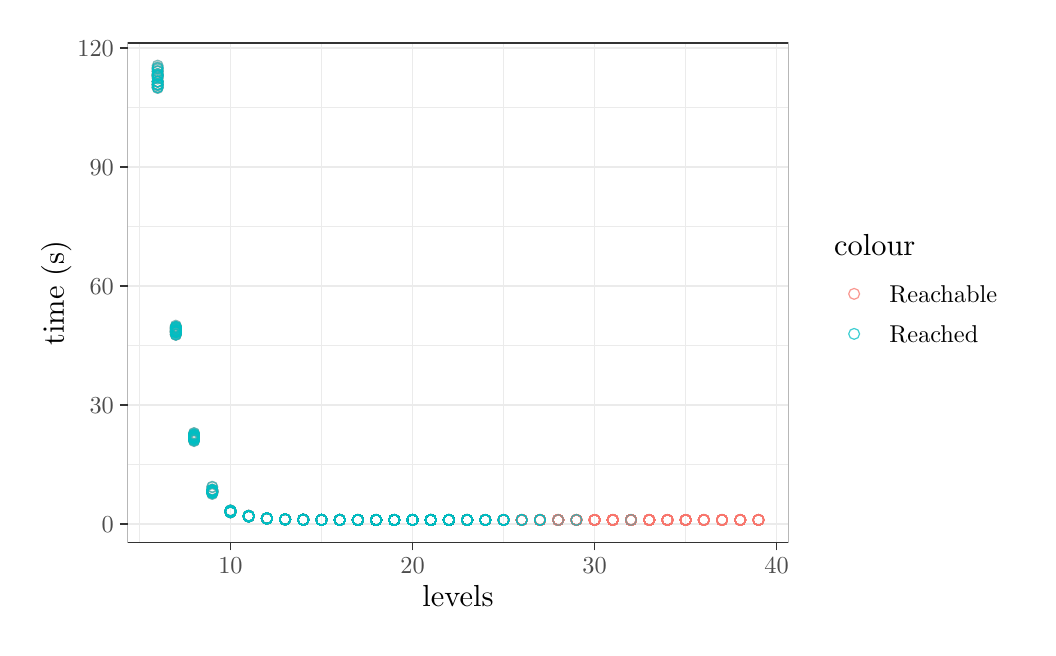
\begin{tikzpicture}[x=1pt,y=1pt]
\definecolor{fillColor}{RGB}{255,255,255}
\path[use as bounding box,fill=fillColor,fill opacity=0.00] (0,0) rectangle (361.35,216.81);
\begin{scope}
\path[clip] (  0.00,  0.00) rectangle (361.35,216.81);
\definecolor{drawColor}{RGB}{255,255,255}
\definecolor{fillColor}{RGB}{255,255,255}

\path[draw=drawColor,line width= 0.6pt,line join=round,line cap=round,fill=fillColor] (  0.00,  0.00) rectangle (361.35,216.81);
\end{scope}
\begin{scope}
\path[clip] ( 36.11, 30.69) rectangle (274.92,211.31);
\definecolor{fillColor}{RGB}{255,255,255}

\path[fill=fillColor] ( 36.11, 30.69) rectangle (274.92,211.31);
\definecolor{drawColor}{gray}{0.92}

\path[draw=drawColor,line width= 0.3pt,line join=round] ( 36.11, 59.01) --
	(274.92, 59.01);

\path[draw=drawColor,line width= 0.3pt,line join=round] ( 36.11,102.00) --
	(274.92,102.00);

\path[draw=drawColor,line width= 0.3pt,line join=round] ( 36.11,145.00) --
	(274.92,145.00);

\path[draw=drawColor,line width= 0.3pt,line join=round] ( 36.11,187.99) --
	(274.92,187.99);

\path[draw=drawColor,line width= 0.3pt,line join=round] ( 40.39, 30.69) --
	( 40.39,211.31);

\path[draw=drawColor,line width= 0.3pt,line join=round] (106.17, 30.69) --
	(106.17,211.31);

\path[draw=drawColor,line width= 0.3pt,line join=round] (171.96, 30.69) --
	(171.96,211.31);

\path[draw=drawColor,line width= 0.3pt,line join=round] (237.75, 30.69) --
	(237.75,211.31);

\path[draw=drawColor,line width= 0.6pt,line join=round] ( 36.11, 37.51) --
	(274.92, 37.51);

\path[draw=drawColor,line width= 0.6pt,line join=round] ( 36.11, 80.50) --
	(274.92, 80.50);

\path[draw=drawColor,line width= 0.6pt,line join=round] ( 36.11,123.50) --
	(274.92,123.50);

\path[draw=drawColor,line width= 0.6pt,line join=round] ( 36.11,166.50) --
	(274.92,166.50);

\path[draw=drawColor,line width= 0.6pt,line join=round] ( 36.11,209.49) --
	(274.92,209.49);

\path[draw=drawColor,line width= 0.6pt,line join=round] ( 73.28, 30.69) --
	( 73.28,211.31);

\path[draw=drawColor,line width= 0.6pt,line join=round] (139.07, 30.69) --
	(139.07,211.31);

\path[draw=drawColor,line width= 0.6pt,line join=round] (204.85, 30.69) --
	(204.85,211.31);

\path[draw=drawColor,line width= 0.6pt,line join=round] (270.64, 30.69) --
	(270.64,211.31);
\definecolor{drawColor}{RGB}{248,118,109}

\path[draw=drawColor,draw opacity=0.50,line width= 0.4pt,line join=round,line cap=round] ( 73.28, 41.76) circle (  1.96);

\path[draw=drawColor,draw opacity=0.50,line width= 0.4pt,line join=round,line cap=round] ( 73.28, 42.14) circle (  1.96);

\path[draw=drawColor,draw opacity=0.50,line width= 0.4pt,line join=round,line cap=round] ( 73.28, 42.16) circle (  1.96);

\path[draw=drawColor,draw opacity=0.50,line width= 0.4pt,line join=round,line cap=round] ( 73.28, 41.89) circle (  1.96);

\path[draw=drawColor,draw opacity=0.50,line width= 0.4pt,line join=round,line cap=round] ( 73.28, 42.10) circle (  1.96);

\path[draw=drawColor,draw opacity=0.50,line width= 0.4pt,line join=round,line cap=round] ( 73.28, 41.89) circle (  1.96);

\path[draw=drawColor,draw opacity=0.50,line width= 0.4pt,line join=round,line cap=round] ( 73.28, 41.75) circle (  1.96);

\path[draw=drawColor,draw opacity=0.50,line width= 0.4pt,line join=round,line cap=round] ( 73.28, 41.85) circle (  1.96);

\path[draw=drawColor,draw opacity=0.50,line width= 0.4pt,line join=round,line cap=round] ( 73.28, 42.06) circle (  1.96);

\path[draw=drawColor,draw opacity=0.50,line width= 0.4pt,line join=round,line cap=round] ( 73.28, 42.19) circle (  1.96);

\path[draw=drawColor,draw opacity=0.50,line width= 0.4pt,line join=round,line cap=round] ( 73.28, 41.97) circle (  1.96);

\path[draw=drawColor,draw opacity=0.50,line width= 0.4pt,line join=round,line cap=round] ( 73.28, 42.19) circle (  1.96);

\path[draw=drawColor,draw opacity=0.50,line width= 0.4pt,line join=round,line cap=round] ( 73.28, 42.02) circle (  1.96);

\path[draw=drawColor,draw opacity=0.50,line width= 0.4pt,line join=round,line cap=round] ( 73.28, 41.93) circle (  1.96);

\path[draw=drawColor,draw opacity=0.50,line width= 0.4pt,line join=round,line cap=round] ( 73.28, 42.22) circle (  1.96);

\path[draw=drawColor,draw opacity=0.50,line width= 0.4pt,line join=round,line cap=round] ( 73.28, 42.00) circle (  1.96);

\path[draw=drawColor,draw opacity=0.50,line width= 0.4pt,line join=round,line cap=round] ( 73.28, 41.96) circle (  1.96);

\path[draw=drawColor,draw opacity=0.50,line width= 0.4pt,line join=round,line cap=round] ( 73.28, 42.08) circle (  1.96);

\path[draw=drawColor,draw opacity=0.50,line width= 0.4pt,line join=round,line cap=round] ( 73.28, 42.30) circle (  1.96);

\path[draw=drawColor,draw opacity=0.50,line width= 0.4pt,line join=round,line cap=round] ( 73.28, 41.83) circle (  1.96);

\path[draw=drawColor,draw opacity=0.50,line width= 0.4pt,line join=round,line cap=round] ( 73.28, 41.87) circle (  1.96);

\path[draw=drawColor,draw opacity=0.50,line width= 0.4pt,line join=round,line cap=round] ( 73.28, 41.89) circle (  1.96);

\path[draw=drawColor,draw opacity=0.50,line width= 0.4pt,line join=round,line cap=round] ( 73.28, 41.95) circle (  1.96);

\path[draw=drawColor,draw opacity=0.50,line width= 0.4pt,line join=round,line cap=round] ( 73.28, 41.92) circle (  1.96);

\path[draw=drawColor,draw opacity=0.50,line width= 0.4pt,line join=round,line cap=round] ( 73.28, 41.90) circle (  1.96);

\path[draw=drawColor,draw opacity=0.50,line width= 0.4pt,line join=round,line cap=round] ( 73.28, 42.10) circle (  1.96);

\path[draw=drawColor,draw opacity=0.50,line width= 0.4pt,line join=round,line cap=round] ( 73.28, 41.96) circle (  1.96);

\path[draw=drawColor,draw opacity=0.50,line width= 0.4pt,line join=round,line cap=round] ( 73.28, 42.08) circle (  1.96);

\path[draw=drawColor,draw opacity=0.50,line width= 0.4pt,line join=round,line cap=round] ( 73.28, 42.22) circle (  1.96);

\path[draw=drawColor,draw opacity=0.50,line width= 0.4pt,line join=round,line cap=round] ( 73.28, 41.90) circle (  1.96);

\path[draw=drawColor,draw opacity=0.50,line width= 0.4pt,line join=round,line cap=round] ( 73.28, 42.28) circle (  1.96);

\path[draw=drawColor,draw opacity=0.50,line width= 0.4pt,line join=round,line cap=round] ( 73.28, 42.11) circle (  1.96);

\path[draw=drawColor,draw opacity=0.50,line width= 0.4pt,line join=round,line cap=round] ( 73.28, 42.03) circle (  1.96);

\path[draw=drawColor,draw opacity=0.50,line width= 0.4pt,line join=round,line cap=round] ( 73.28, 42.18) circle (  1.96);

\path[draw=drawColor,draw opacity=0.50,line width= 0.4pt,line join=round,line cap=round] ( 79.86, 40.17) circle (  1.96);

\path[draw=drawColor,draw opacity=0.50,line width= 0.4pt,line join=round,line cap=round] ( 79.86, 40.28) circle (  1.96);

\path[draw=drawColor,draw opacity=0.50,line width= 0.4pt,line join=round,line cap=round] ( 79.86, 40.22) circle (  1.96);

\path[draw=drawColor,draw opacity=0.50,line width= 0.4pt,line join=round,line cap=round] ( 79.86, 40.33) circle (  1.96);

\path[draw=drawColor,draw opacity=0.50,line width= 0.4pt,line join=round,line cap=round] ( 79.86, 40.47) circle (  1.96);

\path[draw=drawColor,draw opacity=0.50,line width= 0.4pt,line join=round,line cap=round] ( 79.86, 40.19) circle (  1.96);

\path[draw=drawColor,draw opacity=0.50,line width= 0.4pt,line join=round,line cap=round] ( 79.86, 40.29) circle (  1.96);

\path[draw=drawColor,draw opacity=0.50,line width= 0.4pt,line join=round,line cap=round] ( 79.86, 40.33) circle (  1.96);

\path[draw=drawColor,draw opacity=0.50,line width= 0.4pt,line join=round,line cap=round] ( 79.86, 40.20) circle (  1.96);

\path[draw=drawColor,draw opacity=0.50,line width= 0.4pt,line join=round,line cap=round] ( 79.86, 40.39) circle (  1.96);

\path[draw=drawColor,draw opacity=0.50,line width= 0.4pt,line join=round,line cap=round] ( 79.86, 40.27) circle (  1.96);

\path[draw=drawColor,draw opacity=0.50,line width= 0.4pt,line join=round,line cap=round] ( 79.86, 40.38) circle (  1.96);

\path[draw=drawColor,draw opacity=0.50,line width= 0.4pt,line join=round,line cap=round] ( 79.86, 40.37) circle (  1.96);

\path[draw=drawColor,draw opacity=0.50,line width= 0.4pt,line join=round,line cap=round] ( 79.86, 40.27) circle (  1.96);

\path[draw=drawColor,draw opacity=0.50,line width= 0.4pt,line join=round,line cap=round] ( 79.86, 40.28) circle (  1.96);

\path[draw=drawColor,draw opacity=0.50,line width= 0.4pt,line join=round,line cap=round] ( 79.86, 40.42) circle (  1.96);

\path[draw=drawColor,draw opacity=0.50,line width= 0.4pt,line join=round,line cap=round] ( 79.86, 40.23) circle (  1.96);

\path[draw=drawColor,draw opacity=0.50,line width= 0.4pt,line join=round,line cap=round] ( 79.86, 40.37) circle (  1.96);

\path[draw=drawColor,draw opacity=0.50,line width= 0.4pt,line join=round,line cap=round] ( 79.86, 40.29) circle (  1.96);

\path[draw=drawColor,draw opacity=0.50,line width= 0.4pt,line join=round,line cap=round] ( 79.86, 40.34) circle (  1.96);

\path[draw=drawColor,draw opacity=0.50,line width= 0.4pt,line join=round,line cap=round] ( 79.86, 40.29) circle (  1.96);

\path[draw=drawColor,draw opacity=0.50,line width= 0.4pt,line join=round,line cap=round] ( 79.86, 40.30) circle (  1.96);

\path[draw=drawColor,draw opacity=0.50,line width= 0.4pt,line join=round,line cap=round] ( 79.86, 40.18) circle (  1.96);

\path[draw=drawColor,draw opacity=0.50,line width= 0.4pt,line join=round,line cap=round] ( 79.86, 40.37) circle (  1.96);

\path[draw=drawColor,draw opacity=0.50,line width= 0.4pt,line join=round,line cap=round] ( 79.86, 40.21) circle (  1.96);

\path[draw=drawColor,draw opacity=0.50,line width= 0.4pt,line join=round,line cap=round] ( 79.86, 40.36) circle (  1.96);

\path[draw=drawColor,draw opacity=0.50,line width= 0.4pt,line join=round,line cap=round] ( 79.86, 40.30) circle (  1.96);

\path[draw=drawColor,draw opacity=0.50,line width= 0.4pt,line join=round,line cap=round] ( 79.86, 40.35) circle (  1.96);

\path[draw=drawColor,draw opacity=0.50,line width= 0.4pt,line join=round,line cap=round] ( 79.86, 40.33) circle (  1.96);

\path[draw=drawColor,draw opacity=0.50,line width= 0.4pt,line join=round,line cap=round] ( 79.86, 40.22) circle (  1.96);

\path[draw=drawColor,draw opacity=0.50,line width= 0.4pt,line join=round,line cap=round] ( 79.86, 40.37) circle (  1.96);

\path[draw=drawColor,draw opacity=0.50,line width= 0.4pt,line join=round,line cap=round] ( 79.86, 40.29) circle (  1.96);

\path[draw=drawColor,draw opacity=0.50,line width= 0.4pt,line join=round,line cap=round] ( 79.86, 40.34) circle (  1.96);

\path[draw=drawColor,draw opacity=0.50,line width= 0.4pt,line join=round,line cap=round] ( 86.44, 39.46) circle (  1.96);

\path[draw=drawColor,draw opacity=0.50,line width= 0.4pt,line join=round,line cap=round] ( 86.44, 39.51) circle (  1.96);

\path[draw=drawColor,draw opacity=0.50,line width= 0.4pt,line join=round,line cap=round] ( 86.44, 39.49) circle (  1.96);

\path[draw=drawColor,draw opacity=0.50,line width= 0.4pt,line join=round,line cap=round] ( 86.44, 39.53) circle (  1.96);

\path[draw=drawColor,draw opacity=0.50,line width= 0.4pt,line join=round,line cap=round] ( 86.44, 39.43) circle (  1.96);

\path[draw=drawColor,draw opacity=0.50,line width= 0.4pt,line join=round,line cap=round] ( 86.44, 39.46) circle (  1.96);

\path[draw=drawColor,draw opacity=0.50,line width= 0.4pt,line join=round,line cap=round] ( 86.44, 39.45) circle (  1.96);

\path[draw=drawColor,draw opacity=0.50,line width= 0.4pt,line join=round,line cap=round] ( 86.44, 39.39) circle (  1.96);

\path[draw=drawColor,draw opacity=0.50,line width= 0.4pt,line join=round,line cap=round] ( 86.44, 39.47) circle (  1.96);

\path[draw=drawColor,draw opacity=0.50,line width= 0.4pt,line join=round,line cap=round] ( 86.44, 39.49) circle (  1.96);

\path[draw=drawColor,draw opacity=0.50,line width= 0.4pt,line join=round,line cap=round] ( 86.44, 39.53) circle (  1.96);

\path[draw=drawColor,draw opacity=0.50,line width= 0.4pt,line join=round,line cap=round] ( 86.44, 39.49) circle (  1.96);

\path[draw=drawColor,draw opacity=0.50,line width= 0.4pt,line join=round,line cap=round] ( 86.44, 39.48) circle (  1.96);

\path[draw=drawColor,draw opacity=0.50,line width= 0.4pt,line join=round,line cap=round] ( 86.44, 39.47) circle (  1.96);

\path[draw=drawColor,draw opacity=0.50,line width= 0.4pt,line join=round,line cap=round] ( 86.44, 39.42) circle (  1.96);

\path[draw=drawColor,draw opacity=0.50,line width= 0.4pt,line join=round,line cap=round] ( 86.44, 39.54) circle (  1.96);

\path[draw=drawColor,draw opacity=0.50,line width= 0.4pt,line join=round,line cap=round] ( 86.44, 39.49) circle (  1.96);

\path[draw=drawColor,draw opacity=0.50,line width= 0.4pt,line join=round,line cap=round] ( 86.44, 39.47) circle (  1.96);

\path[draw=drawColor,draw opacity=0.50,line width= 0.4pt,line join=round,line cap=round] ( 86.44, 39.49) circle (  1.96);

\path[draw=drawColor,draw opacity=0.50,line width= 0.4pt,line join=round,line cap=round] ( 86.44, 39.40) circle (  1.96);

\path[draw=drawColor,draw opacity=0.50,line width= 0.4pt,line join=round,line cap=round] ( 86.44, 39.38) circle (  1.96);

\path[draw=drawColor,draw opacity=0.50,line width= 0.4pt,line join=round,line cap=round] ( 86.44, 39.49) circle (  1.96);

\path[draw=drawColor,draw opacity=0.50,line width= 0.4pt,line join=round,line cap=round] ( 86.44, 39.40) circle (  1.96);

\path[draw=drawColor,draw opacity=0.50,line width= 0.4pt,line join=round,line cap=round] ( 86.44, 39.56) circle (  1.96);

\path[draw=drawColor,draw opacity=0.50,line width= 0.4pt,line join=round,line cap=round] ( 86.44, 39.51) circle (  1.96);

\path[draw=drawColor,draw opacity=0.50,line width= 0.4pt,line join=round,line cap=round] ( 86.44, 39.49) circle (  1.96);

\path[draw=drawColor,draw opacity=0.50,line width= 0.4pt,line join=round,line cap=round] ( 86.44, 39.53) circle (  1.96);

\path[draw=drawColor,draw opacity=0.50,line width= 0.4pt,line join=round,line cap=round] ( 86.44, 39.44) circle (  1.96);

\path[draw=drawColor,draw opacity=0.50,line width= 0.4pt,line join=round,line cap=round] ( 86.44, 39.50) circle (  1.96);

\path[draw=drawColor,draw opacity=0.50,line width= 0.4pt,line join=round,line cap=round] ( 86.44, 39.40) circle (  1.96);

\path[draw=drawColor,draw opacity=0.50,line width= 0.4pt,line join=round,line cap=round] ( 86.44, 39.46) circle (  1.96);

\path[draw=drawColor,draw opacity=0.50,line width= 0.4pt,line join=round,line cap=round] ( 86.44, 39.49) circle (  1.96);

\path[draw=drawColor,draw opacity=0.50,line width= 0.4pt,line join=round,line cap=round] ( 86.44, 39.47) circle (  1.96);

\path[draw=drawColor,draw opacity=0.50,line width= 0.4pt,line join=round,line cap=round] ( 93.02, 39.14) circle (  1.96);

\path[draw=drawColor,draw opacity=0.50,line width= 0.4pt,line join=round,line cap=round] ( 93.02, 39.12) circle (  1.96);

\path[draw=drawColor,draw opacity=0.50,line width= 0.4pt,line join=round,line cap=round] ( 93.02, 39.12) circle (  1.96);

\path[draw=drawColor,draw opacity=0.50,line width= 0.4pt,line join=round,line cap=round] ( 93.02, 39.15) circle (  1.96);

\path[draw=drawColor,draw opacity=0.50,line width= 0.4pt,line join=round,line cap=round] ( 93.02, 39.08) circle (  1.96);

\path[draw=drawColor,draw opacity=0.50,line width= 0.4pt,line join=round,line cap=round] ( 93.02, 39.15) circle (  1.96);

\path[draw=drawColor,draw opacity=0.50,line width= 0.4pt,line join=round,line cap=round] ( 93.02, 39.14) circle (  1.96);

\path[draw=drawColor,draw opacity=0.50,line width= 0.4pt,line join=round,line cap=round] ( 93.02, 39.12) circle (  1.96);

\path[draw=drawColor,draw opacity=0.50,line width= 0.4pt,line join=round,line cap=round] ( 93.02, 39.15) circle (  1.96);

\path[draw=drawColor,draw opacity=0.50,line width= 0.4pt,line join=round,line cap=round] ( 93.02, 39.09) circle (  1.96);

\path[draw=drawColor,draw opacity=0.50,line width= 0.4pt,line join=round,line cap=round] ( 93.02, 39.13) circle (  1.96);

\path[draw=drawColor,draw opacity=0.50,line width= 0.4pt,line join=round,line cap=round] ( 93.02, 39.16) circle (  1.96);

\path[draw=drawColor,draw opacity=0.50,line width= 0.4pt,line join=round,line cap=round] ( 93.02, 39.11) circle (  1.96);

\path[draw=drawColor,draw opacity=0.50,line width= 0.4pt,line join=round,line cap=round] ( 93.02, 39.19) circle (  1.96);

\path[draw=drawColor,draw opacity=0.50,line width= 0.4pt,line join=round,line cap=round] ( 93.02, 39.12) circle (  1.96);

\path[draw=drawColor,draw opacity=0.50,line width= 0.4pt,line join=round,line cap=round] ( 93.02, 39.14) circle (  1.96);

\path[draw=drawColor,draw opacity=0.50,line width= 0.4pt,line join=round,line cap=round] ( 93.02, 39.09) circle (  1.96);

\path[draw=drawColor,draw opacity=0.50,line width= 0.4pt,line join=round,line cap=round] ( 93.02, 39.12) circle (  1.96);

\path[draw=drawColor,draw opacity=0.50,line width= 0.4pt,line join=round,line cap=round] ( 93.02, 39.08) circle (  1.96);

\path[draw=drawColor,draw opacity=0.50,line width= 0.4pt,line join=round,line cap=round] ( 93.02, 39.17) circle (  1.96);

\path[draw=drawColor,draw opacity=0.50,line width= 0.4pt,line join=round,line cap=round] ( 93.02, 39.13) circle (  1.96);

\path[draw=drawColor,draw opacity=0.50,line width= 0.4pt,line join=round,line cap=round] ( 93.02, 39.12) circle (  1.96);

\path[draw=drawColor,draw opacity=0.50,line width= 0.4pt,line join=round,line cap=round] ( 93.02, 39.09) circle (  1.96);

\path[draw=drawColor,draw opacity=0.50,line width= 0.4pt,line join=round,line cap=round] ( 93.02, 39.09) circle (  1.96);

\path[draw=drawColor,draw opacity=0.50,line width= 0.4pt,line join=round,line cap=round] ( 93.02, 39.18) circle (  1.96);

\path[draw=drawColor,draw opacity=0.50,line width= 0.4pt,line join=round,line cap=round] ( 93.02, 39.12) circle (  1.96);

\path[draw=drawColor,draw opacity=0.50,line width= 0.4pt,line join=round,line cap=round] ( 93.02, 39.09) circle (  1.96);

\path[draw=drawColor,draw opacity=0.50,line width= 0.4pt,line join=round,line cap=round] ( 93.02, 39.15) circle (  1.96);

\path[draw=drawColor,draw opacity=0.50,line width= 0.4pt,line join=round,line cap=round] ( 93.02, 39.10) circle (  1.96);

\path[draw=drawColor,draw opacity=0.50,line width= 0.4pt,line join=round,line cap=round] ( 93.02, 39.13) circle (  1.96);

\path[draw=drawColor,draw opacity=0.50,line width= 0.4pt,line join=round,line cap=round] ( 93.02, 39.12) circle (  1.96);

\path[draw=drawColor,draw opacity=0.50,line width= 0.4pt,line join=round,line cap=round] ( 93.02, 39.12) circle (  1.96);

\path[draw=drawColor,draw opacity=0.50,line width= 0.4pt,line join=round,line cap=round] ( 93.02, 39.16) circle (  1.96);

\path[draw=drawColor,draw opacity=0.50,line width= 0.4pt,line join=round,line cap=round] ( 99.60, 39.00) circle (  1.96);

\path[draw=drawColor,draw opacity=0.50,line width= 0.4pt,line join=round,line cap=round] ( 99.60, 39.00) circle (  1.96);

\path[draw=drawColor,draw opacity=0.50,line width= 0.4pt,line join=round,line cap=round] ( 99.60, 39.00) circle (  1.96);

\path[draw=drawColor,draw opacity=0.50,line width= 0.4pt,line join=round,line cap=round] ( 99.60, 39.01) circle (  1.96);

\path[draw=drawColor,draw opacity=0.50,line width= 0.4pt,line join=round,line cap=round] ( 99.60, 38.98) circle (  1.96);

\path[draw=drawColor,draw opacity=0.50,line width= 0.4pt,line join=round,line cap=round] ( 99.60, 39.00) circle (  1.96);

\path[draw=drawColor,draw opacity=0.50,line width= 0.4pt,line join=round,line cap=round] ( 99.60, 39.00) circle (  1.96);

\path[draw=drawColor,draw opacity=0.50,line width= 0.4pt,line join=round,line cap=round] ( 99.60, 39.03) circle (  1.96);

\path[draw=drawColor,draw opacity=0.50,line width= 0.4pt,line join=round,line cap=round] ( 99.60, 39.00) circle (  1.96);

\path[draw=drawColor,draw opacity=0.50,line width= 0.4pt,line join=round,line cap=round] ( 99.60, 38.97) circle (  1.96);

\path[draw=drawColor,draw opacity=0.50,line width= 0.4pt,line join=round,line cap=round] ( 99.60, 39.03) circle (  1.96);

\path[draw=drawColor,draw opacity=0.50,line width= 0.4pt,line join=round,line cap=round] ( 99.60, 39.01) circle (  1.96);

\path[draw=drawColor,draw opacity=0.50,line width= 0.4pt,line join=round,line cap=round] ( 99.60, 38.99) circle (  1.96);

\path[draw=drawColor,draw opacity=0.50,line width= 0.4pt,line join=round,line cap=round] ( 99.60, 39.00) circle (  1.96);

\path[draw=drawColor,draw opacity=0.50,line width= 0.4pt,line join=round,line cap=round] ( 99.60, 38.98) circle (  1.96);

\path[draw=drawColor,draw opacity=0.50,line width= 0.4pt,line join=round,line cap=round] ( 99.60, 38.99) circle (  1.96);

\path[draw=drawColor,draw opacity=0.50,line width= 0.4pt,line join=round,line cap=round] ( 99.60, 39.04) circle (  1.96);

\path[draw=drawColor,draw opacity=0.50,line width= 0.4pt,line join=round,line cap=round] ( 99.60, 39.01) circle (  1.96);

\path[draw=drawColor,draw opacity=0.50,line width= 0.4pt,line join=round,line cap=round] ( 99.60, 38.97) circle (  1.96);

\path[draw=drawColor,draw opacity=0.50,line width= 0.4pt,line join=round,line cap=round] ( 99.60, 39.00) circle (  1.96);

\path[draw=drawColor,draw opacity=0.50,line width= 0.4pt,line join=round,line cap=round] ( 99.60, 38.97) circle (  1.96);

\path[draw=drawColor,draw opacity=0.50,line width= 0.4pt,line join=round,line cap=round] ( 99.60, 39.01) circle (  1.96);

\path[draw=drawColor,draw opacity=0.50,line width= 0.4pt,line join=round,line cap=round] ( 99.60, 39.01) circle (  1.96);

\path[draw=drawColor,draw opacity=0.50,line width= 0.4pt,line join=round,line cap=round] ( 99.60, 39.00) circle (  1.96);

\path[draw=drawColor,draw opacity=0.50,line width= 0.4pt,line join=round,line cap=round] ( 99.60, 38.98) circle (  1.96);

\path[draw=drawColor,draw opacity=0.50,line width= 0.4pt,line join=round,line cap=round] ( 99.60, 38.97) circle (  1.96);

\path[draw=drawColor,draw opacity=0.50,line width= 0.4pt,line join=round,line cap=round] ( 99.60, 39.02) circle (  1.96);

\path[draw=drawColor,draw opacity=0.50,line width= 0.4pt,line join=round,line cap=round] ( 99.60, 39.01) circle (  1.96);

\path[draw=drawColor,draw opacity=0.50,line width= 0.4pt,line join=round,line cap=round] ( 99.60, 38.98) circle (  1.96);

\path[draw=drawColor,draw opacity=0.50,line width= 0.4pt,line join=round,line cap=round] ( 99.60, 39.00) circle (  1.96);

\path[draw=drawColor,draw opacity=0.50,line width= 0.4pt,line join=round,line cap=round] ( 99.60, 38.97) circle (  1.96);

\path[draw=drawColor,draw opacity=0.50,line width= 0.4pt,line join=round,line cap=round] ( 99.60, 39.00) circle (  1.96);

\path[draw=drawColor,draw opacity=0.50,line width= 0.4pt,line join=round,line cap=round] ( 99.60, 39.00) circle (  1.96);

\path[draw=drawColor,draw opacity=0.50,line width= 0.4pt,line join=round,line cap=round] (106.17, 38.93) circle (  1.96);

\path[draw=drawColor,draw opacity=0.50,line width= 0.4pt,line join=round,line cap=round] (106.17, 38.93) circle (  1.96);

\path[draw=drawColor,draw opacity=0.50,line width= 0.4pt,line join=round,line cap=round] (106.17, 38.94) circle (  1.96);

\path[draw=drawColor,draw opacity=0.50,line width= 0.4pt,line join=round,line cap=round] (106.17, 38.94) circle (  1.96);

\path[draw=drawColor,draw opacity=0.50,line width= 0.4pt,line join=round,line cap=round] (106.17, 38.95) circle (  1.96);

\path[draw=drawColor,draw opacity=0.50,line width= 0.4pt,line join=round,line cap=round] (106.17, 38.94) circle (  1.96);

\path[draw=drawColor,draw opacity=0.50,line width= 0.4pt,line join=round,line cap=round] (106.17, 38.95) circle (  1.96);

\path[draw=drawColor,draw opacity=0.50,line width= 0.4pt,line join=round,line cap=round] (106.17, 38.96) circle (  1.96);

\path[draw=drawColor,draw opacity=0.50,line width= 0.4pt,line join=round,line cap=round] (106.17, 38.94) circle (  1.96);

\path[draw=drawColor,draw opacity=0.50,line width= 0.4pt,line join=round,line cap=round] (106.17, 38.95) circle (  1.96);

\path[draw=drawColor,draw opacity=0.50,line width= 0.4pt,line join=round,line cap=round] (106.17, 38.95) circle (  1.96);

\path[draw=drawColor,draw opacity=0.50,line width= 0.4pt,line join=round,line cap=round] (106.17, 38.94) circle (  1.96);

\path[draw=drawColor,draw opacity=0.50,line width= 0.4pt,line join=round,line cap=round] (106.17, 38.95) circle (  1.96);

\path[draw=drawColor,draw opacity=0.50,line width= 0.4pt,line join=round,line cap=round] (106.17, 38.97) circle (  1.96);

\path[draw=drawColor,draw opacity=0.50,line width= 0.4pt,line join=round,line cap=round] (106.17, 38.96) circle (  1.96);

\path[draw=drawColor,draw opacity=0.50,line width= 0.4pt,line join=round,line cap=round] (106.17, 38.95) circle (  1.96);

\path[draw=drawColor,draw opacity=0.50,line width= 0.4pt,line join=round,line cap=round] (106.17, 38.93) circle (  1.96);

\path[draw=drawColor,draw opacity=0.50,line width= 0.4pt,line join=round,line cap=round] (106.17, 38.96) circle (  1.96);

\path[draw=drawColor,draw opacity=0.50,line width= 0.4pt,line join=round,line cap=round] (106.17, 38.96) circle (  1.96);

\path[draw=drawColor,draw opacity=0.50,line width= 0.4pt,line join=round,line cap=round] (106.17, 38.95) circle (  1.96);

\path[draw=drawColor,draw opacity=0.50,line width= 0.4pt,line join=round,line cap=round] (106.17, 38.96) circle (  1.96);

\path[draw=drawColor,draw opacity=0.50,line width= 0.4pt,line join=round,line cap=round] (106.17, 38.95) circle (  1.96);

\path[draw=drawColor,draw opacity=0.50,line width= 0.4pt,line join=round,line cap=round] (106.17, 38.96) circle (  1.96);

\path[draw=drawColor,draw opacity=0.50,line width= 0.4pt,line join=round,line cap=round] (106.17, 38.94) circle (  1.96);

\path[draw=drawColor,draw opacity=0.50,line width= 0.4pt,line join=round,line cap=round] (106.17, 38.95) circle (  1.96);

\path[draw=drawColor,draw opacity=0.50,line width= 0.4pt,line join=round,line cap=round] (106.17, 38.95) circle (  1.96);

\path[draw=drawColor,draw opacity=0.50,line width= 0.4pt,line join=round,line cap=round] (106.17, 38.94) circle (  1.96);

\path[draw=drawColor,draw opacity=0.50,line width= 0.4pt,line join=round,line cap=round] (106.17, 38.96) circle (  1.96);

\path[draw=drawColor,draw opacity=0.50,line width= 0.4pt,line join=round,line cap=round] (106.17, 38.95) circle (  1.96);

\path[draw=drawColor,draw opacity=0.50,line width= 0.4pt,line join=round,line cap=round] (106.17, 38.94) circle (  1.96);

\path[draw=drawColor,draw opacity=0.50,line width= 0.4pt,line join=round,line cap=round] (106.17, 38.96) circle (  1.96);

\path[draw=drawColor,draw opacity=0.50,line width= 0.4pt,line join=round,line cap=round] (106.17, 38.96) circle (  1.96);

\path[draw=drawColor,draw opacity=0.50,line width= 0.4pt,line join=round,line cap=round] (106.17, 38.94) circle (  1.96);

\path[draw=drawColor,draw opacity=0.50,line width= 0.4pt,line join=round,line cap=round] (112.75, 38.93) circle (  1.96);

\path[draw=drawColor,draw opacity=0.50,line width= 0.4pt,line join=round,line cap=round] (112.75, 38.94) circle (  1.96);

\path[draw=drawColor,draw opacity=0.50,line width= 0.4pt,line join=round,line cap=round] (112.75, 38.94) circle (  1.96);

\path[draw=drawColor,draw opacity=0.50,line width= 0.4pt,line join=round,line cap=round] (112.75, 38.94) circle (  1.96);

\path[draw=drawColor,draw opacity=0.50,line width= 0.4pt,line join=round,line cap=round] (112.75, 38.92) circle (  1.96);

\path[draw=drawColor,draw opacity=0.50,line width= 0.4pt,line join=round,line cap=round] (112.75, 38.94) circle (  1.96);

\path[draw=drawColor,draw opacity=0.50,line width= 0.4pt,line join=round,line cap=round] (112.75, 38.95) circle (  1.96);

\path[draw=drawColor,draw opacity=0.50,line width= 0.4pt,line join=round,line cap=round] (112.75, 38.93) circle (  1.96);

\path[draw=drawColor,draw opacity=0.50,line width= 0.4pt,line join=round,line cap=round] (112.75, 38.93) circle (  1.96);

\path[draw=drawColor,draw opacity=0.50,line width= 0.4pt,line join=round,line cap=round] (112.75, 38.93) circle (  1.96);

\path[draw=drawColor,draw opacity=0.50,line width= 0.4pt,line join=round,line cap=round] (112.75, 38.94) circle (  1.96);

\path[draw=drawColor,draw opacity=0.50,line width= 0.4pt,line join=round,line cap=round] (112.75, 38.95) circle (  1.96);

\path[draw=drawColor,draw opacity=0.50,line width= 0.4pt,line join=round,line cap=round] (112.75, 38.94) circle (  1.96);

\path[draw=drawColor,draw opacity=0.50,line width= 0.4pt,line join=round,line cap=round] (112.75, 38.93) circle (  1.96);

\path[draw=drawColor,draw opacity=0.50,line width= 0.4pt,line join=round,line cap=round] (112.75, 38.94) circle (  1.96);

\path[draw=drawColor,draw opacity=0.50,line width= 0.4pt,line join=round,line cap=round] (112.75, 38.94) circle (  1.96);

\path[draw=drawColor,draw opacity=0.50,line width= 0.4pt,line join=round,line cap=round] (112.75, 38.94) circle (  1.96);

\path[draw=drawColor,draw opacity=0.50,line width= 0.4pt,line join=round,line cap=round] (112.75, 38.94) circle (  1.96);

\path[draw=drawColor,draw opacity=0.50,line width= 0.4pt,line join=round,line cap=round] (112.75, 38.94) circle (  1.96);

\path[draw=drawColor,draw opacity=0.50,line width= 0.4pt,line join=round,line cap=round] (112.75, 38.93) circle (  1.96);

\path[draw=drawColor,draw opacity=0.50,line width= 0.4pt,line join=round,line cap=round] (112.75, 38.94) circle (  1.96);

\path[draw=drawColor,draw opacity=0.50,line width= 0.4pt,line join=round,line cap=round] (112.75, 38.93) circle (  1.96);

\path[draw=drawColor,draw opacity=0.50,line width= 0.4pt,line join=round,line cap=round] (112.75, 38.93) circle (  1.96);

\path[draw=drawColor,draw opacity=0.50,line width= 0.4pt,line join=round,line cap=round] (112.75, 38.93) circle (  1.96);

\path[draw=drawColor,draw opacity=0.50,line width= 0.4pt,line join=round,line cap=round] (112.75, 38.95) circle (  1.96);

\path[draw=drawColor,draw opacity=0.50,line width= 0.4pt,line join=round,line cap=round] (112.75, 38.95) circle (  1.96);

\path[draw=drawColor,draw opacity=0.50,line width= 0.4pt,line join=round,line cap=round] (112.75, 38.92) circle (  1.96);

\path[draw=drawColor,draw opacity=0.50,line width= 0.4pt,line join=round,line cap=round] (112.75, 38.94) circle (  1.96);

\path[draw=drawColor,draw opacity=0.50,line width= 0.4pt,line join=round,line cap=round] (112.75, 38.92) circle (  1.96);

\path[draw=drawColor,draw opacity=0.50,line width= 0.4pt,line join=round,line cap=round] (112.75, 38.95) circle (  1.96);

\path[draw=drawColor,draw opacity=0.50,line width= 0.4pt,line join=round,line cap=round] (112.75, 38.95) circle (  1.96);

\path[draw=drawColor,draw opacity=0.50,line width= 0.4pt,line join=round,line cap=round] (112.75, 38.93) circle (  1.96);

\path[draw=drawColor,draw opacity=0.50,line width= 0.4pt,line join=round,line cap=round] (112.75, 38.93) circle (  1.96);

\path[draw=drawColor,draw opacity=0.50,line width= 0.4pt,line join=round,line cap=round] (119.33, 38.92) circle (  1.96);

\path[draw=drawColor,draw opacity=0.50,line width= 0.4pt,line join=round,line cap=round] (119.33, 38.94) circle (  1.96);

\path[draw=drawColor,draw opacity=0.50,line width= 0.4pt,line join=round,line cap=round] (119.33, 38.92) circle (  1.96);

\path[draw=drawColor,draw opacity=0.50,line width= 0.4pt,line join=round,line cap=round] (119.33, 38.93) circle (  1.96);

\path[draw=drawColor,draw opacity=0.50,line width= 0.4pt,line join=round,line cap=round] (119.33, 38.92) circle (  1.96);

\path[draw=drawColor,draw opacity=0.50,line width= 0.4pt,line join=round,line cap=round] (119.33, 38.93) circle (  1.96);

\path[draw=drawColor,draw opacity=0.50,line width= 0.4pt,line join=round,line cap=round] (119.33, 38.92) circle (  1.96);

\path[draw=drawColor,draw opacity=0.50,line width= 0.4pt,line join=round,line cap=round] (119.33, 38.93) circle (  1.96);

\path[draw=drawColor,draw opacity=0.50,line width= 0.4pt,line join=round,line cap=round] (119.33, 38.94) circle (  1.96);

\path[draw=drawColor,draw opacity=0.50,line width= 0.4pt,line join=round,line cap=round] (119.33, 38.93) circle (  1.96);

\path[draw=drawColor,draw opacity=0.50,line width= 0.4pt,line join=round,line cap=round] (119.33, 38.94) circle (  1.96);

\path[draw=drawColor,draw opacity=0.50,line width= 0.4pt,line join=round,line cap=round] (119.33, 38.93) circle (  1.96);

\path[draw=drawColor,draw opacity=0.50,line width= 0.4pt,line join=round,line cap=round] (119.33, 38.92) circle (  1.96);

\path[draw=drawColor,draw opacity=0.50,line width= 0.4pt,line join=round,line cap=round] (119.33, 38.93) circle (  1.96);

\path[draw=drawColor,draw opacity=0.50,line width= 0.4pt,line join=round,line cap=round] (119.33, 38.93) circle (  1.96);

\path[draw=drawColor,draw opacity=0.50,line width= 0.4pt,line join=round,line cap=round] (119.33, 38.93) circle (  1.96);

\path[draw=drawColor,draw opacity=0.50,line width= 0.4pt,line join=round,line cap=round] (119.33, 38.93) circle (  1.96);

\path[draw=drawColor,draw opacity=0.50,line width= 0.4pt,line join=round,line cap=round] (119.33, 38.94) circle (  1.96);

\path[draw=drawColor,draw opacity=0.50,line width= 0.4pt,line join=round,line cap=round] (119.33, 38.92) circle (  1.96);

\path[draw=drawColor,draw opacity=0.50,line width= 0.4pt,line join=round,line cap=round] (119.33, 38.92) circle (  1.96);

\path[draw=drawColor,draw opacity=0.50,line width= 0.4pt,line join=round,line cap=round] (119.33, 38.93) circle (  1.96);

\path[draw=drawColor,draw opacity=0.50,line width= 0.4pt,line join=round,line cap=round] (119.33, 38.93) circle (  1.96);

\path[draw=drawColor,draw opacity=0.50,line width= 0.4pt,line join=round,line cap=round] (119.33, 38.91) circle (  1.96);

\path[draw=drawColor,draw opacity=0.50,line width= 0.4pt,line join=round,line cap=round] (119.33, 38.93) circle (  1.96);

\path[draw=drawColor,draw opacity=0.50,line width= 0.4pt,line join=round,line cap=round] (119.33, 38.93) circle (  1.96);

\path[draw=drawColor,draw opacity=0.50,line width= 0.4pt,line join=round,line cap=round] (119.33, 38.92) circle (  1.96);

\path[draw=drawColor,draw opacity=0.50,line width= 0.4pt,line join=round,line cap=round] (119.33, 38.94) circle (  1.96);

\path[draw=drawColor,draw opacity=0.50,line width= 0.4pt,line join=round,line cap=round] (119.33, 38.93) circle (  1.96);

\path[draw=drawColor,draw opacity=0.50,line width= 0.4pt,line join=round,line cap=round] (119.33, 38.93) circle (  1.96);

\path[draw=drawColor,draw opacity=0.50,line width= 0.4pt,line join=round,line cap=round] (119.33, 38.93) circle (  1.96);

\path[draw=drawColor,draw opacity=0.50,line width= 0.4pt,line join=round,line cap=round] (119.33, 38.93) circle (  1.96);

\path[draw=drawColor,draw opacity=0.50,line width= 0.4pt,line join=round,line cap=round] (119.33, 38.92) circle (  1.96);

\path[draw=drawColor,draw opacity=0.50,line width= 0.4pt,line join=round,line cap=round] (119.33, 38.92) circle (  1.96);

\path[draw=drawColor,draw opacity=0.50,line width= 0.4pt,line join=round,line cap=round] (125.91, 38.94) circle (  1.96);

\path[draw=drawColor,draw opacity=0.50,line width= 0.4pt,line join=round,line cap=round] (125.91, 38.92) circle (  1.96);

\path[draw=drawColor,draw opacity=0.50,line width= 0.4pt,line join=round,line cap=round] (125.91, 38.92) circle (  1.96);

\path[draw=drawColor,draw opacity=0.50,line width= 0.4pt,line join=round,line cap=round] (125.91, 38.92) circle (  1.96);

\path[draw=drawColor,draw opacity=0.50,line width= 0.4pt,line join=round,line cap=round] (125.91, 38.92) circle (  1.96);

\path[draw=drawColor,draw opacity=0.50,line width= 0.4pt,line join=round,line cap=round] (125.91, 38.92) circle (  1.96);

\path[draw=drawColor,draw opacity=0.50,line width= 0.4pt,line join=round,line cap=round] (125.91, 38.93) circle (  1.96);

\path[draw=drawColor,draw opacity=0.50,line width= 0.4pt,line join=round,line cap=round] (125.91, 38.92) circle (  1.96);

\path[draw=drawColor,draw opacity=0.50,line width= 0.4pt,line join=round,line cap=round] (125.91, 38.92) circle (  1.96);

\path[draw=drawColor,draw opacity=0.50,line width= 0.4pt,line join=round,line cap=round] (125.91, 38.92) circle (  1.96);

\path[draw=drawColor,draw opacity=0.50,line width= 0.4pt,line join=round,line cap=round] (125.91, 38.92) circle (  1.96);

\path[draw=drawColor,draw opacity=0.50,line width= 0.4pt,line join=round,line cap=round] (125.91, 38.93) circle (  1.96);

\path[draw=drawColor,draw opacity=0.50,line width= 0.4pt,line join=round,line cap=round] (125.91, 38.93) circle (  1.96);

\path[draw=drawColor,draw opacity=0.50,line width= 0.4pt,line join=round,line cap=round] (125.91, 38.92) circle (  1.96);

\path[draw=drawColor,draw opacity=0.50,line width= 0.4pt,line join=round,line cap=round] (125.91, 38.91) circle (  1.96);

\path[draw=drawColor,draw opacity=0.50,line width= 0.4pt,line join=round,line cap=round] (125.91, 38.92) circle (  1.96);

\path[draw=drawColor,draw opacity=0.50,line width= 0.4pt,line join=round,line cap=round] (125.91, 38.92) circle (  1.96);

\path[draw=drawColor,draw opacity=0.50,line width= 0.4pt,line join=round,line cap=round] (125.91, 38.93) circle (  1.96);

\path[draw=drawColor,draw opacity=0.50,line width= 0.4pt,line join=round,line cap=round] (125.91, 38.92) circle (  1.96);

\path[draw=drawColor,draw opacity=0.50,line width= 0.4pt,line join=round,line cap=round] (125.91, 38.93) circle (  1.96);

\path[draw=drawColor,draw opacity=0.50,line width= 0.4pt,line join=round,line cap=round] (125.91, 38.92) circle (  1.96);

\path[draw=drawColor,draw opacity=0.50,line width= 0.4pt,line join=round,line cap=round] (125.91, 38.92) circle (  1.96);

\path[draw=drawColor,draw opacity=0.50,line width= 0.4pt,line join=round,line cap=round] (125.91, 38.93) circle (  1.96);

\path[draw=drawColor,draw opacity=0.50,line width= 0.4pt,line join=round,line cap=round] (125.91, 38.92) circle (  1.96);

\path[draw=drawColor,draw opacity=0.50,line width= 0.4pt,line join=round,line cap=round] (125.91, 38.93) circle (  1.96);

\path[draw=drawColor,draw opacity=0.50,line width= 0.4pt,line join=round,line cap=round] (125.91, 38.92) circle (  1.96);

\path[draw=drawColor,draw opacity=0.50,line width= 0.4pt,line join=round,line cap=round] (125.91, 38.92) circle (  1.96);

\path[draw=drawColor,draw opacity=0.50,line width= 0.4pt,line join=round,line cap=round] (125.91, 38.94) circle (  1.96);

\path[draw=drawColor,draw opacity=0.50,line width= 0.4pt,line join=round,line cap=round] (125.91, 38.92) circle (  1.96);

\path[draw=drawColor,draw opacity=0.50,line width= 0.4pt,line join=round,line cap=round] (125.91, 38.92) circle (  1.96);

\path[draw=drawColor,draw opacity=0.50,line width= 0.4pt,line join=round,line cap=round] (125.91, 38.92) circle (  1.96);

\path[draw=drawColor,draw opacity=0.50,line width= 0.4pt,line join=round,line cap=round] (125.91, 38.92) circle (  1.96);

\path[draw=drawColor,draw opacity=0.50,line width= 0.4pt,line join=round,line cap=round] (125.91, 38.92) circle (  1.96);

\path[draw=drawColor,draw opacity=0.50,line width= 0.4pt,line join=round,line cap=round] (132.49, 38.93) circle (  1.96);

\path[draw=drawColor,draw opacity=0.50,line width= 0.4pt,line join=round,line cap=round] (132.49, 38.93) circle (  1.96);

\path[draw=drawColor,draw opacity=0.50,line width= 0.4pt,line join=round,line cap=round] (132.49, 38.91) circle (  1.96);

\path[draw=drawColor,draw opacity=0.50,line width= 0.4pt,line join=round,line cap=round] (132.49, 38.93) circle (  1.96);

\path[draw=drawColor,draw opacity=0.50,line width= 0.4pt,line join=round,line cap=round] (132.49, 38.92) circle (  1.96);

\path[draw=drawColor,draw opacity=0.50,line width= 0.4pt,line join=round,line cap=round] (132.49, 38.92) circle (  1.96);

\path[draw=drawColor,draw opacity=0.50,line width= 0.4pt,line join=round,line cap=round] (132.49, 38.92) circle (  1.96);

\path[draw=drawColor,draw opacity=0.50,line width= 0.4pt,line join=round,line cap=round] (132.49, 38.91) circle (  1.96);

\path[draw=drawColor,draw opacity=0.50,line width= 0.4pt,line join=round,line cap=round] (132.49, 38.92) circle (  1.96);

\path[draw=drawColor,draw opacity=0.50,line width= 0.4pt,line join=round,line cap=round] (132.49, 38.92) circle (  1.96);

\path[draw=drawColor,draw opacity=0.50,line width= 0.4pt,line join=round,line cap=round] (132.49, 38.93) circle (  1.96);

\path[draw=drawColor,draw opacity=0.50,line width= 0.4pt,line join=round,line cap=round] (132.49, 38.93) circle (  1.96);

\path[draw=drawColor,draw opacity=0.50,line width= 0.4pt,line join=round,line cap=round] (132.49, 38.92) circle (  1.96);

\path[draw=drawColor,draw opacity=0.50,line width= 0.4pt,line join=round,line cap=round] (132.49, 38.93) circle (  1.96);

\path[draw=drawColor,draw opacity=0.50,line width= 0.4pt,line join=round,line cap=round] (132.49, 38.93) circle (  1.96);

\path[draw=drawColor,draw opacity=0.50,line width= 0.4pt,line join=round,line cap=round] (132.49, 38.92) circle (  1.96);

\path[draw=drawColor,draw opacity=0.50,line width= 0.4pt,line join=round,line cap=round] (132.49, 38.93) circle (  1.96);

\path[draw=drawColor,draw opacity=0.50,line width= 0.4pt,line join=round,line cap=round] (132.49, 38.93) circle (  1.96);

\path[draw=drawColor,draw opacity=0.50,line width= 0.4pt,line join=round,line cap=round] (132.49, 38.93) circle (  1.96);

\path[draw=drawColor,draw opacity=0.50,line width= 0.4pt,line join=round,line cap=round] (132.49, 38.93) circle (  1.96);

\path[draw=drawColor,draw opacity=0.50,line width= 0.4pt,line join=round,line cap=round] (132.49, 38.93) circle (  1.96);

\path[draw=drawColor,draw opacity=0.50,line width= 0.4pt,line join=round,line cap=round] (132.49, 38.93) circle (  1.96);

\path[draw=drawColor,draw opacity=0.50,line width= 0.4pt,line join=round,line cap=round] (132.49, 38.93) circle (  1.96);

\path[draw=drawColor,draw opacity=0.50,line width= 0.4pt,line join=round,line cap=round] (132.49, 38.92) circle (  1.96);

\path[draw=drawColor,draw opacity=0.50,line width= 0.4pt,line join=round,line cap=round] (132.49, 38.93) circle (  1.96);

\path[draw=drawColor,draw opacity=0.50,line width= 0.4pt,line join=round,line cap=round] (132.49, 38.93) circle (  1.96);

\path[draw=drawColor,draw opacity=0.50,line width= 0.4pt,line join=round,line cap=round] (132.49, 38.92) circle (  1.96);

\path[draw=drawColor,draw opacity=0.50,line width= 0.4pt,line join=round,line cap=round] (132.49, 38.92) circle (  1.96);

\path[draw=drawColor,draw opacity=0.50,line width= 0.4pt,line join=round,line cap=round] (132.49, 38.92) circle (  1.96);

\path[draw=drawColor,draw opacity=0.50,line width= 0.4pt,line join=round,line cap=round] (132.49, 38.93) circle (  1.96);

\path[draw=drawColor,draw opacity=0.50,line width= 0.4pt,line join=round,line cap=round] (132.49, 38.93) circle (  1.96);

\path[draw=drawColor,draw opacity=0.50,line width= 0.4pt,line join=round,line cap=round] (132.49, 38.92) circle (  1.96);

\path[draw=drawColor,draw opacity=0.50,line width= 0.4pt,line join=round,line cap=round] (132.49, 38.91) circle (  1.96);

\path[draw=drawColor,draw opacity=0.50,line width= 0.4pt,line join=round,line cap=round] (139.07, 38.92) circle (  1.96);

\path[draw=drawColor,draw opacity=0.50,line width= 0.4pt,line join=round,line cap=round] (139.07, 38.92) circle (  1.96);

\path[draw=drawColor,draw opacity=0.50,line width= 0.4pt,line join=round,line cap=round] (139.07, 38.93) circle (  1.96);

\path[draw=drawColor,draw opacity=0.50,line width= 0.4pt,line join=round,line cap=round] (139.07, 38.92) circle (  1.96);

\path[draw=drawColor,draw opacity=0.50,line width= 0.4pt,line join=round,line cap=round] (139.07, 38.93) circle (  1.96);

\path[draw=drawColor,draw opacity=0.50,line width= 0.4pt,line join=round,line cap=round] (139.07, 38.93) circle (  1.96);

\path[draw=drawColor,draw opacity=0.50,line width= 0.4pt,line join=round,line cap=round] (139.07, 38.92) circle (  1.96);

\path[draw=drawColor,draw opacity=0.50,line width= 0.4pt,line join=round,line cap=round] (139.07, 38.93) circle (  1.96);

\path[draw=drawColor,draw opacity=0.50,line width= 0.4pt,line join=round,line cap=round] (139.07, 38.93) circle (  1.96);

\path[draw=drawColor,draw opacity=0.50,line width= 0.4pt,line join=round,line cap=round] (139.07, 38.92) circle (  1.96);

\path[draw=drawColor,draw opacity=0.50,line width= 0.4pt,line join=round,line cap=round] (139.07, 38.92) circle (  1.96);

\path[draw=drawColor,draw opacity=0.50,line width= 0.4pt,line join=round,line cap=round] (139.07, 38.92) circle (  1.96);

\path[draw=drawColor,draw opacity=0.50,line width= 0.4pt,line join=round,line cap=round] (139.07, 38.93) circle (  1.96);

\path[draw=drawColor,draw opacity=0.50,line width= 0.4pt,line join=round,line cap=round] (139.07, 38.92) circle (  1.96);

\path[draw=drawColor,draw opacity=0.50,line width= 0.4pt,line join=round,line cap=round] (139.07, 38.93) circle (  1.96);

\path[draw=drawColor,draw opacity=0.50,line width= 0.4pt,line join=round,line cap=round] (139.07, 38.92) circle (  1.96);

\path[draw=drawColor,draw opacity=0.50,line width= 0.4pt,line join=round,line cap=round] (139.07, 38.93) circle (  1.96);

\path[draw=drawColor,draw opacity=0.50,line width= 0.4pt,line join=round,line cap=round] (139.07, 38.93) circle (  1.96);

\path[draw=drawColor,draw opacity=0.50,line width= 0.4pt,line join=round,line cap=round] (139.07, 38.91) circle (  1.96);

\path[draw=drawColor,draw opacity=0.50,line width= 0.4pt,line join=round,line cap=round] (139.07, 38.92) circle (  1.96);

\path[draw=drawColor,draw opacity=0.50,line width= 0.4pt,line join=round,line cap=round] (139.07, 38.92) circle (  1.96);

\path[draw=drawColor,draw opacity=0.50,line width= 0.4pt,line join=round,line cap=round] (139.07, 38.93) circle (  1.96);

\path[draw=drawColor,draw opacity=0.50,line width= 0.4pt,line join=round,line cap=round] (139.07, 38.93) circle (  1.96);

\path[draw=drawColor,draw opacity=0.50,line width= 0.4pt,line join=round,line cap=round] (139.07, 38.93) circle (  1.96);

\path[draw=drawColor,draw opacity=0.50,line width= 0.4pt,line join=round,line cap=round] (139.07, 38.94) circle (  1.96);

\path[draw=drawColor,draw opacity=0.50,line width= 0.4pt,line join=round,line cap=round] (139.07, 38.95) circle (  1.96);

\path[draw=drawColor,draw opacity=0.50,line width= 0.4pt,line join=round,line cap=round] (139.07, 38.94) circle (  1.96);

\path[draw=drawColor,draw opacity=0.50,line width= 0.4pt,line join=round,line cap=round] (139.07, 38.93) circle (  1.96);

\path[draw=drawColor,draw opacity=0.50,line width= 0.4pt,line join=round,line cap=round] (139.07, 38.93) circle (  1.96);

\path[draw=drawColor,draw opacity=0.50,line width= 0.4pt,line join=round,line cap=round] (139.07, 38.92) circle (  1.96);

\path[draw=drawColor,draw opacity=0.50,line width= 0.4pt,line join=round,line cap=round] (139.07, 38.93) circle (  1.96);

\path[draw=drawColor,draw opacity=0.50,line width= 0.4pt,line join=round,line cap=round] (139.07, 38.92) circle (  1.96);

\path[draw=drawColor,draw opacity=0.50,line width= 0.4pt,line join=round,line cap=round] (139.07, 38.92) circle (  1.96);

\path[draw=drawColor,draw opacity=0.50,line width= 0.4pt,line join=round,line cap=round] (145.65, 38.92) circle (  1.96);

\path[draw=drawColor,draw opacity=0.50,line width= 0.4pt,line join=round,line cap=round] (145.65, 38.93) circle (  1.96);

\path[draw=drawColor,draw opacity=0.50,line width= 0.4pt,line join=round,line cap=round] (145.65, 38.94) circle (  1.96);

\path[draw=drawColor,draw opacity=0.50,line width= 0.4pt,line join=round,line cap=round] (145.65, 38.92) circle (  1.96);

\path[draw=drawColor,draw opacity=0.50,line width= 0.4pt,line join=round,line cap=round] (145.65, 38.92) circle (  1.96);

\path[draw=drawColor,draw opacity=0.50,line width= 0.4pt,line join=round,line cap=round] (145.65, 38.93) circle (  1.96);

\path[draw=drawColor,draw opacity=0.50,line width= 0.4pt,line join=round,line cap=round] (145.65, 38.92) circle (  1.96);

\path[draw=drawColor,draw opacity=0.50,line width= 0.4pt,line join=round,line cap=round] (145.65, 38.92) circle (  1.96);

\path[draw=drawColor,draw opacity=0.50,line width= 0.4pt,line join=round,line cap=round] (145.65, 38.92) circle (  1.96);

\path[draw=drawColor,draw opacity=0.50,line width= 0.4pt,line join=round,line cap=round] (145.65, 38.94) circle (  1.96);

\path[draw=drawColor,draw opacity=0.50,line width= 0.4pt,line join=round,line cap=round] (145.65, 38.92) circle (  1.96);

\path[draw=drawColor,draw opacity=0.50,line width= 0.4pt,line join=round,line cap=round] (145.65, 38.94) circle (  1.96);

\path[draw=drawColor,draw opacity=0.50,line width= 0.4pt,line join=round,line cap=round] (145.65, 38.92) circle (  1.96);

\path[draw=drawColor,draw opacity=0.50,line width= 0.4pt,line join=round,line cap=round] (145.65, 38.93) circle (  1.96);

\path[draw=drawColor,draw opacity=0.50,line width= 0.4pt,line join=round,line cap=round] (145.65, 38.92) circle (  1.96);

\path[draw=drawColor,draw opacity=0.50,line width= 0.4pt,line join=round,line cap=round] (145.65, 38.93) circle (  1.96);

\path[draw=drawColor,draw opacity=0.50,line width= 0.4pt,line join=round,line cap=round] (145.65, 38.92) circle (  1.96);

\path[draw=drawColor,draw opacity=0.50,line width= 0.4pt,line join=round,line cap=round] (145.65, 38.92) circle (  1.96);

\path[draw=drawColor,draw opacity=0.50,line width= 0.4pt,line join=round,line cap=round] (145.65, 38.94) circle (  1.96);

\path[draw=drawColor,draw opacity=0.50,line width= 0.4pt,line join=round,line cap=round] (145.65, 38.93) circle (  1.96);

\path[draw=drawColor,draw opacity=0.50,line width= 0.4pt,line join=round,line cap=round] (145.65, 38.92) circle (  1.96);

\path[draw=drawColor,draw opacity=0.50,line width= 0.4pt,line join=round,line cap=round] (145.65, 38.93) circle (  1.96);

\path[draw=drawColor,draw opacity=0.50,line width= 0.4pt,line join=round,line cap=round] (145.65, 38.92) circle (  1.96);

\path[draw=drawColor,draw opacity=0.50,line width= 0.4pt,line join=round,line cap=round] (145.65, 38.93) circle (  1.96);

\path[draw=drawColor,draw opacity=0.50,line width= 0.4pt,line join=round,line cap=round] (145.65, 38.92) circle (  1.96);

\path[draw=drawColor,draw opacity=0.50,line width= 0.4pt,line join=round,line cap=round] (145.65, 38.93) circle (  1.96);

\path[draw=drawColor,draw opacity=0.50,line width= 0.4pt,line join=round,line cap=round] (145.65, 38.92) circle (  1.96);

\path[draw=drawColor,draw opacity=0.50,line width= 0.4pt,line join=round,line cap=round] (145.65, 38.94) circle (  1.96);

\path[draw=drawColor,draw opacity=0.50,line width= 0.4pt,line join=round,line cap=round] (145.65, 38.93) circle (  1.96);

\path[draw=drawColor,draw opacity=0.50,line width= 0.4pt,line join=round,line cap=round] (145.65, 38.93) circle (  1.96);

\path[draw=drawColor,draw opacity=0.50,line width= 0.4pt,line join=round,line cap=round] (145.65, 38.93) circle (  1.96);

\path[draw=drawColor,draw opacity=0.50,line width= 0.4pt,line join=round,line cap=round] (145.65, 38.93) circle (  1.96);

\path[draw=drawColor,draw opacity=0.50,line width= 0.4pt,line join=round,line cap=round] (145.65, 38.93) circle (  1.96);

\path[draw=drawColor,draw opacity=0.50,line width= 0.4pt,line join=round,line cap=round] (152.22, 38.93) circle (  1.96);

\path[draw=drawColor,draw opacity=0.50,line width= 0.4pt,line join=round,line cap=round] (152.22, 38.93) circle (  1.96);

\path[draw=drawColor,draw opacity=0.50,line width= 0.4pt,line join=round,line cap=round] (152.22, 38.93) circle (  1.96);

\path[draw=drawColor,draw opacity=0.50,line width= 0.4pt,line join=round,line cap=round] (152.22, 38.92) circle (  1.96);

\path[draw=drawColor,draw opacity=0.50,line width= 0.4pt,line join=round,line cap=round] (152.22, 38.92) circle (  1.96);

\path[draw=drawColor,draw opacity=0.50,line width= 0.4pt,line join=round,line cap=round] (152.22, 38.93) circle (  1.96);

\path[draw=drawColor,draw opacity=0.50,line width= 0.4pt,line join=round,line cap=round] (152.22, 38.94) circle (  1.96);

\path[draw=drawColor,draw opacity=0.50,line width= 0.4pt,line join=round,line cap=round] (152.22, 38.93) circle (  1.96);

\path[draw=drawColor,draw opacity=0.50,line width= 0.4pt,line join=round,line cap=round] (152.22, 38.91) circle (  1.96);

\path[draw=drawColor,draw opacity=0.50,line width= 0.4pt,line join=round,line cap=round] (152.22, 38.92) circle (  1.96);

\path[draw=drawColor,draw opacity=0.50,line width= 0.4pt,line join=round,line cap=round] (152.22, 38.94) circle (  1.96);

\path[draw=drawColor,draw opacity=0.50,line width= 0.4pt,line join=round,line cap=round] (152.22, 38.94) circle (  1.96);

\path[draw=drawColor,draw opacity=0.50,line width= 0.4pt,line join=round,line cap=round] (152.22, 38.92) circle (  1.96);

\path[draw=drawColor,draw opacity=0.50,line width= 0.4pt,line join=round,line cap=round] (152.22, 38.92) circle (  1.96);

\path[draw=drawColor,draw opacity=0.50,line width= 0.4pt,line join=round,line cap=round] (152.22, 38.92) circle (  1.96);

\path[draw=drawColor,draw opacity=0.50,line width= 0.4pt,line join=round,line cap=round] (152.22, 38.94) circle (  1.96);

\path[draw=drawColor,draw opacity=0.50,line width= 0.4pt,line join=round,line cap=round] (152.22, 38.93) circle (  1.96);

\path[draw=drawColor,draw opacity=0.50,line width= 0.4pt,line join=round,line cap=round] (152.22, 38.93) circle (  1.96);

\path[draw=drawColor,draw opacity=0.50,line width= 0.4pt,line join=round,line cap=round] (152.22, 38.93) circle (  1.96);

\path[draw=drawColor,draw opacity=0.50,line width= 0.4pt,line join=round,line cap=round] (152.22, 38.92) circle (  1.96);

\path[draw=drawColor,draw opacity=0.50,line width= 0.4pt,line join=round,line cap=round] (152.22, 38.92) circle (  1.96);

\path[draw=drawColor,draw opacity=0.50,line width= 0.4pt,line join=round,line cap=round] (152.22, 38.92) circle (  1.96);

\path[draw=drawColor,draw opacity=0.50,line width= 0.4pt,line join=round,line cap=round] (152.22, 38.93) circle (  1.96);

\path[draw=drawColor,draw opacity=0.50,line width= 0.4pt,line join=round,line cap=round] (152.22, 38.94) circle (  1.96);

\path[draw=drawColor,draw opacity=0.50,line width= 0.4pt,line join=round,line cap=round] (152.22, 38.93) circle (  1.96);

\path[draw=drawColor,draw opacity=0.50,line width= 0.4pt,line join=round,line cap=round] (152.22, 38.92) circle (  1.96);

\path[draw=drawColor,draw opacity=0.50,line width= 0.4pt,line join=round,line cap=round] (152.22, 38.93) circle (  1.96);

\path[draw=drawColor,draw opacity=0.50,line width= 0.4pt,line join=round,line cap=round] (152.22, 38.93) circle (  1.96);

\path[draw=drawColor,draw opacity=0.50,line width= 0.4pt,line join=round,line cap=round] (152.22, 38.92) circle (  1.96);

\path[draw=drawColor,draw opacity=0.50,line width= 0.4pt,line join=round,line cap=round] (152.22, 38.92) circle (  1.96);

\path[draw=drawColor,draw opacity=0.50,line width= 0.4pt,line join=round,line cap=round] (152.22, 38.93) circle (  1.96);

\path[draw=drawColor,draw opacity=0.50,line width= 0.4pt,line join=round,line cap=round] (152.22, 38.93) circle (  1.96);

\path[draw=drawColor,draw opacity=0.50,line width= 0.4pt,line join=round,line cap=round] (152.22, 38.92) circle (  1.96);

\path[draw=drawColor,draw opacity=0.50,line width= 0.4pt,line join=round,line cap=round] (158.80, 38.93) circle (  1.96);

\path[draw=drawColor,draw opacity=0.50,line width= 0.4pt,line join=round,line cap=round] (158.80, 38.93) circle (  1.96);

\path[draw=drawColor,draw opacity=0.50,line width= 0.4pt,line join=round,line cap=round] (158.80, 38.93) circle (  1.96);

\path[draw=drawColor,draw opacity=0.50,line width= 0.4pt,line join=round,line cap=round] (158.80, 38.93) circle (  1.96);

\path[draw=drawColor,draw opacity=0.50,line width= 0.4pt,line join=round,line cap=round] (158.80, 38.92) circle (  1.96);

\path[draw=drawColor,draw opacity=0.50,line width= 0.4pt,line join=round,line cap=round] (158.80, 38.93) circle (  1.96);

\path[draw=drawColor,draw opacity=0.50,line width= 0.4pt,line join=round,line cap=round] (158.80, 38.92) circle (  1.96);

\path[draw=drawColor,draw opacity=0.50,line width= 0.4pt,line join=round,line cap=round] (158.80, 38.92) circle (  1.96);

\path[draw=drawColor,draw opacity=0.50,line width= 0.4pt,line join=round,line cap=round] (158.80, 38.93) circle (  1.96);

\path[draw=drawColor,draw opacity=0.50,line width= 0.4pt,line join=round,line cap=round] (158.80, 38.92) circle (  1.96);

\path[draw=drawColor,draw opacity=0.50,line width= 0.4pt,line join=round,line cap=round] (158.80, 38.93) circle (  1.96);

\path[draw=drawColor,draw opacity=0.50,line width= 0.4pt,line join=round,line cap=round] (158.80, 38.94) circle (  1.96);

\path[draw=drawColor,draw opacity=0.50,line width= 0.4pt,line join=round,line cap=round] (158.80, 38.92) circle (  1.96);

\path[draw=drawColor,draw opacity=0.50,line width= 0.4pt,line join=round,line cap=round] (158.80, 38.93) circle (  1.96);

\path[draw=drawColor,draw opacity=0.50,line width= 0.4pt,line join=round,line cap=round] (158.80, 38.92) circle (  1.96);

\path[draw=drawColor,draw opacity=0.50,line width= 0.4pt,line join=round,line cap=round] (158.80, 38.92) circle (  1.96);

\path[draw=drawColor,draw opacity=0.50,line width= 0.4pt,line join=round,line cap=round] (158.80, 38.92) circle (  1.96);

\path[draw=drawColor,draw opacity=0.50,line width= 0.4pt,line join=round,line cap=round] (158.80, 38.93) circle (  1.96);

\path[draw=drawColor,draw opacity=0.50,line width= 0.4pt,line join=round,line cap=round] (158.80, 38.93) circle (  1.96);

\path[draw=drawColor,draw opacity=0.50,line width= 0.4pt,line join=round,line cap=round] (158.80, 38.94) circle (  1.96);

\path[draw=drawColor,draw opacity=0.50,line width= 0.4pt,line join=round,line cap=round] (158.80, 38.92) circle (  1.96);

\path[draw=drawColor,draw opacity=0.50,line width= 0.4pt,line join=round,line cap=round] (158.80, 38.92) circle (  1.96);

\path[draw=drawColor,draw opacity=0.50,line width= 0.4pt,line join=round,line cap=round] (158.80, 38.93) circle (  1.96);

\path[draw=drawColor,draw opacity=0.50,line width= 0.4pt,line join=round,line cap=round] (158.80, 38.92) circle (  1.96);

\path[draw=drawColor,draw opacity=0.50,line width= 0.4pt,line join=round,line cap=round] (158.80, 38.92) circle (  1.96);

\path[draw=drawColor,draw opacity=0.50,line width= 0.4pt,line join=round,line cap=round] (158.80, 38.92) circle (  1.96);

\path[draw=drawColor,draw opacity=0.50,line width= 0.4pt,line join=round,line cap=round] (158.80, 38.93) circle (  1.96);

\path[draw=drawColor,draw opacity=0.50,line width= 0.4pt,line join=round,line cap=round] (158.80, 38.92) circle (  1.96);

\path[draw=drawColor,draw opacity=0.50,line width= 0.4pt,line join=round,line cap=round] (158.80, 38.92) circle (  1.96);

\path[draw=drawColor,draw opacity=0.50,line width= 0.4pt,line join=round,line cap=round] (158.80, 38.92) circle (  1.96);

\path[draw=drawColor,draw opacity=0.50,line width= 0.4pt,line join=round,line cap=round] (158.80, 38.94) circle (  1.96);

\path[draw=drawColor,draw opacity=0.50,line width= 0.4pt,line join=round,line cap=round] (158.80, 38.92) circle (  1.96);

\path[draw=drawColor,draw opacity=0.50,line width= 0.4pt,line join=round,line cap=round] (158.80, 38.92) circle (  1.96);

\path[draw=drawColor,draw opacity=0.50,line width= 0.4pt,line join=round,line cap=round] (165.38, 38.92) circle (  1.96);

\path[draw=drawColor,draw opacity=0.50,line width= 0.4pt,line join=round,line cap=round] (165.38, 38.93) circle (  1.96);

\path[draw=drawColor,draw opacity=0.50,line width= 0.4pt,line join=round,line cap=round] (165.38, 38.94) circle (  1.96);

\path[draw=drawColor,draw opacity=0.50,line width= 0.4pt,line join=round,line cap=round] (165.38, 38.93) circle (  1.96);

\path[draw=drawColor,draw opacity=0.50,line width= 0.4pt,line join=round,line cap=round] (165.38, 38.93) circle (  1.96);

\path[draw=drawColor,draw opacity=0.50,line width= 0.4pt,line join=round,line cap=round] (165.38, 38.92) circle (  1.96);

\path[draw=drawColor,draw opacity=0.50,line width= 0.4pt,line join=round,line cap=round] (165.38, 38.92) circle (  1.96);

\path[draw=drawColor,draw opacity=0.50,line width= 0.4pt,line join=round,line cap=round] (165.38, 38.93) circle (  1.96);

\path[draw=drawColor,draw opacity=0.50,line width= 0.4pt,line join=round,line cap=round] (165.38, 38.91) circle (  1.96);

\path[draw=drawColor,draw opacity=0.50,line width= 0.4pt,line join=round,line cap=round] (165.38, 38.94) circle (  1.96);

\path[draw=drawColor,draw opacity=0.50,line width= 0.4pt,line join=round,line cap=round] (165.38, 38.93) circle (  1.96);

\path[draw=drawColor,draw opacity=0.50,line width= 0.4pt,line join=round,line cap=round] (165.38, 38.92) circle (  1.96);

\path[draw=drawColor,draw opacity=0.50,line width= 0.4pt,line join=round,line cap=round] (165.38, 38.92) circle (  1.96);

\path[draw=drawColor,draw opacity=0.50,line width= 0.4pt,line join=round,line cap=round] (165.38, 38.92) circle (  1.96);

\path[draw=drawColor,draw opacity=0.50,line width= 0.4pt,line join=round,line cap=round] (165.38, 38.93) circle (  1.96);

\path[draw=drawColor,draw opacity=0.50,line width= 0.4pt,line join=round,line cap=round] (165.38, 38.93) circle (  1.96);

\path[draw=drawColor,draw opacity=0.50,line width= 0.4pt,line join=round,line cap=round] (165.38, 38.93) circle (  1.96);

\path[draw=drawColor,draw opacity=0.50,line width= 0.4pt,line join=round,line cap=round] (165.38, 38.93) circle (  1.96);

\path[draw=drawColor,draw opacity=0.50,line width= 0.4pt,line join=round,line cap=round] (165.38, 38.93) circle (  1.96);

\path[draw=drawColor,draw opacity=0.50,line width= 0.4pt,line join=round,line cap=round] (165.38, 38.93) circle (  1.96);

\path[draw=drawColor,draw opacity=0.50,line width= 0.4pt,line join=round,line cap=round] (165.38, 38.93) circle (  1.96);

\path[draw=drawColor,draw opacity=0.50,line width= 0.4pt,line join=round,line cap=round] (165.38, 38.92) circle (  1.96);

\path[draw=drawColor,draw opacity=0.50,line width= 0.4pt,line join=round,line cap=round] (165.38, 38.92) circle (  1.96);

\path[draw=drawColor,draw opacity=0.50,line width= 0.4pt,line join=round,line cap=round] (165.38, 38.94) circle (  1.96);

\path[draw=drawColor,draw opacity=0.50,line width= 0.4pt,line join=round,line cap=round] (165.38, 38.93) circle (  1.96);

\path[draw=drawColor,draw opacity=0.50,line width= 0.4pt,line join=round,line cap=round] (165.38, 38.92) circle (  1.96);

\path[draw=drawColor,draw opacity=0.50,line width= 0.4pt,line join=round,line cap=round] (165.38, 38.93) circle (  1.96);

\path[draw=drawColor,draw opacity=0.50,line width= 0.4pt,line join=round,line cap=round] (165.38, 38.93) circle (  1.96);

\path[draw=drawColor,draw opacity=0.50,line width= 0.4pt,line join=round,line cap=round] (165.38, 38.92) circle (  1.96);

\path[draw=drawColor,draw opacity=0.50,line width= 0.4pt,line join=round,line cap=round] (165.38, 38.92) circle (  1.96);

\path[draw=drawColor,draw opacity=0.50,line width= 0.4pt,line join=round,line cap=round] (165.38, 38.92) circle (  1.96);

\path[draw=drawColor,draw opacity=0.50,line width= 0.4pt,line join=round,line cap=round] (165.38, 38.92) circle (  1.96);

\path[draw=drawColor,draw opacity=0.50,line width= 0.4pt,line join=round,line cap=round] (165.38, 38.92) circle (  1.96);

\path[draw=drawColor,draw opacity=0.50,line width= 0.4pt,line join=round,line cap=round] (171.96, 38.91) circle (  1.96);

\path[draw=drawColor,draw opacity=0.50,line width= 0.4pt,line join=round,line cap=round] (171.96, 38.93) circle (  1.96);

\path[draw=drawColor,draw opacity=0.50,line width= 0.4pt,line join=round,line cap=round] (171.96, 38.93) circle (  1.96);

\path[draw=drawColor,draw opacity=0.50,line width= 0.4pt,line join=round,line cap=round] (171.96, 38.93) circle (  1.96);

\path[draw=drawColor,draw opacity=0.50,line width= 0.4pt,line join=round,line cap=round] (171.96, 38.93) circle (  1.96);

\path[draw=drawColor,draw opacity=0.50,line width= 0.4pt,line join=round,line cap=round] (171.96, 38.92) circle (  1.96);

\path[draw=drawColor,draw opacity=0.50,line width= 0.4pt,line join=round,line cap=round] (171.96, 38.92) circle (  1.96);

\path[draw=drawColor,draw opacity=0.50,line width= 0.4pt,line join=round,line cap=round] (171.96, 38.93) circle (  1.96);

\path[draw=drawColor,draw opacity=0.50,line width= 0.4pt,line join=round,line cap=round] (171.96, 38.94) circle (  1.96);

\path[draw=drawColor,draw opacity=0.50,line width= 0.4pt,line join=round,line cap=round] (171.96, 38.92) circle (  1.96);

\path[draw=drawColor,draw opacity=0.50,line width= 0.4pt,line join=round,line cap=round] (171.96, 38.92) circle (  1.96);

\path[draw=drawColor,draw opacity=0.50,line width= 0.4pt,line join=round,line cap=round] (171.96, 38.92) circle (  1.96);

\path[draw=drawColor,draw opacity=0.50,line width= 0.4pt,line join=round,line cap=round] (171.96, 38.92) circle (  1.96);

\path[draw=drawColor,draw opacity=0.50,line width= 0.4pt,line join=round,line cap=round] (171.96, 38.92) circle (  1.96);

\path[draw=drawColor,draw opacity=0.50,line width= 0.4pt,line join=round,line cap=round] (171.96, 38.93) circle (  1.96);

\path[draw=drawColor,draw opacity=0.50,line width= 0.4pt,line join=round,line cap=round] (171.96, 38.93) circle (  1.96);

\path[draw=drawColor,draw opacity=0.50,line width= 0.4pt,line join=round,line cap=round] (171.96, 38.92) circle (  1.96);

\path[draw=drawColor,draw opacity=0.50,line width= 0.4pt,line join=round,line cap=round] (171.96, 38.92) circle (  1.96);

\path[draw=drawColor,draw opacity=0.50,line width= 0.4pt,line join=round,line cap=round] (171.96, 38.92) circle (  1.96);

\path[draw=drawColor,draw opacity=0.50,line width= 0.4pt,line join=round,line cap=round] (171.96, 38.92) circle (  1.96);

\path[draw=drawColor,draw opacity=0.50,line width= 0.4pt,line join=round,line cap=round] (171.96, 38.94) circle (  1.96);

\path[draw=drawColor,draw opacity=0.50,line width= 0.4pt,line join=round,line cap=round] (171.96, 38.92) circle (  1.96);

\path[draw=drawColor,draw opacity=0.50,line width= 0.4pt,line join=round,line cap=round] (171.96, 38.91) circle (  1.96);

\path[draw=drawColor,draw opacity=0.50,line width= 0.4pt,line join=round,line cap=round] (171.96, 38.93) circle (  1.96);

\path[draw=drawColor,draw opacity=0.50,line width= 0.4pt,line join=round,line cap=round] (171.96, 38.93) circle (  1.96);

\path[draw=drawColor,draw opacity=0.50,line width= 0.4pt,line join=round,line cap=round] (171.96, 38.91) circle (  1.96);

\path[draw=drawColor,draw opacity=0.50,line width= 0.4pt,line join=round,line cap=round] (171.96, 38.94) circle (  1.96);

\path[draw=drawColor,draw opacity=0.50,line width= 0.4pt,line join=round,line cap=round] (171.96, 38.92) circle (  1.96);

\path[draw=drawColor,draw opacity=0.50,line width= 0.4pt,line join=round,line cap=round] (171.96, 38.92) circle (  1.96);

\path[draw=drawColor,draw opacity=0.50,line width= 0.4pt,line join=round,line cap=round] (171.96, 38.92) circle (  1.96);

\path[draw=drawColor,draw opacity=0.50,line width= 0.4pt,line join=round,line cap=round] (171.96, 38.92) circle (  1.96);

\path[draw=drawColor,draw opacity=0.50,line width= 0.4pt,line join=round,line cap=round] (171.96, 38.92) circle (  1.96);

\path[draw=drawColor,draw opacity=0.50,line width= 0.4pt,line join=round,line cap=round] (171.96, 38.92) circle (  1.96);

\path[draw=drawColor,draw opacity=0.50,line width= 0.4pt,line join=round,line cap=round] (178.54, 38.92) circle (  1.96);

\path[draw=drawColor,draw opacity=0.50,line width= 0.4pt,line join=round,line cap=round] (178.54, 38.92) circle (  1.96);

\path[draw=drawColor,draw opacity=0.50,line width= 0.4pt,line join=round,line cap=round] (178.54, 38.93) circle (  1.96);

\path[draw=drawColor,draw opacity=0.50,line width= 0.4pt,line join=round,line cap=round] (178.54, 38.94) circle (  1.96);

\path[draw=drawColor,draw opacity=0.50,line width= 0.4pt,line join=round,line cap=round] (178.54, 38.92) circle (  1.96);

\path[draw=drawColor,draw opacity=0.50,line width= 0.4pt,line join=round,line cap=round] (178.54, 38.93) circle (  1.96);

\path[draw=drawColor,draw opacity=0.50,line width= 0.4pt,line join=round,line cap=round] (178.54, 38.92) circle (  1.96);

\path[draw=drawColor,draw opacity=0.50,line width= 0.4pt,line join=round,line cap=round] (178.54, 38.92) circle (  1.96);

\path[draw=drawColor,draw opacity=0.50,line width= 0.4pt,line join=round,line cap=round] (178.54, 38.93) circle (  1.96);

\path[draw=drawColor,draw opacity=0.50,line width= 0.4pt,line join=round,line cap=round] (178.54, 38.92) circle (  1.96);

\path[draw=drawColor,draw opacity=0.50,line width= 0.4pt,line join=round,line cap=round] (178.54, 38.92) circle (  1.96);

\path[draw=drawColor,draw opacity=0.50,line width= 0.4pt,line join=round,line cap=round] (178.54, 38.93) circle (  1.96);

\path[draw=drawColor,draw opacity=0.50,line width= 0.4pt,line join=round,line cap=round] (178.54, 38.95) circle (  1.96);

\path[draw=drawColor,draw opacity=0.50,line width= 0.4pt,line join=round,line cap=round] (178.54, 38.92) circle (  1.96);

\path[draw=drawColor,draw opacity=0.50,line width= 0.4pt,line join=round,line cap=round] (178.54, 38.92) circle (  1.96);

\path[draw=drawColor,draw opacity=0.50,line width= 0.4pt,line join=round,line cap=round] (178.54, 38.93) circle (  1.96);

\path[draw=drawColor,draw opacity=0.50,line width= 0.4pt,line join=round,line cap=round] (178.54, 38.93) circle (  1.96);

\path[draw=drawColor,draw opacity=0.50,line width= 0.4pt,line join=round,line cap=round] (178.54, 38.92) circle (  1.96);

\path[draw=drawColor,draw opacity=0.50,line width= 0.4pt,line join=round,line cap=round] (178.54, 38.92) circle (  1.96);

\path[draw=drawColor,draw opacity=0.50,line width= 0.4pt,line join=round,line cap=round] (178.54, 38.92) circle (  1.96);

\path[draw=drawColor,draw opacity=0.50,line width= 0.4pt,line join=round,line cap=round] (178.54, 38.92) circle (  1.96);

\path[draw=drawColor,draw opacity=0.50,line width= 0.4pt,line join=round,line cap=round] (178.54, 38.93) circle (  1.96);

\path[draw=drawColor,draw opacity=0.50,line width= 0.4pt,line join=round,line cap=round] (178.54, 38.93) circle (  1.96);

\path[draw=drawColor,draw opacity=0.50,line width= 0.4pt,line join=round,line cap=round] (178.54, 38.93) circle (  1.96);

\path[draw=drawColor,draw opacity=0.50,line width= 0.4pt,line join=round,line cap=round] (178.54, 38.92) circle (  1.96);

\path[draw=drawColor,draw opacity=0.50,line width= 0.4pt,line join=round,line cap=round] (178.54, 38.91) circle (  1.96);

\path[draw=drawColor,draw opacity=0.50,line width= 0.4pt,line join=round,line cap=round] (178.54, 38.92) circle (  1.96);

\path[draw=drawColor,draw opacity=0.50,line width= 0.4pt,line join=round,line cap=round] (178.54, 38.93) circle (  1.96);

\path[draw=drawColor,draw opacity=0.50,line width= 0.4pt,line join=round,line cap=round] (178.54, 38.91) circle (  1.96);

\path[draw=drawColor,draw opacity=0.50,line width= 0.4pt,line join=round,line cap=round] (178.54, 38.93) circle (  1.96);

\path[draw=drawColor,draw opacity=0.50,line width= 0.4pt,line join=round,line cap=round] (178.54, 38.93) circle (  1.96);

\path[draw=drawColor,draw opacity=0.50,line width= 0.4pt,line join=round,line cap=round] (178.54, 38.93) circle (  1.96);

\path[draw=drawColor,draw opacity=0.50,line width= 0.4pt,line join=round,line cap=round] (178.54, 38.92) circle (  1.96);

\path[draw=drawColor,draw opacity=0.50,line width= 0.4pt,line join=round,line cap=round] (185.12, 38.93) circle (  1.96);

\path[draw=drawColor,draw opacity=0.50,line width= 0.4pt,line join=round,line cap=round] (185.12, 38.93) circle (  1.96);

\path[draw=drawColor,draw opacity=0.50,line width= 0.4pt,line join=round,line cap=round] (185.12, 38.92) circle (  1.96);

\path[draw=drawColor,draw opacity=0.50,line width= 0.4pt,line join=round,line cap=round] (185.12, 38.93) circle (  1.96);

\path[draw=drawColor,draw opacity=0.50,line width= 0.4pt,line join=round,line cap=round] (185.12, 38.92) circle (  1.96);

\path[draw=drawColor,draw opacity=0.50,line width= 0.4pt,line join=round,line cap=round] (185.12, 38.92) circle (  1.96);

\path[draw=drawColor,draw opacity=0.50,line width= 0.4pt,line join=round,line cap=round] (185.12, 38.93) circle (  1.96);

\path[draw=drawColor,draw opacity=0.50,line width= 0.4pt,line join=round,line cap=round] (185.12, 38.93) circle (  1.96);

\path[draw=drawColor,draw opacity=0.50,line width= 0.4pt,line join=round,line cap=round] (185.12, 38.93) circle (  1.96);

\path[draw=drawColor,draw opacity=0.50,line width= 0.4pt,line join=round,line cap=round] (185.12, 38.93) circle (  1.96);

\path[draw=drawColor,draw opacity=0.50,line width= 0.4pt,line join=round,line cap=round] (185.12, 38.93) circle (  1.96);

\path[draw=drawColor,draw opacity=0.50,line width= 0.4pt,line join=round,line cap=round] (185.12, 38.93) circle (  1.96);

\path[draw=drawColor,draw opacity=0.50,line width= 0.4pt,line join=round,line cap=round] (185.12, 38.92) circle (  1.96);

\path[draw=drawColor,draw opacity=0.50,line width= 0.4pt,line join=round,line cap=round] (185.12, 38.92) circle (  1.96);

\path[draw=drawColor,draw opacity=0.50,line width= 0.4pt,line join=round,line cap=round] (185.12, 38.93) circle (  1.96);

\path[draw=drawColor,draw opacity=0.50,line width= 0.4pt,line join=round,line cap=round] (185.12, 38.91) circle (  1.96);

\path[draw=drawColor,draw opacity=0.50,line width= 0.4pt,line join=round,line cap=round] (185.12, 38.94) circle (  1.96);

\path[draw=drawColor,draw opacity=0.50,line width= 0.4pt,line join=round,line cap=round] (185.12, 38.94) circle (  1.96);

\path[draw=drawColor,draw opacity=0.50,line width= 0.4pt,line join=round,line cap=round] (185.12, 38.92) circle (  1.96);

\path[draw=drawColor,draw opacity=0.50,line width= 0.4pt,line join=round,line cap=round] (185.12, 38.93) circle (  1.96);

\path[draw=drawColor,draw opacity=0.50,line width= 0.4pt,line join=round,line cap=round] (185.12, 38.93) circle (  1.96);

\path[draw=drawColor,draw opacity=0.50,line width= 0.4pt,line join=round,line cap=round] (185.12, 38.93) circle (  1.96);

\path[draw=drawColor,draw opacity=0.50,line width= 0.4pt,line join=round,line cap=round] (185.12, 38.93) circle (  1.96);

\path[draw=drawColor,draw opacity=0.50,line width= 0.4pt,line join=round,line cap=round] (185.12, 38.94) circle (  1.96);

\path[draw=drawColor,draw opacity=0.50,line width= 0.4pt,line join=round,line cap=round] (185.12, 38.92) circle (  1.96);

\path[draw=drawColor,draw opacity=0.50,line width= 0.4pt,line join=round,line cap=round] (185.12, 38.92) circle (  1.96);

\path[draw=drawColor,draw opacity=0.50,line width= 0.4pt,line join=round,line cap=round] (185.12, 38.91) circle (  1.96);

\path[draw=drawColor,draw opacity=0.50,line width= 0.4pt,line join=round,line cap=round] (185.12, 38.93) circle (  1.96);

\path[draw=drawColor,draw opacity=0.50,line width= 0.4pt,line join=round,line cap=round] (185.12, 38.91) circle (  1.96);

\path[draw=drawColor,draw opacity=0.50,line width= 0.4pt,line join=round,line cap=round] (185.12, 38.93) circle (  1.96);

\path[draw=drawColor,draw opacity=0.50,line width= 0.4pt,line join=round,line cap=round] (185.12, 38.93) circle (  1.96);

\path[draw=drawColor,draw opacity=0.50,line width= 0.4pt,line join=round,line cap=round] (185.12, 38.93) circle (  1.96);

\path[draw=drawColor,draw opacity=0.50,line width= 0.4pt,line join=round,line cap=round] (185.12, 38.93) circle (  1.96);

\path[draw=drawColor,draw opacity=0.50,line width= 0.4pt,line join=round,line cap=round] (191.70, 38.93) circle (  1.96);

\path[draw=drawColor,draw opacity=0.50,line width= 0.4pt,line join=round,line cap=round] (191.70, 38.94) circle (  1.96);

\path[draw=drawColor,draw opacity=0.50,line width= 0.4pt,line join=round,line cap=round] (191.70, 38.91) circle (  1.96);

\path[draw=drawColor,draw opacity=0.50,line width= 0.4pt,line join=round,line cap=round] (191.70, 38.92) circle (  1.96);

\path[draw=drawColor,draw opacity=0.50,line width= 0.4pt,line join=round,line cap=round] (191.70, 38.93) circle (  1.96);

\path[draw=drawColor,draw opacity=0.50,line width= 0.4pt,line join=round,line cap=round] (191.70, 38.93) circle (  1.96);

\path[draw=drawColor,draw opacity=0.50,line width= 0.4pt,line join=round,line cap=round] (191.70, 38.93) circle (  1.96);

\path[draw=drawColor,draw opacity=0.50,line width= 0.4pt,line join=round,line cap=round] (191.70, 38.93) circle (  1.96);

\path[draw=drawColor,draw opacity=0.50,line width= 0.4pt,line join=round,line cap=round] (191.70, 38.92) circle (  1.96);

\path[draw=drawColor,draw opacity=0.50,line width= 0.4pt,line join=round,line cap=round] (191.70, 38.93) circle (  1.96);

\path[draw=drawColor,draw opacity=0.50,line width= 0.4pt,line join=round,line cap=round] (191.70, 38.94) circle (  1.96);

\path[draw=drawColor,draw opacity=0.50,line width= 0.4pt,line join=round,line cap=round] (191.70, 38.93) circle (  1.96);

\path[draw=drawColor,draw opacity=0.50,line width= 0.4pt,line join=round,line cap=round] (191.70, 38.93) circle (  1.96);

\path[draw=drawColor,draw opacity=0.50,line width= 0.4pt,line join=round,line cap=round] (191.70, 38.92) circle (  1.96);

\path[draw=drawColor,draw opacity=0.50,line width= 0.4pt,line join=round,line cap=round] (191.70, 38.93) circle (  1.96);

\path[draw=drawColor,draw opacity=0.50,line width= 0.4pt,line join=round,line cap=round] (191.70, 38.92) circle (  1.96);

\path[draw=drawColor,draw opacity=0.50,line width= 0.4pt,line join=round,line cap=round] (191.70, 38.93) circle (  1.96);

\path[draw=drawColor,draw opacity=0.50,line width= 0.4pt,line join=round,line cap=round] (191.70, 38.93) circle (  1.96);

\path[draw=drawColor,draw opacity=0.50,line width= 0.4pt,line join=round,line cap=round] (191.70, 38.92) circle (  1.96);

\path[draw=drawColor,draw opacity=0.50,line width= 0.4pt,line join=round,line cap=round] (191.70, 38.94) circle (  1.96);

\path[draw=drawColor,draw opacity=0.50,line width= 0.4pt,line join=round,line cap=round] (191.70, 38.92) circle (  1.96);

\path[draw=drawColor,draw opacity=0.50,line width= 0.4pt,line join=round,line cap=round] (191.70, 38.94) circle (  1.96);

\path[draw=drawColor,draw opacity=0.50,line width= 0.4pt,line join=round,line cap=round] (191.70, 38.93) circle (  1.96);

\path[draw=drawColor,draw opacity=0.50,line width= 0.4pt,line join=round,line cap=round] (191.70, 38.92) circle (  1.96);

\path[draw=drawColor,draw opacity=0.50,line width= 0.4pt,line join=round,line cap=round] (191.70, 38.92) circle (  1.96);

\path[draw=drawColor,draw opacity=0.50,line width= 0.4pt,line join=round,line cap=round] (191.70, 38.93) circle (  1.96);

\path[draw=drawColor,draw opacity=0.50,line width= 0.4pt,line join=round,line cap=round] (191.70, 38.93) circle (  1.96);

\path[draw=drawColor,draw opacity=0.50,line width= 0.4pt,line join=round,line cap=round] (191.70, 38.93) circle (  1.96);

\path[draw=drawColor,draw opacity=0.50,line width= 0.4pt,line join=round,line cap=round] (191.70, 38.93) circle (  1.96);

\path[draw=drawColor,draw opacity=0.50,line width= 0.4pt,line join=round,line cap=round] (191.70, 38.94) circle (  1.96);

\path[draw=drawColor,draw opacity=0.50,line width= 0.4pt,line join=round,line cap=round] (191.70, 38.92) circle (  1.96);

\path[draw=drawColor,draw opacity=0.50,line width= 0.4pt,line join=round,line cap=round] (191.70, 38.93) circle (  1.96);

\path[draw=drawColor,draw opacity=0.50,line width= 0.4pt,line join=round,line cap=round] (191.70, 38.93) circle (  1.96);

\path[draw=drawColor,draw opacity=0.50,line width= 0.4pt,line join=round,line cap=round] (198.28, 38.93) circle (  1.96);

\path[draw=drawColor,draw opacity=0.50,line width= 0.4pt,line join=round,line cap=round] (198.28, 38.93) circle (  1.96);

\path[draw=drawColor,draw opacity=0.50,line width= 0.4pt,line join=round,line cap=round] (198.28, 38.94) circle (  1.96);

\path[draw=drawColor,draw opacity=0.50,line width= 0.4pt,line join=round,line cap=round] (198.28, 38.93) circle (  1.96);

\path[draw=drawColor,draw opacity=0.50,line width= 0.4pt,line join=round,line cap=round] (198.28, 38.94) circle (  1.96);

\path[draw=drawColor,draw opacity=0.50,line width= 0.4pt,line join=round,line cap=round] (198.28, 38.93) circle (  1.96);

\path[draw=drawColor,draw opacity=0.50,line width= 0.4pt,line join=round,line cap=round] (198.28, 38.93) circle (  1.96);

\path[draw=drawColor,draw opacity=0.50,line width= 0.4pt,line join=round,line cap=round] (198.28, 38.92) circle (  1.96);

\path[draw=drawColor,draw opacity=0.50,line width= 0.4pt,line join=round,line cap=round] (198.28, 38.93) circle (  1.96);

\path[draw=drawColor,draw opacity=0.50,line width= 0.4pt,line join=round,line cap=round] (198.28, 38.92) circle (  1.96);

\path[draw=drawColor,draw opacity=0.50,line width= 0.4pt,line join=round,line cap=round] (198.28, 38.93) circle (  1.96);

\path[draw=drawColor,draw opacity=0.50,line width= 0.4pt,line join=round,line cap=round] (198.28, 38.93) circle (  1.96);

\path[draw=drawColor,draw opacity=0.50,line width= 0.4pt,line join=round,line cap=round] (198.28, 38.92) circle (  1.96);

\path[draw=drawColor,draw opacity=0.50,line width= 0.4pt,line join=round,line cap=round] (198.28, 38.93) circle (  1.96);

\path[draw=drawColor,draw opacity=0.50,line width= 0.4pt,line join=round,line cap=round] (198.28, 38.92) circle (  1.96);

\path[draw=drawColor,draw opacity=0.50,line width= 0.4pt,line join=round,line cap=round] (198.28, 38.93) circle (  1.96);

\path[draw=drawColor,draw opacity=0.50,line width= 0.4pt,line join=round,line cap=round] (198.28, 38.93) circle (  1.96);

\path[draw=drawColor,draw opacity=0.50,line width= 0.4pt,line join=round,line cap=round] (198.28, 38.92) circle (  1.96);

\path[draw=drawColor,draw opacity=0.50,line width= 0.4pt,line join=round,line cap=round] (198.28, 38.93) circle (  1.96);

\path[draw=drawColor,draw opacity=0.50,line width= 0.4pt,line join=round,line cap=round] (198.28, 38.92) circle (  1.96);

\path[draw=drawColor,draw opacity=0.50,line width= 0.4pt,line join=round,line cap=round] (198.28, 38.94) circle (  1.96);

\path[draw=drawColor,draw opacity=0.50,line width= 0.4pt,line join=round,line cap=round] (198.28, 38.92) circle (  1.96);

\path[draw=drawColor,draw opacity=0.50,line width= 0.4pt,line join=round,line cap=round] (198.28, 38.92) circle (  1.96);

\path[draw=drawColor,draw opacity=0.50,line width= 0.4pt,line join=round,line cap=round] (198.28, 38.94) circle (  1.96);

\path[draw=drawColor,draw opacity=0.50,line width= 0.4pt,line join=round,line cap=round] (198.28, 38.93) circle (  1.96);

\path[draw=drawColor,draw opacity=0.50,line width= 0.4pt,line join=round,line cap=round] (198.28, 38.92) circle (  1.96);

\path[draw=drawColor,draw opacity=0.50,line width= 0.4pt,line join=round,line cap=round] (198.28, 38.92) circle (  1.96);

\path[draw=drawColor,draw opacity=0.50,line width= 0.4pt,line join=round,line cap=round] (198.28, 38.93) circle (  1.96);

\path[draw=drawColor,draw opacity=0.50,line width= 0.4pt,line join=round,line cap=round] (198.28, 38.92) circle (  1.96);

\path[draw=drawColor,draw opacity=0.50,line width= 0.4pt,line join=round,line cap=round] (198.28, 38.93) circle (  1.96);

\path[draw=drawColor,draw opacity=0.50,line width= 0.4pt,line join=round,line cap=round] (198.28, 38.93) circle (  1.96);

\path[draw=drawColor,draw opacity=0.50,line width= 0.4pt,line join=round,line cap=round] (198.28, 38.94) circle (  1.96);

\path[draw=drawColor,draw opacity=0.50,line width= 0.4pt,line join=round,line cap=round] (198.28, 38.93) circle (  1.96);

\path[draw=drawColor,draw opacity=0.50,line width= 0.4pt,line join=round,line cap=round] (204.85, 38.93) circle (  1.96);

\path[draw=drawColor,draw opacity=0.50,line width= 0.4pt,line join=round,line cap=round] (204.85, 38.92) circle (  1.96);

\path[draw=drawColor,draw opacity=0.50,line width= 0.4pt,line join=round,line cap=round] (204.85, 38.92) circle (  1.96);

\path[draw=drawColor,draw opacity=0.50,line width= 0.4pt,line join=round,line cap=round] (204.85, 38.93) circle (  1.96);

\path[draw=drawColor,draw opacity=0.50,line width= 0.4pt,line join=round,line cap=round] (204.85, 38.92) circle (  1.96);

\path[draw=drawColor,draw opacity=0.50,line width= 0.4pt,line join=round,line cap=round] (204.85, 38.92) circle (  1.96);

\path[draw=drawColor,draw opacity=0.50,line width= 0.4pt,line join=round,line cap=round] (204.85, 38.92) circle (  1.96);

\path[draw=drawColor,draw opacity=0.50,line width= 0.4pt,line join=round,line cap=round] (204.85, 38.93) circle (  1.96);

\path[draw=drawColor,draw opacity=0.50,line width= 0.4pt,line join=round,line cap=round] (204.85, 38.93) circle (  1.96);

\path[draw=drawColor,draw opacity=0.50,line width= 0.4pt,line join=round,line cap=round] (204.85, 38.93) circle (  1.96);

\path[draw=drawColor,draw opacity=0.50,line width= 0.4pt,line join=round,line cap=round] (204.85, 38.94) circle (  1.96);

\path[draw=drawColor,draw opacity=0.50,line width= 0.4pt,line join=round,line cap=round] (204.85, 38.92) circle (  1.96);

\path[draw=drawColor,draw opacity=0.50,line width= 0.4pt,line join=round,line cap=round] (204.85, 38.93) circle (  1.96);

\path[draw=drawColor,draw opacity=0.50,line width= 0.4pt,line join=round,line cap=round] (204.85, 38.93) circle (  1.96);

\path[draw=drawColor,draw opacity=0.50,line width= 0.4pt,line join=round,line cap=round] (204.85, 38.94) circle (  1.96);

\path[draw=drawColor,draw opacity=0.50,line width= 0.4pt,line join=round,line cap=round] (204.85, 38.92) circle (  1.96);

\path[draw=drawColor,draw opacity=0.50,line width= 0.4pt,line join=round,line cap=round] (204.85, 38.92) circle (  1.96);

\path[draw=drawColor,draw opacity=0.50,line width= 0.4pt,line join=round,line cap=round] (204.85, 38.91) circle (  1.96);

\path[draw=drawColor,draw opacity=0.50,line width= 0.4pt,line join=round,line cap=round] (204.85, 38.92) circle (  1.96);

\path[draw=drawColor,draw opacity=0.50,line width= 0.4pt,line join=round,line cap=round] (204.85, 38.93) circle (  1.96);

\path[draw=drawColor,draw opacity=0.50,line width= 0.4pt,line join=round,line cap=round] (204.85, 38.92) circle (  1.96);

\path[draw=drawColor,draw opacity=0.50,line width= 0.4pt,line join=round,line cap=round] (204.85, 38.93) circle (  1.96);

\path[draw=drawColor,draw opacity=0.50,line width= 0.4pt,line join=round,line cap=round] (204.85, 38.92) circle (  1.96);

\path[draw=drawColor,draw opacity=0.50,line width= 0.4pt,line join=round,line cap=round] (204.85, 38.92) circle (  1.96);

\path[draw=drawColor,draw opacity=0.50,line width= 0.4pt,line join=round,line cap=round] (204.85, 38.93) circle (  1.96);

\path[draw=drawColor,draw opacity=0.50,line width= 0.4pt,line join=round,line cap=round] (204.85, 38.94) circle (  1.96);

\path[draw=drawColor,draw opacity=0.50,line width= 0.4pt,line join=round,line cap=round] (204.85, 38.91) circle (  1.96);

\path[draw=drawColor,draw opacity=0.50,line width= 0.4pt,line join=round,line cap=round] (204.85, 38.93) circle (  1.96);

\path[draw=drawColor,draw opacity=0.50,line width= 0.4pt,line join=round,line cap=round] (204.85, 38.92) circle (  1.96);

\path[draw=drawColor,draw opacity=0.50,line width= 0.4pt,line join=round,line cap=round] (204.85, 38.93) circle (  1.96);

\path[draw=drawColor,draw opacity=0.50,line width= 0.4pt,line join=round,line cap=round] (204.85, 38.93) circle (  1.96);

\path[draw=drawColor,draw opacity=0.50,line width= 0.4pt,line join=round,line cap=round] (204.85, 38.92) circle (  1.96);

\path[draw=drawColor,draw opacity=0.50,line width= 0.4pt,line join=round,line cap=round] (204.85, 38.92) circle (  1.96);

\path[draw=drawColor,draw opacity=0.50,line width= 0.4pt,line join=round,line cap=round] (211.43, 38.92) circle (  1.96);

\path[draw=drawColor,draw opacity=0.50,line width= 0.4pt,line join=round,line cap=round] (211.43, 38.93) circle (  1.96);

\path[draw=drawColor,draw opacity=0.50,line width= 0.4pt,line join=round,line cap=round] (211.43, 38.92) circle (  1.96);

\path[draw=drawColor,draw opacity=0.50,line width= 0.4pt,line join=round,line cap=round] (211.43, 38.92) circle (  1.96);

\path[draw=drawColor,draw opacity=0.50,line width= 0.4pt,line join=round,line cap=round] (211.43, 38.91) circle (  1.96);

\path[draw=drawColor,draw opacity=0.50,line width= 0.4pt,line join=round,line cap=round] (211.43, 38.92) circle (  1.96);

\path[draw=drawColor,draw opacity=0.50,line width= 0.4pt,line join=round,line cap=round] (211.43, 38.92) circle (  1.96);

\path[draw=drawColor,draw opacity=0.50,line width= 0.4pt,line join=round,line cap=round] (211.43, 38.92) circle (  1.96);

\path[draw=drawColor,draw opacity=0.50,line width= 0.4pt,line join=round,line cap=round] (211.43, 38.93) circle (  1.96);

\path[draw=drawColor,draw opacity=0.50,line width= 0.4pt,line join=round,line cap=round] (211.43, 38.91) circle (  1.96);

\path[draw=drawColor,draw opacity=0.50,line width= 0.4pt,line join=round,line cap=round] (211.43, 38.92) circle (  1.96);

\path[draw=drawColor,draw opacity=0.50,line width= 0.4pt,line join=round,line cap=round] (211.43, 38.92) circle (  1.96);

\path[draw=drawColor,draw opacity=0.50,line width= 0.4pt,line join=round,line cap=round] (211.43, 38.94) circle (  1.96);

\path[draw=drawColor,draw opacity=0.50,line width= 0.4pt,line join=round,line cap=round] (211.43, 38.92) circle (  1.96);

\path[draw=drawColor,draw opacity=0.50,line width= 0.4pt,line join=round,line cap=round] (211.43, 38.92) circle (  1.96);

\path[draw=drawColor,draw opacity=0.50,line width= 0.4pt,line join=round,line cap=round] (211.43, 38.92) circle (  1.96);

\path[draw=drawColor,draw opacity=0.50,line width= 0.4pt,line join=round,line cap=round] (211.43, 38.92) circle (  1.96);

\path[draw=drawColor,draw opacity=0.50,line width= 0.4pt,line join=round,line cap=round] (211.43, 38.94) circle (  1.96);

\path[draw=drawColor,draw opacity=0.50,line width= 0.4pt,line join=round,line cap=round] (211.43, 38.93) circle (  1.96);

\path[draw=drawColor,draw opacity=0.50,line width= 0.4pt,line join=round,line cap=round] (211.43, 38.92) circle (  1.96);

\path[draw=drawColor,draw opacity=0.50,line width= 0.4pt,line join=round,line cap=round] (211.43, 38.93) circle (  1.96);

\path[draw=drawColor,draw opacity=0.50,line width= 0.4pt,line join=round,line cap=round] (211.43, 38.93) circle (  1.96);

\path[draw=drawColor,draw opacity=0.50,line width= 0.4pt,line join=round,line cap=round] (211.43, 38.92) circle (  1.96);

\path[draw=drawColor,draw opacity=0.50,line width= 0.4pt,line join=round,line cap=round] (211.43, 38.92) circle (  1.96);

\path[draw=drawColor,draw opacity=0.50,line width= 0.4pt,line join=round,line cap=round] (211.43, 38.92) circle (  1.96);

\path[draw=drawColor,draw opacity=0.50,line width= 0.4pt,line join=round,line cap=round] (211.43, 38.93) circle (  1.96);

\path[draw=drawColor,draw opacity=0.50,line width= 0.4pt,line join=round,line cap=round] (211.43, 38.92) circle (  1.96);

\path[draw=drawColor,draw opacity=0.50,line width= 0.4pt,line join=round,line cap=round] (211.43, 38.93) circle (  1.96);

\path[draw=drawColor,draw opacity=0.50,line width= 0.4pt,line join=round,line cap=round] (211.43, 38.92) circle (  1.96);

\path[draw=drawColor,draw opacity=0.50,line width= 0.4pt,line join=round,line cap=round] (211.43, 38.93) circle (  1.96);

\path[draw=drawColor,draw opacity=0.50,line width= 0.4pt,line join=round,line cap=round] (211.43, 38.93) circle (  1.96);

\path[draw=drawColor,draw opacity=0.50,line width= 0.4pt,line join=round,line cap=round] (211.43, 38.94) circle (  1.96);

\path[draw=drawColor,draw opacity=0.50,line width= 0.4pt,line join=round,line cap=round] (211.43, 38.92) circle (  1.96);

\path[draw=drawColor,draw opacity=0.50,line width= 0.4pt,line join=round,line cap=round] (218.01, 38.92) circle (  1.96);

\path[draw=drawColor,draw opacity=0.50,line width= 0.4pt,line join=round,line cap=round] (218.01, 38.92) circle (  1.96);

\path[draw=drawColor,draw opacity=0.50,line width= 0.4pt,line join=round,line cap=round] (218.01, 38.92) circle (  1.96);

\path[draw=drawColor,draw opacity=0.50,line width= 0.4pt,line join=round,line cap=round] (218.01, 38.92) circle (  1.96);

\path[draw=drawColor,draw opacity=0.50,line width= 0.4pt,line join=round,line cap=round] (218.01, 38.92) circle (  1.96);

\path[draw=drawColor,draw opacity=0.50,line width= 0.4pt,line join=round,line cap=round] (218.01, 38.93) circle (  1.96);

\path[draw=drawColor,draw opacity=0.50,line width= 0.4pt,line join=round,line cap=round] (218.01, 38.93) circle (  1.96);

\path[draw=drawColor,draw opacity=0.50,line width= 0.4pt,line join=round,line cap=round] (218.01, 38.93) circle (  1.96);

\path[draw=drawColor,draw opacity=0.50,line width= 0.4pt,line join=round,line cap=round] (218.01, 38.92) circle (  1.96);

\path[draw=drawColor,draw opacity=0.50,line width= 0.4pt,line join=round,line cap=round] (218.01, 38.92) circle (  1.96);

\path[draw=drawColor,draw opacity=0.50,line width= 0.4pt,line join=round,line cap=round] (218.01, 38.92) circle (  1.96);

\path[draw=drawColor,draw opacity=0.50,line width= 0.4pt,line join=round,line cap=round] (218.01, 38.93) circle (  1.96);

\path[draw=drawColor,draw opacity=0.50,line width= 0.4pt,line join=round,line cap=round] (218.01, 38.93) circle (  1.96);

\path[draw=drawColor,draw opacity=0.50,line width= 0.4pt,line join=round,line cap=round] (218.01, 38.92) circle (  1.96);

\path[draw=drawColor,draw opacity=0.50,line width= 0.4pt,line join=round,line cap=round] (218.01, 38.91) circle (  1.96);

\path[draw=drawColor,draw opacity=0.50,line width= 0.4pt,line join=round,line cap=round] (218.01, 38.94) circle (  1.96);

\path[draw=drawColor,draw opacity=0.50,line width= 0.4pt,line join=round,line cap=round] (218.01, 38.93) circle (  1.96);

\path[draw=drawColor,draw opacity=0.50,line width= 0.4pt,line join=round,line cap=round] (218.01, 38.93) circle (  1.96);

\path[draw=drawColor,draw opacity=0.50,line width= 0.4pt,line join=round,line cap=round] (218.01, 38.93) circle (  1.96);

\path[draw=drawColor,draw opacity=0.50,line width= 0.4pt,line join=round,line cap=round] (218.01, 38.92) circle (  1.96);

\path[draw=drawColor,draw opacity=0.50,line width= 0.4pt,line join=round,line cap=round] (218.01, 38.92) circle (  1.96);

\path[draw=drawColor,draw opacity=0.50,line width= 0.4pt,line join=round,line cap=round] (218.01, 38.92) circle (  1.96);

\path[draw=drawColor,draw opacity=0.50,line width= 0.4pt,line join=round,line cap=round] (218.01, 38.93) circle (  1.96);

\path[draw=drawColor,draw opacity=0.50,line width= 0.4pt,line join=round,line cap=round] (218.01, 38.92) circle (  1.96);

\path[draw=drawColor,draw opacity=0.50,line width= 0.4pt,line join=round,line cap=round] (218.01, 38.93) circle (  1.96);

\path[draw=drawColor,draw opacity=0.50,line width= 0.4pt,line join=round,line cap=round] (218.01, 38.93) circle (  1.96);

\path[draw=drawColor,draw opacity=0.50,line width= 0.4pt,line join=round,line cap=round] (218.01, 38.93) circle (  1.96);

\path[draw=drawColor,draw opacity=0.50,line width= 0.4pt,line join=round,line cap=round] (218.01, 38.93) circle (  1.96);

\path[draw=drawColor,draw opacity=0.50,line width= 0.4pt,line join=round,line cap=round] (218.01, 38.94) circle (  1.96);

\path[draw=drawColor,draw opacity=0.50,line width= 0.4pt,line join=round,line cap=round] (218.01, 38.93) circle (  1.96);

\path[draw=drawColor,draw opacity=0.50,line width= 0.4pt,line join=round,line cap=round] (218.01, 38.93) circle (  1.96);

\path[draw=drawColor,draw opacity=0.50,line width= 0.4pt,line join=round,line cap=round] (218.01, 38.93) circle (  1.96);

\path[draw=drawColor,draw opacity=0.50,line width= 0.4pt,line join=round,line cap=round] (218.01, 38.93) circle (  1.96);

\path[draw=drawColor,draw opacity=0.50,line width= 0.4pt,line join=round,line cap=round] (224.59, 38.92) circle (  1.96);

\path[draw=drawColor,draw opacity=0.50,line width= 0.4pt,line join=round,line cap=round] (224.59, 38.92) circle (  1.96);

\path[draw=drawColor,draw opacity=0.50,line width= 0.4pt,line join=round,line cap=round] (224.59, 38.93) circle (  1.96);

\path[draw=drawColor,draw opacity=0.50,line width= 0.4pt,line join=round,line cap=round] (224.59, 38.92) circle (  1.96);

\path[draw=drawColor,draw opacity=0.50,line width= 0.4pt,line join=round,line cap=round] (224.59, 38.92) circle (  1.96);

\path[draw=drawColor,draw opacity=0.50,line width= 0.4pt,line join=round,line cap=round] (224.59, 38.93) circle (  1.96);

\path[draw=drawColor,draw opacity=0.50,line width= 0.4pt,line join=round,line cap=round] (224.59, 38.92) circle (  1.96);

\path[draw=drawColor,draw opacity=0.50,line width= 0.4pt,line join=round,line cap=round] (224.59, 38.93) circle (  1.96);

\path[draw=drawColor,draw opacity=0.50,line width= 0.4pt,line join=round,line cap=round] (224.59, 38.92) circle (  1.96);

\path[draw=drawColor,draw opacity=0.50,line width= 0.4pt,line join=round,line cap=round] (224.59, 38.93) circle (  1.96);

\path[draw=drawColor,draw opacity=0.50,line width= 0.4pt,line join=round,line cap=round] (224.59, 38.92) circle (  1.96);

\path[draw=drawColor,draw opacity=0.50,line width= 0.4pt,line join=round,line cap=round] (224.59, 38.92) circle (  1.96);

\path[draw=drawColor,draw opacity=0.50,line width= 0.4pt,line join=round,line cap=round] (224.59, 38.91) circle (  1.96);

\path[draw=drawColor,draw opacity=0.50,line width= 0.4pt,line join=round,line cap=round] (224.59, 38.92) circle (  1.96);

\path[draw=drawColor,draw opacity=0.50,line width= 0.4pt,line join=round,line cap=round] (224.59, 38.92) circle (  1.96);

\path[draw=drawColor,draw opacity=0.50,line width= 0.4pt,line join=round,line cap=round] (224.59, 38.93) circle (  1.96);

\path[draw=drawColor,draw opacity=0.50,line width= 0.4pt,line join=round,line cap=round] (224.59, 38.93) circle (  1.96);

\path[draw=drawColor,draw opacity=0.50,line width= 0.4pt,line join=round,line cap=round] (224.59, 38.92) circle (  1.96);

\path[draw=drawColor,draw opacity=0.50,line width= 0.4pt,line join=round,line cap=round] (224.59, 38.91) circle (  1.96);

\path[draw=drawColor,draw opacity=0.50,line width= 0.4pt,line join=round,line cap=round] (224.59, 38.93) circle (  1.96);

\path[draw=drawColor,draw opacity=0.50,line width= 0.4pt,line join=round,line cap=round] (224.59, 38.94) circle (  1.96);

\path[draw=drawColor,draw opacity=0.50,line width= 0.4pt,line join=round,line cap=round] (224.59, 38.94) circle (  1.96);

\path[draw=drawColor,draw opacity=0.50,line width= 0.4pt,line join=round,line cap=round] (224.59, 38.92) circle (  1.96);

\path[draw=drawColor,draw opacity=0.50,line width= 0.4pt,line join=round,line cap=round] (224.59, 38.93) circle (  1.96);

\path[draw=drawColor,draw opacity=0.50,line width= 0.4pt,line join=round,line cap=round] (224.59, 38.93) circle (  1.96);

\path[draw=drawColor,draw opacity=0.50,line width= 0.4pt,line join=round,line cap=round] (224.59, 38.93) circle (  1.96);

\path[draw=drawColor,draw opacity=0.50,line width= 0.4pt,line join=round,line cap=round] (224.59, 38.92) circle (  1.96);

\path[draw=drawColor,draw opacity=0.50,line width= 0.4pt,line join=round,line cap=round] (224.59, 38.94) circle (  1.96);

\path[draw=drawColor,draw opacity=0.50,line width= 0.4pt,line join=round,line cap=round] (224.59, 38.92) circle (  1.96);

\path[draw=drawColor,draw opacity=0.50,line width= 0.4pt,line join=round,line cap=round] (224.59, 38.93) circle (  1.96);

\path[draw=drawColor,draw opacity=0.50,line width= 0.4pt,line join=round,line cap=round] (224.59, 38.93) circle (  1.96);

\path[draw=drawColor,draw opacity=0.50,line width= 0.4pt,line join=round,line cap=round] (224.59, 38.94) circle (  1.96);

\path[draw=drawColor,draw opacity=0.50,line width= 0.4pt,line join=round,line cap=round] (224.59, 38.93) circle (  1.96);

\path[draw=drawColor,draw opacity=0.50,line width= 0.4pt,line join=round,line cap=round] (231.17, 38.93) circle (  1.96);

\path[draw=drawColor,draw opacity=0.50,line width= 0.4pt,line join=round,line cap=round] (231.17, 38.92) circle (  1.96);

\path[draw=drawColor,draw opacity=0.50,line width= 0.4pt,line join=round,line cap=round] (231.17, 38.91) circle (  1.96);

\path[draw=drawColor,draw opacity=0.50,line width= 0.4pt,line join=round,line cap=round] (231.17, 38.92) circle (  1.96);

\path[draw=drawColor,draw opacity=0.50,line width= 0.4pt,line join=round,line cap=round] (231.17, 38.93) circle (  1.96);

\path[draw=drawColor,draw opacity=0.50,line width= 0.4pt,line join=round,line cap=round] (231.17, 38.95) circle (  1.96);

\path[draw=drawColor,draw opacity=0.50,line width= 0.4pt,line join=round,line cap=round] (231.17, 38.93) circle (  1.96);

\path[draw=drawColor,draw opacity=0.50,line width= 0.4pt,line join=round,line cap=round] (231.17, 38.93) circle (  1.96);

\path[draw=drawColor,draw opacity=0.50,line width= 0.4pt,line join=round,line cap=round] (231.17, 38.92) circle (  1.96);

\path[draw=drawColor,draw opacity=0.50,line width= 0.4pt,line join=round,line cap=round] (231.17, 38.93) circle (  1.96);

\path[draw=drawColor,draw opacity=0.50,line width= 0.4pt,line join=round,line cap=round] (231.17, 38.94) circle (  1.96);

\path[draw=drawColor,draw opacity=0.50,line width= 0.4pt,line join=round,line cap=round] (231.17, 38.93) circle (  1.96);

\path[draw=drawColor,draw opacity=0.50,line width= 0.4pt,line join=round,line cap=round] (231.17, 38.92) circle (  1.96);

\path[draw=drawColor,draw opacity=0.50,line width= 0.4pt,line join=round,line cap=round] (231.17, 38.93) circle (  1.96);

\path[draw=drawColor,draw opacity=0.50,line width= 0.4pt,line join=round,line cap=round] (231.17, 38.92) circle (  1.96);

\path[draw=drawColor,draw opacity=0.50,line width= 0.4pt,line join=round,line cap=round] (231.17, 38.92) circle (  1.96);

\path[draw=drawColor,draw opacity=0.50,line width= 0.4pt,line join=round,line cap=round] (231.17, 38.92) circle (  1.96);

\path[draw=drawColor,draw opacity=0.50,line width= 0.4pt,line join=round,line cap=round] (231.17, 38.93) circle (  1.96);

\path[draw=drawColor,draw opacity=0.50,line width= 0.4pt,line join=round,line cap=round] (231.17, 38.93) circle (  1.96);

\path[draw=drawColor,draw opacity=0.50,line width= 0.4pt,line join=round,line cap=round] (231.17, 38.92) circle (  1.96);

\path[draw=drawColor,draw opacity=0.50,line width= 0.4pt,line join=round,line cap=round] (231.17, 38.94) circle (  1.96);

\path[draw=drawColor,draw opacity=0.50,line width= 0.4pt,line join=round,line cap=round] (231.17, 38.93) circle (  1.96);

\path[draw=drawColor,draw opacity=0.50,line width= 0.4pt,line join=round,line cap=round] (231.17, 38.92) circle (  1.96);

\path[draw=drawColor,draw opacity=0.50,line width= 0.4pt,line join=round,line cap=round] (231.17, 38.93) circle (  1.96);

\path[draw=drawColor,draw opacity=0.50,line width= 0.4pt,line join=round,line cap=round] (231.17, 38.93) circle (  1.96);

\path[draw=drawColor,draw opacity=0.50,line width= 0.4pt,line join=round,line cap=round] (231.17, 38.92) circle (  1.96);

\path[draw=drawColor,draw opacity=0.50,line width= 0.4pt,line join=round,line cap=round] (231.17, 38.92) circle (  1.96);

\path[draw=drawColor,draw opacity=0.50,line width= 0.4pt,line join=round,line cap=round] (231.17, 38.92) circle (  1.96);

\path[draw=drawColor,draw opacity=0.50,line width= 0.4pt,line join=round,line cap=round] (231.17, 38.92) circle (  1.96);

\path[draw=drawColor,draw opacity=0.50,line width= 0.4pt,line join=round,line cap=round] (231.17, 38.93) circle (  1.96);

\path[draw=drawColor,draw opacity=0.50,line width= 0.4pt,line join=round,line cap=round] (231.17, 38.93) circle (  1.96);

\path[draw=drawColor,draw opacity=0.50,line width= 0.4pt,line join=round,line cap=round] (231.17, 38.93) circle (  1.96);

\path[draw=drawColor,draw opacity=0.50,line width= 0.4pt,line join=round,line cap=round] (231.17, 38.92) circle (  1.96);

\path[draw=drawColor,draw opacity=0.50,line width= 0.4pt,line join=round,line cap=round] (237.75, 38.94) circle (  1.96);

\path[draw=drawColor,draw opacity=0.50,line width= 0.4pt,line join=round,line cap=round] (237.75, 38.93) circle (  1.96);

\path[draw=drawColor,draw opacity=0.50,line width= 0.4pt,line join=round,line cap=round] (237.75, 38.92) circle (  1.96);

\path[draw=drawColor,draw opacity=0.50,line width= 0.4pt,line join=round,line cap=round] (237.75, 38.93) circle (  1.96);

\path[draw=drawColor,draw opacity=0.50,line width= 0.4pt,line join=round,line cap=round] (237.75, 38.92) circle (  1.96);

\path[draw=drawColor,draw opacity=0.50,line width= 0.4pt,line join=round,line cap=round] (237.75, 38.92) circle (  1.96);

\path[draw=drawColor,draw opacity=0.50,line width= 0.4pt,line join=round,line cap=round] (237.75, 38.93) circle (  1.96);

\path[draw=drawColor,draw opacity=0.50,line width= 0.4pt,line join=round,line cap=round] (237.75, 38.94) circle (  1.96);

\path[draw=drawColor,draw opacity=0.50,line width= 0.4pt,line join=round,line cap=round] (237.75, 38.92) circle (  1.96);

\path[draw=drawColor,draw opacity=0.50,line width= 0.4pt,line join=round,line cap=round] (237.75, 38.93) circle (  1.96);

\path[draw=drawColor,draw opacity=0.50,line width= 0.4pt,line join=round,line cap=round] (237.75, 38.93) circle (  1.96);

\path[draw=drawColor,draw opacity=0.50,line width= 0.4pt,line join=round,line cap=round] (237.75, 38.93) circle (  1.96);

\path[draw=drawColor,draw opacity=0.50,line width= 0.4pt,line join=round,line cap=round] (237.75, 38.93) circle (  1.96);

\path[draw=drawColor,draw opacity=0.50,line width= 0.4pt,line join=round,line cap=round] (237.75, 38.93) circle (  1.96);

\path[draw=drawColor,draw opacity=0.50,line width= 0.4pt,line join=round,line cap=round] (237.75, 38.93) circle (  1.96);

\path[draw=drawColor,draw opacity=0.50,line width= 0.4pt,line join=round,line cap=round] (237.75, 38.93) circle (  1.96);

\path[draw=drawColor,draw opacity=0.50,line width= 0.4pt,line join=round,line cap=round] (237.75, 38.93) circle (  1.96);

\path[draw=drawColor,draw opacity=0.50,line width= 0.4pt,line join=round,line cap=round] (237.75, 38.93) circle (  1.96);

\path[draw=drawColor,draw opacity=0.50,line width= 0.4pt,line join=round,line cap=round] (237.75, 38.92) circle (  1.96);

\path[draw=drawColor,draw opacity=0.50,line width= 0.4pt,line join=round,line cap=round] (237.75, 38.93) circle (  1.96);

\path[draw=drawColor,draw opacity=0.50,line width= 0.4pt,line join=round,line cap=round] (237.75, 38.93) circle (  1.96);

\path[draw=drawColor,draw opacity=0.50,line width= 0.4pt,line join=round,line cap=round] (237.75, 38.92) circle (  1.96);

\path[draw=drawColor,draw opacity=0.50,line width= 0.4pt,line join=round,line cap=round] (237.75, 38.92) circle (  1.96);

\path[draw=drawColor,draw opacity=0.50,line width= 0.4pt,line join=round,line cap=round] (237.75, 38.92) circle (  1.96);

\path[draw=drawColor,draw opacity=0.50,line width= 0.4pt,line join=round,line cap=round] (237.75, 38.93) circle (  1.96);

\path[draw=drawColor,draw opacity=0.50,line width= 0.4pt,line join=round,line cap=round] (237.75, 38.92) circle (  1.96);

\path[draw=drawColor,draw opacity=0.50,line width= 0.4pt,line join=round,line cap=round] (237.75, 38.92) circle (  1.96);

\path[draw=drawColor,draw opacity=0.50,line width= 0.4pt,line join=round,line cap=round] (237.75, 38.92) circle (  1.96);

\path[draw=drawColor,draw opacity=0.50,line width= 0.4pt,line join=round,line cap=round] (237.75, 38.92) circle (  1.96);

\path[draw=drawColor,draw opacity=0.50,line width= 0.4pt,line join=round,line cap=round] (237.75, 38.93) circle (  1.96);

\path[draw=drawColor,draw opacity=0.50,line width= 0.4pt,line join=round,line cap=round] (237.75, 38.92) circle (  1.96);

\path[draw=drawColor,draw opacity=0.50,line width= 0.4pt,line join=round,line cap=round] (237.75, 38.93) circle (  1.96);

\path[draw=drawColor,draw opacity=0.50,line width= 0.4pt,line join=round,line cap=round] (237.75, 38.94) circle (  1.96);

\path[draw=drawColor,draw opacity=0.50,line width= 0.4pt,line join=round,line cap=round] (244.33, 38.92) circle (  1.96);

\path[draw=drawColor,draw opacity=0.50,line width= 0.4pt,line join=round,line cap=round] (244.33, 38.93) circle (  1.96);

\path[draw=drawColor,draw opacity=0.50,line width= 0.4pt,line join=round,line cap=round] (244.33, 38.92) circle (  1.96);

\path[draw=drawColor,draw opacity=0.50,line width= 0.4pt,line join=round,line cap=round] (244.33, 38.93) circle (  1.96);

\path[draw=drawColor,draw opacity=0.50,line width= 0.4pt,line join=round,line cap=round] (244.33, 38.93) circle (  1.96);

\path[draw=drawColor,draw opacity=0.50,line width= 0.4pt,line join=round,line cap=round] (244.33, 38.92) circle (  1.96);

\path[draw=drawColor,draw opacity=0.50,line width= 0.4pt,line join=round,line cap=round] (244.33, 38.92) circle (  1.96);

\path[draw=drawColor,draw opacity=0.50,line width= 0.4pt,line join=round,line cap=round] (244.33, 38.93) circle (  1.96);

\path[draw=drawColor,draw opacity=0.50,line width= 0.4pt,line join=round,line cap=round] (244.33, 38.93) circle (  1.96);

\path[draw=drawColor,draw opacity=0.50,line width= 0.4pt,line join=round,line cap=round] (244.33, 38.92) circle (  1.96);

\path[draw=drawColor,draw opacity=0.50,line width= 0.4pt,line join=round,line cap=round] (244.33, 38.93) circle (  1.96);

\path[draw=drawColor,draw opacity=0.50,line width= 0.4pt,line join=round,line cap=round] (244.33, 38.94) circle (  1.96);

\path[draw=drawColor,draw opacity=0.50,line width= 0.4pt,line join=round,line cap=round] (244.33, 38.93) circle (  1.96);

\path[draw=drawColor,draw opacity=0.50,line width= 0.4pt,line join=round,line cap=round] (244.33, 38.95) circle (  1.96);

\path[draw=drawColor,draw opacity=0.50,line width= 0.4pt,line join=round,line cap=round] (244.33, 38.93) circle (  1.96);

\path[draw=drawColor,draw opacity=0.50,line width= 0.4pt,line join=round,line cap=round] (244.33, 38.92) circle (  1.96);

\path[draw=drawColor,draw opacity=0.50,line width= 0.4pt,line join=round,line cap=round] (244.33, 38.93) circle (  1.96);

\path[draw=drawColor,draw opacity=0.50,line width= 0.4pt,line join=round,line cap=round] (244.33, 38.92) circle (  1.96);

\path[draw=drawColor,draw opacity=0.50,line width= 0.4pt,line join=round,line cap=round] (244.33, 38.94) circle (  1.96);

\path[draw=drawColor,draw opacity=0.50,line width= 0.4pt,line join=round,line cap=round] (244.33, 38.92) circle (  1.96);

\path[draw=drawColor,draw opacity=0.50,line width= 0.4pt,line join=round,line cap=round] (244.33, 38.91) circle (  1.96);

\path[draw=drawColor,draw opacity=0.50,line width= 0.4pt,line join=round,line cap=round] (244.33, 38.94) circle (  1.96);

\path[draw=drawColor,draw opacity=0.50,line width= 0.4pt,line join=round,line cap=round] (244.33, 38.93) circle (  1.96);

\path[draw=drawColor,draw opacity=0.50,line width= 0.4pt,line join=round,line cap=round] (244.33, 38.92) circle (  1.96);

\path[draw=drawColor,draw opacity=0.50,line width= 0.4pt,line join=round,line cap=round] (244.33, 38.93) circle (  1.96);

\path[draw=drawColor,draw opacity=0.50,line width= 0.4pt,line join=round,line cap=round] (244.33, 38.93) circle (  1.96);

\path[draw=drawColor,draw opacity=0.50,line width= 0.4pt,line join=round,line cap=round] (244.33, 38.92) circle (  1.96);

\path[draw=drawColor,draw opacity=0.50,line width= 0.4pt,line join=round,line cap=round] (244.33, 38.93) circle (  1.96);

\path[draw=drawColor,draw opacity=0.50,line width= 0.4pt,line join=round,line cap=round] (244.33, 38.93) circle (  1.96);

\path[draw=drawColor,draw opacity=0.50,line width= 0.4pt,line join=round,line cap=round] (244.33, 38.93) circle (  1.96);

\path[draw=drawColor,draw opacity=0.50,line width= 0.4pt,line join=round,line cap=round] (244.33, 38.93) circle (  1.96);

\path[draw=drawColor,draw opacity=0.50,line width= 0.4pt,line join=round,line cap=round] (244.33, 38.94) circle (  1.96);

\path[draw=drawColor,draw opacity=0.50,line width= 0.4pt,line join=round,line cap=round] (244.33, 38.92) circle (  1.96);

\path[draw=drawColor,draw opacity=0.50,line width= 0.4pt,line join=round,line cap=round] (250.90, 38.92) circle (  1.96);

\path[draw=drawColor,draw opacity=0.50,line width= 0.4pt,line join=round,line cap=round] (250.90, 38.94) circle (  1.96);

\path[draw=drawColor,draw opacity=0.50,line width= 0.4pt,line join=round,line cap=round] (250.90, 38.92) circle (  1.96);

\path[draw=drawColor,draw opacity=0.50,line width= 0.4pt,line join=round,line cap=round] (250.90, 38.92) circle (  1.96);

\path[draw=drawColor,draw opacity=0.50,line width= 0.4pt,line join=round,line cap=round] (250.90, 38.93) circle (  1.96);

\path[draw=drawColor,draw opacity=0.50,line width= 0.4pt,line join=round,line cap=round] (250.90, 38.92) circle (  1.96);

\path[draw=drawColor,draw opacity=0.50,line width= 0.4pt,line join=round,line cap=round] (250.90, 38.93) circle (  1.96);

\path[draw=drawColor,draw opacity=0.50,line width= 0.4pt,line join=round,line cap=round] (250.90, 38.92) circle (  1.96);

\path[draw=drawColor,draw opacity=0.50,line width= 0.4pt,line join=round,line cap=round] (250.90, 38.93) circle (  1.96);

\path[draw=drawColor,draw opacity=0.50,line width= 0.4pt,line join=round,line cap=round] (250.90, 38.93) circle (  1.96);

\path[draw=drawColor,draw opacity=0.50,line width= 0.4pt,line join=round,line cap=round] (250.90, 38.93) circle (  1.96);

\path[draw=drawColor,draw opacity=0.50,line width= 0.4pt,line join=round,line cap=round] (250.90, 38.92) circle (  1.96);

\path[draw=drawColor,draw opacity=0.50,line width= 0.4pt,line join=round,line cap=round] (250.90, 38.93) circle (  1.96);

\path[draw=drawColor,draw opacity=0.50,line width= 0.4pt,line join=round,line cap=round] (250.90, 38.92) circle (  1.96);

\path[draw=drawColor,draw opacity=0.50,line width= 0.4pt,line join=round,line cap=round] (250.90, 38.92) circle (  1.96);

\path[draw=drawColor,draw opacity=0.50,line width= 0.4pt,line join=round,line cap=round] (250.90, 38.92) circle (  1.96);

\path[draw=drawColor,draw opacity=0.50,line width= 0.4pt,line join=round,line cap=round] (250.90, 38.92) circle (  1.96);

\path[draw=drawColor,draw opacity=0.50,line width= 0.4pt,line join=round,line cap=round] (250.90, 38.94) circle (  1.96);

\path[draw=drawColor,draw opacity=0.50,line width= 0.4pt,line join=round,line cap=round] (250.90, 38.92) circle (  1.96);

\path[draw=drawColor,draw opacity=0.50,line width= 0.4pt,line join=round,line cap=round] (250.90, 38.92) circle (  1.96);

\path[draw=drawColor,draw opacity=0.50,line width= 0.4pt,line join=round,line cap=round] (250.90, 38.92) circle (  1.96);

\path[draw=drawColor,draw opacity=0.50,line width= 0.4pt,line join=round,line cap=round] (250.90, 38.92) circle (  1.96);

\path[draw=drawColor,draw opacity=0.50,line width= 0.4pt,line join=round,line cap=round] (250.90, 38.93) circle (  1.96);

\path[draw=drawColor,draw opacity=0.50,line width= 0.4pt,line join=round,line cap=round] (250.90, 38.93) circle (  1.96);

\path[draw=drawColor,draw opacity=0.50,line width= 0.4pt,line join=round,line cap=round] (250.90, 38.92) circle (  1.96);

\path[draw=drawColor,draw opacity=0.50,line width= 0.4pt,line join=round,line cap=round] (250.90, 38.92) circle (  1.96);

\path[draw=drawColor,draw opacity=0.50,line width= 0.4pt,line join=round,line cap=round] (250.90, 38.94) circle (  1.96);

\path[draw=drawColor,draw opacity=0.50,line width= 0.4pt,line join=round,line cap=round] (250.90, 38.92) circle (  1.96);

\path[draw=drawColor,draw opacity=0.50,line width= 0.4pt,line join=round,line cap=round] (250.90, 38.93) circle (  1.96);

\path[draw=drawColor,draw opacity=0.50,line width= 0.4pt,line join=round,line cap=round] (250.90, 38.93) circle (  1.96);

\path[draw=drawColor,draw opacity=0.50,line width= 0.4pt,line join=round,line cap=round] (250.90, 38.92) circle (  1.96);

\path[draw=drawColor,draw opacity=0.50,line width= 0.4pt,line join=round,line cap=round] (250.90, 38.92) circle (  1.96);

\path[draw=drawColor,draw opacity=0.50,line width= 0.4pt,line join=round,line cap=round] (250.90, 38.92) circle (  1.96);

\path[draw=drawColor,draw opacity=0.50,line width= 0.4pt,line join=round,line cap=round] (257.48, 38.93) circle (  1.96);

\path[draw=drawColor,draw opacity=0.50,line width= 0.4pt,line join=round,line cap=round] (257.48, 38.92) circle (  1.96);

\path[draw=drawColor,draw opacity=0.50,line width= 0.4pt,line join=round,line cap=round] (257.48, 38.94) circle (  1.96);

\path[draw=drawColor,draw opacity=0.50,line width= 0.4pt,line join=round,line cap=round] (257.48, 38.93) circle (  1.96);

\path[draw=drawColor,draw opacity=0.50,line width= 0.4pt,line join=round,line cap=round] (257.48, 38.92) circle (  1.96);

\path[draw=drawColor,draw opacity=0.50,line width= 0.4pt,line join=round,line cap=round] (257.48, 38.93) circle (  1.96);

\path[draw=drawColor,draw opacity=0.50,line width= 0.4pt,line join=round,line cap=round] (257.48, 38.93) circle (  1.96);

\path[draw=drawColor,draw opacity=0.50,line width= 0.4pt,line join=round,line cap=round] (257.48, 38.92) circle (  1.96);

\path[draw=drawColor,draw opacity=0.50,line width= 0.4pt,line join=round,line cap=round] (257.48, 38.92) circle (  1.96);

\path[draw=drawColor,draw opacity=0.50,line width= 0.4pt,line join=round,line cap=round] (257.48, 38.92) circle (  1.96);

\path[draw=drawColor,draw opacity=0.50,line width= 0.4pt,line join=round,line cap=round] (257.48, 38.92) circle (  1.96);

\path[draw=drawColor,draw opacity=0.50,line width= 0.4pt,line join=round,line cap=round] (257.48, 38.92) circle (  1.96);

\path[draw=drawColor,draw opacity=0.50,line width= 0.4pt,line join=round,line cap=round] (257.48, 38.92) circle (  1.96);

\path[draw=drawColor,draw opacity=0.50,line width= 0.4pt,line join=round,line cap=round] (257.48, 38.93) circle (  1.96);

\path[draw=drawColor,draw opacity=0.50,line width= 0.4pt,line join=round,line cap=round] (257.48, 38.92) circle (  1.96);

\path[draw=drawColor,draw opacity=0.50,line width= 0.4pt,line join=round,line cap=round] (257.48, 38.93) circle (  1.96);

\path[draw=drawColor,draw opacity=0.50,line width= 0.4pt,line join=round,line cap=round] (257.48, 38.92) circle (  1.96);

\path[draw=drawColor,draw opacity=0.50,line width= 0.4pt,line join=round,line cap=round] (257.48, 38.92) circle (  1.96);

\path[draw=drawColor,draw opacity=0.50,line width= 0.4pt,line join=round,line cap=round] (257.48, 38.93) circle (  1.96);

\path[draw=drawColor,draw opacity=0.50,line width= 0.4pt,line join=round,line cap=round] (257.48, 38.92) circle (  1.96);

\path[draw=drawColor,draw opacity=0.50,line width= 0.4pt,line join=round,line cap=round] (257.48, 38.93) circle (  1.96);

\path[draw=drawColor,draw opacity=0.50,line width= 0.4pt,line join=round,line cap=round] (257.48, 38.93) circle (  1.96);

\path[draw=drawColor,draw opacity=0.50,line width= 0.4pt,line join=round,line cap=round] (257.48, 38.92) circle (  1.96);

\path[draw=drawColor,draw opacity=0.50,line width= 0.4pt,line join=round,line cap=round] (257.48, 38.92) circle (  1.96);

\path[draw=drawColor,draw opacity=0.50,line width= 0.4pt,line join=round,line cap=round] (257.48, 38.93) circle (  1.96);

\path[draw=drawColor,draw opacity=0.50,line width= 0.4pt,line join=round,line cap=round] (257.48, 38.93) circle (  1.96);

\path[draw=drawColor,draw opacity=0.50,line width= 0.4pt,line join=round,line cap=round] (257.48, 38.94) circle (  1.96);

\path[draw=drawColor,draw opacity=0.50,line width= 0.4pt,line join=round,line cap=round] (257.48, 38.94) circle (  1.96);

\path[draw=drawColor,draw opacity=0.50,line width= 0.4pt,line join=round,line cap=round] (257.48, 38.93) circle (  1.96);

\path[draw=drawColor,draw opacity=0.50,line width= 0.4pt,line join=round,line cap=round] (257.48, 38.94) circle (  1.96);

\path[draw=drawColor,draw opacity=0.50,line width= 0.4pt,line join=round,line cap=round] (257.48, 38.93) circle (  1.96);

\path[draw=drawColor,draw opacity=0.50,line width= 0.4pt,line join=round,line cap=round] (257.48, 38.93) circle (  1.96);

\path[draw=drawColor,draw opacity=0.50,line width= 0.4pt,line join=round,line cap=round] (257.48, 38.93) circle (  1.96);

\path[draw=drawColor,draw opacity=0.50,line width= 0.4pt,line join=round,line cap=round] (264.06, 38.93) circle (  1.96);

\path[draw=drawColor,draw opacity=0.50,line width= 0.4pt,line join=round,line cap=round] (264.06, 38.94) circle (  1.96);

\path[draw=drawColor,draw opacity=0.50,line width= 0.4pt,line join=round,line cap=round] (264.06, 38.94) circle (  1.96);

\path[draw=drawColor,draw opacity=0.50,line width= 0.4pt,line join=round,line cap=round] (264.06, 38.93) circle (  1.96);

\path[draw=drawColor,draw opacity=0.50,line width= 0.4pt,line join=round,line cap=round] (264.06, 38.93) circle (  1.96);

\path[draw=drawColor,draw opacity=0.50,line width= 0.4pt,line join=round,line cap=round] (264.06, 38.94) circle (  1.96);

\path[draw=drawColor,draw opacity=0.50,line width= 0.4pt,line join=round,line cap=round] (264.06, 38.96) circle (  1.96);

\path[draw=drawColor,draw opacity=0.50,line width= 0.4pt,line join=round,line cap=round] (264.06, 38.93) circle (  1.96);

\path[draw=drawColor,draw opacity=0.50,line width= 0.4pt,line join=round,line cap=round] (264.06, 38.92) circle (  1.96);

\path[draw=drawColor,draw opacity=0.50,line width= 0.4pt,line join=round,line cap=round] (264.06, 38.94) circle (  1.96);

\path[draw=drawColor,draw opacity=0.50,line width= 0.4pt,line join=round,line cap=round] (264.06, 38.94) circle (  1.96);

\path[draw=drawColor,draw opacity=0.50,line width= 0.4pt,line join=round,line cap=round] (264.06, 38.93) circle (  1.96);

\path[draw=drawColor,draw opacity=0.50,line width= 0.4pt,line join=round,line cap=round] (264.06, 38.92) circle (  1.96);

\path[draw=drawColor,draw opacity=0.50,line width= 0.4pt,line join=round,line cap=round] (264.06, 38.92) circle (  1.96);

\path[draw=drawColor,draw opacity=0.50,line width= 0.4pt,line join=round,line cap=round] (264.06, 38.93) circle (  1.96);

\path[draw=drawColor,draw opacity=0.50,line width= 0.4pt,line join=round,line cap=round] (264.06, 38.93) circle (  1.96);

\path[draw=drawColor,draw opacity=0.50,line width= 0.4pt,line join=round,line cap=round] (264.06, 38.93) circle (  1.96);

\path[draw=drawColor,draw opacity=0.50,line width= 0.4pt,line join=round,line cap=round] (264.06, 38.94) circle (  1.96);

\path[draw=drawColor,draw opacity=0.50,line width= 0.4pt,line join=round,line cap=round] (264.06, 38.91) circle (  1.96);

\path[draw=drawColor,draw opacity=0.50,line width= 0.4pt,line join=round,line cap=round] (264.06, 38.94) circle (  1.96);

\path[draw=drawColor,draw opacity=0.50,line width= 0.4pt,line join=round,line cap=round] (264.06, 38.93) circle (  1.96);

\path[draw=drawColor,draw opacity=0.50,line width= 0.4pt,line join=round,line cap=round] (264.06, 38.93) circle (  1.96);

\path[draw=drawColor,draw opacity=0.50,line width= 0.4pt,line join=round,line cap=round] (264.06, 38.91) circle (  1.96);

\path[draw=drawColor,draw opacity=0.50,line width= 0.4pt,line join=round,line cap=round] (264.06, 38.92) circle (  1.96);

\path[draw=drawColor,draw opacity=0.50,line width= 0.4pt,line join=round,line cap=round] (264.06, 38.93) circle (  1.96);

\path[draw=drawColor,draw opacity=0.50,line width= 0.4pt,line join=round,line cap=round] (264.06, 38.92) circle (  1.96);

\path[draw=drawColor,draw opacity=0.50,line width= 0.4pt,line join=round,line cap=round] (264.06, 38.92) circle (  1.96);

\path[draw=drawColor,draw opacity=0.50,line width= 0.4pt,line join=round,line cap=round] (264.06, 38.92) circle (  1.96);

\path[draw=drawColor,draw opacity=0.50,line width= 0.4pt,line join=round,line cap=round] (264.06, 38.93) circle (  1.96);

\path[draw=drawColor,draw opacity=0.50,line width= 0.4pt,line join=round,line cap=round] (264.06, 38.92) circle (  1.96);

\path[draw=drawColor,draw opacity=0.50,line width= 0.4pt,line join=round,line cap=round] (264.06, 38.92) circle (  1.96);

\path[draw=drawColor,draw opacity=0.50,line width= 0.4pt,line join=round,line cap=round] (264.06, 38.92) circle (  1.96);

\path[draw=drawColor,draw opacity=0.50,line width= 0.4pt,line join=round,line cap=round] ( 73.28, 41.67) circle (  1.96);

\path[draw=drawColor,draw opacity=0.50,line width= 0.4pt,line join=round,line cap=round] ( 73.28, 41.99) circle (  1.96);

\path[draw=drawColor,draw opacity=0.50,line width= 0.4pt,line join=round,line cap=round] ( 73.28, 42.05) circle (  1.96);

\path[draw=drawColor,draw opacity=0.50,line width= 0.4pt,line join=round,line cap=round] ( 73.28, 41.86) circle (  1.96);

\path[draw=drawColor,draw opacity=0.50,line width= 0.4pt,line join=round,line cap=round] ( 73.28, 41.67) circle (  1.96);

\path[draw=drawColor,draw opacity=0.50,line width= 0.4pt,line join=round,line cap=round] ( 73.28, 42.01) circle (  1.96);

\path[draw=drawColor,draw opacity=0.50,line width= 0.4pt,line join=round,line cap=round] ( 73.28, 41.76) circle (  1.96);

\path[draw=drawColor,draw opacity=0.50,line width= 0.4pt,line join=round,line cap=round] ( 73.28, 41.69) circle (  1.96);

\path[draw=drawColor,draw opacity=0.50,line width= 0.4pt,line join=round,line cap=round] ( 73.28, 41.86) circle (  1.96);

\path[draw=drawColor,draw opacity=0.50,line width= 0.4pt,line join=round,line cap=round] ( 73.28, 41.75) circle (  1.96);

\path[draw=drawColor,draw opacity=0.50,line width= 0.4pt,line join=round,line cap=round] ( 73.28, 41.94) circle (  1.96);

\path[draw=drawColor,draw opacity=0.50,line width= 0.4pt,line join=round,line cap=round] ( 46.97,201.70) circle (  1.96);

\path[draw=drawColor,draw opacity=0.50,line width= 0.4pt,line join=round,line cap=round] ( 46.97,203.10) circle (  1.96);

\path[draw=drawColor,draw opacity=0.50,line width= 0.4pt,line join=round,line cap=round] ( 46.97,201.10) circle (  1.96);

\path[draw=drawColor,draw opacity=0.50,line width= 0.4pt,line join=round,line cap=round] ( 46.97,202.20) circle (  1.96);

\path[draw=drawColor,draw opacity=0.50,line width= 0.4pt,line join=round,line cap=round] ( 46.97,202.08) circle (  1.96);

\path[draw=drawColor,draw opacity=0.50,line width= 0.4pt,line join=round,line cap=round] ( 46.97,199.34) circle (  1.96);

\path[draw=drawColor,draw opacity=0.50,line width= 0.4pt,line join=round,line cap=round] ( 46.97,199.73) circle (  1.96);

\path[draw=drawColor,draw opacity=0.50,line width= 0.4pt,line join=round,line cap=round] ( 46.97,202.52) circle (  1.96);

\path[draw=drawColor,draw opacity=0.50,line width= 0.4pt,line join=round,line cap=round] ( 46.97,197.30) circle (  1.96);

\path[draw=drawColor,draw opacity=0.50,line width= 0.4pt,line join=round,line cap=round] ( 46.97,194.99) circle (  1.96);

\path[draw=drawColor,draw opacity=0.50,line width= 0.4pt,line join=round,line cap=round] ( 46.97,195.93) circle (  1.96);

\path[draw=drawColor,draw opacity=0.50,line width= 0.4pt,line join=round,line cap=round] ( 46.97,199.40) circle (  1.96);

\path[draw=drawColor,draw opacity=0.50,line width= 0.4pt,line join=round,line cap=round] ( 46.97,196.29) circle (  1.96);

\path[draw=drawColor,draw opacity=0.50,line width= 0.4pt,line join=round,line cap=round] ( 46.97,197.37) circle (  1.96);

\path[draw=drawColor,draw opacity=0.50,line width= 0.4pt,line join=round,line cap=round] ( 46.97,196.31) circle (  1.96);

\path[draw=drawColor,draw opacity=0.50,line width= 0.4pt,line join=round,line cap=round] ( 46.97,200.14) circle (  1.96);

\path[draw=drawColor,draw opacity=0.50,line width= 0.4pt,line join=round,line cap=round] ( 46.97,199.70) circle (  1.96);

\path[draw=drawColor,draw opacity=0.50,line width= 0.4pt,line join=round,line cap=round] ( 46.97,196.48) circle (  1.96);

\path[draw=drawColor,draw opacity=0.50,line width= 0.4pt,line join=round,line cap=round] ( 46.97,198.86) circle (  1.96);

\path[draw=drawColor,draw opacity=0.50,line width= 0.4pt,line join=round,line cap=round] ( 46.97,197.32) circle (  1.96);

\path[draw=drawColor,draw opacity=0.50,line width= 0.4pt,line join=round,line cap=round] ( 46.97,200.07) circle (  1.96);

\path[draw=drawColor,draw opacity=0.50,line width= 0.4pt,line join=round,line cap=round] ( 46.97,198.41) circle (  1.96);

\path[draw=drawColor,draw opacity=0.50,line width= 0.4pt,line join=round,line cap=round] ( 46.97,201.08) circle (  1.96);

\path[draw=drawColor,draw opacity=0.50,line width= 0.4pt,line join=round,line cap=round] ( 46.97,200.89) circle (  1.96);

\path[draw=drawColor,draw opacity=0.50,line width= 0.4pt,line join=round,line cap=round] ( 46.97,199.24) circle (  1.96);

\path[draw=drawColor,draw opacity=0.50,line width= 0.4pt,line join=round,line cap=round] ( 46.97,197.30) circle (  1.96);

\path[draw=drawColor,draw opacity=0.50,line width= 0.4pt,line join=round,line cap=round] ( 46.97,195.28) circle (  1.96);

\path[draw=drawColor,draw opacity=0.50,line width= 0.4pt,line join=round,line cap=round] ( 46.97,197.24) circle (  1.96);

\path[draw=drawColor,draw opacity=0.50,line width= 0.4pt,line join=round,line cap=round] ( 46.97,196.29) circle (  1.96);

\path[draw=drawColor,draw opacity=0.50,line width= 0.4pt,line join=round,line cap=round] ( 46.97,196.14) circle (  1.96);

\path[draw=drawColor,draw opacity=0.50,line width= 0.4pt,line join=round,line cap=round] ( 46.97,197.41) circle (  1.96);

\path[draw=drawColor,draw opacity=0.50,line width= 0.4pt,line join=round,line cap=round] ( 46.97,195.41) circle (  1.96);

\path[draw=drawColor,draw opacity=0.50,line width= 0.4pt,line join=round,line cap=round] ( 46.97,199.65) circle (  1.96);

\path[draw=drawColor,draw opacity=0.50,line width= 0.4pt,line join=round,line cap=round] ( 46.97,195.21) circle (  1.96);

\path[draw=drawColor,draw opacity=0.50,line width= 0.4pt,line join=round,line cap=round] ( 53.54,106.68) circle (  1.96);

\path[draw=drawColor,draw opacity=0.50,line width= 0.4pt,line join=round,line cap=round] ( 53.54,108.75) circle (  1.96);

\path[draw=drawColor,draw opacity=0.50,line width= 0.4pt,line join=round,line cap=round] ( 53.54,107.53) circle (  1.96);

\path[draw=drawColor,draw opacity=0.50,line width= 0.4pt,line join=round,line cap=round] ( 53.54,106.96) circle (  1.96);

\path[draw=drawColor,draw opacity=0.50,line width= 0.4pt,line join=round,line cap=round] ( 53.54,108.15) circle (  1.96);

\path[draw=drawColor,draw opacity=0.50,line width= 0.4pt,line join=round,line cap=round] ( 53.54,108.61) circle (  1.96);

\path[draw=drawColor,draw opacity=0.50,line width= 0.4pt,line join=round,line cap=round] ( 53.54,106.94) circle (  1.96);

\path[draw=drawColor,draw opacity=0.50,line width= 0.4pt,line join=round,line cap=round] ( 53.54,108.60) circle (  1.96);

\path[draw=drawColor,draw opacity=0.50,line width= 0.4pt,line join=round,line cap=round] ( 53.54,108.19) circle (  1.96);

\path[draw=drawColor,draw opacity=0.50,line width= 0.4pt,line join=round,line cap=round] ( 53.54,105.96) circle (  1.96);

\path[draw=drawColor,draw opacity=0.50,line width= 0.4pt,line join=round,line cap=round] ( 53.54,106.82) circle (  1.96);

\path[draw=drawColor,draw opacity=0.50,line width= 0.4pt,line join=round,line cap=round] ( 53.54,107.09) circle (  1.96);

\path[draw=drawColor,draw opacity=0.50,line width= 0.4pt,line join=round,line cap=round] ( 53.54,108.53) circle (  1.96);

\path[draw=drawColor,draw opacity=0.50,line width= 0.4pt,line join=round,line cap=round] ( 53.54,108.66) circle (  1.96);

\path[draw=drawColor,draw opacity=0.50,line width= 0.4pt,line join=round,line cap=round] ( 53.54,107.74) circle (  1.96);

\path[draw=drawColor,draw opacity=0.50,line width= 0.4pt,line join=round,line cap=round] ( 53.54,107.57) circle (  1.96);

\path[draw=drawColor,draw opacity=0.50,line width= 0.4pt,line join=round,line cap=round] ( 53.54,106.94) circle (  1.96);

\path[draw=drawColor,draw opacity=0.50,line width= 0.4pt,line join=round,line cap=round] ( 53.54,105.79) circle (  1.96);

\path[draw=drawColor,draw opacity=0.50,line width= 0.4pt,line join=round,line cap=round] ( 53.54,106.72) circle (  1.96);

\path[draw=drawColor,draw opacity=0.50,line width= 0.4pt,line join=round,line cap=round] ( 53.54,106.38) circle (  1.96);

\path[draw=drawColor,draw opacity=0.50,line width= 0.4pt,line join=round,line cap=round] ( 53.54,106.83) circle (  1.96);

\path[draw=drawColor,draw opacity=0.50,line width= 0.4pt,line join=round,line cap=round] ( 53.54,107.36) circle (  1.96);

\path[draw=drawColor,draw opacity=0.50,line width= 0.4pt,line join=round,line cap=round] ( 53.54,105.88) circle (  1.96);

\path[draw=drawColor,draw opacity=0.50,line width= 0.4pt,line join=round,line cap=round] ( 53.54,106.09) circle (  1.96);

\path[draw=drawColor,draw opacity=0.50,line width= 0.4pt,line join=round,line cap=round] ( 53.54,107.48) circle (  1.96);

\path[draw=drawColor,draw opacity=0.50,line width= 0.4pt,line join=round,line cap=round] ( 53.54,108.17) circle (  1.96);

\path[draw=drawColor,draw opacity=0.50,line width= 0.4pt,line join=round,line cap=round] ( 53.54,107.02) circle (  1.96);

\path[draw=drawColor,draw opacity=0.50,line width= 0.4pt,line join=round,line cap=round] ( 53.54,108.05) circle (  1.96);

\path[draw=drawColor,draw opacity=0.50,line width= 0.4pt,line join=round,line cap=round] ( 53.54,106.53) circle (  1.96);

\path[draw=drawColor,draw opacity=0.50,line width= 0.4pt,line join=round,line cap=round] ( 53.54,109.13) circle (  1.96);

\path[draw=drawColor,draw opacity=0.50,line width= 0.4pt,line join=round,line cap=round] ( 53.54,107.46) circle (  1.96);

\path[draw=drawColor,draw opacity=0.50,line width= 0.4pt,line join=round,line cap=round] ( 53.54,107.13) circle (  1.96);

\path[draw=drawColor,draw opacity=0.50,line width= 0.4pt,line join=round,line cap=round] ( 53.54,107.81) circle (  1.96);

\path[draw=drawColor,draw opacity=0.50,line width= 0.4pt,line join=round,line cap=round] ( 60.12, 70.15) circle (  1.96);

\path[draw=drawColor,draw opacity=0.50,line width= 0.4pt,line join=round,line cap=round] ( 60.12, 69.17) circle (  1.96);

\path[draw=drawColor,draw opacity=0.50,line width= 0.4pt,line join=round,line cap=round] ( 60.12, 69.38) circle (  1.96);

\path[draw=drawColor,draw opacity=0.50,line width= 0.4pt,line join=round,line cap=round] ( 60.12, 69.14) circle (  1.96);

\path[draw=drawColor,draw opacity=0.50,line width= 0.4pt,line join=round,line cap=round] ( 60.12, 70.33) circle (  1.96);

\path[draw=drawColor,draw opacity=0.50,line width= 0.4pt,line join=round,line cap=round] ( 60.12, 69.00) circle (  1.96);

\path[draw=drawColor,draw opacity=0.50,line width= 0.4pt,line join=round,line cap=round] ( 60.12, 68.78) circle (  1.96);

\path[draw=drawColor,draw opacity=0.50,line width= 0.4pt,line join=round,line cap=round] ( 60.12, 69.64) circle (  1.96);

\path[draw=drawColor,draw opacity=0.50,line width= 0.4pt,line join=round,line cap=round] ( 60.12, 68.58) circle (  1.96);

\path[draw=drawColor,draw opacity=0.50,line width= 0.4pt,line join=round,line cap=round] ( 60.12, 69.82) circle (  1.96);

\path[draw=drawColor,draw opacity=0.50,line width= 0.4pt,line join=round,line cap=round] ( 60.12, 68.44) circle (  1.96);

\path[draw=drawColor,draw opacity=0.50,line width= 0.4pt,line join=round,line cap=round] ( 60.12, 68.82) circle (  1.96);

\path[draw=drawColor,draw opacity=0.50,line width= 0.4pt,line join=round,line cap=round] ( 60.12, 68.89) circle (  1.96);

\path[draw=drawColor,draw opacity=0.50,line width= 0.4pt,line join=round,line cap=round] ( 60.12, 67.99) circle (  1.96);

\path[draw=drawColor,draw opacity=0.50,line width= 0.4pt,line join=round,line cap=round] ( 60.12, 67.84) circle (  1.96);

\path[draw=drawColor,draw opacity=0.50,line width= 0.4pt,line join=round,line cap=round] ( 60.12, 69.70) circle (  1.96);

\path[draw=drawColor,draw opacity=0.50,line width= 0.4pt,line join=round,line cap=round] ( 60.12, 69.64) circle (  1.96);

\path[draw=drawColor,draw opacity=0.50,line width= 0.4pt,line join=round,line cap=round] ( 60.12, 68.58) circle (  1.96);

\path[draw=drawColor,draw opacity=0.50,line width= 0.4pt,line join=round,line cap=round] ( 60.12, 68.58) circle (  1.96);

\path[draw=drawColor,draw opacity=0.50,line width= 0.4pt,line join=round,line cap=round] ( 60.12, 68.25) circle (  1.96);

\path[draw=drawColor,draw opacity=0.50,line width= 0.4pt,line join=round,line cap=round] ( 60.12, 69.10) circle (  1.96);

\path[draw=drawColor,draw opacity=0.50,line width= 0.4pt,line join=round,line cap=round] ( 60.12, 67.61) circle (  1.96);

\path[draw=drawColor,draw opacity=0.50,line width= 0.4pt,line join=round,line cap=round] ( 60.12, 69.68) circle (  1.96);

\path[draw=drawColor,draw opacity=0.50,line width= 0.4pt,line join=round,line cap=round] ( 60.12, 68.77) circle (  1.96);

\path[draw=drawColor,draw opacity=0.50,line width= 0.4pt,line join=round,line cap=round] ( 60.12, 68.60) circle (  1.96);

\path[draw=drawColor,draw opacity=0.50,line width= 0.4pt,line join=round,line cap=round] ( 60.12, 68.34) circle (  1.96);

\path[draw=drawColor,draw opacity=0.50,line width= 0.4pt,line join=round,line cap=round] ( 60.12, 69.70) circle (  1.96);

\path[draw=drawColor,draw opacity=0.50,line width= 0.4pt,line join=round,line cap=round] ( 60.12, 67.72) circle (  1.96);

\path[draw=drawColor,draw opacity=0.50,line width= 0.4pt,line join=round,line cap=round] ( 60.12, 67.42) circle (  1.96);

\path[draw=drawColor,draw opacity=0.50,line width= 0.4pt,line join=round,line cap=round] ( 60.12, 68.37) circle (  1.96);

\path[draw=drawColor,draw opacity=0.50,line width= 0.4pt,line join=round,line cap=round] ( 60.12, 69.22) circle (  1.96);

\path[draw=drawColor,draw opacity=0.50,line width= 0.4pt,line join=round,line cap=round] ( 60.12, 68.10) circle (  1.96);

\path[draw=drawColor,draw opacity=0.50,line width= 0.4pt,line join=round,line cap=round] ( 60.12, 69.11) circle (  1.96);

\path[draw=drawColor,draw opacity=0.50,line width= 0.4pt,line join=round,line cap=round] ( 66.70, 49.65) circle (  1.96);

\path[draw=drawColor,draw opacity=0.50,line width= 0.4pt,line join=round,line cap=round] ( 66.70, 48.30) circle (  1.96);

\path[draw=drawColor,draw opacity=0.50,line width= 0.4pt,line join=round,line cap=round] ( 66.70, 49.07) circle (  1.96);

\path[draw=drawColor,draw opacity=0.50,line width= 0.4pt,line join=round,line cap=round] ( 66.70, 48.66) circle (  1.96);

\path[draw=drawColor,draw opacity=0.50,line width= 0.4pt,line join=round,line cap=round] ( 66.70, 48.54) circle (  1.96);

\path[draw=drawColor,draw opacity=0.50,line width= 0.4pt,line join=round,line cap=round] ( 66.70, 50.73) circle (  1.96);

\path[draw=drawColor,draw opacity=0.50,line width= 0.4pt,line join=round,line cap=round] ( 66.70, 49.13) circle (  1.96);

\path[draw=drawColor,draw opacity=0.50,line width= 0.4pt,line join=round,line cap=round] ( 66.70, 49.21) circle (  1.96);

\path[draw=drawColor,draw opacity=0.50,line width= 0.4pt,line join=round,line cap=round] ( 66.70, 48.74) circle (  1.96);

\path[draw=drawColor,draw opacity=0.50,line width= 0.4pt,line join=round,line cap=round] ( 66.70, 48.90) circle (  1.96);

\path[draw=drawColor,draw opacity=0.50,line width= 0.4pt,line join=round,line cap=round] ( 66.70, 49.17) circle (  1.96);

\path[draw=drawColor,draw opacity=0.50,line width= 0.4pt,line join=round,line cap=round] ( 66.70, 49.39) circle (  1.96);

\path[draw=drawColor,draw opacity=0.50,line width= 0.4pt,line join=round,line cap=round] ( 66.70, 49.23) circle (  1.96);

\path[draw=drawColor,draw opacity=0.50,line width= 0.4pt,line join=round,line cap=round] ( 66.70, 49.19) circle (  1.96);

\path[draw=drawColor,draw opacity=0.50,line width= 0.4pt,line join=round,line cap=round] ( 66.70, 49.88) circle (  1.96);

\path[draw=drawColor,draw opacity=0.50,line width= 0.4pt,line join=round,line cap=round] ( 66.70, 49.28) circle (  1.96);

\path[draw=drawColor,draw opacity=0.50,line width= 0.4pt,line join=round,line cap=round] ( 66.70, 49.73) circle (  1.96);

\path[draw=drawColor,draw opacity=0.50,line width= 0.4pt,line join=round,line cap=round] ( 66.70, 49.42) circle (  1.96);

\path[draw=drawColor,draw opacity=0.50,line width= 0.4pt,line join=round,line cap=round] ( 66.70, 49.07) circle (  1.96);

\path[draw=drawColor,draw opacity=0.50,line width= 0.4pt,line join=round,line cap=round] ( 66.70, 49.68) circle (  1.96);

\path[draw=drawColor,draw opacity=0.50,line width= 0.4pt,line join=round,line cap=round] ( 66.70, 50.94) circle (  1.96);

\path[draw=drawColor,draw opacity=0.50,line width= 0.4pt,line join=round,line cap=round] ( 66.70, 49.16) circle (  1.96);

\path[draw=drawColor,draw opacity=0.50,line width= 0.4pt,line join=round,line cap=round] ( 66.70, 49.04) circle (  1.96);

\path[draw=drawColor,draw opacity=0.50,line width= 0.4pt,line join=round,line cap=round] ( 66.70, 48.92) circle (  1.96);

\path[draw=drawColor,draw opacity=0.50,line width= 0.4pt,line join=round,line cap=round] ( 66.70, 49.37) circle (  1.96);

\path[draw=drawColor,draw opacity=0.50,line width= 0.4pt,line join=round,line cap=round] ( 66.70, 48.92) circle (  1.96);

\path[draw=drawColor,draw opacity=0.50,line width= 0.4pt,line join=round,line cap=round] ( 66.70, 49.55) circle (  1.96);

\path[draw=drawColor,draw opacity=0.50,line width= 0.4pt,line join=round,line cap=round] ( 66.70, 48.84) circle (  1.96);

\path[draw=drawColor,draw opacity=0.50,line width= 0.4pt,line join=round,line cap=round] ( 66.70, 49.28) circle (  1.96);

\path[draw=drawColor,draw opacity=0.50,line width= 0.4pt,line join=round,line cap=round] ( 66.70, 49.91) circle (  1.96);

\path[draw=drawColor,draw opacity=0.50,line width= 0.4pt,line join=round,line cap=round] ( 66.70, 49.14) circle (  1.96);

\path[draw=drawColor,draw opacity=0.50,line width= 0.4pt,line join=round,line cap=round] ( 66.70, 49.68) circle (  1.96);

\path[draw=drawColor,draw opacity=0.50,line width= 0.4pt,line join=round,line cap=round] ( 66.70, 48.81) circle (  1.96);

\path[draw=drawColor,draw opacity=0.50,line width= 0.4pt,line join=round,line cap=round] ( 73.28, 42.11) circle (  1.96);

\path[draw=drawColor,draw opacity=0.50,line width= 0.4pt,line join=round,line cap=round] ( 73.28, 41.88) circle (  1.96);

\path[draw=drawColor,draw opacity=0.50,line width= 0.4pt,line join=round,line cap=round] ( 73.28, 41.83) circle (  1.96);

\path[draw=drawColor,draw opacity=0.50,line width= 0.4pt,line join=round,line cap=round] ( 73.28, 41.65) circle (  1.96);

\path[draw=drawColor,draw opacity=0.50,line width= 0.4pt,line join=round,line cap=round] ( 73.28, 42.14) circle (  1.96);

\path[draw=drawColor,draw opacity=0.50,line width= 0.4pt,line join=round,line cap=round] ( 73.28, 42.06) circle (  1.96);

\path[draw=drawColor,draw opacity=0.50,line width= 0.4pt,line join=round,line cap=round] ( 73.28, 42.11) circle (  1.96);

\path[draw=drawColor,draw opacity=0.50,line width= 0.4pt,line join=round,line cap=round] ( 73.28, 42.07) circle (  1.96);

\path[draw=drawColor,draw opacity=0.50,line width= 0.4pt,line join=round,line cap=round] ( 73.28, 42.01) circle (  1.96);

\path[draw=drawColor,draw opacity=0.50,line width= 0.4pt,line join=round,line cap=round] ( 73.28, 41.72) circle (  1.96);

\path[draw=drawColor,draw opacity=0.50,line width= 0.4pt,line join=round,line cap=round] ( 73.28, 41.84) circle (  1.96);

\path[draw=drawColor,draw opacity=0.50,line width= 0.4pt,line join=round,line cap=round] ( 73.28, 42.25) circle (  1.96);

\path[draw=drawColor,draw opacity=0.50,line width= 0.4pt,line join=round,line cap=round] ( 73.28, 42.03) circle (  1.96);

\path[draw=drawColor,draw opacity=0.50,line width= 0.4pt,line join=round,line cap=round] ( 73.28, 41.84) circle (  1.96);

\path[draw=drawColor,draw opacity=0.50,line width= 0.4pt,line join=round,line cap=round] ( 73.28, 42.08) circle (  1.96);

\path[draw=drawColor,draw opacity=0.50,line width= 0.4pt,line join=round,line cap=round] ( 73.28, 41.84) circle (  1.96);

\path[draw=drawColor,draw opacity=0.50,line width= 0.4pt,line join=round,line cap=round] ( 73.28, 42.09) circle (  1.96);

\path[draw=drawColor,draw opacity=0.50,line width= 0.4pt,line join=round,line cap=round] ( 73.28, 42.09) circle (  1.96);

\path[draw=drawColor,draw opacity=0.50,line width= 0.4pt,line join=round,line cap=round] ( 73.28, 41.91) circle (  1.96);

\path[draw=drawColor,draw opacity=0.50,line width= 0.4pt,line join=round,line cap=round] ( 73.28, 42.02) circle (  1.96);

\path[draw=drawColor,draw opacity=0.50,line width= 0.4pt,line join=round,line cap=round] ( 73.28, 42.12) circle (  1.96);

\path[draw=drawColor,draw opacity=0.50,line width= 0.4pt,line join=round,line cap=round] ( 73.28, 42.12) circle (  1.96);

\path[draw=drawColor,draw opacity=0.50,line width= 0.4pt,line join=round,line cap=round] ( 73.28, 42.35) circle (  1.96);

\path[draw=drawColor,draw opacity=0.50,line width= 0.4pt,line join=round,line cap=round] ( 73.28, 41.70) circle (  1.96);

\path[draw=drawColor,draw opacity=0.50,line width= 0.4pt,line join=round,line cap=round] ( 73.28, 42.19) circle (  1.96);

\path[draw=drawColor,draw opacity=0.50,line width= 0.4pt,line join=round,line cap=round] ( 73.28, 42.16) circle (  1.96);

\path[draw=drawColor,draw opacity=0.50,line width= 0.4pt,line join=round,line cap=round] ( 73.28, 41.92) circle (  1.96);

\path[draw=drawColor,draw opacity=0.50,line width= 0.4pt,line join=round,line cap=round] ( 73.28, 41.86) circle (  1.96);

\path[draw=drawColor,draw opacity=0.50,line width= 0.4pt,line join=round,line cap=round] ( 73.28, 42.03) circle (  1.96);

\path[draw=drawColor,draw opacity=0.50,line width= 0.4pt,line join=round,line cap=round] ( 73.28, 42.07) circle (  1.96);

\path[draw=drawColor,draw opacity=0.50,line width= 0.4pt,line join=round,line cap=round] ( 73.28, 42.40) circle (  1.96);

\path[draw=drawColor,draw opacity=0.50,line width= 0.4pt,line join=round,line cap=round] ( 73.28, 42.13) circle (  1.96);

\path[draw=drawColor,draw opacity=0.50,line width= 0.4pt,line join=round,line cap=round] ( 73.28, 42.12) circle (  1.96);

\path[draw=drawColor,draw opacity=0.50,line width= 0.4pt,line join=round,line cap=round] ( 79.86, 40.33) circle (  1.96);

\path[draw=drawColor,draw opacity=0.50,line width= 0.4pt,line join=round,line cap=round] ( 79.86, 40.27) circle (  1.96);

\path[draw=drawColor,draw opacity=0.50,line width= 0.4pt,line join=round,line cap=round] ( 79.86, 40.28) circle (  1.96);

\path[draw=drawColor,draw opacity=0.50,line width= 0.4pt,line join=round,line cap=round] ( 79.86, 40.22) circle (  1.96);

\path[draw=drawColor,draw opacity=0.50,line width= 0.4pt,line join=round,line cap=round] ( 79.86, 40.22) circle (  1.96);

\path[draw=drawColor,draw opacity=0.50,line width= 0.4pt,line join=round,line cap=round] ( 79.86, 40.25) circle (  1.96);

\path[draw=drawColor,draw opacity=0.50,line width= 0.4pt,line join=round,line cap=round] ( 79.86, 40.17) circle (  1.96);

\path[draw=drawColor,draw opacity=0.50,line width= 0.4pt,line join=round,line cap=round] ( 79.86, 40.25) circle (  1.96);

\path[draw=drawColor,draw opacity=0.50,line width= 0.4pt,line join=round,line cap=round] ( 79.86, 40.30) circle (  1.96);

\path[draw=drawColor,draw opacity=0.50,line width= 0.4pt,line join=round,line cap=round] ( 79.86, 40.44) circle (  1.96);

\path[draw=drawColor,draw opacity=0.50,line width= 0.4pt,line join=round,line cap=round] ( 79.86, 40.35) circle (  1.96);

\path[draw=drawColor,draw opacity=0.50,line width= 0.4pt,line join=round,line cap=round] ( 79.86, 40.36) circle (  1.96);

\path[draw=drawColor,draw opacity=0.50,line width= 0.4pt,line join=round,line cap=round] ( 79.86, 40.29) circle (  1.96);

\path[draw=drawColor,draw opacity=0.50,line width= 0.4pt,line join=round,line cap=round] ( 79.86, 40.16) circle (  1.96);

\path[draw=drawColor,draw opacity=0.50,line width= 0.4pt,line join=round,line cap=round] ( 79.86, 40.22) circle (  1.96);

\path[draw=drawColor,draw opacity=0.50,line width= 0.4pt,line join=round,line cap=round] ( 79.86, 40.27) circle (  1.96);

\path[draw=drawColor,draw opacity=0.50,line width= 0.4pt,line join=round,line cap=round] ( 79.86, 40.37) circle (  1.96);

\path[draw=drawColor,draw opacity=0.50,line width= 0.4pt,line join=round,line cap=round] ( 79.86, 40.36) circle (  1.96);

\path[draw=drawColor,draw opacity=0.50,line width= 0.4pt,line join=round,line cap=round] ( 79.86, 40.21) circle (  1.96);

\path[draw=drawColor,draw opacity=0.50,line width= 0.4pt,line join=round,line cap=round] ( 79.86, 40.07) circle (  1.96);

\path[draw=drawColor,draw opacity=0.50,line width= 0.4pt,line join=round,line cap=round] ( 79.86, 40.23) circle (  1.96);

\path[draw=drawColor,draw opacity=0.50,line width= 0.4pt,line join=round,line cap=round] ( 79.86, 40.23) circle (  1.96);

\path[draw=drawColor,draw opacity=0.50,line width= 0.4pt,line join=round,line cap=round] ( 79.86, 40.35) circle (  1.96);

\path[draw=drawColor,draw opacity=0.50,line width= 0.4pt,line join=round,line cap=round] ( 79.86, 40.22) circle (  1.96);

\path[draw=drawColor,draw opacity=0.50,line width= 0.4pt,line join=round,line cap=round] ( 79.86, 40.27) circle (  1.96);

\path[draw=drawColor,draw opacity=0.50,line width= 0.4pt,line join=round,line cap=round] ( 79.86, 40.46) circle (  1.96);

\path[draw=drawColor,draw opacity=0.50,line width= 0.4pt,line join=round,line cap=round] ( 79.86, 40.30) circle (  1.96);

\path[draw=drawColor,draw opacity=0.50,line width= 0.4pt,line join=round,line cap=round] ( 79.86, 40.12) circle (  1.96);

\path[draw=drawColor,draw opacity=0.50,line width= 0.4pt,line join=round,line cap=round] ( 79.86, 40.34) circle (  1.96);

\path[draw=drawColor,draw opacity=0.50,line width= 0.4pt,line join=round,line cap=round] ( 79.86, 40.29) circle (  1.96);

\path[draw=drawColor,draw opacity=0.50,line width= 0.4pt,line join=round,line cap=round] ( 79.86, 40.31) circle (  1.96);

\path[draw=drawColor,draw opacity=0.50,line width= 0.4pt,line join=round,line cap=round] ( 79.86, 40.23) circle (  1.96);

\path[draw=drawColor,draw opacity=0.50,line width= 0.4pt,line join=round,line cap=round] ( 79.86, 40.35) circle (  1.96);

\path[draw=drawColor,draw opacity=0.50,line width= 0.4pt,line join=round,line cap=round] ( 86.44, 39.44) circle (  1.96);

\path[draw=drawColor,draw opacity=0.50,line width= 0.4pt,line join=round,line cap=round] ( 86.44, 39.49) circle (  1.96);

\path[draw=drawColor,draw opacity=0.50,line width= 0.4pt,line join=round,line cap=round] ( 86.44, 39.43) circle (  1.96);

\path[draw=drawColor,draw opacity=0.50,line width= 0.4pt,line join=round,line cap=round] ( 86.44, 39.35) circle (  1.96);

\path[draw=drawColor,draw opacity=0.50,line width= 0.4pt,line join=round,line cap=round] ( 86.44, 39.50) circle (  1.96);

\path[draw=drawColor,draw opacity=0.50,line width= 0.4pt,line join=round,line cap=round] ( 86.44, 39.45) circle (  1.96);

\path[draw=drawColor,draw opacity=0.50,line width= 0.4pt,line join=round,line cap=round] ( 86.44, 39.48) circle (  1.96);

\path[draw=drawColor,draw opacity=0.50,line width= 0.4pt,line join=round,line cap=round] ( 86.44, 39.41) circle (  1.96);

\path[draw=drawColor,draw opacity=0.50,line width= 0.4pt,line join=round,line cap=round] ( 86.44, 39.45) circle (  1.96);

\path[draw=drawColor,draw opacity=0.50,line width= 0.4pt,line join=round,line cap=round] ( 86.44, 39.40) circle (  1.96);

\path[draw=drawColor,draw opacity=0.50,line width= 0.4pt,line join=round,line cap=round] ( 86.44, 39.51) circle (  1.96);

\path[draw=drawColor,draw opacity=0.50,line width= 0.4pt,line join=round,line cap=round] ( 86.44, 39.48) circle (  1.96);

\path[draw=drawColor,draw opacity=0.50,line width= 0.4pt,line join=round,line cap=round] ( 86.44, 39.46) circle (  1.96);

\path[draw=drawColor,draw opacity=0.50,line width= 0.4pt,line join=round,line cap=round] ( 86.44, 39.44) circle (  1.96);

\path[draw=drawColor,draw opacity=0.50,line width= 0.4pt,line join=round,line cap=round] ( 86.44, 39.44) circle (  1.96);

\path[draw=drawColor,draw opacity=0.50,line width= 0.4pt,line join=round,line cap=round] ( 86.44, 39.42) circle (  1.96);

\path[draw=drawColor,draw opacity=0.50,line width= 0.4pt,line join=round,line cap=round] ( 86.44, 39.52) circle (  1.96);

\path[draw=drawColor,draw opacity=0.50,line width= 0.4pt,line join=round,line cap=round] ( 86.44, 39.40) circle (  1.96);

\path[draw=drawColor,draw opacity=0.50,line width= 0.4pt,line join=round,line cap=round] ( 86.44, 39.44) circle (  1.96);

\path[draw=drawColor,draw opacity=0.50,line width= 0.4pt,line join=round,line cap=round] ( 86.44, 39.46) circle (  1.96);

\path[draw=drawColor,draw opacity=0.50,line width= 0.4pt,line join=round,line cap=round] ( 86.44, 39.51) circle (  1.96);

\path[draw=drawColor,draw opacity=0.50,line width= 0.4pt,line join=round,line cap=round] ( 86.44, 39.43) circle (  1.96);

\path[draw=drawColor,draw opacity=0.50,line width= 0.4pt,line join=round,line cap=round] ( 86.44, 39.42) circle (  1.96);

\path[draw=drawColor,draw opacity=0.50,line width= 0.4pt,line join=round,line cap=round] ( 86.44, 39.42) circle (  1.96);

\path[draw=drawColor,draw opacity=0.50,line width= 0.4pt,line join=round,line cap=round] ( 86.44, 39.48) circle (  1.96);

\path[draw=drawColor,draw opacity=0.50,line width= 0.4pt,line join=round,line cap=round] ( 86.44, 39.48) circle (  1.96);

\path[draw=drawColor,draw opacity=0.50,line width= 0.4pt,line join=round,line cap=round] ( 86.44, 39.52) circle (  1.96);

\path[draw=drawColor,draw opacity=0.50,line width= 0.4pt,line join=round,line cap=round] ( 86.44, 39.40) circle (  1.96);

\path[draw=drawColor,draw opacity=0.50,line width= 0.4pt,line join=round,line cap=round] ( 86.44, 39.49) circle (  1.96);

\path[draw=drawColor,draw opacity=0.50,line width= 0.4pt,line join=round,line cap=round] ( 86.44, 39.45) circle (  1.96);

\path[draw=drawColor,draw opacity=0.50,line width= 0.4pt,line join=round,line cap=round] ( 86.44, 39.45) circle (  1.96);

\path[draw=drawColor,draw opacity=0.50,line width= 0.4pt,line join=round,line cap=round] ( 86.44, 39.57) circle (  1.96);

\path[draw=drawColor,draw opacity=0.50,line width= 0.4pt,line join=round,line cap=round] ( 86.44, 39.46) circle (  1.96);

\path[draw=drawColor,draw opacity=0.50,line width= 0.4pt,line join=round,line cap=round] ( 93.02, 39.13) circle (  1.96);

\path[draw=drawColor,draw opacity=0.50,line width= 0.4pt,line join=round,line cap=round] ( 93.02, 39.09) circle (  1.96);

\path[draw=drawColor,draw opacity=0.50,line width= 0.4pt,line join=round,line cap=round] ( 93.02, 39.14) circle (  1.96);

\path[draw=drawColor,draw opacity=0.50,line width= 0.4pt,line join=round,line cap=round] ( 93.02, 39.10) circle (  1.96);

\path[draw=drawColor,draw opacity=0.50,line width= 0.4pt,line join=round,line cap=round] ( 93.02, 39.07) circle (  1.96);

\path[draw=drawColor,draw opacity=0.50,line width= 0.4pt,line join=round,line cap=round] ( 93.02, 39.10) circle (  1.96);

\path[draw=drawColor,draw opacity=0.50,line width= 0.4pt,line join=round,line cap=round] ( 93.02, 39.10) circle (  1.96);

\path[draw=drawColor,draw opacity=0.50,line width= 0.4pt,line join=round,line cap=round] ( 93.02, 39.06) circle (  1.96);

\path[draw=drawColor,draw opacity=0.50,line width= 0.4pt,line join=round,line cap=round] ( 93.02, 39.14) circle (  1.96);

\path[draw=drawColor,draw opacity=0.50,line width= 0.4pt,line join=round,line cap=round] ( 93.02, 39.10) circle (  1.96);

\path[draw=drawColor,draw opacity=0.50,line width= 0.4pt,line join=round,line cap=round] ( 93.02, 39.14) circle (  1.96);

\path[draw=drawColor,draw opacity=0.50,line width= 0.4pt,line join=round,line cap=round] ( 93.02, 39.06) circle (  1.96);

\path[draw=drawColor,draw opacity=0.50,line width= 0.4pt,line join=round,line cap=round] ( 93.02, 39.08) circle (  1.96);

\path[draw=drawColor,draw opacity=0.50,line width= 0.4pt,line join=round,line cap=round] ( 93.02, 39.14) circle (  1.96);

\path[draw=drawColor,draw opacity=0.50,line width= 0.4pt,line join=round,line cap=round] ( 93.02, 39.08) circle (  1.96);

\path[draw=drawColor,draw opacity=0.50,line width= 0.4pt,line join=round,line cap=round] ( 93.02, 39.11) circle (  1.96);

\path[draw=drawColor,draw opacity=0.50,line width= 0.4pt,line join=round,line cap=round] ( 93.02, 39.07) circle (  1.96);

\path[draw=drawColor,draw opacity=0.50,line width= 0.4pt,line join=round,line cap=round] ( 93.02, 39.10) circle (  1.96);

\path[draw=drawColor,draw opacity=0.50,line width= 0.4pt,line join=round,line cap=round] ( 93.02, 39.09) circle (  1.96);

\path[draw=drawColor,draw opacity=0.50,line width= 0.4pt,line join=round,line cap=round] ( 93.02, 39.14) circle (  1.96);

\path[draw=drawColor,draw opacity=0.50,line width= 0.4pt,line join=round,line cap=round] ( 93.02, 39.12) circle (  1.96);

\path[draw=drawColor,draw opacity=0.50,line width= 0.4pt,line join=round,line cap=round] ( 93.02, 39.11) circle (  1.96);

\path[draw=drawColor,draw opacity=0.50,line width= 0.4pt,line join=round,line cap=round] ( 93.02, 39.08) circle (  1.96);

\path[draw=drawColor,draw opacity=0.50,line width= 0.4pt,line join=round,line cap=round] ( 93.02, 39.10) circle (  1.96);

\path[draw=drawColor,draw opacity=0.50,line width= 0.4pt,line join=round,line cap=round] ( 93.02, 39.11) circle (  1.96);

\path[draw=drawColor,draw opacity=0.50,line width= 0.4pt,line join=round,line cap=round] ( 93.02, 39.13) circle (  1.96);

\path[draw=drawColor,draw opacity=0.50,line width= 0.4pt,line join=round,line cap=round] ( 93.02, 39.16) circle (  1.96);

\path[draw=drawColor,draw opacity=0.50,line width= 0.4pt,line join=round,line cap=round] ( 93.02, 39.15) circle (  1.96);

\path[draw=drawColor,draw opacity=0.50,line width= 0.4pt,line join=round,line cap=round] ( 93.02, 39.12) circle (  1.96);

\path[draw=drawColor,draw opacity=0.50,line width= 0.4pt,line join=round,line cap=round] ( 93.02, 39.19) circle (  1.96);

\path[draw=drawColor,draw opacity=0.50,line width= 0.4pt,line join=round,line cap=round] ( 93.02, 39.08) circle (  1.96);

\path[draw=drawColor,draw opacity=0.50,line width= 0.4pt,line join=round,line cap=round] ( 93.02, 39.15) circle (  1.96);

\path[draw=drawColor,draw opacity=0.50,line width= 0.4pt,line join=round,line cap=round] ( 93.02, 39.11) circle (  1.96);

\path[draw=drawColor,draw opacity=0.50,line width= 0.4pt,line join=round,line cap=round] ( 99.60, 38.94) circle (  1.96);

\path[draw=drawColor,draw opacity=0.50,line width= 0.4pt,line join=round,line cap=round] ( 99.60, 38.99) circle (  1.96);

\path[draw=drawColor,draw opacity=0.50,line width= 0.4pt,line join=round,line cap=round] ( 99.60, 38.98) circle (  1.96);

\path[draw=drawColor,draw opacity=0.50,line width= 0.4pt,line join=round,line cap=round] ( 99.60, 38.99) circle (  1.96);

\path[draw=drawColor,draw opacity=0.50,line width= 0.4pt,line join=round,line cap=round] ( 99.60, 38.98) circle (  1.96);

\path[draw=drawColor,draw opacity=0.50,line width= 0.4pt,line join=round,line cap=round] ( 99.60, 38.98) circle (  1.96);

\path[draw=drawColor,draw opacity=0.50,line width= 0.4pt,line join=round,line cap=round] ( 99.60, 38.97) circle (  1.96);

\path[draw=drawColor,draw opacity=0.50,line width= 0.4pt,line join=round,line cap=round] ( 99.60, 38.99) circle (  1.96);

\path[draw=drawColor,draw opacity=0.50,line width= 0.4pt,line join=round,line cap=round] ( 99.60, 38.99) circle (  1.96);

\path[draw=drawColor,draw opacity=0.50,line width= 0.4pt,line join=round,line cap=round] ( 99.60, 38.99) circle (  1.96);

\path[draw=drawColor,draw opacity=0.50,line width= 0.4pt,line join=round,line cap=round] ( 99.60, 38.97) circle (  1.96);

\path[draw=drawColor,draw opacity=0.50,line width= 0.4pt,line join=round,line cap=round] ( 99.60, 38.98) circle (  1.96);

\path[draw=drawColor,draw opacity=0.50,line width= 0.4pt,line join=round,line cap=round] ( 99.60, 38.96) circle (  1.96);

\path[draw=drawColor,draw opacity=0.50,line width= 0.4pt,line join=round,line cap=round] ( 99.60, 39.00) circle (  1.96);

\path[draw=drawColor,draw opacity=0.50,line width= 0.4pt,line join=round,line cap=round] ( 99.60, 38.96) circle (  1.96);

\path[draw=drawColor,draw opacity=0.50,line width= 0.4pt,line join=round,line cap=round] ( 99.60, 38.98) circle (  1.96);

\path[draw=drawColor,draw opacity=0.50,line width= 0.4pt,line join=round,line cap=round] ( 99.60, 39.01) circle (  1.96);

\path[draw=drawColor,draw opacity=0.50,line width= 0.4pt,line join=round,line cap=round] ( 99.60, 38.96) circle (  1.96);

\path[draw=drawColor,draw opacity=0.50,line width= 0.4pt,line join=round,line cap=round] ( 99.60, 39.00) circle (  1.96);

\path[draw=drawColor,draw opacity=0.50,line width= 0.4pt,line join=round,line cap=round] ( 99.60, 38.99) circle (  1.96);

\path[draw=drawColor,draw opacity=0.50,line width= 0.4pt,line join=round,line cap=round] ( 99.60, 38.99) circle (  1.96);

\path[draw=drawColor,draw opacity=0.50,line width= 0.4pt,line join=round,line cap=round] ( 99.60, 38.98) circle (  1.96);

\path[draw=drawColor,draw opacity=0.50,line width= 0.4pt,line join=round,line cap=round] ( 99.60, 39.00) circle (  1.96);

\path[draw=drawColor,draw opacity=0.50,line width= 0.4pt,line join=round,line cap=round] ( 99.60, 38.97) circle (  1.96);

\path[draw=drawColor,draw opacity=0.50,line width= 0.4pt,line join=round,line cap=round] ( 99.60, 39.00) circle (  1.96);

\path[draw=drawColor,draw opacity=0.50,line width= 0.4pt,line join=round,line cap=round] ( 99.60, 39.01) circle (  1.96);

\path[draw=drawColor,draw opacity=0.50,line width= 0.4pt,line join=round,line cap=round] ( 99.60, 38.98) circle (  1.96);

\path[draw=drawColor,draw opacity=0.50,line width= 0.4pt,line join=round,line cap=round] ( 99.60, 38.96) circle (  1.96);

\path[draw=drawColor,draw opacity=0.50,line width= 0.4pt,line join=round,line cap=round] ( 99.60, 39.00) circle (  1.96);

\path[draw=drawColor,draw opacity=0.50,line width= 0.4pt,line join=round,line cap=round] ( 99.60, 38.97) circle (  1.96);

\path[draw=drawColor,draw opacity=0.50,line width= 0.4pt,line join=round,line cap=round] ( 99.60, 39.01) circle (  1.96);

\path[draw=drawColor,draw opacity=0.50,line width= 0.4pt,line join=round,line cap=round] ( 99.60, 39.00) circle (  1.96);

\path[draw=drawColor,draw opacity=0.50,line width= 0.4pt,line join=round,line cap=round] ( 99.60, 38.97) circle (  1.96);

\path[draw=drawColor,draw opacity=0.50,line width= 0.4pt,line join=round,line cap=round] (106.17, 38.93) circle (  1.96);

\path[draw=drawColor,draw opacity=0.50,line width= 0.4pt,line join=round,line cap=round] (106.17, 38.96) circle (  1.96);

\path[draw=drawColor,draw opacity=0.50,line width= 0.4pt,line join=round,line cap=round] (106.17, 38.94) circle (  1.96);

\path[draw=drawColor,draw opacity=0.50,line width= 0.4pt,line join=round,line cap=round] (106.17, 38.93) circle (  1.96);

\path[draw=drawColor,draw opacity=0.50,line width= 0.4pt,line join=round,line cap=round] (106.17, 38.94) circle (  1.96);

\path[draw=drawColor,draw opacity=0.50,line width= 0.4pt,line join=round,line cap=round] (106.17, 38.94) circle (  1.96);

\path[draw=drawColor,draw opacity=0.50,line width= 0.4pt,line join=round,line cap=round] (106.17, 38.94) circle (  1.96);

\path[draw=drawColor,draw opacity=0.50,line width= 0.4pt,line join=round,line cap=round] (106.17, 38.93) circle (  1.96);

\path[draw=drawColor,draw opacity=0.50,line width= 0.4pt,line join=round,line cap=round] (106.17, 38.94) circle (  1.96);

\path[draw=drawColor,draw opacity=0.50,line width= 0.4pt,line join=round,line cap=round] (106.17, 38.93) circle (  1.96);

\path[draw=drawColor,draw opacity=0.50,line width= 0.4pt,line join=round,line cap=round] (106.17, 38.92) circle (  1.96);

\path[draw=drawColor,draw opacity=0.50,line width= 0.4pt,line join=round,line cap=round] (106.17, 38.93) circle (  1.96);

\path[draw=drawColor,draw opacity=0.50,line width= 0.4pt,line join=round,line cap=round] (106.17, 38.93) circle (  1.96);

\path[draw=drawColor,draw opacity=0.50,line width= 0.4pt,line join=round,line cap=round] (106.17, 38.94) circle (  1.96);

\path[draw=drawColor,draw opacity=0.50,line width= 0.4pt,line join=round,line cap=round] (106.17, 38.93) circle (  1.96);

\path[draw=drawColor,draw opacity=0.50,line width= 0.4pt,line join=round,line cap=round] (106.17, 38.95) circle (  1.96);

\path[draw=drawColor,draw opacity=0.50,line width= 0.4pt,line join=round,line cap=round] (106.17, 38.93) circle (  1.96);

\path[draw=drawColor,draw opacity=0.50,line width= 0.4pt,line join=round,line cap=round] (106.17, 38.95) circle (  1.96);

\path[draw=drawColor,draw opacity=0.50,line width= 0.4pt,line join=round,line cap=round] (106.17, 38.94) circle (  1.96);

\path[draw=drawColor,draw opacity=0.50,line width= 0.4pt,line join=round,line cap=round] (106.17, 38.94) circle (  1.96);

\path[draw=drawColor,draw opacity=0.50,line width= 0.4pt,line join=round,line cap=round] (106.17, 38.94) circle (  1.96);

\path[draw=drawColor,draw opacity=0.50,line width= 0.4pt,line join=round,line cap=round] (106.17, 38.92) circle (  1.96);

\path[draw=drawColor,draw opacity=0.50,line width= 0.4pt,line join=round,line cap=round] (106.17, 38.93) circle (  1.96);

\path[draw=drawColor,draw opacity=0.50,line width= 0.4pt,line join=round,line cap=round] (106.17, 38.93) circle (  1.96);

\path[draw=drawColor,draw opacity=0.50,line width= 0.4pt,line join=round,line cap=round] (106.17, 38.94) circle (  1.96);

\path[draw=drawColor,draw opacity=0.50,line width= 0.4pt,line join=round,line cap=round] (106.17, 38.93) circle (  1.96);

\path[draw=drawColor,draw opacity=0.50,line width= 0.4pt,line join=round,line cap=round] (106.17, 38.93) circle (  1.96);

\path[draw=drawColor,draw opacity=0.50,line width= 0.4pt,line join=round,line cap=round] (106.17, 38.96) circle (  1.96);

\path[draw=drawColor,draw opacity=0.50,line width= 0.4pt,line join=round,line cap=round] (106.17, 38.92) circle (  1.96);

\path[draw=drawColor,draw opacity=0.50,line width= 0.4pt,line join=round,line cap=round] (106.17, 38.92) circle (  1.96);

\path[draw=drawColor,draw opacity=0.50,line width= 0.4pt,line join=round,line cap=round] (106.17, 38.97) circle (  1.96);

\path[draw=drawColor,draw opacity=0.50,line width= 0.4pt,line join=round,line cap=round] (106.17, 38.94) circle (  1.96);

\path[draw=drawColor,draw opacity=0.50,line width= 0.4pt,line join=round,line cap=round] (106.17, 38.93) circle (  1.96);

\path[draw=drawColor,draw opacity=0.50,line width= 0.4pt,line join=round,line cap=round] (112.75, 38.91) circle (  1.96);

\path[draw=drawColor,draw opacity=0.50,line width= 0.4pt,line join=round,line cap=round] (112.75, 38.92) circle (  1.96);

\path[draw=drawColor,draw opacity=0.50,line width= 0.4pt,line join=round,line cap=round] (112.75, 38.93) circle (  1.96);

\path[draw=drawColor,draw opacity=0.50,line width= 0.4pt,line join=round,line cap=round] (112.75, 38.92) circle (  1.96);

\path[draw=drawColor,draw opacity=0.50,line width= 0.4pt,line join=round,line cap=round] (112.75, 38.93) circle (  1.96);

\path[draw=drawColor,draw opacity=0.50,line width= 0.4pt,line join=round,line cap=round] (112.75, 38.94) circle (  1.96);

\path[draw=drawColor,draw opacity=0.50,line width= 0.4pt,line join=round,line cap=round] (112.75, 38.92) circle (  1.96);

\path[draw=drawColor,draw opacity=0.50,line width= 0.4pt,line join=round,line cap=round] (112.75, 38.91) circle (  1.96);

\path[draw=drawColor,draw opacity=0.50,line width= 0.4pt,line join=round,line cap=round] (112.75, 38.92) circle (  1.96);

\path[draw=drawColor,draw opacity=0.50,line width= 0.4pt,line join=round,line cap=round] (112.75, 38.92) circle (  1.96);

\path[draw=drawColor,draw opacity=0.50,line width= 0.4pt,line join=round,line cap=round] (112.75, 38.92) circle (  1.96);

\path[draw=drawColor,draw opacity=0.50,line width= 0.4pt,line join=round,line cap=round] (112.75, 38.92) circle (  1.96);

\path[draw=drawColor,draw opacity=0.50,line width= 0.4pt,line join=round,line cap=round] (112.75, 38.93) circle (  1.96);

\path[draw=drawColor,draw opacity=0.50,line width= 0.4pt,line join=round,line cap=round] (112.75, 38.92) circle (  1.96);

\path[draw=drawColor,draw opacity=0.50,line width= 0.4pt,line join=round,line cap=round] (112.75, 38.91) circle (  1.96);

\path[draw=drawColor,draw opacity=0.50,line width= 0.4pt,line join=round,line cap=round] (112.75, 38.92) circle (  1.96);

\path[draw=drawColor,draw opacity=0.50,line width= 0.4pt,line join=round,line cap=round] (112.75, 38.92) circle (  1.96);

\path[draw=drawColor,draw opacity=0.50,line width= 0.4pt,line join=round,line cap=round] (112.75, 38.92) circle (  1.96);

\path[draw=drawColor,draw opacity=0.50,line width= 0.4pt,line join=round,line cap=round] (112.75, 38.91) circle (  1.96);

\path[draw=drawColor,draw opacity=0.50,line width= 0.4pt,line join=round,line cap=round] (112.75, 38.90) circle (  1.96);

\path[draw=drawColor,draw opacity=0.50,line width= 0.4pt,line join=round,line cap=round] (112.75, 38.92) circle (  1.96);

\path[draw=drawColor,draw opacity=0.50,line width= 0.4pt,line join=round,line cap=round] (112.75, 38.91) circle (  1.96);

\path[draw=drawColor,draw opacity=0.50,line width= 0.4pt,line join=round,line cap=round] (112.75, 38.92) circle (  1.96);

\path[draw=drawColor,draw opacity=0.50,line width= 0.4pt,line join=round,line cap=round] (112.75, 38.94) circle (  1.96);

\path[draw=drawColor,draw opacity=0.50,line width= 0.4pt,line join=round,line cap=round] (112.75, 38.92) circle (  1.96);

\path[draw=drawColor,draw opacity=0.50,line width= 0.4pt,line join=round,line cap=round] (112.75, 38.91) circle (  1.96);

\path[draw=drawColor,draw opacity=0.50,line width= 0.4pt,line join=round,line cap=round] (112.75, 38.92) circle (  1.96);

\path[draw=drawColor,draw opacity=0.50,line width= 0.4pt,line join=round,line cap=round] (112.75, 38.92) circle (  1.96);

\path[draw=drawColor,draw opacity=0.50,line width= 0.4pt,line join=round,line cap=round] (112.75, 38.92) circle (  1.96);

\path[draw=drawColor,draw opacity=0.50,line width= 0.4pt,line join=round,line cap=round] (112.75, 38.93) circle (  1.96);

\path[draw=drawColor,draw opacity=0.50,line width= 0.4pt,line join=round,line cap=round] (112.75, 38.92) circle (  1.96);

\path[draw=drawColor,draw opacity=0.50,line width= 0.4pt,line join=round,line cap=round] (112.75, 38.92) circle (  1.96);

\path[draw=drawColor,draw opacity=0.50,line width= 0.4pt,line join=round,line cap=round] (112.75, 38.92) circle (  1.96);

\path[draw=drawColor,draw opacity=0.50,line width= 0.4pt,line join=round,line cap=round] (119.33, 38.91) circle (  1.96);

\path[draw=drawColor,draw opacity=0.50,line width= 0.4pt,line join=round,line cap=round] (119.33, 38.91) circle (  1.96);

\path[draw=drawColor,draw opacity=0.50,line width= 0.4pt,line join=round,line cap=round] (119.33, 38.91) circle (  1.96);

\path[draw=drawColor,draw opacity=0.50,line width= 0.4pt,line join=round,line cap=round] (119.33, 38.92) circle (  1.96);

\path[draw=drawColor,draw opacity=0.50,line width= 0.4pt,line join=round,line cap=round] (119.33, 38.91) circle (  1.96);

\path[draw=drawColor,draw opacity=0.50,line width= 0.4pt,line join=round,line cap=round] (119.33, 38.91) circle (  1.96);

\path[draw=drawColor,draw opacity=0.50,line width= 0.4pt,line join=round,line cap=round] (119.33, 38.91) circle (  1.96);

\path[draw=drawColor,draw opacity=0.50,line width= 0.4pt,line join=round,line cap=round] (119.33, 38.91) circle (  1.96);

\path[draw=drawColor,draw opacity=0.50,line width= 0.4pt,line join=round,line cap=round] (119.33, 38.92) circle (  1.96);

\path[draw=drawColor,draw opacity=0.50,line width= 0.4pt,line join=round,line cap=round] (119.33, 38.94) circle (  1.96);

\path[draw=drawColor,draw opacity=0.50,line width= 0.4pt,line join=round,line cap=round] (119.33, 38.92) circle (  1.96);

\path[draw=drawColor,draw opacity=0.50,line width= 0.4pt,line join=round,line cap=round] (119.33, 38.91) circle (  1.96);

\path[draw=drawColor,draw opacity=0.50,line width= 0.4pt,line join=round,line cap=round] (119.33, 38.92) circle (  1.96);

\path[draw=drawColor,draw opacity=0.50,line width= 0.4pt,line join=round,line cap=round] (119.33, 38.91) circle (  1.96);

\path[draw=drawColor,draw opacity=0.50,line width= 0.4pt,line join=round,line cap=round] (119.33, 38.93) circle (  1.96);

\path[draw=drawColor,draw opacity=0.50,line width= 0.4pt,line join=round,line cap=round] (119.33, 38.92) circle (  1.96);

\path[draw=drawColor,draw opacity=0.50,line width= 0.4pt,line join=round,line cap=round] (119.33, 38.92) circle (  1.96);

\path[draw=drawColor,draw opacity=0.50,line width= 0.4pt,line join=round,line cap=round] (119.33, 38.92) circle (  1.96);

\path[draw=drawColor,draw opacity=0.50,line width= 0.4pt,line join=round,line cap=round] (119.33, 38.91) circle (  1.96);

\path[draw=drawColor,draw opacity=0.50,line width= 0.4pt,line join=round,line cap=round] (119.33, 38.93) circle (  1.96);

\path[draw=drawColor,draw opacity=0.50,line width= 0.4pt,line join=round,line cap=round] (119.33, 38.93) circle (  1.96);

\path[draw=drawColor,draw opacity=0.50,line width= 0.4pt,line join=round,line cap=round] (119.33, 38.91) circle (  1.96);

\path[draw=drawColor,draw opacity=0.50,line width= 0.4pt,line join=round,line cap=round] (119.33, 38.91) circle (  1.96);

\path[draw=drawColor,draw opacity=0.50,line width= 0.4pt,line join=round,line cap=round] (119.33, 38.92) circle (  1.96);

\path[draw=drawColor,draw opacity=0.50,line width= 0.4pt,line join=round,line cap=round] (119.33, 38.91) circle (  1.96);

\path[draw=drawColor,draw opacity=0.50,line width= 0.4pt,line join=round,line cap=round] (119.33, 38.92) circle (  1.96);

\path[draw=drawColor,draw opacity=0.50,line width= 0.4pt,line join=round,line cap=round] (119.33, 38.91) circle (  1.96);

\path[draw=drawColor,draw opacity=0.50,line width= 0.4pt,line join=round,line cap=round] (119.33, 38.93) circle (  1.96);

\path[draw=drawColor,draw opacity=0.50,line width= 0.4pt,line join=round,line cap=round] (119.33, 38.91) circle (  1.96);

\path[draw=drawColor,draw opacity=0.50,line width= 0.4pt,line join=round,line cap=round] (119.33, 38.92) circle (  1.96);

\path[draw=drawColor,draw opacity=0.50,line width= 0.4pt,line join=round,line cap=round] (119.33, 38.93) circle (  1.96);

\path[draw=drawColor,draw opacity=0.50,line width= 0.4pt,line join=round,line cap=round] (119.33, 38.91) circle (  1.96);

\path[draw=drawColor,draw opacity=0.50,line width= 0.4pt,line join=round,line cap=round] (119.33, 38.90) circle (  1.96);

\path[draw=drawColor,draw opacity=0.50,line width= 0.4pt,line join=round,line cap=round] (125.91, 38.91) circle (  1.96);

\path[draw=drawColor,draw opacity=0.50,line width= 0.4pt,line join=round,line cap=round] (125.91, 38.93) circle (  1.96);

\path[draw=drawColor,draw opacity=0.50,line width= 0.4pt,line join=round,line cap=round] (125.91, 38.92) circle (  1.96);

\path[draw=drawColor,draw opacity=0.50,line width= 0.4pt,line join=round,line cap=round] (125.91, 38.90) circle (  1.96);

\path[draw=drawColor,draw opacity=0.50,line width= 0.4pt,line join=round,line cap=round] (125.91, 38.90) circle (  1.96);

\path[draw=drawColor,draw opacity=0.50,line width= 0.4pt,line join=round,line cap=round] (125.91, 38.91) circle (  1.96);

\path[draw=drawColor,draw opacity=0.50,line width= 0.4pt,line join=round,line cap=round] (125.91, 38.92) circle (  1.96);

\path[draw=drawColor,draw opacity=0.50,line width= 0.4pt,line join=round,line cap=round] (125.91, 38.91) circle (  1.96);

\path[draw=drawColor,draw opacity=0.50,line width= 0.4pt,line join=round,line cap=round] (125.91, 38.91) circle (  1.96);

\path[draw=drawColor,draw opacity=0.50,line width= 0.4pt,line join=round,line cap=round] (125.91, 38.91) circle (  1.96);

\path[draw=drawColor,draw opacity=0.50,line width= 0.4pt,line join=round,line cap=round] (125.91, 38.92) circle (  1.96);

\path[draw=drawColor,draw opacity=0.50,line width= 0.4pt,line join=round,line cap=round] (125.91, 38.91) circle (  1.96);

\path[draw=drawColor,draw opacity=0.50,line width= 0.4pt,line join=round,line cap=round] (125.91, 38.93) circle (  1.96);

\path[draw=drawColor,draw opacity=0.50,line width= 0.4pt,line join=round,line cap=round] (125.91, 38.93) circle (  1.96);

\path[draw=drawColor,draw opacity=0.50,line width= 0.4pt,line join=round,line cap=round] (125.91, 38.91) circle (  1.96);

\path[draw=drawColor,draw opacity=0.50,line width= 0.4pt,line join=round,line cap=round] (125.91, 38.91) circle (  1.96);

\path[draw=drawColor,draw opacity=0.50,line width= 0.4pt,line join=round,line cap=round] (125.91, 38.92) circle (  1.96);

\path[draw=drawColor,draw opacity=0.50,line width= 0.4pt,line join=round,line cap=round] (125.91, 38.91) circle (  1.96);

\path[draw=drawColor,draw opacity=0.50,line width= 0.4pt,line join=round,line cap=round] (125.91, 38.90) circle (  1.96);

\path[draw=drawColor,draw opacity=0.50,line width= 0.4pt,line join=round,line cap=round] (125.91, 38.92) circle (  1.96);

\path[draw=drawColor,draw opacity=0.50,line width= 0.4pt,line join=round,line cap=round] (125.91, 38.91) circle (  1.96);

\path[draw=drawColor,draw opacity=0.50,line width= 0.4pt,line join=round,line cap=round] (125.91, 38.91) circle (  1.96);

\path[draw=drawColor,draw opacity=0.50,line width= 0.4pt,line join=round,line cap=round] (125.91, 38.91) circle (  1.96);

\path[draw=drawColor,draw opacity=0.50,line width= 0.4pt,line join=round,line cap=round] (125.91, 38.90) circle (  1.96);

\path[draw=drawColor,draw opacity=0.50,line width= 0.4pt,line join=round,line cap=round] (125.91, 38.92) circle (  1.96);

\path[draw=drawColor,draw opacity=0.50,line width= 0.4pt,line join=round,line cap=round] (125.91, 38.90) circle (  1.96);

\path[draw=drawColor,draw opacity=0.50,line width= 0.4pt,line join=round,line cap=round] (125.91, 38.92) circle (  1.96);

\path[draw=drawColor,draw opacity=0.50,line width= 0.4pt,line join=round,line cap=round] (125.91, 38.91) circle (  1.96);

\path[draw=drawColor,draw opacity=0.50,line width= 0.4pt,line join=round,line cap=round] (125.91, 38.91) circle (  1.96);

\path[draw=drawColor,draw opacity=0.50,line width= 0.4pt,line join=round,line cap=round] (125.91, 38.91) circle (  1.96);

\path[draw=drawColor,draw opacity=0.50,line width= 0.4pt,line join=round,line cap=round] (125.91, 38.91) circle (  1.96);

\path[draw=drawColor,draw opacity=0.50,line width= 0.4pt,line join=round,line cap=round] (125.91, 38.93) circle (  1.96);

\path[draw=drawColor,draw opacity=0.50,line width= 0.4pt,line join=round,line cap=round] (125.91, 38.91) circle (  1.96);

\path[draw=drawColor,draw opacity=0.50,line width= 0.4pt,line join=round,line cap=round] (132.49, 38.90) circle (  1.96);

\path[draw=drawColor,draw opacity=0.50,line width= 0.4pt,line join=round,line cap=round] (132.49, 38.91) circle (  1.96);

\path[draw=drawColor,draw opacity=0.50,line width= 0.4pt,line join=round,line cap=round] (132.49, 38.91) circle (  1.96);

\path[draw=drawColor,draw opacity=0.50,line width= 0.4pt,line join=round,line cap=round] (132.49, 38.93) circle (  1.96);

\path[draw=drawColor,draw opacity=0.50,line width= 0.4pt,line join=round,line cap=round] (132.49, 38.91) circle (  1.96);

\path[draw=drawColor,draw opacity=0.50,line width= 0.4pt,line join=round,line cap=round] (132.49, 38.90) circle (  1.96);

\path[draw=drawColor,draw opacity=0.50,line width= 0.4pt,line join=round,line cap=round] (132.49, 38.91) circle (  1.96);

\path[draw=drawColor,draw opacity=0.50,line width= 0.4pt,line join=round,line cap=round] (132.49, 38.91) circle (  1.96);

\path[draw=drawColor,draw opacity=0.50,line width= 0.4pt,line join=round,line cap=round] (132.49, 38.91) circle (  1.96);

\path[draw=drawColor,draw opacity=0.50,line width= 0.4pt,line join=round,line cap=round] (132.49, 38.91) circle (  1.96);

\path[draw=drawColor,draw opacity=0.50,line width= 0.4pt,line join=round,line cap=round] (132.49, 38.92) circle (  1.96);

\path[draw=drawColor,draw opacity=0.50,line width= 0.4pt,line join=round,line cap=round] (132.49, 38.91) circle (  1.96);

\path[draw=drawColor,draw opacity=0.50,line width= 0.4pt,line join=round,line cap=round] (132.49, 38.91) circle (  1.96);

\path[draw=drawColor,draw opacity=0.50,line width= 0.4pt,line join=round,line cap=round] (132.49, 38.93) circle (  1.96);

\path[draw=drawColor,draw opacity=0.50,line width= 0.4pt,line join=round,line cap=round] (132.49, 38.91) circle (  1.96);

\path[draw=drawColor,draw opacity=0.50,line width= 0.4pt,line join=round,line cap=round] (132.49, 38.91) circle (  1.96);

\path[draw=drawColor,draw opacity=0.50,line width= 0.4pt,line join=round,line cap=round] (132.49, 38.92) circle (  1.96);

\path[draw=drawColor,draw opacity=0.50,line width= 0.4pt,line join=round,line cap=round] (132.49, 38.91) circle (  1.96);

\path[draw=drawColor,draw opacity=0.50,line width= 0.4pt,line join=round,line cap=round] (132.49, 38.91) circle (  1.96);

\path[draw=drawColor,draw opacity=0.50,line width= 0.4pt,line join=round,line cap=round] (132.49, 38.90) circle (  1.96);

\path[draw=drawColor,draw opacity=0.50,line width= 0.4pt,line join=round,line cap=round] (132.49, 38.90) circle (  1.96);

\path[draw=drawColor,draw opacity=0.50,line width= 0.4pt,line join=round,line cap=round] (132.49, 38.91) circle (  1.96);

\path[draw=drawColor,draw opacity=0.50,line width= 0.4pt,line join=round,line cap=round] (132.49, 38.91) circle (  1.96);

\path[draw=drawColor,draw opacity=0.50,line width= 0.4pt,line join=round,line cap=round] (132.49, 38.91) circle (  1.96);

\path[draw=drawColor,draw opacity=0.50,line width= 0.4pt,line join=round,line cap=round] (132.49, 38.91) circle (  1.96);

\path[draw=drawColor,draw opacity=0.50,line width= 0.4pt,line join=round,line cap=round] (132.49, 38.92) circle (  1.96);

\path[draw=drawColor,draw opacity=0.50,line width= 0.4pt,line join=round,line cap=round] (132.49, 38.91) circle (  1.96);

\path[draw=drawColor,draw opacity=0.50,line width= 0.4pt,line join=round,line cap=round] (132.49, 38.91) circle (  1.96);

\path[draw=drawColor,draw opacity=0.50,line width= 0.4pt,line join=round,line cap=round] (132.49, 38.90) circle (  1.96);

\path[draw=drawColor,draw opacity=0.50,line width= 0.4pt,line join=round,line cap=round] (132.49, 38.91) circle (  1.96);

\path[draw=drawColor,draw opacity=0.50,line width= 0.4pt,line join=round,line cap=round] (132.49, 38.91) circle (  1.96);

\path[draw=drawColor,draw opacity=0.50,line width= 0.4pt,line join=round,line cap=round] (132.49, 38.91) circle (  1.96);

\path[draw=drawColor,draw opacity=0.50,line width= 0.4pt,line join=round,line cap=round] (132.49, 38.92) circle (  1.96);

\path[draw=drawColor,draw opacity=0.50,line width= 0.4pt,line join=round,line cap=round] (139.07, 38.90) circle (  1.96);

\path[draw=drawColor,draw opacity=0.50,line width= 0.4pt,line join=round,line cap=round] (139.07, 38.91) circle (  1.96);

\path[draw=drawColor,draw opacity=0.50,line width= 0.4pt,line join=round,line cap=round] (139.07, 38.92) circle (  1.96);

\path[draw=drawColor,draw opacity=0.50,line width= 0.4pt,line join=round,line cap=round] (139.07, 38.92) circle (  1.96);

\path[draw=drawColor,draw opacity=0.50,line width= 0.4pt,line join=round,line cap=round] (139.07, 38.91) circle (  1.96);

\path[draw=drawColor,draw opacity=0.50,line width= 0.4pt,line join=round,line cap=round] (139.07, 38.91) circle (  1.96);

\path[draw=drawColor,draw opacity=0.50,line width= 0.4pt,line join=round,line cap=round] (139.07, 38.90) circle (  1.96);

\path[draw=drawColor,draw opacity=0.50,line width= 0.4pt,line join=round,line cap=round] (139.07, 38.91) circle (  1.96);

\path[draw=drawColor,draw opacity=0.50,line width= 0.4pt,line join=round,line cap=round] (139.07, 38.92) circle (  1.96);

\path[draw=drawColor,draw opacity=0.50,line width= 0.4pt,line join=round,line cap=round] (139.07, 38.92) circle (  1.96);

\path[draw=drawColor,draw opacity=0.50,line width= 0.4pt,line join=round,line cap=round] (139.07, 38.91) circle (  1.96);

\path[draw=drawColor,draw opacity=0.50,line width= 0.4pt,line join=round,line cap=round] (139.07, 38.91) circle (  1.96);

\path[draw=drawColor,draw opacity=0.50,line width= 0.4pt,line join=round,line cap=round] (139.07, 38.91) circle (  1.96);

\path[draw=drawColor,draw opacity=0.50,line width= 0.4pt,line join=round,line cap=round] (139.07, 38.92) circle (  1.96);

\path[draw=drawColor,draw opacity=0.50,line width= 0.4pt,line join=round,line cap=round] (139.07, 38.91) circle (  1.96);

\path[draw=drawColor,draw opacity=0.50,line width= 0.4pt,line join=round,line cap=round] (139.07, 38.92) circle (  1.96);

\path[draw=drawColor,draw opacity=0.50,line width= 0.4pt,line join=round,line cap=round] (139.07, 38.92) circle (  1.96);

\path[draw=drawColor,draw opacity=0.50,line width= 0.4pt,line join=round,line cap=round] (139.07, 38.91) circle (  1.96);

\path[draw=drawColor,draw opacity=0.50,line width= 0.4pt,line join=round,line cap=round] (139.07, 38.91) circle (  1.96);

\path[draw=drawColor,draw opacity=0.50,line width= 0.4pt,line join=round,line cap=round] (139.07, 38.93) circle (  1.96);

\path[draw=drawColor,draw opacity=0.50,line width= 0.4pt,line join=round,line cap=round] (139.07, 38.91) circle (  1.96);

\path[draw=drawColor,draw opacity=0.50,line width= 0.4pt,line join=round,line cap=round] (139.07, 38.93) circle (  1.96);

\path[draw=drawColor,draw opacity=0.50,line width= 0.4pt,line join=round,line cap=round] (139.07, 38.91) circle (  1.96);

\path[draw=drawColor,draw opacity=0.50,line width= 0.4pt,line join=round,line cap=round] (139.07, 38.91) circle (  1.96);

\path[draw=drawColor,draw opacity=0.50,line width= 0.4pt,line join=round,line cap=round] (139.07, 38.91) circle (  1.96);

\path[draw=drawColor,draw opacity=0.50,line width= 0.4pt,line join=round,line cap=round] (139.07, 38.91) circle (  1.96);

\path[draw=drawColor,draw opacity=0.50,line width= 0.4pt,line join=round,line cap=round] (139.07, 38.91) circle (  1.96);

\path[draw=drawColor,draw opacity=0.50,line width= 0.4pt,line join=round,line cap=round] (139.07, 38.91) circle (  1.96);

\path[draw=drawColor,draw opacity=0.50,line width= 0.4pt,line join=round,line cap=round] (139.07, 38.92) circle (  1.96);

\path[draw=drawColor,draw opacity=0.50,line width= 0.4pt,line join=round,line cap=round] (139.07, 38.90) circle (  1.96);

\path[draw=drawColor,draw opacity=0.50,line width= 0.4pt,line join=round,line cap=round] (139.07, 38.91) circle (  1.96);

\path[draw=drawColor,draw opacity=0.50,line width= 0.4pt,line join=round,line cap=round] (139.07, 38.91) circle (  1.96);

\path[draw=drawColor,draw opacity=0.50,line width= 0.4pt,line join=round,line cap=round] (139.07, 38.91) circle (  1.96);

\path[draw=drawColor,draw opacity=0.50,line width= 0.4pt,line join=round,line cap=round] (145.65, 38.90) circle (  1.96);

\path[draw=drawColor,draw opacity=0.50,line width= 0.4pt,line join=round,line cap=round] (145.65, 38.91) circle (  1.96);

\path[draw=drawColor,draw opacity=0.50,line width= 0.4pt,line join=round,line cap=round] (145.65, 38.91) circle (  1.96);

\path[draw=drawColor,draw opacity=0.50,line width= 0.4pt,line join=round,line cap=round] (145.65, 38.90) circle (  1.96);

\path[draw=drawColor,draw opacity=0.50,line width= 0.4pt,line join=round,line cap=round] (145.65, 38.92) circle (  1.96);

\path[draw=drawColor,draw opacity=0.50,line width= 0.4pt,line join=round,line cap=round] (145.65, 38.91) circle (  1.96);

\path[draw=drawColor,draw opacity=0.50,line width= 0.4pt,line join=round,line cap=round] (145.65, 38.91) circle (  1.96);

\path[draw=drawColor,draw opacity=0.50,line width= 0.4pt,line join=round,line cap=round] (145.65, 38.93) circle (  1.96);

\path[draw=drawColor,draw opacity=0.50,line width= 0.4pt,line join=round,line cap=round] (145.65, 38.93) circle (  1.96);

\path[draw=drawColor,draw opacity=0.50,line width= 0.4pt,line join=round,line cap=round] (145.65, 38.92) circle (  1.96);

\path[draw=drawColor,draw opacity=0.50,line width= 0.4pt,line join=round,line cap=round] (145.65, 38.91) circle (  1.96);

\path[draw=drawColor,draw opacity=0.50,line width= 0.4pt,line join=round,line cap=round] (145.65, 38.91) circle (  1.96);

\path[draw=drawColor,draw opacity=0.50,line width= 0.4pt,line join=round,line cap=round] (145.65, 38.91) circle (  1.96);

\path[draw=drawColor,draw opacity=0.50,line width= 0.4pt,line join=round,line cap=round] (145.65, 38.91) circle (  1.96);

\path[draw=drawColor,draw opacity=0.50,line width= 0.4pt,line join=round,line cap=round] (145.65, 38.90) circle (  1.96);

\path[draw=drawColor,draw opacity=0.50,line width= 0.4pt,line join=round,line cap=round] (145.65, 38.91) circle (  1.96);

\path[draw=drawColor,draw opacity=0.50,line width= 0.4pt,line join=round,line cap=round] (145.65, 38.90) circle (  1.96);

\path[draw=drawColor,draw opacity=0.50,line width= 0.4pt,line join=round,line cap=round] (145.65, 38.92) circle (  1.96);

\path[draw=drawColor,draw opacity=0.50,line width= 0.4pt,line join=round,line cap=round] (145.65, 38.92) circle (  1.96);

\path[draw=drawColor,draw opacity=0.50,line width= 0.4pt,line join=round,line cap=round] (145.65, 38.91) circle (  1.96);

\path[draw=drawColor,draw opacity=0.50,line width= 0.4pt,line join=round,line cap=round] (145.65, 38.92) circle (  1.96);

\path[draw=drawColor,draw opacity=0.50,line width= 0.4pt,line join=round,line cap=round] (145.65, 38.91) circle (  1.96);

\path[draw=drawColor,draw opacity=0.50,line width= 0.4pt,line join=round,line cap=round] (145.65, 38.90) circle (  1.96);

\path[draw=drawColor,draw opacity=0.50,line width= 0.4pt,line join=round,line cap=round] (145.65, 38.91) circle (  1.96);

\path[draw=drawColor,draw opacity=0.50,line width= 0.4pt,line join=round,line cap=round] (145.65, 38.91) circle (  1.96);

\path[draw=drawColor,draw opacity=0.50,line width= 0.4pt,line join=round,line cap=round] (145.65, 38.93) circle (  1.96);

\path[draw=drawColor,draw opacity=0.50,line width= 0.4pt,line join=round,line cap=round] (145.65, 38.91) circle (  1.96);

\path[draw=drawColor,draw opacity=0.50,line width= 0.4pt,line join=round,line cap=round] (145.65, 38.91) circle (  1.96);

\path[draw=drawColor,draw opacity=0.50,line width= 0.4pt,line join=round,line cap=round] (145.65, 38.91) circle (  1.96);

\path[draw=drawColor,draw opacity=0.50,line width= 0.4pt,line join=round,line cap=round] (145.65, 38.91) circle (  1.96);

\path[draw=drawColor,draw opacity=0.50,line width= 0.4pt,line join=round,line cap=round] (145.65, 38.91) circle (  1.96);

\path[draw=drawColor,draw opacity=0.50,line width= 0.4pt,line join=round,line cap=round] (145.65, 38.92) circle (  1.96);

\path[draw=drawColor,draw opacity=0.50,line width= 0.4pt,line join=round,line cap=round] (145.65, 38.92) circle (  1.96);

\path[draw=drawColor,draw opacity=0.50,line width= 0.4pt,line join=round,line cap=round] (152.22, 38.90) circle (  1.96);

\path[draw=drawColor,draw opacity=0.50,line width= 0.4pt,line join=round,line cap=round] (152.22, 38.92) circle (  1.96);

\path[draw=drawColor,draw opacity=0.50,line width= 0.4pt,line join=round,line cap=round] (152.22, 38.91) circle (  1.96);

\path[draw=drawColor,draw opacity=0.50,line width= 0.4pt,line join=round,line cap=round] (152.22, 38.90) circle (  1.96);

\path[draw=drawColor,draw opacity=0.50,line width= 0.4pt,line join=round,line cap=round] (152.22, 38.90) circle (  1.96);

\path[draw=drawColor,draw opacity=0.50,line width= 0.4pt,line join=round,line cap=round] (152.22, 38.91) circle (  1.96);

\path[draw=drawColor,draw opacity=0.50,line width= 0.4pt,line join=round,line cap=round] (152.22, 38.90) circle (  1.96);

\path[draw=drawColor,draw opacity=0.50,line width= 0.4pt,line join=round,line cap=round] (152.22, 38.92) circle (  1.96);

\path[draw=drawColor,draw opacity=0.50,line width= 0.4pt,line join=round,line cap=round] (152.22, 38.91) circle (  1.96);

\path[draw=drawColor,draw opacity=0.50,line width= 0.4pt,line join=round,line cap=round] (152.22, 38.91) circle (  1.96);

\path[draw=drawColor,draw opacity=0.50,line width= 0.4pt,line join=round,line cap=round] (152.22, 38.91) circle (  1.96);

\path[draw=drawColor,draw opacity=0.50,line width= 0.4pt,line join=round,line cap=round] (152.22, 38.94) circle (  1.96);

\path[draw=drawColor,draw opacity=0.50,line width= 0.4pt,line join=round,line cap=round] (152.22, 38.92) circle (  1.96);

\path[draw=drawColor,draw opacity=0.50,line width= 0.4pt,line join=round,line cap=round] (152.22, 38.91) circle (  1.96);

\path[draw=drawColor,draw opacity=0.50,line width= 0.4pt,line join=round,line cap=round] (152.22, 38.91) circle (  1.96);

\path[draw=drawColor,draw opacity=0.50,line width= 0.4pt,line join=round,line cap=round] (152.22, 38.91) circle (  1.96);

\path[draw=drawColor,draw opacity=0.50,line width= 0.4pt,line join=round,line cap=round] (152.22, 38.91) circle (  1.96);

\path[draw=drawColor,draw opacity=0.50,line width= 0.4pt,line join=round,line cap=round] (152.22, 38.91) circle (  1.96);

\path[draw=drawColor,draw opacity=0.50,line width= 0.4pt,line join=round,line cap=round] (152.22, 38.91) circle (  1.96);

\path[draw=drawColor,draw opacity=0.50,line width= 0.4pt,line join=round,line cap=round] (152.22, 38.91) circle (  1.96);

\path[draw=drawColor,draw opacity=0.50,line width= 0.4pt,line join=round,line cap=round] (152.22, 38.93) circle (  1.96);

\path[draw=drawColor,draw opacity=0.50,line width= 0.4pt,line join=round,line cap=round] (152.22, 38.91) circle (  1.96);

\path[draw=drawColor,draw opacity=0.50,line width= 0.4pt,line join=round,line cap=round] (152.22, 38.92) circle (  1.96);

\path[draw=drawColor,draw opacity=0.50,line width= 0.4pt,line join=round,line cap=round] (152.22, 38.91) circle (  1.96);

\path[draw=drawColor,draw opacity=0.50,line width= 0.4pt,line join=round,line cap=round] (152.22, 38.91) circle (  1.96);

\path[draw=drawColor,draw opacity=0.50,line width= 0.4pt,line join=round,line cap=round] (152.22, 38.91) circle (  1.96);

\path[draw=drawColor,draw opacity=0.50,line width= 0.4pt,line join=round,line cap=round] (152.22, 38.91) circle (  1.96);

\path[draw=drawColor,draw opacity=0.50,line width= 0.4pt,line join=round,line cap=round] (152.22, 38.90) circle (  1.96);

\path[draw=drawColor,draw opacity=0.50,line width= 0.4pt,line join=round,line cap=round] (152.22, 38.91) circle (  1.96);

\path[draw=drawColor,draw opacity=0.50,line width= 0.4pt,line join=round,line cap=round] (152.22, 38.91) circle (  1.96);

\path[draw=drawColor,draw opacity=0.50,line width= 0.4pt,line join=round,line cap=round] (152.22, 38.92) circle (  1.96);

\path[draw=drawColor,draw opacity=0.50,line width= 0.4pt,line join=round,line cap=round] (152.22, 38.91) circle (  1.96);

\path[draw=drawColor,draw opacity=0.50,line width= 0.4pt,line join=round,line cap=round] (152.22, 38.90) circle (  1.96);

\path[draw=drawColor,draw opacity=0.50,line width= 0.4pt,line join=round,line cap=round] (158.80, 38.92) circle (  1.96);

\path[draw=drawColor,draw opacity=0.50,line width= 0.4pt,line join=round,line cap=round] (158.80, 38.90) circle (  1.96);

\path[draw=drawColor,draw opacity=0.50,line width= 0.4pt,line join=round,line cap=round] (158.80, 38.91) circle (  1.96);

\path[draw=drawColor,draw opacity=0.50,line width= 0.4pt,line join=round,line cap=round] (158.80, 38.91) circle (  1.96);

\path[draw=drawColor,draw opacity=0.50,line width= 0.4pt,line join=round,line cap=round] (158.80, 38.91) circle (  1.96);

\path[draw=drawColor,draw opacity=0.50,line width= 0.4pt,line join=round,line cap=round] (158.80, 38.91) circle (  1.96);

\path[draw=drawColor,draw opacity=0.50,line width= 0.4pt,line join=round,line cap=round] (158.80, 38.91) circle (  1.96);

\path[draw=drawColor,draw opacity=0.50,line width= 0.4pt,line join=round,line cap=round] (158.80, 38.91) circle (  1.96);

\path[draw=drawColor,draw opacity=0.50,line width= 0.4pt,line join=round,line cap=round] (158.80, 38.92) circle (  1.96);

\path[draw=drawColor,draw opacity=0.50,line width= 0.4pt,line join=round,line cap=round] (158.80, 38.92) circle (  1.96);

\path[draw=drawColor,draw opacity=0.50,line width= 0.4pt,line join=round,line cap=round] (158.80, 38.91) circle (  1.96);

\path[draw=drawColor,draw opacity=0.50,line width= 0.4pt,line join=round,line cap=round] (158.80, 38.92) circle (  1.96);

\path[draw=drawColor,draw opacity=0.50,line width= 0.4pt,line join=round,line cap=round] (158.80, 38.91) circle (  1.96);

\path[draw=drawColor,draw opacity=0.50,line width= 0.4pt,line join=round,line cap=round] (158.80, 38.92) circle (  1.96);

\path[draw=drawColor,draw opacity=0.50,line width= 0.4pt,line join=round,line cap=round] (158.80, 38.91) circle (  1.96);

\path[draw=drawColor,draw opacity=0.50,line width= 0.4pt,line join=round,line cap=round] (158.80, 38.93) circle (  1.96);

\path[draw=drawColor,draw opacity=0.50,line width= 0.4pt,line join=round,line cap=round] (158.80, 38.91) circle (  1.96);

\path[draw=drawColor,draw opacity=0.50,line width= 0.4pt,line join=round,line cap=round] (158.80, 38.91) circle (  1.96);

\path[draw=drawColor,draw opacity=0.50,line width= 0.4pt,line join=round,line cap=round] (158.80, 38.91) circle (  1.96);

\path[draw=drawColor,draw opacity=0.50,line width= 0.4pt,line join=round,line cap=round] (158.80, 38.91) circle (  1.96);

\path[draw=drawColor,draw opacity=0.50,line width= 0.4pt,line join=round,line cap=round] (158.80, 38.91) circle (  1.96);

\path[draw=drawColor,draw opacity=0.50,line width= 0.4pt,line join=round,line cap=round] (158.80, 38.91) circle (  1.96);

\path[draw=drawColor,draw opacity=0.50,line width= 0.4pt,line join=round,line cap=round] (158.80, 38.92) circle (  1.96);

\path[draw=drawColor,draw opacity=0.50,line width= 0.4pt,line join=round,line cap=round] (158.80, 38.91) circle (  1.96);

\path[draw=drawColor,draw opacity=0.50,line width= 0.4pt,line join=round,line cap=round] (158.80, 38.92) circle (  1.96);

\path[draw=drawColor,draw opacity=0.50,line width= 0.4pt,line join=round,line cap=round] (158.80, 38.92) circle (  1.96);

\path[draw=drawColor,draw opacity=0.50,line width= 0.4pt,line join=round,line cap=round] (158.80, 38.92) circle (  1.96);

\path[draw=drawColor,draw opacity=0.50,line width= 0.4pt,line join=round,line cap=round] (158.80, 38.92) circle (  1.96);

\path[draw=drawColor,draw opacity=0.50,line width= 0.4pt,line join=round,line cap=round] (158.80, 38.91) circle (  1.96);

\path[draw=drawColor,draw opacity=0.50,line width= 0.4pt,line join=round,line cap=round] (158.80, 38.91) circle (  1.96);

\path[draw=drawColor,draw opacity=0.50,line width= 0.4pt,line join=round,line cap=round] (158.80, 38.91) circle (  1.96);

\path[draw=drawColor,draw opacity=0.50,line width= 0.4pt,line join=round,line cap=round] (158.80, 38.91) circle (  1.96);

\path[draw=drawColor,draw opacity=0.50,line width= 0.4pt,line join=round,line cap=round] (158.80, 38.90) circle (  1.96);

\path[draw=drawColor,draw opacity=0.50,line width= 0.4pt,line join=round,line cap=round] (165.38, 38.91) circle (  1.96);

\path[draw=drawColor,draw opacity=0.50,line width= 0.4pt,line join=round,line cap=round] (165.38, 38.92) circle (  1.96);

\path[draw=drawColor,draw opacity=0.50,line width= 0.4pt,line join=round,line cap=round] (165.38, 38.91) circle (  1.96);

\path[draw=drawColor,draw opacity=0.50,line width= 0.4pt,line join=round,line cap=round] (165.38, 38.91) circle (  1.96);

\path[draw=drawColor,draw opacity=0.50,line width= 0.4pt,line join=round,line cap=round] (165.38, 38.91) circle (  1.96);

\path[draw=drawColor,draw opacity=0.50,line width= 0.4pt,line join=round,line cap=round] (165.38, 38.90) circle (  1.96);

\path[draw=drawColor,draw opacity=0.50,line width= 0.4pt,line join=round,line cap=round] (165.38, 38.92) circle (  1.96);

\path[draw=drawColor,draw opacity=0.50,line width= 0.4pt,line join=round,line cap=round] (165.38, 38.92) circle (  1.96);

\path[draw=drawColor,draw opacity=0.50,line width= 0.4pt,line join=round,line cap=round] (165.38, 38.92) circle (  1.96);

\path[draw=drawColor,draw opacity=0.50,line width= 0.4pt,line join=round,line cap=round] (165.38, 38.90) circle (  1.96);

\path[draw=drawColor,draw opacity=0.50,line width= 0.4pt,line join=round,line cap=round] (165.38, 38.91) circle (  1.96);

\path[draw=drawColor,draw opacity=0.50,line width= 0.4pt,line join=round,line cap=round] (165.38, 38.92) circle (  1.96);

\path[draw=drawColor,draw opacity=0.50,line width= 0.4pt,line join=round,line cap=round] (165.38, 38.91) circle (  1.96);

\path[draw=drawColor,draw opacity=0.50,line width= 0.4pt,line join=round,line cap=round] (165.38, 38.91) circle (  1.96);

\path[draw=drawColor,draw opacity=0.50,line width= 0.4pt,line join=round,line cap=round] (165.38, 38.90) circle (  1.96);

\path[draw=drawColor,draw opacity=0.50,line width= 0.4pt,line join=round,line cap=round] (165.38, 38.91) circle (  1.96);

\path[draw=drawColor,draw opacity=0.50,line width= 0.4pt,line join=round,line cap=round] (165.38, 38.92) circle (  1.96);

\path[draw=drawColor,draw opacity=0.50,line width= 0.4pt,line join=round,line cap=round] (165.38, 38.92) circle (  1.96);

\path[draw=drawColor,draw opacity=0.50,line width= 0.4pt,line join=round,line cap=round] (165.38, 38.91) circle (  1.96);

\path[draw=drawColor,draw opacity=0.50,line width= 0.4pt,line join=round,line cap=round] (165.38, 38.93) circle (  1.96);

\path[draw=drawColor,draw opacity=0.50,line width= 0.4pt,line join=round,line cap=round] (165.38, 38.92) circle (  1.96);

\path[draw=drawColor,draw opacity=0.50,line width= 0.4pt,line join=round,line cap=round] (165.38, 38.92) circle (  1.96);

\path[draw=drawColor,draw opacity=0.50,line width= 0.4pt,line join=round,line cap=round] (165.38, 38.91) circle (  1.96);

\path[draw=drawColor,draw opacity=0.50,line width= 0.4pt,line join=round,line cap=round] (165.38, 38.91) circle (  1.96);

\path[draw=drawColor,draw opacity=0.50,line width= 0.4pt,line join=round,line cap=round] (165.38, 38.91) circle (  1.96);

\path[draw=drawColor,draw opacity=0.50,line width= 0.4pt,line join=round,line cap=round] (165.38, 38.91) circle (  1.96);

\path[draw=drawColor,draw opacity=0.50,line width= 0.4pt,line join=round,line cap=round] (165.38, 38.91) circle (  1.96);

\path[draw=drawColor,draw opacity=0.50,line width= 0.4pt,line join=round,line cap=round] (165.38, 38.93) circle (  1.96);

\path[draw=drawColor,draw opacity=0.50,line width= 0.4pt,line join=round,line cap=round] (165.38, 38.91) circle (  1.96);

\path[draw=drawColor,draw opacity=0.50,line width= 0.4pt,line join=round,line cap=round] (165.38, 38.90) circle (  1.96);

\path[draw=drawColor,draw opacity=0.50,line width= 0.4pt,line join=round,line cap=round] (165.38, 38.92) circle (  1.96);

\path[draw=drawColor,draw opacity=0.50,line width= 0.4pt,line join=round,line cap=round] (165.38, 38.92) circle (  1.96);

\path[draw=drawColor,draw opacity=0.50,line width= 0.4pt,line join=round,line cap=round] (165.38, 38.92) circle (  1.96);

\path[draw=drawColor,draw opacity=0.50,line width= 0.4pt,line join=round,line cap=round] (171.96, 38.92) circle (  1.96);

\path[draw=drawColor,draw opacity=0.50,line width= 0.4pt,line join=round,line cap=round] (171.96, 38.91) circle (  1.96);

\path[draw=drawColor,draw opacity=0.50,line width= 0.4pt,line join=round,line cap=round] (171.96, 38.91) circle (  1.96);

\path[draw=drawColor,draw opacity=0.50,line width= 0.4pt,line join=round,line cap=round] (171.96, 38.91) circle (  1.96);

\path[draw=drawColor,draw opacity=0.50,line width= 0.4pt,line join=round,line cap=round] (171.96, 38.91) circle (  1.96);

\path[draw=drawColor,draw opacity=0.50,line width= 0.4pt,line join=round,line cap=round] (171.96, 38.93) circle (  1.96);

\path[draw=drawColor,draw opacity=0.50,line width= 0.4pt,line join=round,line cap=round] (171.96, 38.91) circle (  1.96);

\path[draw=drawColor,draw opacity=0.50,line width= 0.4pt,line join=round,line cap=round] (171.96, 38.91) circle (  1.96);

\path[draw=drawColor,draw opacity=0.50,line width= 0.4pt,line join=round,line cap=round] (171.96, 38.91) circle (  1.96);

\path[draw=drawColor,draw opacity=0.50,line width= 0.4pt,line join=round,line cap=round] (171.96, 38.91) circle (  1.96);

\path[draw=drawColor,draw opacity=0.50,line width= 0.4pt,line join=round,line cap=round] (171.96, 38.91) circle (  1.96);

\path[draw=drawColor,draw opacity=0.50,line width= 0.4pt,line join=round,line cap=round] (171.96, 38.91) circle (  1.96);

\path[draw=drawColor,draw opacity=0.50,line width= 0.4pt,line join=round,line cap=round] (171.96, 38.93) circle (  1.96);

\path[draw=drawColor,draw opacity=0.50,line width= 0.4pt,line join=round,line cap=round] (171.96, 38.91) circle (  1.96);

\path[draw=drawColor,draw opacity=0.50,line width= 0.4pt,line join=round,line cap=round] (171.96, 38.92) circle (  1.96);

\path[draw=drawColor,draw opacity=0.50,line width= 0.4pt,line join=round,line cap=round] (171.96, 38.91) circle (  1.96);

\path[draw=drawColor,draw opacity=0.50,line width= 0.4pt,line join=round,line cap=round] (171.96, 38.91) circle (  1.96);

\path[draw=drawColor,draw opacity=0.50,line width= 0.4pt,line join=round,line cap=round] (171.96, 38.92) circle (  1.96);

\path[draw=drawColor,draw opacity=0.50,line width= 0.4pt,line join=round,line cap=round] (171.96, 38.91) circle (  1.96);

\path[draw=drawColor,draw opacity=0.50,line width= 0.4pt,line join=round,line cap=round] (171.96, 38.91) circle (  1.96);

\path[draw=drawColor,draw opacity=0.50,line width= 0.4pt,line join=round,line cap=round] (171.96, 38.91) circle (  1.96);

\path[draw=drawColor,draw opacity=0.50,line width= 0.4pt,line join=round,line cap=round] (171.96, 38.91) circle (  1.96);

\path[draw=drawColor,draw opacity=0.50,line width= 0.4pt,line join=round,line cap=round] (171.96, 38.91) circle (  1.96);

\path[draw=drawColor,draw opacity=0.50,line width= 0.4pt,line join=round,line cap=round] (171.96, 38.93) circle (  1.96);

\path[draw=drawColor,draw opacity=0.50,line width= 0.4pt,line join=round,line cap=round] (171.96, 38.90) circle (  1.96);

\path[draw=drawColor,draw opacity=0.50,line width= 0.4pt,line join=round,line cap=round] (171.96, 38.92) circle (  1.96);

\path[draw=drawColor,draw opacity=0.50,line width= 0.4pt,line join=round,line cap=round] (171.96, 38.92) circle (  1.96);

\path[draw=drawColor,draw opacity=0.50,line width= 0.4pt,line join=round,line cap=round] (171.96, 38.92) circle (  1.96);

\path[draw=drawColor,draw opacity=0.50,line width= 0.4pt,line join=round,line cap=round] (171.96, 38.92) circle (  1.96);

\path[draw=drawColor,draw opacity=0.50,line width= 0.4pt,line join=round,line cap=round] (171.96, 38.91) circle (  1.96);

\path[draw=drawColor,draw opacity=0.50,line width= 0.4pt,line join=round,line cap=round] (171.96, 38.92) circle (  1.96);

\path[draw=drawColor,draw opacity=0.50,line width= 0.4pt,line join=round,line cap=round] (171.96, 38.91) circle (  1.96);

\path[draw=drawColor,draw opacity=0.50,line width= 0.4pt,line join=round,line cap=round] (171.96, 38.92) circle (  1.96);

\path[draw=drawColor,draw opacity=0.50,line width= 0.4pt,line join=round,line cap=round] (178.54, 38.91) circle (  1.96);

\path[draw=drawColor,draw opacity=0.50,line width= 0.4pt,line join=round,line cap=round] (178.54, 38.92) circle (  1.96);

\path[draw=drawColor,draw opacity=0.50,line width= 0.4pt,line join=round,line cap=round] (178.54, 38.92) circle (  1.96);

\path[draw=drawColor,draw opacity=0.50,line width= 0.4pt,line join=round,line cap=round] (178.54, 38.93) circle (  1.96);

\path[draw=drawColor,draw opacity=0.50,line width= 0.4pt,line join=round,line cap=round] (178.54, 38.91) circle (  1.96);

\path[draw=drawColor,draw opacity=0.50,line width= 0.4pt,line join=round,line cap=round] (178.54, 38.91) circle (  1.96);

\path[draw=drawColor,draw opacity=0.50,line width= 0.4pt,line join=round,line cap=round] (178.54, 38.91) circle (  1.96);

\path[draw=drawColor,draw opacity=0.50,line width= 0.4pt,line join=round,line cap=round] (178.54, 38.92) circle (  1.96);

\path[draw=drawColor,draw opacity=0.50,line width= 0.4pt,line join=round,line cap=round] (178.54, 38.91) circle (  1.96);

\path[draw=drawColor,draw opacity=0.50,line width= 0.4pt,line join=round,line cap=round] (178.54, 38.93) circle (  1.96);

\path[draw=drawColor,draw opacity=0.50,line width= 0.4pt,line join=round,line cap=round] (178.54, 38.91) circle (  1.96);

\path[draw=drawColor,draw opacity=0.50,line width= 0.4pt,line join=round,line cap=round] (178.54, 38.91) circle (  1.96);

\path[draw=drawColor,draw opacity=0.50,line width= 0.4pt,line join=round,line cap=round] (178.54, 38.91) circle (  1.96);

\path[draw=drawColor,draw opacity=0.50,line width= 0.4pt,line join=round,line cap=round] (178.54, 38.91) circle (  1.96);

\path[draw=drawColor,draw opacity=0.50,line width= 0.4pt,line join=round,line cap=round] (178.54, 38.92) circle (  1.96);

\path[draw=drawColor,draw opacity=0.50,line width= 0.4pt,line join=round,line cap=round] (178.54, 38.92) circle (  1.96);

\path[draw=drawColor,draw opacity=0.50,line width= 0.4pt,line join=round,line cap=round] (178.54, 38.92) circle (  1.96);

\path[draw=drawColor,draw opacity=0.50,line width= 0.4pt,line join=round,line cap=round] (178.54, 38.91) circle (  1.96);

\path[draw=drawColor,draw opacity=0.50,line width= 0.4pt,line join=round,line cap=round] (178.54, 38.91) circle (  1.96);

\path[draw=drawColor,draw opacity=0.50,line width= 0.4pt,line join=round,line cap=round] (178.54, 38.91) circle (  1.96);

\path[draw=drawColor,draw opacity=0.50,line width= 0.4pt,line join=round,line cap=round] (178.54, 38.91) circle (  1.96);

\path[draw=drawColor,draw opacity=0.50,line width= 0.4pt,line join=round,line cap=round] (178.54, 38.91) circle (  1.96);

\path[draw=drawColor,draw opacity=0.50,line width= 0.4pt,line join=round,line cap=round] (178.54, 38.91) circle (  1.96);

\path[draw=drawColor,draw opacity=0.50,line width= 0.4pt,line join=round,line cap=round] (178.54, 38.92) circle (  1.96);

\path[draw=drawColor,draw opacity=0.50,line width= 0.4pt,line join=round,line cap=round] (178.54, 38.92) circle (  1.96);

\path[draw=drawColor,draw opacity=0.50,line width= 0.4pt,line join=round,line cap=round] (178.54, 38.94) circle (  1.96);

\path[draw=drawColor,draw opacity=0.50,line width= 0.4pt,line join=round,line cap=round] (178.54, 38.91) circle (  1.96);

\path[draw=drawColor,draw opacity=0.50,line width= 0.4pt,line join=round,line cap=round] (178.54, 38.92) circle (  1.96);

\path[draw=drawColor,draw opacity=0.50,line width= 0.4pt,line join=round,line cap=round] (178.54, 38.90) circle (  1.96);

\path[draw=drawColor,draw opacity=0.50,line width= 0.4pt,line join=round,line cap=round] (178.54, 38.91) circle (  1.96);

\path[draw=drawColor,draw opacity=0.50,line width= 0.4pt,line join=round,line cap=round] (178.54, 38.91) circle (  1.96);

\path[draw=drawColor,draw opacity=0.50,line width= 0.4pt,line join=round,line cap=round] (178.54, 38.93) circle (  1.96);

\path[draw=drawColor,draw opacity=0.50,line width= 0.4pt,line join=round,line cap=round] (178.54, 38.91) circle (  1.96);

\path[draw=drawColor,draw opacity=0.50,line width= 0.4pt,line join=round,line cap=round] (185.12, 38.93) circle (  1.96);

\path[draw=drawColor,draw opacity=0.50,line width= 0.4pt,line join=round,line cap=round] (185.12, 38.91) circle (  1.96);

\path[draw=drawColor,draw opacity=0.50,line width= 0.4pt,line join=round,line cap=round] (185.12, 38.91) circle (  1.96);

\path[draw=drawColor,draw opacity=0.50,line width= 0.4pt,line join=round,line cap=round] (185.12, 38.91) circle (  1.96);

\path[draw=drawColor,draw opacity=0.50,line width= 0.4pt,line join=round,line cap=round] (185.12, 38.91) circle (  1.96);

\path[draw=drawColor,draw opacity=0.50,line width= 0.4pt,line join=round,line cap=round] (185.12, 38.93) circle (  1.96);

\path[draw=drawColor,draw opacity=0.50,line width= 0.4pt,line join=round,line cap=round] (185.12, 38.90) circle (  1.96);

\path[draw=drawColor,draw opacity=0.50,line width= 0.4pt,line join=round,line cap=round] (185.12, 38.91) circle (  1.96);

\path[draw=drawColor,draw opacity=0.50,line width= 0.4pt,line join=round,line cap=round] (185.12, 38.91) circle (  1.96);

\path[draw=drawColor,draw opacity=0.50,line width= 0.4pt,line join=round,line cap=round] (185.12, 38.92) circle (  1.96);

\path[draw=drawColor,draw opacity=0.50,line width= 0.4pt,line join=round,line cap=round] (185.12, 38.91) circle (  1.96);

\path[draw=drawColor,draw opacity=0.50,line width= 0.4pt,line join=round,line cap=round] (185.12, 38.91) circle (  1.96);

\path[draw=drawColor,draw opacity=0.50,line width= 0.4pt,line join=round,line cap=round] (185.12, 38.92) circle (  1.96);

\path[draw=drawColor,draw opacity=0.50,line width= 0.4pt,line join=round,line cap=round] (185.12, 38.93) circle (  1.96);

\path[draw=drawColor,draw opacity=0.50,line width= 0.4pt,line join=round,line cap=round] (185.12, 38.91) circle (  1.96);

\path[draw=drawColor,draw opacity=0.50,line width= 0.4pt,line join=round,line cap=round] (185.12, 38.91) circle (  1.96);

\path[draw=drawColor,draw opacity=0.50,line width= 0.4pt,line join=round,line cap=round] (185.12, 38.91) circle (  1.96);

\path[draw=drawColor,draw opacity=0.50,line width= 0.4pt,line join=round,line cap=round] (185.12, 38.91) circle (  1.96);

\path[draw=drawColor,draw opacity=0.50,line width= 0.4pt,line join=round,line cap=round] (185.12, 38.90) circle (  1.96);

\path[draw=drawColor,draw opacity=0.50,line width= 0.4pt,line join=round,line cap=round] (185.12, 38.91) circle (  1.96);

\path[draw=drawColor,draw opacity=0.50,line width= 0.4pt,line join=round,line cap=round] (185.12, 38.91) circle (  1.96);

\path[draw=drawColor,draw opacity=0.50,line width= 0.4pt,line join=round,line cap=round] (185.12, 38.92) circle (  1.96);

\path[draw=drawColor,draw opacity=0.50,line width= 0.4pt,line join=round,line cap=round] (185.12, 38.92) circle (  1.96);

\path[draw=drawColor,draw opacity=0.50,line width= 0.4pt,line join=round,line cap=round] (185.12, 38.91) circle (  1.96);

\path[draw=drawColor,draw opacity=0.50,line width= 0.4pt,line join=round,line cap=round] (185.12, 38.90) circle (  1.96);

\path[draw=drawColor,draw opacity=0.50,line width= 0.4pt,line join=round,line cap=round] (185.12, 38.91) circle (  1.96);

\path[draw=drawColor,draw opacity=0.50,line width= 0.4pt,line join=round,line cap=round] (185.12, 38.91) circle (  1.96);

\path[draw=drawColor,draw opacity=0.50,line width= 0.4pt,line join=round,line cap=round] (185.12, 38.91) circle (  1.96);

\path[draw=drawColor,draw opacity=0.50,line width= 0.4pt,line join=round,line cap=round] (185.12, 38.91) circle (  1.96);

\path[draw=drawColor,draw opacity=0.50,line width= 0.4pt,line join=round,line cap=round] (185.12, 38.92) circle (  1.96);

\path[draw=drawColor,draw opacity=0.50,line width= 0.4pt,line join=round,line cap=round] (185.12, 38.92) circle (  1.96);

\path[draw=drawColor,draw opacity=0.50,line width= 0.4pt,line join=round,line cap=round] (185.12, 38.92) circle (  1.96);

\path[draw=drawColor,draw opacity=0.50,line width= 0.4pt,line join=round,line cap=round] (185.12, 38.91) circle (  1.96);

\path[draw=drawColor,draw opacity=0.50,line width= 0.4pt,line join=round,line cap=round] (191.70, 38.91) circle (  1.96);

\path[draw=drawColor,draw opacity=0.50,line width= 0.4pt,line join=round,line cap=round] (191.70, 38.90) circle (  1.96);

\path[draw=drawColor,draw opacity=0.50,line width= 0.4pt,line join=round,line cap=round] (191.70, 38.92) circle (  1.96);

\path[draw=drawColor,draw opacity=0.50,line width= 0.4pt,line join=round,line cap=round] (191.70, 38.92) circle (  1.96);

\path[draw=drawColor,draw opacity=0.50,line width= 0.4pt,line join=round,line cap=round] (191.70, 38.92) circle (  1.96);

\path[draw=drawColor,draw opacity=0.50,line width= 0.4pt,line join=round,line cap=round] (191.70, 38.92) circle (  1.96);

\path[draw=drawColor,draw opacity=0.50,line width= 0.4pt,line join=round,line cap=round] (191.70, 38.90) circle (  1.96);

\path[draw=drawColor,draw opacity=0.50,line width= 0.4pt,line join=round,line cap=round] (191.70, 38.92) circle (  1.96);

\path[draw=drawColor,draw opacity=0.50,line width= 0.4pt,line join=round,line cap=round] (191.70, 38.91) circle (  1.96);

\path[draw=drawColor,draw opacity=0.50,line width= 0.4pt,line join=round,line cap=round] (191.70, 38.92) circle (  1.96);

\path[draw=drawColor,draw opacity=0.50,line width= 0.4pt,line join=round,line cap=round] (191.70, 38.92) circle (  1.96);

\path[draw=drawColor,draw opacity=0.50,line width= 0.4pt,line join=round,line cap=round] (191.70, 38.91) circle (  1.96);

\path[draw=drawColor,draw opacity=0.50,line width= 0.4pt,line join=round,line cap=round] (191.70, 38.91) circle (  1.96);

\path[draw=drawColor,draw opacity=0.50,line width= 0.4pt,line join=round,line cap=round] (191.70, 38.91) circle (  1.96);

\path[draw=drawColor,draw opacity=0.50,line width= 0.4pt,line join=round,line cap=round] (191.70, 38.92) circle (  1.96);

\path[draw=drawColor,draw opacity=0.50,line width= 0.4pt,line join=round,line cap=round] (191.70, 38.92) circle (  1.96);

\path[draw=drawColor,draw opacity=0.50,line width= 0.4pt,line join=round,line cap=round] (191.70, 38.91) circle (  1.96);

\path[draw=drawColor,draw opacity=0.50,line width= 0.4pt,line join=round,line cap=round] (191.70, 38.93) circle (  1.96);

\path[draw=drawColor,draw opacity=0.50,line width= 0.4pt,line join=round,line cap=round] (191.70, 38.92) circle (  1.96);

\path[draw=drawColor,draw opacity=0.50,line width= 0.4pt,line join=round,line cap=round] (191.70, 38.91) circle (  1.96);

\path[draw=drawColor,draw opacity=0.50,line width= 0.4pt,line join=round,line cap=round] (191.70, 38.91) circle (  1.96);

\path[draw=drawColor,draw opacity=0.50,line width= 0.4pt,line join=round,line cap=round] (191.70, 38.92) circle (  1.96);

\path[draw=drawColor,draw opacity=0.50,line width= 0.4pt,line join=round,line cap=round] (191.70, 38.91) circle (  1.96);

\path[draw=drawColor,draw opacity=0.50,line width= 0.4pt,line join=round,line cap=round] (191.70, 38.91) circle (  1.96);

\path[draw=drawColor,draw opacity=0.50,line width= 0.4pt,line join=round,line cap=round] (191.70, 38.91) circle (  1.96);

\path[draw=drawColor,draw opacity=0.50,line width= 0.4pt,line join=round,line cap=round] (191.70, 38.91) circle (  1.96);

\path[draw=drawColor,draw opacity=0.50,line width= 0.4pt,line join=round,line cap=round] (191.70, 38.91) circle (  1.96);

\path[draw=drawColor,draw opacity=0.50,line width= 0.4pt,line join=round,line cap=round] (191.70, 38.91) circle (  1.96);

\path[draw=drawColor,draw opacity=0.50,line width= 0.4pt,line join=round,line cap=round] (191.70, 38.92) circle (  1.96);

\path[draw=drawColor,draw opacity=0.50,line width= 0.4pt,line join=round,line cap=round] (191.70, 38.90) circle (  1.96);

\path[draw=drawColor,draw opacity=0.50,line width= 0.4pt,line join=round,line cap=round] (191.70, 38.91) circle (  1.96);

\path[draw=drawColor,draw opacity=0.50,line width= 0.4pt,line join=round,line cap=round] (191.70, 38.91) circle (  1.96);

\path[draw=drawColor,draw opacity=0.50,line width= 0.4pt,line join=round,line cap=round] (191.70, 38.91) circle (  1.96);

\path[draw=drawColor,draw opacity=0.50,line width= 0.4pt,line join=round,line cap=round] (198.28, 38.92) circle (  1.96);

\path[draw=drawColor,draw opacity=0.50,line width= 0.4pt,line join=round,line cap=round] (198.28, 38.91) circle (  1.96);

\path[draw=drawColor,draw opacity=0.50,line width= 0.4pt,line join=round,line cap=round] (198.28, 38.93) circle (  1.96);

\path[draw=drawColor,draw opacity=0.50,line width= 0.4pt,line join=round,line cap=round] (198.28, 38.94) circle (  1.96);

\path[draw=drawColor,draw opacity=0.50,line width= 0.4pt,line join=round,line cap=round] (198.28, 38.91) circle (  1.96);

\path[draw=drawColor,draw opacity=0.50,line width= 0.4pt,line join=round,line cap=round] (198.28, 38.91) circle (  1.96);

\path[draw=drawColor,draw opacity=0.50,line width= 0.4pt,line join=round,line cap=round] (198.28, 38.91) circle (  1.96);

\path[draw=drawColor,draw opacity=0.50,line width= 0.4pt,line join=round,line cap=round] (198.28, 38.93) circle (  1.96);

\path[draw=drawColor,draw opacity=0.50,line width= 0.4pt,line join=round,line cap=round] (198.28, 38.91) circle (  1.96);

\path[draw=drawColor,draw opacity=0.50,line width= 0.4pt,line join=round,line cap=round] (198.28, 38.91) circle (  1.96);

\path[draw=drawColor,draw opacity=0.50,line width= 0.4pt,line join=round,line cap=round] (198.28, 38.91) circle (  1.96);

\path[draw=drawColor,draw opacity=0.50,line width= 0.4pt,line join=round,line cap=round] (198.28, 38.91) circle (  1.96);

\path[draw=drawColor,draw opacity=0.50,line width= 0.4pt,line join=round,line cap=round] (198.28, 38.90) circle (  1.96);

\path[draw=drawColor,draw opacity=0.50,line width= 0.4pt,line join=round,line cap=round] (198.28, 38.93) circle (  1.96);

\path[draw=drawColor,draw opacity=0.50,line width= 0.4pt,line join=round,line cap=round] (198.28, 38.93) circle (  1.96);

\path[draw=drawColor,draw opacity=0.50,line width= 0.4pt,line join=round,line cap=round] (198.28, 38.92) circle (  1.96);

\path[draw=drawColor,draw opacity=0.50,line width= 0.4pt,line join=round,line cap=round] (198.28, 38.90) circle (  1.96);

\path[draw=drawColor,draw opacity=0.50,line width= 0.4pt,line join=round,line cap=round] (198.28, 38.92) circle (  1.96);

\path[draw=drawColor,draw opacity=0.50,line width= 0.4pt,line join=round,line cap=round] (198.28, 38.91) circle (  1.96);

\path[draw=drawColor,draw opacity=0.50,line width= 0.4pt,line join=round,line cap=round] (198.28, 38.92) circle (  1.96);

\path[draw=drawColor,draw opacity=0.50,line width= 0.4pt,line join=round,line cap=round] (198.28, 38.91) circle (  1.96);

\path[draw=drawColor,draw opacity=0.50,line width= 0.4pt,line join=round,line cap=round] (198.28, 38.92) circle (  1.96);

\path[draw=drawColor,draw opacity=0.50,line width= 0.4pt,line join=round,line cap=round] (198.28, 38.92) circle (  1.96);

\path[draw=drawColor,draw opacity=0.50,line width= 0.4pt,line join=round,line cap=round] (198.28, 38.91) circle (  1.96);

\path[draw=drawColor,draw opacity=0.50,line width= 0.4pt,line join=round,line cap=round] (198.28, 38.91) circle (  1.96);

\path[draw=drawColor,draw opacity=0.50,line width= 0.4pt,line join=round,line cap=round] (198.28, 38.91) circle (  1.96);

\path[draw=drawColor,draw opacity=0.50,line width= 0.4pt,line join=round,line cap=round] (198.28, 38.91) circle (  1.96);

\path[draw=drawColor,draw opacity=0.50,line width= 0.4pt,line join=round,line cap=round] (198.28, 38.92) circle (  1.96);

\path[draw=drawColor,draw opacity=0.50,line width= 0.4pt,line join=round,line cap=round] (198.28, 38.91) circle (  1.96);

\path[draw=drawColor,draw opacity=0.50,line width= 0.4pt,line join=round,line cap=round] (198.28, 38.91) circle (  1.96);

\path[draw=drawColor,draw opacity=0.50,line width= 0.4pt,line join=round,line cap=round] (198.28, 38.92) circle (  1.96);

\path[draw=drawColor,draw opacity=0.50,line width= 0.4pt,line join=round,line cap=round] (198.28, 38.91) circle (  1.96);

\path[draw=drawColor,draw opacity=0.50,line width= 0.4pt,line join=round,line cap=round] (198.28, 38.90) circle (  1.96);

\path[draw=drawColor,draw opacity=0.50,line width= 0.4pt,line join=round,line cap=round] (204.85, 38.91) circle (  1.96);

\path[draw=drawColor,draw opacity=0.50,line width= 0.4pt,line join=round,line cap=round] (204.85, 38.91) circle (  1.96);

\path[draw=drawColor,draw opacity=0.50,line width= 0.4pt,line join=round,line cap=round] (204.85, 38.91) circle (  1.96);

\path[draw=drawColor,draw opacity=0.50,line width= 0.4pt,line join=round,line cap=round] (204.85, 38.92) circle (  1.96);

\path[draw=drawColor,draw opacity=0.50,line width= 0.4pt,line join=round,line cap=round] (204.85, 38.91) circle (  1.96);

\path[draw=drawColor,draw opacity=0.50,line width= 0.4pt,line join=round,line cap=round] (204.85, 38.92) circle (  1.96);

\path[draw=drawColor,draw opacity=0.50,line width= 0.4pt,line join=round,line cap=round] (204.85, 38.91) circle (  1.96);

\path[draw=drawColor,draw opacity=0.50,line width= 0.4pt,line join=round,line cap=round] (204.85, 38.93) circle (  1.96);

\path[draw=drawColor,draw opacity=0.50,line width= 0.4pt,line join=round,line cap=round] (204.85, 38.91) circle (  1.96);

\path[draw=drawColor,draw opacity=0.50,line width= 0.4pt,line join=round,line cap=round] (204.85, 38.91) circle (  1.96);

\path[draw=drawColor,draw opacity=0.50,line width= 0.4pt,line join=round,line cap=round] (204.85, 38.92) circle (  1.96);

\path[draw=drawColor,draw opacity=0.50,line width= 0.4pt,line join=round,line cap=round] (204.85, 38.92) circle (  1.96);

\path[draw=drawColor,draw opacity=0.50,line width= 0.4pt,line join=round,line cap=round] (204.85, 38.93) circle (  1.96);

\path[draw=drawColor,draw opacity=0.50,line width= 0.4pt,line join=round,line cap=round] (204.85, 38.91) circle (  1.96);

\path[draw=drawColor,draw opacity=0.50,line width= 0.4pt,line join=round,line cap=round] (204.85, 38.91) circle (  1.96);

\path[draw=drawColor,draw opacity=0.50,line width= 0.4pt,line join=round,line cap=round] (204.85, 38.91) circle (  1.96);

\path[draw=drawColor,draw opacity=0.50,line width= 0.4pt,line join=round,line cap=round] (204.85, 38.91) circle (  1.96);

\path[draw=drawColor,draw opacity=0.50,line width= 0.4pt,line join=round,line cap=round] (204.85, 38.91) circle (  1.96);

\path[draw=drawColor,draw opacity=0.50,line width= 0.4pt,line join=round,line cap=round] (204.85, 38.91) circle (  1.96);

\path[draw=drawColor,draw opacity=0.50,line width= 0.4pt,line join=round,line cap=round] (204.85, 38.91) circle (  1.96);

\path[draw=drawColor,draw opacity=0.50,line width= 0.4pt,line join=round,line cap=round] (204.85, 38.91) circle (  1.96);

\path[draw=drawColor,draw opacity=0.50,line width= 0.4pt,line join=round,line cap=round] (204.85, 38.92) circle (  1.96);

\path[draw=drawColor,draw opacity=0.50,line width= 0.4pt,line join=round,line cap=round] (204.85, 38.91) circle (  1.96);

\path[draw=drawColor,draw opacity=0.50,line width= 0.4pt,line join=round,line cap=round] (204.85, 38.91) circle (  1.96);

\path[draw=drawColor,draw opacity=0.50,line width= 0.4pt,line join=round,line cap=round] (204.85, 38.91) circle (  1.96);

\path[draw=drawColor,draw opacity=0.50,line width= 0.4pt,line join=round,line cap=round] (204.85, 38.92) circle (  1.96);

\path[draw=drawColor,draw opacity=0.50,line width= 0.4pt,line join=round,line cap=round] (204.85, 38.92) circle (  1.96);

\path[draw=drawColor,draw opacity=0.50,line width= 0.4pt,line join=round,line cap=round] (204.85, 38.91) circle (  1.96);

\path[draw=drawColor,draw opacity=0.50,line width= 0.4pt,line join=round,line cap=round] (204.85, 38.90) circle (  1.96);

\path[draw=drawColor,draw opacity=0.50,line width= 0.4pt,line join=round,line cap=round] (204.85, 38.91) circle (  1.96);

\path[draw=drawColor,draw opacity=0.50,line width= 0.4pt,line join=round,line cap=round] (204.85, 38.91) circle (  1.96);

\path[draw=drawColor,draw opacity=0.50,line width= 0.4pt,line join=round,line cap=round] (204.85, 38.90) circle (  1.96);

\path[draw=drawColor,draw opacity=0.50,line width= 0.4pt,line join=round,line cap=round] (204.85, 38.91) circle (  1.96);

\path[draw=drawColor,draw opacity=0.50,line width= 0.4pt,line join=round,line cap=round] (211.43, 38.92) circle (  1.96);

\path[draw=drawColor,draw opacity=0.50,line width= 0.4pt,line join=round,line cap=round] (211.43, 38.91) circle (  1.96);

\path[draw=drawColor,draw opacity=0.50,line width= 0.4pt,line join=round,line cap=round] (211.43, 38.91) circle (  1.96);

\path[draw=drawColor,draw opacity=0.50,line width= 0.4pt,line join=round,line cap=round] (211.43, 38.91) circle (  1.96);

\path[draw=drawColor,draw opacity=0.50,line width= 0.4pt,line join=round,line cap=round] (211.43, 38.92) circle (  1.96);

\path[draw=drawColor,draw opacity=0.50,line width= 0.4pt,line join=round,line cap=round] (211.43, 38.91) circle (  1.96);

\path[draw=drawColor,draw opacity=0.50,line width= 0.4pt,line join=round,line cap=round] (211.43, 38.91) circle (  1.96);

\path[draw=drawColor,draw opacity=0.50,line width= 0.4pt,line join=round,line cap=round] (211.43, 38.92) circle (  1.96);

\path[draw=drawColor,draw opacity=0.50,line width= 0.4pt,line join=round,line cap=round] (211.43, 38.91) circle (  1.96);

\path[draw=drawColor,draw opacity=0.50,line width= 0.4pt,line join=round,line cap=round] (211.43, 38.92) circle (  1.96);

\path[draw=drawColor,draw opacity=0.50,line width= 0.4pt,line join=round,line cap=round] (211.43, 38.92) circle (  1.96);

\path[draw=drawColor,draw opacity=0.50,line width= 0.4pt,line join=round,line cap=round] (211.43, 38.94) circle (  1.96);

\path[draw=drawColor,draw opacity=0.50,line width= 0.4pt,line join=round,line cap=round] (211.43, 38.91) circle (  1.96);

\path[draw=drawColor,draw opacity=0.50,line width= 0.4pt,line join=round,line cap=round] (211.43, 38.91) circle (  1.96);

\path[draw=drawColor,draw opacity=0.50,line width= 0.4pt,line join=round,line cap=round] (211.43, 38.92) circle (  1.96);

\path[draw=drawColor,draw opacity=0.50,line width= 0.4pt,line join=round,line cap=round] (211.43, 38.91) circle (  1.96);

\path[draw=drawColor,draw opacity=0.50,line width= 0.4pt,line join=round,line cap=round] (211.43, 38.93) circle (  1.96);

\path[draw=drawColor,draw opacity=0.50,line width= 0.4pt,line join=round,line cap=round] (211.43, 38.91) circle (  1.96);

\path[draw=drawColor,draw opacity=0.50,line width= 0.4pt,line join=round,line cap=round] (211.43, 38.91) circle (  1.96);

\path[draw=drawColor,draw opacity=0.50,line width= 0.4pt,line join=round,line cap=round] (211.43, 38.91) circle (  1.96);

\path[draw=drawColor,draw opacity=0.50,line width= 0.4pt,line join=round,line cap=round] (211.43, 38.91) circle (  1.96);

\path[draw=drawColor,draw opacity=0.50,line width= 0.4pt,line join=round,line cap=round] (211.43, 38.91) circle (  1.96);

\path[draw=drawColor,draw opacity=0.50,line width= 0.4pt,line join=round,line cap=round] (211.43, 38.92) circle (  1.96);

\path[draw=drawColor,draw opacity=0.50,line width= 0.4pt,line join=round,line cap=round] (211.43, 38.92) circle (  1.96);

\path[draw=drawColor,draw opacity=0.50,line width= 0.4pt,line join=round,line cap=round] (211.43, 38.90) circle (  1.96);

\path[draw=drawColor,draw opacity=0.50,line width= 0.4pt,line join=round,line cap=round] (211.43, 38.91) circle (  1.96);

\path[draw=drawColor,draw opacity=0.50,line width= 0.4pt,line join=round,line cap=round] (211.43, 38.91) circle (  1.96);

\path[draw=drawColor,draw opacity=0.50,line width= 0.4pt,line join=round,line cap=round] (211.43, 38.91) circle (  1.96);

\path[draw=drawColor,draw opacity=0.50,line width= 0.4pt,line join=round,line cap=round] (211.43, 38.91) circle (  1.96);

\path[draw=drawColor,draw opacity=0.50,line width= 0.4pt,line join=round,line cap=round] (211.43, 38.92) circle (  1.96);

\path[draw=drawColor,draw opacity=0.50,line width= 0.4pt,line join=round,line cap=round] (211.43, 38.91) circle (  1.96);

\path[draw=drawColor,draw opacity=0.50,line width= 0.4pt,line join=round,line cap=round] (211.43, 38.92) circle (  1.96);

\path[draw=drawColor,draw opacity=0.50,line width= 0.4pt,line join=round,line cap=round] (211.43, 38.93) circle (  1.96);

\path[draw=drawColor,draw opacity=0.50,line width= 0.4pt,line join=round,line cap=round] (218.01, 38.90) circle (  1.96);

\path[draw=drawColor,draw opacity=0.50,line width= 0.4pt,line join=round,line cap=round] (218.01, 38.92) circle (  1.96);

\path[draw=drawColor,draw opacity=0.50,line width= 0.4pt,line join=round,line cap=round] (218.01, 38.92) circle (  1.96);

\path[draw=drawColor,draw opacity=0.50,line width= 0.4pt,line join=round,line cap=round] (218.01, 38.90) circle (  1.96);

\path[draw=drawColor,draw opacity=0.50,line width= 0.4pt,line join=round,line cap=round] (218.01, 38.91) circle (  1.96);

\path[draw=drawColor,draw opacity=0.50,line width= 0.4pt,line join=round,line cap=round] (218.01, 38.90) circle (  1.96);

\path[draw=drawColor,draw opacity=0.50,line width= 0.4pt,line join=round,line cap=round] (218.01, 38.90) circle (  1.96);

\path[draw=drawColor,draw opacity=0.50,line width= 0.4pt,line join=round,line cap=round] (218.01, 38.92) circle (  1.96);

\path[draw=drawColor,draw opacity=0.50,line width= 0.4pt,line join=round,line cap=round] (218.01, 38.91) circle (  1.96);

\path[draw=drawColor,draw opacity=0.50,line width= 0.4pt,line join=round,line cap=round] (218.01, 38.92) circle (  1.96);

\path[draw=drawColor,draw opacity=0.50,line width= 0.4pt,line join=round,line cap=round] (218.01, 38.92) circle (  1.96);

\path[draw=drawColor,draw opacity=0.50,line width= 0.4pt,line join=round,line cap=round] (218.01, 38.91) circle (  1.96);

\path[draw=drawColor,draw opacity=0.50,line width= 0.4pt,line join=round,line cap=round] (218.01, 38.92) circle (  1.96);

\path[draw=drawColor,draw opacity=0.50,line width= 0.4pt,line join=round,line cap=round] (218.01, 38.91) circle (  1.96);

\path[draw=drawColor,draw opacity=0.50,line width= 0.4pt,line join=round,line cap=round] (218.01, 38.91) circle (  1.96);

\path[draw=drawColor,draw opacity=0.50,line width= 0.4pt,line join=round,line cap=round] (218.01, 38.91) circle (  1.96);

\path[draw=drawColor,draw opacity=0.50,line width= 0.4pt,line join=round,line cap=round] (218.01, 38.92) circle (  1.96);

\path[draw=drawColor,draw opacity=0.50,line width= 0.4pt,line join=round,line cap=round] (218.01, 38.91) circle (  1.96);

\path[draw=drawColor,draw opacity=0.50,line width= 0.4pt,line join=round,line cap=round] (218.01, 38.91) circle (  1.96);

\path[draw=drawColor,draw opacity=0.50,line width= 0.4pt,line join=round,line cap=round] (218.01, 38.91) circle (  1.96);

\path[draw=drawColor,draw opacity=0.50,line width= 0.4pt,line join=round,line cap=round] (218.01, 38.91) circle (  1.96);

\path[draw=drawColor,draw opacity=0.50,line width= 0.4pt,line join=round,line cap=round] (218.01, 38.91) circle (  1.96);

\path[draw=drawColor,draw opacity=0.50,line width= 0.4pt,line join=round,line cap=round] (218.01, 38.91) circle (  1.96);

\path[draw=drawColor,draw opacity=0.50,line width= 0.4pt,line join=round,line cap=round] (218.01, 38.91) circle (  1.96);

\path[draw=drawColor,draw opacity=0.50,line width= 0.4pt,line join=round,line cap=round] (218.01, 38.92) circle (  1.96);

\path[draw=drawColor,draw opacity=0.50,line width= 0.4pt,line join=round,line cap=round] (218.01, 38.90) circle (  1.96);

\path[draw=drawColor,draw opacity=0.50,line width= 0.4pt,line join=round,line cap=round] (218.01, 38.91) circle (  1.96);

\path[draw=drawColor,draw opacity=0.50,line width= 0.4pt,line join=round,line cap=round] (218.01, 38.92) circle (  1.96);

\path[draw=drawColor,draw opacity=0.50,line width= 0.4pt,line join=round,line cap=round] (218.01, 38.92) circle (  1.96);

\path[draw=drawColor,draw opacity=0.50,line width= 0.4pt,line join=round,line cap=round] (218.01, 38.92) circle (  1.96);

\path[draw=drawColor,draw opacity=0.50,line width= 0.4pt,line join=round,line cap=round] (218.01, 38.90) circle (  1.96);

\path[draw=drawColor,draw opacity=0.50,line width= 0.4pt,line join=round,line cap=round] (218.01, 38.92) circle (  1.96);

\path[draw=drawColor,draw opacity=0.50,line width= 0.4pt,line join=round,line cap=round] (218.01, 38.93) circle (  1.96);

\path[draw=drawColor,draw opacity=0.50,line width= 0.4pt,line join=round,line cap=round] (224.59, 38.92) circle (  1.96);

\path[draw=drawColor,draw opacity=0.50,line width= 0.4pt,line join=round,line cap=round] (224.59, 38.91) circle (  1.96);

\path[draw=drawColor,draw opacity=0.50,line width= 0.4pt,line join=round,line cap=round] (224.59, 38.91) circle (  1.96);

\path[draw=drawColor,draw opacity=0.50,line width= 0.4pt,line join=round,line cap=round] (224.59, 38.91) circle (  1.96);

\path[draw=drawColor,draw opacity=0.50,line width= 0.4pt,line join=round,line cap=round] (224.59, 38.92) circle (  1.96);

\path[draw=drawColor,draw opacity=0.50,line width= 0.4pt,line join=round,line cap=round] (224.59, 38.92) circle (  1.96);

\path[draw=drawColor,draw opacity=0.50,line width= 0.4pt,line join=round,line cap=round] (224.59, 38.91) circle (  1.96);

\path[draw=drawColor,draw opacity=0.50,line width= 0.4pt,line join=round,line cap=round] (224.59, 38.90) circle (  1.96);

\path[draw=drawColor,draw opacity=0.50,line width= 0.4pt,line join=round,line cap=round] (224.59, 38.91) circle (  1.96);

\path[draw=drawColor,draw opacity=0.50,line width= 0.4pt,line join=round,line cap=round] (224.59, 38.91) circle (  1.96);

\path[draw=drawColor,draw opacity=0.50,line width= 0.4pt,line join=round,line cap=round] (224.59, 38.91) circle (  1.96);

\path[draw=drawColor,draw opacity=0.50,line width= 0.4pt,line join=round,line cap=round] (224.59, 38.91) circle (  1.96);

\path[draw=drawColor,draw opacity=0.50,line width= 0.4pt,line join=round,line cap=round] (224.59, 38.91) circle (  1.96);

\path[draw=drawColor,draw opacity=0.50,line width= 0.4pt,line join=round,line cap=round] (224.59, 38.91) circle (  1.96);

\path[draw=drawColor,draw opacity=0.50,line width= 0.4pt,line join=round,line cap=round] (224.59, 38.92) circle (  1.96);

\path[draw=drawColor,draw opacity=0.50,line width= 0.4pt,line join=round,line cap=round] (224.59, 38.92) circle (  1.96);

\path[draw=drawColor,draw opacity=0.50,line width= 0.4pt,line join=round,line cap=round] (224.59, 38.92) circle (  1.96);

\path[draw=drawColor,draw opacity=0.50,line width= 0.4pt,line join=round,line cap=round] (224.59, 38.92) circle (  1.96);

\path[draw=drawColor,draw opacity=0.50,line width= 0.4pt,line join=round,line cap=round] (224.59, 38.91) circle (  1.96);

\path[draw=drawColor,draw opacity=0.50,line width= 0.4pt,line join=round,line cap=round] (224.59, 38.93) circle (  1.96);

\path[draw=drawColor,draw opacity=0.50,line width= 0.4pt,line join=round,line cap=round] (224.59, 38.91) circle (  1.96);

\path[draw=drawColor,draw opacity=0.50,line width= 0.4pt,line join=round,line cap=round] (224.59, 38.91) circle (  1.96);

\path[draw=drawColor,draw opacity=0.50,line width= 0.4pt,line join=round,line cap=round] (224.59, 38.91) circle (  1.96);

\path[draw=drawColor,draw opacity=0.50,line width= 0.4pt,line join=round,line cap=round] (224.59, 38.92) circle (  1.96);

\path[draw=drawColor,draw opacity=0.50,line width= 0.4pt,line join=round,line cap=round] (224.59, 38.92) circle (  1.96);

\path[draw=drawColor,draw opacity=0.50,line width= 0.4pt,line join=round,line cap=round] (224.59, 38.91) circle (  1.96);

\path[draw=drawColor,draw opacity=0.50,line width= 0.4pt,line join=round,line cap=round] (224.59, 38.92) circle (  1.96);

\path[draw=drawColor,draw opacity=0.50,line width= 0.4pt,line join=round,line cap=round] (224.59, 38.93) circle (  1.96);

\path[draw=drawColor,draw opacity=0.50,line width= 0.4pt,line join=round,line cap=round] (224.59, 38.92) circle (  1.96);

\path[draw=drawColor,draw opacity=0.50,line width= 0.4pt,line join=round,line cap=round] (224.59, 38.91) circle (  1.96);

\path[draw=drawColor,draw opacity=0.50,line width= 0.4pt,line join=round,line cap=round] (224.59, 38.94) circle (  1.96);

\path[draw=drawColor,draw opacity=0.50,line width= 0.4pt,line join=round,line cap=round] (224.59, 38.93) circle (  1.96);

\path[draw=drawColor,draw opacity=0.50,line width= 0.4pt,line join=round,line cap=round] (224.59, 38.91) circle (  1.96);

\path[draw=drawColor,draw opacity=0.50,line width= 0.4pt,line join=round,line cap=round] (231.17, 38.92) circle (  1.96);

\path[draw=drawColor,draw opacity=0.50,line width= 0.4pt,line join=round,line cap=round] (231.17, 38.92) circle (  1.96);

\path[draw=drawColor,draw opacity=0.50,line width= 0.4pt,line join=round,line cap=round] (231.17, 38.91) circle (  1.96);

\path[draw=drawColor,draw opacity=0.50,line width= 0.4pt,line join=round,line cap=round] (231.17, 38.91) circle (  1.96);

\path[draw=drawColor,draw opacity=0.50,line width= 0.4pt,line join=round,line cap=round] (231.17, 38.91) circle (  1.96);

\path[draw=drawColor,draw opacity=0.50,line width= 0.4pt,line join=round,line cap=round] (231.17, 38.92) circle (  1.96);

\path[draw=drawColor,draw opacity=0.50,line width= 0.4pt,line join=round,line cap=round] (231.17, 38.91) circle (  1.96);

\path[draw=drawColor,draw opacity=0.50,line width= 0.4pt,line join=round,line cap=round] (231.17, 38.92) circle (  1.96);

\path[draw=drawColor,draw opacity=0.50,line width= 0.4pt,line join=round,line cap=round] (231.17, 38.91) circle (  1.96);

\path[draw=drawColor,draw opacity=0.50,line width= 0.4pt,line join=round,line cap=round] (231.17, 38.93) circle (  1.96);

\path[draw=drawColor,draw opacity=0.50,line width= 0.4pt,line join=round,line cap=round] (231.17, 38.92) circle (  1.96);

\path[draw=drawColor,draw opacity=0.50,line width= 0.4pt,line join=round,line cap=round] (231.17, 38.90) circle (  1.96);

\path[draw=drawColor,draw opacity=0.50,line width= 0.4pt,line join=round,line cap=round] (231.17, 38.91) circle (  1.96);

\path[draw=drawColor,draw opacity=0.50,line width= 0.4pt,line join=round,line cap=round] (231.17, 38.91) circle (  1.96);

\path[draw=drawColor,draw opacity=0.50,line width= 0.4pt,line join=round,line cap=round] (231.17, 38.92) circle (  1.96);

\path[draw=drawColor,draw opacity=0.50,line width= 0.4pt,line join=round,line cap=round] (231.17, 38.91) circle (  1.96);

\path[draw=drawColor,draw opacity=0.50,line width= 0.4pt,line join=round,line cap=round] (231.17, 38.91) circle (  1.96);

\path[draw=drawColor,draw opacity=0.50,line width= 0.4pt,line join=round,line cap=round] (231.17, 38.91) circle (  1.96);

\path[draw=drawColor,draw opacity=0.50,line width= 0.4pt,line join=round,line cap=round] (231.17, 38.91) circle (  1.96);

\path[draw=drawColor,draw opacity=0.50,line width= 0.4pt,line join=round,line cap=round] (231.17, 38.91) circle (  1.96);

\path[draw=drawColor,draw opacity=0.50,line width= 0.4pt,line join=round,line cap=round] (231.17, 38.91) circle (  1.96);

\path[draw=drawColor,draw opacity=0.50,line width= 0.4pt,line join=round,line cap=round] (231.17, 38.92) circle (  1.96);

\path[draw=drawColor,draw opacity=0.50,line width= 0.4pt,line join=round,line cap=round] (231.17, 38.91) circle (  1.96);

\path[draw=drawColor,draw opacity=0.50,line width= 0.4pt,line join=round,line cap=round] (231.17, 38.93) circle (  1.96);

\path[draw=drawColor,draw opacity=0.50,line width= 0.4pt,line join=round,line cap=round] (231.17, 38.91) circle (  1.96);

\path[draw=drawColor,draw opacity=0.50,line width= 0.4pt,line join=round,line cap=round] (231.17, 38.93) circle (  1.96);

\path[draw=drawColor,draw opacity=0.50,line width= 0.4pt,line join=round,line cap=round] (231.17, 38.92) circle (  1.96);

\path[draw=drawColor,draw opacity=0.50,line width= 0.4pt,line join=round,line cap=round] (231.17, 38.90) circle (  1.96);

\path[draw=drawColor,draw opacity=0.50,line width= 0.4pt,line join=round,line cap=round] (231.17, 38.91) circle (  1.96);

\path[draw=drawColor,draw opacity=0.50,line width= 0.4pt,line join=round,line cap=round] (231.17, 38.91) circle (  1.96);

\path[draw=drawColor,draw opacity=0.50,line width= 0.4pt,line join=round,line cap=round] (231.17, 38.91) circle (  1.96);

\path[draw=drawColor,draw opacity=0.50,line width= 0.4pt,line join=round,line cap=round] (231.17, 38.92) circle (  1.96);

\path[draw=drawColor,draw opacity=0.50,line width= 0.4pt,line join=round,line cap=round] (231.17, 38.91) circle (  1.96);

\path[draw=drawColor,draw opacity=0.50,line width= 0.4pt,line join=round,line cap=round] (237.75, 38.91) circle (  1.96);

\path[draw=drawColor,draw opacity=0.50,line width= 0.4pt,line join=round,line cap=round] (237.75, 38.92) circle (  1.96);

\path[draw=drawColor,draw opacity=0.50,line width= 0.4pt,line join=round,line cap=round] (237.75, 38.91) circle (  1.96);

\path[draw=drawColor,draw opacity=0.50,line width= 0.4pt,line join=round,line cap=round] (237.75, 38.92) circle (  1.96);

\path[draw=drawColor,draw opacity=0.50,line width= 0.4pt,line join=round,line cap=round] (237.75, 38.92) circle (  1.96);

\path[draw=drawColor,draw opacity=0.50,line width= 0.4pt,line join=round,line cap=round] (237.75, 38.90) circle (  1.96);

\path[draw=drawColor,draw opacity=0.50,line width= 0.4pt,line join=round,line cap=round] (237.75, 38.91) circle (  1.96);

\path[draw=drawColor,draw opacity=0.50,line width= 0.4pt,line join=round,line cap=round] (237.75, 38.91) circle (  1.96);

\path[draw=drawColor,draw opacity=0.50,line width= 0.4pt,line join=round,line cap=round] (237.75, 38.90) circle (  1.96);

\path[draw=drawColor,draw opacity=0.50,line width= 0.4pt,line join=round,line cap=round] (237.75, 38.92) circle (  1.96);

\path[draw=drawColor,draw opacity=0.50,line width= 0.4pt,line join=round,line cap=round] (237.75, 38.91) circle (  1.96);

\path[draw=drawColor,draw opacity=0.50,line width= 0.4pt,line join=round,line cap=round] (237.75, 38.91) circle (  1.96);

\path[draw=drawColor,draw opacity=0.50,line width= 0.4pt,line join=round,line cap=round] (237.75, 38.91) circle (  1.96);

\path[draw=drawColor,draw opacity=0.50,line width= 0.4pt,line join=round,line cap=round] (237.75, 38.91) circle (  1.96);

\path[draw=drawColor,draw opacity=0.50,line width= 0.4pt,line join=round,line cap=round] (237.75, 38.90) circle (  1.96);

\path[draw=drawColor,draw opacity=0.50,line width= 0.4pt,line join=round,line cap=round] (237.75, 38.92) circle (  1.96);

\path[draw=drawColor,draw opacity=0.50,line width= 0.4pt,line join=round,line cap=round] (237.75, 38.90) circle (  1.96);

\path[draw=drawColor,draw opacity=0.50,line width= 0.4pt,line join=round,line cap=round] (237.75, 38.91) circle (  1.96);

\path[draw=drawColor,draw opacity=0.50,line width= 0.4pt,line join=round,line cap=round] (237.75, 38.93) circle (  1.96);

\path[draw=drawColor,draw opacity=0.50,line width= 0.4pt,line join=round,line cap=round] (237.75, 38.90) circle (  1.96);

\path[draw=drawColor,draw opacity=0.50,line width= 0.4pt,line join=round,line cap=round] (237.75, 38.91) circle (  1.96);

\path[draw=drawColor,draw opacity=0.50,line width= 0.4pt,line join=round,line cap=round] (237.75, 38.92) circle (  1.96);

\path[draw=drawColor,draw opacity=0.50,line width= 0.4pt,line join=round,line cap=round] (237.75, 38.91) circle (  1.96);

\path[draw=drawColor,draw opacity=0.50,line width= 0.4pt,line join=round,line cap=round] (237.75, 38.91) circle (  1.96);

\path[draw=drawColor,draw opacity=0.50,line width= 0.4pt,line join=round,line cap=round] (237.75, 38.91) circle (  1.96);

\path[draw=drawColor,draw opacity=0.50,line width= 0.4pt,line join=round,line cap=round] (237.75, 38.91) circle (  1.96);

\path[draw=drawColor,draw opacity=0.50,line width= 0.4pt,line join=round,line cap=round] (237.75, 38.92) circle (  1.96);

\path[draw=drawColor,draw opacity=0.50,line width= 0.4pt,line join=round,line cap=round] (237.75, 38.92) circle (  1.96);

\path[draw=drawColor,draw opacity=0.50,line width= 0.4pt,line join=round,line cap=round] (237.75, 38.91) circle (  1.96);

\path[draw=drawColor,draw opacity=0.50,line width= 0.4pt,line join=round,line cap=round] (237.75, 38.90) circle (  1.96);

\path[draw=drawColor,draw opacity=0.50,line width= 0.4pt,line join=round,line cap=round] (237.75, 38.91) circle (  1.96);

\path[draw=drawColor,draw opacity=0.50,line width= 0.4pt,line join=round,line cap=round] (237.75, 38.91) circle (  1.96);
\definecolor{drawColor}{RGB}{0,191,196}

\path[draw=drawColor,draw opacity=0.50,line width= 0.4pt,line join=round,line cap=round] ( 73.28, 41.76) circle (  1.96);

\path[draw=drawColor,draw opacity=0.50,line width= 0.4pt,line join=round,line cap=round] ( 73.28, 42.14) circle (  1.96);

\path[draw=drawColor,draw opacity=0.50,line width= 0.4pt,line join=round,line cap=round] ( 73.28, 42.16) circle (  1.96);

\path[draw=drawColor,draw opacity=0.50,line width= 0.4pt,line join=round,line cap=round] ( 73.28, 41.89) circle (  1.96);

\path[draw=drawColor,draw opacity=0.50,line width= 0.4pt,line join=round,line cap=round] ( 73.28, 42.10) circle (  1.96);

\path[draw=drawColor,draw opacity=0.50,line width= 0.4pt,line join=round,line cap=round] ( 73.28, 41.89) circle (  1.96);

\path[draw=drawColor,draw opacity=0.50,line width= 0.4pt,line join=round,line cap=round] ( 73.28, 41.75) circle (  1.96);

\path[draw=drawColor,draw opacity=0.50,line width= 0.4pt,line join=round,line cap=round] ( 73.28, 41.85) circle (  1.96);

\path[draw=drawColor,draw opacity=0.50,line width= 0.4pt,line join=round,line cap=round] ( 73.28, 42.06) circle (  1.96);

\path[draw=drawColor,draw opacity=0.50,line width= 0.4pt,line join=round,line cap=round] ( 73.28, 42.19) circle (  1.96);

\path[draw=drawColor,draw opacity=0.50,line width= 0.4pt,line join=round,line cap=round] ( 73.28, 41.97) circle (  1.96);

\path[draw=drawColor,draw opacity=0.50,line width= 0.4pt,line join=round,line cap=round] ( 73.28, 42.19) circle (  1.96);

\path[draw=drawColor,draw opacity=0.50,line width= 0.4pt,line join=round,line cap=round] ( 73.28, 42.02) circle (  1.96);

\path[draw=drawColor,draw opacity=0.50,line width= 0.4pt,line join=round,line cap=round] ( 73.28, 41.93) circle (  1.96);

\path[draw=drawColor,draw opacity=0.50,line width= 0.4pt,line join=round,line cap=round] ( 73.28, 42.22) circle (  1.96);

\path[draw=drawColor,draw opacity=0.50,line width= 0.4pt,line join=round,line cap=round] ( 73.28, 42.00) circle (  1.96);

\path[draw=drawColor,draw opacity=0.50,line width= 0.4pt,line join=round,line cap=round] ( 73.28, 41.96) circle (  1.96);

\path[draw=drawColor,draw opacity=0.50,line width= 0.4pt,line join=round,line cap=round] ( 73.28, 42.08) circle (  1.96);

\path[draw=drawColor,draw opacity=0.50,line width= 0.4pt,line join=round,line cap=round] ( 73.28, 42.30) circle (  1.96);

\path[draw=drawColor,draw opacity=0.50,line width= 0.4pt,line join=round,line cap=round] ( 73.28, 41.83) circle (  1.96);

\path[draw=drawColor,draw opacity=0.50,line width= 0.4pt,line join=round,line cap=round] ( 73.28, 41.87) circle (  1.96);

\path[draw=drawColor,draw opacity=0.50,line width= 0.4pt,line join=round,line cap=round] ( 73.28, 41.89) circle (  1.96);

\path[draw=drawColor,draw opacity=0.50,line width= 0.4pt,line join=round,line cap=round] ( 73.28, 41.95) circle (  1.96);

\path[draw=drawColor,draw opacity=0.50,line width= 0.4pt,line join=round,line cap=round] ( 73.28, 41.92) circle (  1.96);

\path[draw=drawColor,draw opacity=0.50,line width= 0.4pt,line join=round,line cap=round] ( 73.28, 41.90) circle (  1.96);

\path[draw=drawColor,draw opacity=0.50,line width= 0.4pt,line join=round,line cap=round] ( 73.28, 42.10) circle (  1.96);

\path[draw=drawColor,draw opacity=0.50,line width= 0.4pt,line join=round,line cap=round] ( 73.28, 41.96) circle (  1.96);

\path[draw=drawColor,draw opacity=0.50,line width= 0.4pt,line join=round,line cap=round] ( 73.28, 42.08) circle (  1.96);

\path[draw=drawColor,draw opacity=0.50,line width= 0.4pt,line join=round,line cap=round] ( 73.28, 42.22) circle (  1.96);

\path[draw=drawColor,draw opacity=0.50,line width= 0.4pt,line join=round,line cap=round] ( 73.28, 41.90) circle (  1.96);

\path[draw=drawColor,draw opacity=0.50,line width= 0.4pt,line join=round,line cap=round] ( 73.28, 42.28) circle (  1.96);

\path[draw=drawColor,draw opacity=0.50,line width= 0.4pt,line join=round,line cap=round] ( 73.28, 42.11) circle (  1.96);

\path[draw=drawColor,draw opacity=0.50,line width= 0.4pt,line join=round,line cap=round] ( 73.28, 42.03) circle (  1.96);

\path[draw=drawColor,draw opacity=0.50,line width= 0.4pt,line join=round,line cap=round] ( 73.28, 42.18) circle (  1.96);

\path[draw=drawColor,draw opacity=0.50,line width= 0.4pt,line join=round,line cap=round] ( 79.86, 40.17) circle (  1.96);

\path[draw=drawColor,draw opacity=0.50,line width= 0.4pt,line join=round,line cap=round] ( 79.86, 40.28) circle (  1.96);

\path[draw=drawColor,draw opacity=0.50,line width= 0.4pt,line join=round,line cap=round] ( 79.86, 40.22) circle (  1.96);

\path[draw=drawColor,draw opacity=0.50,line width= 0.4pt,line join=round,line cap=round] ( 79.86, 40.33) circle (  1.96);

\path[draw=drawColor,draw opacity=0.50,line width= 0.4pt,line join=round,line cap=round] ( 79.86, 40.47) circle (  1.96);

\path[draw=drawColor,draw opacity=0.50,line width= 0.4pt,line join=round,line cap=round] ( 79.86, 40.19) circle (  1.96);

\path[draw=drawColor,draw opacity=0.50,line width= 0.4pt,line join=round,line cap=round] ( 79.86, 40.29) circle (  1.96);

\path[draw=drawColor,draw opacity=0.50,line width= 0.4pt,line join=round,line cap=round] ( 79.86, 40.33) circle (  1.96);

\path[draw=drawColor,draw opacity=0.50,line width= 0.4pt,line join=round,line cap=round] ( 79.86, 40.20) circle (  1.96);

\path[draw=drawColor,draw opacity=0.50,line width= 0.4pt,line join=round,line cap=round] ( 79.86, 40.39) circle (  1.96);

\path[draw=drawColor,draw opacity=0.50,line width= 0.4pt,line join=round,line cap=round] ( 79.86, 40.27) circle (  1.96);

\path[draw=drawColor,draw opacity=0.50,line width= 0.4pt,line join=round,line cap=round] ( 79.86, 40.38) circle (  1.96);

\path[draw=drawColor,draw opacity=0.50,line width= 0.4pt,line join=round,line cap=round] ( 79.86, 40.37) circle (  1.96);

\path[draw=drawColor,draw opacity=0.50,line width= 0.4pt,line join=round,line cap=round] ( 79.86, 40.27) circle (  1.96);

\path[draw=drawColor,draw opacity=0.50,line width= 0.4pt,line join=round,line cap=round] ( 79.86, 40.28) circle (  1.96);

\path[draw=drawColor,draw opacity=0.50,line width= 0.4pt,line join=round,line cap=round] ( 79.86, 40.42) circle (  1.96);

\path[draw=drawColor,draw opacity=0.50,line width= 0.4pt,line join=round,line cap=round] ( 79.86, 40.23) circle (  1.96);

\path[draw=drawColor,draw opacity=0.50,line width= 0.4pt,line join=round,line cap=round] ( 79.86, 40.37) circle (  1.96);

\path[draw=drawColor,draw opacity=0.50,line width= 0.4pt,line join=round,line cap=round] ( 79.86, 40.29) circle (  1.96);

\path[draw=drawColor,draw opacity=0.50,line width= 0.4pt,line join=round,line cap=round] ( 79.86, 40.34) circle (  1.96);

\path[draw=drawColor,draw opacity=0.50,line width= 0.4pt,line join=round,line cap=round] ( 79.86, 40.29) circle (  1.96);

\path[draw=drawColor,draw opacity=0.50,line width= 0.4pt,line join=round,line cap=round] ( 79.86, 40.30) circle (  1.96);

\path[draw=drawColor,draw opacity=0.50,line width= 0.4pt,line join=round,line cap=round] ( 79.86, 40.18) circle (  1.96);

\path[draw=drawColor,draw opacity=0.50,line width= 0.4pt,line join=round,line cap=round] ( 79.86, 40.37) circle (  1.96);

\path[draw=drawColor,draw opacity=0.50,line width= 0.4pt,line join=round,line cap=round] ( 79.86, 40.21) circle (  1.96);

\path[draw=drawColor,draw opacity=0.50,line width= 0.4pt,line join=round,line cap=round] ( 79.86, 40.36) circle (  1.96);

\path[draw=drawColor,draw opacity=0.50,line width= 0.4pt,line join=round,line cap=round] ( 79.86, 40.30) circle (  1.96);

\path[draw=drawColor,draw opacity=0.50,line width= 0.4pt,line join=round,line cap=round] ( 79.86, 40.35) circle (  1.96);

\path[draw=drawColor,draw opacity=0.50,line width= 0.4pt,line join=round,line cap=round] ( 79.86, 40.33) circle (  1.96);

\path[draw=drawColor,draw opacity=0.50,line width= 0.4pt,line join=round,line cap=round] ( 79.86, 40.22) circle (  1.96);

\path[draw=drawColor,draw opacity=0.50,line width= 0.4pt,line join=round,line cap=round] ( 79.86, 40.37) circle (  1.96);

\path[draw=drawColor,draw opacity=0.50,line width= 0.4pt,line join=round,line cap=round] ( 79.86, 40.29) circle (  1.96);

\path[draw=drawColor,draw opacity=0.50,line width= 0.4pt,line join=round,line cap=round] ( 79.86, 40.34) circle (  1.96);

\path[draw=drawColor,draw opacity=0.50,line width= 0.4pt,line join=round,line cap=round] ( 86.44, 39.46) circle (  1.96);

\path[draw=drawColor,draw opacity=0.50,line width= 0.4pt,line join=round,line cap=round] ( 86.44, 39.51) circle (  1.96);

\path[draw=drawColor,draw opacity=0.50,line width= 0.4pt,line join=round,line cap=round] ( 86.44, 39.49) circle (  1.96);

\path[draw=drawColor,draw opacity=0.50,line width= 0.4pt,line join=round,line cap=round] ( 86.44, 39.53) circle (  1.96);

\path[draw=drawColor,draw opacity=0.50,line width= 0.4pt,line join=round,line cap=round] ( 86.44, 39.43) circle (  1.96);

\path[draw=drawColor,draw opacity=0.50,line width= 0.4pt,line join=round,line cap=round] ( 86.44, 39.46) circle (  1.96);

\path[draw=drawColor,draw opacity=0.50,line width= 0.4pt,line join=round,line cap=round] ( 86.44, 39.45) circle (  1.96);

\path[draw=drawColor,draw opacity=0.50,line width= 0.4pt,line join=round,line cap=round] ( 86.44, 39.39) circle (  1.96);

\path[draw=drawColor,draw opacity=0.50,line width= 0.4pt,line join=round,line cap=round] ( 86.44, 39.47) circle (  1.96);

\path[draw=drawColor,draw opacity=0.50,line width= 0.4pt,line join=round,line cap=round] ( 86.44, 39.49) circle (  1.96);

\path[draw=drawColor,draw opacity=0.50,line width= 0.4pt,line join=round,line cap=round] ( 86.44, 39.53) circle (  1.96);

\path[draw=drawColor,draw opacity=0.50,line width= 0.4pt,line join=round,line cap=round] ( 86.44, 39.49) circle (  1.96);

\path[draw=drawColor,draw opacity=0.50,line width= 0.4pt,line join=round,line cap=round] ( 86.44, 39.48) circle (  1.96);

\path[draw=drawColor,draw opacity=0.50,line width= 0.4pt,line join=round,line cap=round] ( 86.44, 39.47) circle (  1.96);

\path[draw=drawColor,draw opacity=0.50,line width= 0.4pt,line join=round,line cap=round] ( 86.44, 39.42) circle (  1.96);

\path[draw=drawColor,draw opacity=0.50,line width= 0.4pt,line join=round,line cap=round] ( 86.44, 39.54) circle (  1.96);

\path[draw=drawColor,draw opacity=0.50,line width= 0.4pt,line join=round,line cap=round] ( 86.44, 39.49) circle (  1.96);

\path[draw=drawColor,draw opacity=0.50,line width= 0.4pt,line join=round,line cap=round] ( 86.44, 39.47) circle (  1.96);

\path[draw=drawColor,draw opacity=0.50,line width= 0.4pt,line join=round,line cap=round] ( 86.44, 39.49) circle (  1.96);

\path[draw=drawColor,draw opacity=0.50,line width= 0.4pt,line join=round,line cap=round] ( 86.44, 39.40) circle (  1.96);

\path[draw=drawColor,draw opacity=0.50,line width= 0.4pt,line join=round,line cap=round] ( 86.44, 39.38) circle (  1.96);

\path[draw=drawColor,draw opacity=0.50,line width= 0.4pt,line join=round,line cap=round] ( 86.44, 39.49) circle (  1.96);

\path[draw=drawColor,draw opacity=0.50,line width= 0.4pt,line join=round,line cap=round] ( 86.44, 39.40) circle (  1.96);

\path[draw=drawColor,draw opacity=0.50,line width= 0.4pt,line join=round,line cap=round] ( 86.44, 39.56) circle (  1.96);

\path[draw=drawColor,draw opacity=0.50,line width= 0.4pt,line join=round,line cap=round] ( 86.44, 39.51) circle (  1.96);

\path[draw=drawColor,draw opacity=0.50,line width= 0.4pt,line join=round,line cap=round] ( 86.44, 39.49) circle (  1.96);

\path[draw=drawColor,draw opacity=0.50,line width= 0.4pt,line join=round,line cap=round] ( 86.44, 39.53) circle (  1.96);

\path[draw=drawColor,draw opacity=0.50,line width= 0.4pt,line join=round,line cap=round] ( 86.44, 39.44) circle (  1.96);

\path[draw=drawColor,draw opacity=0.50,line width= 0.4pt,line join=round,line cap=round] ( 86.44, 39.50) circle (  1.96);

\path[draw=drawColor,draw opacity=0.50,line width= 0.4pt,line join=round,line cap=round] ( 86.44, 39.40) circle (  1.96);

\path[draw=drawColor,draw opacity=0.50,line width= 0.4pt,line join=round,line cap=round] ( 86.44, 39.46) circle (  1.96);

\path[draw=drawColor,draw opacity=0.50,line width= 0.4pt,line join=round,line cap=round] ( 86.44, 39.49) circle (  1.96);

\path[draw=drawColor,draw opacity=0.50,line width= 0.4pt,line join=round,line cap=round] ( 86.44, 39.47) circle (  1.96);

\path[draw=drawColor,draw opacity=0.50,line width= 0.4pt,line join=round,line cap=round] ( 93.02, 39.14) circle (  1.96);

\path[draw=drawColor,draw opacity=0.50,line width= 0.4pt,line join=round,line cap=round] ( 93.02, 39.12) circle (  1.96);

\path[draw=drawColor,draw opacity=0.50,line width= 0.4pt,line join=round,line cap=round] ( 93.02, 39.12) circle (  1.96);

\path[draw=drawColor,draw opacity=0.50,line width= 0.4pt,line join=round,line cap=round] ( 93.02, 39.15) circle (  1.96);

\path[draw=drawColor,draw opacity=0.50,line width= 0.4pt,line join=round,line cap=round] ( 93.02, 39.08) circle (  1.96);

\path[draw=drawColor,draw opacity=0.50,line width= 0.4pt,line join=round,line cap=round] ( 93.02, 39.15) circle (  1.96);

\path[draw=drawColor,draw opacity=0.50,line width= 0.4pt,line join=round,line cap=round] ( 93.02, 39.14) circle (  1.96);

\path[draw=drawColor,draw opacity=0.50,line width= 0.4pt,line join=round,line cap=round] ( 93.02, 39.12) circle (  1.96);

\path[draw=drawColor,draw opacity=0.50,line width= 0.4pt,line join=round,line cap=round] ( 93.02, 39.15) circle (  1.96);

\path[draw=drawColor,draw opacity=0.50,line width= 0.4pt,line join=round,line cap=round] ( 93.02, 39.09) circle (  1.96);

\path[draw=drawColor,draw opacity=0.50,line width= 0.4pt,line join=round,line cap=round] ( 93.02, 39.13) circle (  1.96);

\path[draw=drawColor,draw opacity=0.50,line width= 0.4pt,line join=round,line cap=round] ( 93.02, 39.16) circle (  1.96);

\path[draw=drawColor,draw opacity=0.50,line width= 0.4pt,line join=round,line cap=round] ( 93.02, 39.11) circle (  1.96);

\path[draw=drawColor,draw opacity=0.50,line width= 0.4pt,line join=round,line cap=round] ( 93.02, 39.19) circle (  1.96);

\path[draw=drawColor,draw opacity=0.50,line width= 0.4pt,line join=round,line cap=round] ( 93.02, 39.12) circle (  1.96);

\path[draw=drawColor,draw opacity=0.50,line width= 0.4pt,line join=round,line cap=round] ( 93.02, 39.14) circle (  1.96);

\path[draw=drawColor,draw opacity=0.50,line width= 0.4pt,line join=round,line cap=round] ( 93.02, 39.09) circle (  1.96);

\path[draw=drawColor,draw opacity=0.50,line width= 0.4pt,line join=round,line cap=round] ( 93.02, 39.12) circle (  1.96);

\path[draw=drawColor,draw opacity=0.50,line width= 0.4pt,line join=round,line cap=round] ( 93.02, 39.08) circle (  1.96);

\path[draw=drawColor,draw opacity=0.50,line width= 0.4pt,line join=round,line cap=round] ( 93.02, 39.17) circle (  1.96);

\path[draw=drawColor,draw opacity=0.50,line width= 0.4pt,line join=round,line cap=round] ( 93.02, 39.13) circle (  1.96);

\path[draw=drawColor,draw opacity=0.50,line width= 0.4pt,line join=round,line cap=round] ( 93.02, 39.12) circle (  1.96);

\path[draw=drawColor,draw opacity=0.50,line width= 0.4pt,line join=round,line cap=round] ( 93.02, 39.09) circle (  1.96);

\path[draw=drawColor,draw opacity=0.50,line width= 0.4pt,line join=round,line cap=round] ( 93.02, 39.09) circle (  1.96);

\path[draw=drawColor,draw opacity=0.50,line width= 0.4pt,line join=round,line cap=round] ( 93.02, 39.18) circle (  1.96);

\path[draw=drawColor,draw opacity=0.50,line width= 0.4pt,line join=round,line cap=round] ( 93.02, 39.12) circle (  1.96);

\path[draw=drawColor,draw opacity=0.50,line width= 0.4pt,line join=round,line cap=round] ( 93.02, 39.09) circle (  1.96);

\path[draw=drawColor,draw opacity=0.50,line width= 0.4pt,line join=round,line cap=round] ( 93.02, 39.15) circle (  1.96);

\path[draw=drawColor,draw opacity=0.50,line width= 0.4pt,line join=round,line cap=round] ( 93.02, 39.10) circle (  1.96);

\path[draw=drawColor,draw opacity=0.50,line width= 0.4pt,line join=round,line cap=round] ( 93.02, 39.13) circle (  1.96);

\path[draw=drawColor,draw opacity=0.50,line width= 0.4pt,line join=round,line cap=round] ( 93.02, 39.12) circle (  1.96);

\path[draw=drawColor,draw opacity=0.50,line width= 0.4pt,line join=round,line cap=round] ( 93.02, 39.12) circle (  1.96);

\path[draw=drawColor,draw opacity=0.50,line width= 0.4pt,line join=round,line cap=round] ( 93.02, 39.16) circle (  1.96);

\path[draw=drawColor,draw opacity=0.50,line width= 0.4pt,line join=round,line cap=round] ( 99.60, 39.00) circle (  1.96);

\path[draw=drawColor,draw opacity=0.50,line width= 0.4pt,line join=round,line cap=round] ( 99.60, 39.00) circle (  1.96);

\path[draw=drawColor,draw opacity=0.50,line width= 0.4pt,line join=round,line cap=round] ( 99.60, 39.00) circle (  1.96);

\path[draw=drawColor,draw opacity=0.50,line width= 0.4pt,line join=round,line cap=round] ( 99.60, 39.01) circle (  1.96);

\path[draw=drawColor,draw opacity=0.50,line width= 0.4pt,line join=round,line cap=round] ( 99.60, 38.98) circle (  1.96);

\path[draw=drawColor,draw opacity=0.50,line width= 0.4pt,line join=round,line cap=round] ( 99.60, 39.00) circle (  1.96);

\path[draw=drawColor,draw opacity=0.50,line width= 0.4pt,line join=round,line cap=round] ( 99.60, 39.00) circle (  1.96);

\path[draw=drawColor,draw opacity=0.50,line width= 0.4pt,line join=round,line cap=round] ( 99.60, 39.03) circle (  1.96);

\path[draw=drawColor,draw opacity=0.50,line width= 0.4pt,line join=round,line cap=round] ( 99.60, 39.00) circle (  1.96);

\path[draw=drawColor,draw opacity=0.50,line width= 0.4pt,line join=round,line cap=round] ( 99.60, 38.97) circle (  1.96);

\path[draw=drawColor,draw opacity=0.50,line width= 0.4pt,line join=round,line cap=round] ( 99.60, 39.03) circle (  1.96);

\path[draw=drawColor,draw opacity=0.50,line width= 0.4pt,line join=round,line cap=round] ( 99.60, 39.01) circle (  1.96);

\path[draw=drawColor,draw opacity=0.50,line width= 0.4pt,line join=round,line cap=round] ( 99.60, 38.99) circle (  1.96);

\path[draw=drawColor,draw opacity=0.50,line width= 0.4pt,line join=round,line cap=round] ( 99.60, 39.00) circle (  1.96);

\path[draw=drawColor,draw opacity=0.50,line width= 0.4pt,line join=round,line cap=round] ( 99.60, 38.98) circle (  1.96);

\path[draw=drawColor,draw opacity=0.50,line width= 0.4pt,line join=round,line cap=round] ( 99.60, 38.99) circle (  1.96);

\path[draw=drawColor,draw opacity=0.50,line width= 0.4pt,line join=round,line cap=round] ( 99.60, 39.04) circle (  1.96);

\path[draw=drawColor,draw opacity=0.50,line width= 0.4pt,line join=round,line cap=round] ( 99.60, 39.01) circle (  1.96);

\path[draw=drawColor,draw opacity=0.50,line width= 0.4pt,line join=round,line cap=round] ( 99.60, 38.97) circle (  1.96);

\path[draw=drawColor,draw opacity=0.50,line width= 0.4pt,line join=round,line cap=round] ( 99.60, 39.00) circle (  1.96);

\path[draw=drawColor,draw opacity=0.50,line width= 0.4pt,line join=round,line cap=round] ( 99.60, 38.97) circle (  1.96);

\path[draw=drawColor,draw opacity=0.50,line width= 0.4pt,line join=round,line cap=round] ( 99.60, 39.01) circle (  1.96);

\path[draw=drawColor,draw opacity=0.50,line width= 0.4pt,line join=round,line cap=round] ( 99.60, 39.01) circle (  1.96);

\path[draw=drawColor,draw opacity=0.50,line width= 0.4pt,line join=round,line cap=round] ( 99.60, 39.00) circle (  1.96);

\path[draw=drawColor,draw opacity=0.50,line width= 0.4pt,line join=round,line cap=round] ( 99.60, 38.98) circle (  1.96);

\path[draw=drawColor,draw opacity=0.50,line width= 0.4pt,line join=round,line cap=round] ( 99.60, 38.97) circle (  1.96);

\path[draw=drawColor,draw opacity=0.50,line width= 0.4pt,line join=round,line cap=round] ( 99.60, 39.02) circle (  1.96);

\path[draw=drawColor,draw opacity=0.50,line width= 0.4pt,line join=round,line cap=round] ( 99.60, 39.01) circle (  1.96);

\path[draw=drawColor,draw opacity=0.50,line width= 0.4pt,line join=round,line cap=round] ( 99.60, 38.98) circle (  1.96);

\path[draw=drawColor,draw opacity=0.50,line width= 0.4pt,line join=round,line cap=round] ( 99.60, 39.00) circle (  1.96);

\path[draw=drawColor,draw opacity=0.50,line width= 0.4pt,line join=round,line cap=round] ( 99.60, 38.97) circle (  1.96);

\path[draw=drawColor,draw opacity=0.50,line width= 0.4pt,line join=round,line cap=round] ( 99.60, 39.00) circle (  1.96);

\path[draw=drawColor,draw opacity=0.50,line width= 0.4pt,line join=round,line cap=round] ( 99.60, 39.00) circle (  1.96);

\path[draw=drawColor,draw opacity=0.50,line width= 0.4pt,line join=round,line cap=round] (106.17, 38.93) circle (  1.96);

\path[draw=drawColor,draw opacity=0.50,line width= 0.4pt,line join=round,line cap=round] (106.17, 38.93) circle (  1.96);

\path[draw=drawColor,draw opacity=0.50,line width= 0.4pt,line join=round,line cap=round] (106.17, 38.94) circle (  1.96);

\path[draw=drawColor,draw opacity=0.50,line width= 0.4pt,line join=round,line cap=round] (106.17, 38.94) circle (  1.96);

\path[draw=drawColor,draw opacity=0.50,line width= 0.4pt,line join=round,line cap=round] (106.17, 38.95) circle (  1.96);

\path[draw=drawColor,draw opacity=0.50,line width= 0.4pt,line join=round,line cap=round] (106.17, 38.94) circle (  1.96);

\path[draw=drawColor,draw opacity=0.50,line width= 0.4pt,line join=round,line cap=round] (106.17, 38.95) circle (  1.96);

\path[draw=drawColor,draw opacity=0.50,line width= 0.4pt,line join=round,line cap=round] (106.17, 38.96) circle (  1.96);

\path[draw=drawColor,draw opacity=0.50,line width= 0.4pt,line join=round,line cap=round] (106.17, 38.94) circle (  1.96);

\path[draw=drawColor,draw opacity=0.50,line width= 0.4pt,line join=round,line cap=round] (106.17, 38.95) circle (  1.96);

\path[draw=drawColor,draw opacity=0.50,line width= 0.4pt,line join=round,line cap=round] (106.17, 38.95) circle (  1.96);

\path[draw=drawColor,draw opacity=0.50,line width= 0.4pt,line join=round,line cap=round] (106.17, 38.94) circle (  1.96);

\path[draw=drawColor,draw opacity=0.50,line width= 0.4pt,line join=round,line cap=round] (106.17, 38.95) circle (  1.96);

\path[draw=drawColor,draw opacity=0.50,line width= 0.4pt,line join=round,line cap=round] (106.17, 38.97) circle (  1.96);

\path[draw=drawColor,draw opacity=0.50,line width= 0.4pt,line join=round,line cap=round] (106.17, 38.96) circle (  1.96);

\path[draw=drawColor,draw opacity=0.50,line width= 0.4pt,line join=round,line cap=round] (106.17, 38.95) circle (  1.96);

\path[draw=drawColor,draw opacity=0.50,line width= 0.4pt,line join=round,line cap=round] (106.17, 38.93) circle (  1.96);

\path[draw=drawColor,draw opacity=0.50,line width= 0.4pt,line join=round,line cap=round] (106.17, 38.96) circle (  1.96);

\path[draw=drawColor,draw opacity=0.50,line width= 0.4pt,line join=round,line cap=round] (106.17, 38.96) circle (  1.96);

\path[draw=drawColor,draw opacity=0.50,line width= 0.4pt,line join=round,line cap=round] (106.17, 38.95) circle (  1.96);

\path[draw=drawColor,draw opacity=0.50,line width= 0.4pt,line join=round,line cap=round] (106.17, 38.96) circle (  1.96);

\path[draw=drawColor,draw opacity=0.50,line width= 0.4pt,line join=round,line cap=round] (106.17, 38.95) circle (  1.96);

\path[draw=drawColor,draw opacity=0.50,line width= 0.4pt,line join=round,line cap=round] (106.17, 38.96) circle (  1.96);

\path[draw=drawColor,draw opacity=0.50,line width= 0.4pt,line join=round,line cap=round] (106.17, 38.94) circle (  1.96);

\path[draw=drawColor,draw opacity=0.50,line width= 0.4pt,line join=round,line cap=round] (106.17, 38.95) circle (  1.96);

\path[draw=drawColor,draw opacity=0.50,line width= 0.4pt,line join=round,line cap=round] (106.17, 38.95) circle (  1.96);

\path[draw=drawColor,draw opacity=0.50,line width= 0.4pt,line join=round,line cap=round] (106.17, 38.94) circle (  1.96);

\path[draw=drawColor,draw opacity=0.50,line width= 0.4pt,line join=round,line cap=round] (106.17, 38.96) circle (  1.96);

\path[draw=drawColor,draw opacity=0.50,line width= 0.4pt,line join=round,line cap=round] (106.17, 38.95) circle (  1.96);

\path[draw=drawColor,draw opacity=0.50,line width= 0.4pt,line join=round,line cap=round] (106.17, 38.94) circle (  1.96);

\path[draw=drawColor,draw opacity=0.50,line width= 0.4pt,line join=round,line cap=round] (106.17, 38.96) circle (  1.96);

\path[draw=drawColor,draw opacity=0.50,line width= 0.4pt,line join=round,line cap=round] (106.17, 38.96) circle (  1.96);

\path[draw=drawColor,draw opacity=0.50,line width= 0.4pt,line join=round,line cap=round] (106.17, 38.94) circle (  1.96);

\path[draw=drawColor,draw opacity=0.50,line width= 0.4pt,line join=round,line cap=round] (112.75, 38.93) circle (  1.96);

\path[draw=drawColor,draw opacity=0.50,line width= 0.4pt,line join=round,line cap=round] (112.75, 38.94) circle (  1.96);

\path[draw=drawColor,draw opacity=0.50,line width= 0.4pt,line join=round,line cap=round] (112.75, 38.94) circle (  1.96);

\path[draw=drawColor,draw opacity=0.50,line width= 0.4pt,line join=round,line cap=round] (112.75, 38.94) circle (  1.96);

\path[draw=drawColor,draw opacity=0.50,line width= 0.4pt,line join=round,line cap=round] (112.75, 38.92) circle (  1.96);

\path[draw=drawColor,draw opacity=0.50,line width= 0.4pt,line join=round,line cap=round] (112.75, 38.94) circle (  1.96);

\path[draw=drawColor,draw opacity=0.50,line width= 0.4pt,line join=round,line cap=round] (112.75, 38.95) circle (  1.96);

\path[draw=drawColor,draw opacity=0.50,line width= 0.4pt,line join=round,line cap=round] (112.75, 38.93) circle (  1.96);

\path[draw=drawColor,draw opacity=0.50,line width= 0.4pt,line join=round,line cap=round] (112.75, 38.93) circle (  1.96);

\path[draw=drawColor,draw opacity=0.50,line width= 0.4pt,line join=round,line cap=round] (112.75, 38.93) circle (  1.96);

\path[draw=drawColor,draw opacity=0.50,line width= 0.4pt,line join=round,line cap=round] (112.75, 38.94) circle (  1.96);

\path[draw=drawColor,draw opacity=0.50,line width= 0.4pt,line join=round,line cap=round] (112.75, 38.95) circle (  1.96);

\path[draw=drawColor,draw opacity=0.50,line width= 0.4pt,line join=round,line cap=round] (112.75, 38.94) circle (  1.96);

\path[draw=drawColor,draw opacity=0.50,line width= 0.4pt,line join=round,line cap=round] (112.75, 38.93) circle (  1.96);

\path[draw=drawColor,draw opacity=0.50,line width= 0.4pt,line join=round,line cap=round] (112.75, 38.94) circle (  1.96);

\path[draw=drawColor,draw opacity=0.50,line width= 0.4pt,line join=round,line cap=round] (112.75, 38.94) circle (  1.96);

\path[draw=drawColor,draw opacity=0.50,line width= 0.4pt,line join=round,line cap=round] (112.75, 38.94) circle (  1.96);

\path[draw=drawColor,draw opacity=0.50,line width= 0.4pt,line join=round,line cap=round] (112.75, 38.94) circle (  1.96);

\path[draw=drawColor,draw opacity=0.50,line width= 0.4pt,line join=round,line cap=round] (112.75, 38.94) circle (  1.96);

\path[draw=drawColor,draw opacity=0.50,line width= 0.4pt,line join=round,line cap=round] (112.75, 38.93) circle (  1.96);

\path[draw=drawColor,draw opacity=0.50,line width= 0.4pt,line join=round,line cap=round] (112.75, 38.94) circle (  1.96);

\path[draw=drawColor,draw opacity=0.50,line width= 0.4pt,line join=round,line cap=round] (112.75, 38.93) circle (  1.96);

\path[draw=drawColor,draw opacity=0.50,line width= 0.4pt,line join=round,line cap=round] (112.75, 38.93) circle (  1.96);

\path[draw=drawColor,draw opacity=0.50,line width= 0.4pt,line join=round,line cap=round] (112.75, 38.93) circle (  1.96);

\path[draw=drawColor,draw opacity=0.50,line width= 0.4pt,line join=round,line cap=round] (112.75, 38.95) circle (  1.96);

\path[draw=drawColor,draw opacity=0.50,line width= 0.4pt,line join=round,line cap=round] (112.75, 38.95) circle (  1.96);

\path[draw=drawColor,draw opacity=0.50,line width= 0.4pt,line join=round,line cap=round] (112.75, 38.92) circle (  1.96);

\path[draw=drawColor,draw opacity=0.50,line width= 0.4pt,line join=round,line cap=round] (112.75, 38.94) circle (  1.96);

\path[draw=drawColor,draw opacity=0.50,line width= 0.4pt,line join=round,line cap=round] (112.75, 38.92) circle (  1.96);

\path[draw=drawColor,draw opacity=0.50,line width= 0.4pt,line join=round,line cap=round] (112.75, 38.95) circle (  1.96);

\path[draw=drawColor,draw opacity=0.50,line width= 0.4pt,line join=round,line cap=round] (112.75, 38.95) circle (  1.96);

\path[draw=drawColor,draw opacity=0.50,line width= 0.4pt,line join=round,line cap=round] (112.75, 38.93) circle (  1.96);

\path[draw=drawColor,draw opacity=0.50,line width= 0.4pt,line join=round,line cap=round] (112.75, 38.93) circle (  1.96);

\path[draw=drawColor,draw opacity=0.50,line width= 0.4pt,line join=round,line cap=round] (119.33, 38.92) circle (  1.96);

\path[draw=drawColor,draw opacity=0.50,line width= 0.4pt,line join=round,line cap=round] (119.33, 38.94) circle (  1.96);

\path[draw=drawColor,draw opacity=0.50,line width= 0.4pt,line join=round,line cap=round] (119.33, 38.92) circle (  1.96);

\path[draw=drawColor,draw opacity=0.50,line width= 0.4pt,line join=round,line cap=round] (119.33, 38.93) circle (  1.96);

\path[draw=drawColor,draw opacity=0.50,line width= 0.4pt,line join=round,line cap=round] (119.33, 38.92) circle (  1.96);

\path[draw=drawColor,draw opacity=0.50,line width= 0.4pt,line join=round,line cap=round] (119.33, 38.93) circle (  1.96);

\path[draw=drawColor,draw opacity=0.50,line width= 0.4pt,line join=round,line cap=round] (119.33, 38.92) circle (  1.96);

\path[draw=drawColor,draw opacity=0.50,line width= 0.4pt,line join=round,line cap=round] (119.33, 38.93) circle (  1.96);

\path[draw=drawColor,draw opacity=0.50,line width= 0.4pt,line join=round,line cap=round] (119.33, 38.94) circle (  1.96);

\path[draw=drawColor,draw opacity=0.50,line width= 0.4pt,line join=round,line cap=round] (119.33, 38.93) circle (  1.96);

\path[draw=drawColor,draw opacity=0.50,line width= 0.4pt,line join=round,line cap=round] (119.33, 38.94) circle (  1.96);

\path[draw=drawColor,draw opacity=0.50,line width= 0.4pt,line join=round,line cap=round] (119.33, 38.93) circle (  1.96);

\path[draw=drawColor,draw opacity=0.50,line width= 0.4pt,line join=round,line cap=round] (119.33, 38.92) circle (  1.96);

\path[draw=drawColor,draw opacity=0.50,line width= 0.4pt,line join=round,line cap=round] (119.33, 38.93) circle (  1.96);

\path[draw=drawColor,draw opacity=0.50,line width= 0.4pt,line join=round,line cap=round] (119.33, 38.93) circle (  1.96);

\path[draw=drawColor,draw opacity=0.50,line width= 0.4pt,line join=round,line cap=round] (119.33, 38.93) circle (  1.96);

\path[draw=drawColor,draw opacity=0.50,line width= 0.4pt,line join=round,line cap=round] (119.33, 38.93) circle (  1.96);

\path[draw=drawColor,draw opacity=0.50,line width= 0.4pt,line join=round,line cap=round] (119.33, 38.94) circle (  1.96);

\path[draw=drawColor,draw opacity=0.50,line width= 0.4pt,line join=round,line cap=round] (119.33, 38.92) circle (  1.96);

\path[draw=drawColor,draw opacity=0.50,line width= 0.4pt,line join=round,line cap=round] (119.33, 38.92) circle (  1.96);

\path[draw=drawColor,draw opacity=0.50,line width= 0.4pt,line join=round,line cap=round] (119.33, 38.93) circle (  1.96);

\path[draw=drawColor,draw opacity=0.50,line width= 0.4pt,line join=round,line cap=round] (119.33, 38.93) circle (  1.96);

\path[draw=drawColor,draw opacity=0.50,line width= 0.4pt,line join=round,line cap=round] (119.33, 38.91) circle (  1.96);

\path[draw=drawColor,draw opacity=0.50,line width= 0.4pt,line join=round,line cap=round] (119.33, 38.93) circle (  1.96);

\path[draw=drawColor,draw opacity=0.50,line width= 0.4pt,line join=round,line cap=round] (119.33, 38.93) circle (  1.96);

\path[draw=drawColor,draw opacity=0.50,line width= 0.4pt,line join=round,line cap=round] (119.33, 38.92) circle (  1.96);

\path[draw=drawColor,draw opacity=0.50,line width= 0.4pt,line join=round,line cap=round] (119.33, 38.94) circle (  1.96);

\path[draw=drawColor,draw opacity=0.50,line width= 0.4pt,line join=round,line cap=round] (119.33, 38.93) circle (  1.96);

\path[draw=drawColor,draw opacity=0.50,line width= 0.4pt,line join=round,line cap=round] (119.33, 38.93) circle (  1.96);

\path[draw=drawColor,draw opacity=0.50,line width= 0.4pt,line join=round,line cap=round] (119.33, 38.93) circle (  1.96);

\path[draw=drawColor,draw opacity=0.50,line width= 0.4pt,line join=round,line cap=round] (119.33, 38.93) circle (  1.96);

\path[draw=drawColor,draw opacity=0.50,line width= 0.4pt,line join=round,line cap=round] (119.33, 38.92) circle (  1.96);

\path[draw=drawColor,draw opacity=0.50,line width= 0.4pt,line join=round,line cap=round] (119.33, 38.92) circle (  1.96);

\path[draw=drawColor,draw opacity=0.50,line width= 0.4pt,line join=round,line cap=round] (125.91, 38.94) circle (  1.96);

\path[draw=drawColor,draw opacity=0.50,line width= 0.4pt,line join=round,line cap=round] (125.91, 38.92) circle (  1.96);

\path[draw=drawColor,draw opacity=0.50,line width= 0.4pt,line join=round,line cap=round] (125.91, 38.92) circle (  1.96);

\path[draw=drawColor,draw opacity=0.50,line width= 0.4pt,line join=round,line cap=round] (125.91, 38.92) circle (  1.96);

\path[draw=drawColor,draw opacity=0.50,line width= 0.4pt,line join=round,line cap=round] (125.91, 38.92) circle (  1.96);

\path[draw=drawColor,draw opacity=0.50,line width= 0.4pt,line join=round,line cap=round] (125.91, 38.92) circle (  1.96);

\path[draw=drawColor,draw opacity=0.50,line width= 0.4pt,line join=round,line cap=round] (125.91, 38.93) circle (  1.96);

\path[draw=drawColor,draw opacity=0.50,line width= 0.4pt,line join=round,line cap=round] (125.91, 38.92) circle (  1.96);

\path[draw=drawColor,draw opacity=0.50,line width= 0.4pt,line join=round,line cap=round] (125.91, 38.92) circle (  1.96);

\path[draw=drawColor,draw opacity=0.50,line width= 0.4pt,line join=round,line cap=round] (125.91, 38.92) circle (  1.96);

\path[draw=drawColor,draw opacity=0.50,line width= 0.4pt,line join=round,line cap=round] (119.33, 38.92) circle (  1.96);

\path[draw=drawColor,draw opacity=0.50,line width= 0.4pt,line join=round,line cap=round] (125.91, 38.93) circle (  1.96);

\path[draw=drawColor,draw opacity=0.50,line width= 0.4pt,line join=round,line cap=round] (125.91, 38.93) circle (  1.96);

\path[draw=drawColor,draw opacity=0.50,line width= 0.4pt,line join=round,line cap=round] (125.91, 38.92) circle (  1.96);

\path[draw=drawColor,draw opacity=0.50,line width= 0.4pt,line join=round,line cap=round] (125.91, 38.91) circle (  1.96);

\path[draw=drawColor,draw opacity=0.50,line width= 0.4pt,line join=round,line cap=round] (125.91, 38.92) circle (  1.96);

\path[draw=drawColor,draw opacity=0.50,line width= 0.4pt,line join=round,line cap=round] (125.91, 38.92) circle (  1.96);

\path[draw=drawColor,draw opacity=0.50,line width= 0.4pt,line join=round,line cap=round] (125.91, 38.93) circle (  1.96);

\path[draw=drawColor,draw opacity=0.50,line width= 0.4pt,line join=round,line cap=round] (125.91, 38.92) circle (  1.96);

\path[draw=drawColor,draw opacity=0.50,line width= 0.4pt,line join=round,line cap=round] (125.91, 38.93) circle (  1.96);

\path[draw=drawColor,draw opacity=0.50,line width= 0.4pt,line join=round,line cap=round] (125.91, 38.92) circle (  1.96);

\path[draw=drawColor,draw opacity=0.50,line width= 0.4pt,line join=round,line cap=round] (125.91, 38.92) circle (  1.96);

\path[draw=drawColor,draw opacity=0.50,line width= 0.4pt,line join=round,line cap=round] (125.91, 38.93) circle (  1.96);

\path[draw=drawColor,draw opacity=0.50,line width= 0.4pt,line join=round,line cap=round] (125.91, 38.92) circle (  1.96);

\path[draw=drawColor,draw opacity=0.50,line width= 0.4pt,line join=round,line cap=round] (125.91, 38.93) circle (  1.96);

\path[draw=drawColor,draw opacity=0.50,line width= 0.4pt,line join=round,line cap=round] (125.91, 38.92) circle (  1.96);

\path[draw=drawColor,draw opacity=0.50,line width= 0.4pt,line join=round,line cap=round] (125.91, 38.92) circle (  1.96);

\path[draw=drawColor,draw opacity=0.50,line width= 0.4pt,line join=round,line cap=round] (125.91, 38.94) circle (  1.96);

\path[draw=drawColor,draw opacity=0.50,line width= 0.4pt,line join=round,line cap=round] (125.91, 38.92) circle (  1.96);

\path[draw=drawColor,draw opacity=0.50,line width= 0.4pt,line join=round,line cap=round] (125.91, 38.92) circle (  1.96);

\path[draw=drawColor,draw opacity=0.50,line width= 0.4pt,line join=round,line cap=round] (125.91, 38.92) circle (  1.96);

\path[draw=drawColor,draw opacity=0.50,line width= 0.4pt,line join=round,line cap=round] (125.91, 38.92) circle (  1.96);

\path[draw=drawColor,draw opacity=0.50,line width= 0.4pt,line join=round,line cap=round] (125.91, 38.92) circle (  1.96);

\path[draw=drawColor,draw opacity=0.50,line width= 0.4pt,line join=round,line cap=round] (132.49, 38.93) circle (  1.96);

\path[draw=drawColor,draw opacity=0.50,line width= 0.4pt,line join=round,line cap=round] (132.49, 38.93) circle (  1.96);

\path[draw=drawColor,draw opacity=0.50,line width= 0.4pt,line join=round,line cap=round] (132.49, 38.91) circle (  1.96);

\path[draw=drawColor,draw opacity=0.50,line width= 0.4pt,line join=round,line cap=round] (132.49, 38.93) circle (  1.96);

\path[draw=drawColor,draw opacity=0.50,line width= 0.4pt,line join=round,line cap=round] (132.49, 38.92) circle (  1.96);

\path[draw=drawColor,draw opacity=0.50,line width= 0.4pt,line join=round,line cap=round] (132.49, 38.92) circle (  1.96);

\path[draw=drawColor,draw opacity=0.50,line width= 0.4pt,line join=round,line cap=round] (132.49, 38.92) circle (  1.96);

\path[draw=drawColor,draw opacity=0.50,line width= 0.4pt,line join=round,line cap=round] (132.49, 38.91) circle (  1.96);

\path[draw=drawColor,draw opacity=0.50,line width= 0.4pt,line join=round,line cap=round] (132.49, 38.92) circle (  1.96);

\path[draw=drawColor,draw opacity=0.50,line width= 0.4pt,line join=round,line cap=round] (132.49, 38.92) circle (  1.96);

\path[draw=drawColor,draw opacity=0.50,line width= 0.4pt,line join=round,line cap=round] (132.49, 38.93) circle (  1.96);

\path[draw=drawColor,draw opacity=0.50,line width= 0.4pt,line join=round,line cap=round] (132.49, 38.93) circle (  1.96);

\path[draw=drawColor,draw opacity=0.50,line width= 0.4pt,line join=round,line cap=round] (132.49, 38.92) circle (  1.96);

\path[draw=drawColor,draw opacity=0.50,line width= 0.4pt,line join=round,line cap=round] (132.49, 38.93) circle (  1.96);

\path[draw=drawColor,draw opacity=0.50,line width= 0.4pt,line join=round,line cap=round] (132.49, 38.93) circle (  1.96);

\path[draw=drawColor,draw opacity=0.50,line width= 0.4pt,line join=round,line cap=round] (125.91, 38.92) circle (  1.96);

\path[draw=drawColor,draw opacity=0.50,line width= 0.4pt,line join=round,line cap=round] (132.49, 38.93) circle (  1.96);

\path[draw=drawColor,draw opacity=0.50,line width= 0.4pt,line join=round,line cap=round] (132.49, 38.93) circle (  1.96);

\path[draw=drawColor,draw opacity=0.50,line width= 0.4pt,line join=round,line cap=round] (132.49, 38.93) circle (  1.96);

\path[draw=drawColor,draw opacity=0.50,line width= 0.4pt,line join=round,line cap=round] (132.49, 38.93) circle (  1.96);

\path[draw=drawColor,draw opacity=0.50,line width= 0.4pt,line join=round,line cap=round] (132.49, 38.93) circle (  1.96);

\path[draw=drawColor,draw opacity=0.50,line width= 0.4pt,line join=round,line cap=round] (132.49, 38.93) circle (  1.96);

\path[draw=drawColor,draw opacity=0.50,line width= 0.4pt,line join=round,line cap=round] (125.91, 38.93) circle (  1.96);

\path[draw=drawColor,draw opacity=0.50,line width= 0.4pt,line join=round,line cap=round] (132.49, 38.92) circle (  1.96);

\path[draw=drawColor,draw opacity=0.50,line width= 0.4pt,line join=round,line cap=round] (132.49, 38.93) circle (  1.96);

\path[draw=drawColor,draw opacity=0.50,line width= 0.4pt,line join=round,line cap=round] (132.49, 38.93) circle (  1.96);

\path[draw=drawColor,draw opacity=0.50,line width= 0.4pt,line join=round,line cap=round] (132.49, 38.92) circle (  1.96);

\path[draw=drawColor,draw opacity=0.50,line width= 0.4pt,line join=round,line cap=round] (132.49, 38.92) circle (  1.96);

\path[draw=drawColor,draw opacity=0.50,line width= 0.4pt,line join=round,line cap=round] (132.49, 38.92) circle (  1.96);

\path[draw=drawColor,draw opacity=0.50,line width= 0.4pt,line join=round,line cap=round] (132.49, 38.93) circle (  1.96);

\path[draw=drawColor,draw opacity=0.50,line width= 0.4pt,line join=round,line cap=round] (132.49, 38.93) circle (  1.96);

\path[draw=drawColor,draw opacity=0.50,line width= 0.4pt,line join=round,line cap=round] (132.49, 38.92) circle (  1.96);

\path[draw=drawColor,draw opacity=0.50,line width= 0.4pt,line join=round,line cap=round] (125.91, 38.91) circle (  1.96);

\path[draw=drawColor,draw opacity=0.50,line width= 0.4pt,line join=round,line cap=round] (139.07, 38.92) circle (  1.96);

\path[draw=drawColor,draw opacity=0.50,line width= 0.4pt,line join=round,line cap=round] (132.49, 38.92) circle (  1.96);

\path[draw=drawColor,draw opacity=0.50,line width= 0.4pt,line join=round,line cap=round] (139.07, 38.93) circle (  1.96);

\path[draw=drawColor,draw opacity=0.50,line width= 0.4pt,line join=round,line cap=round] (139.07, 38.92) circle (  1.96);

\path[draw=drawColor,draw opacity=0.50,line width= 0.4pt,line join=round,line cap=round] (139.07, 38.93) circle (  1.96);

\path[draw=drawColor,draw opacity=0.50,line width= 0.4pt,line join=round,line cap=round] (132.49, 38.93) circle (  1.96);

\path[draw=drawColor,draw opacity=0.50,line width= 0.4pt,line join=round,line cap=round] (139.07, 38.92) circle (  1.96);

\path[draw=drawColor,draw opacity=0.50,line width= 0.4pt,line join=round,line cap=round] (139.07, 38.93) circle (  1.96);

\path[draw=drawColor,draw opacity=0.50,line width= 0.4pt,line join=round,line cap=round] (139.07, 38.93) circle (  1.96);

\path[draw=drawColor,draw opacity=0.50,line width= 0.4pt,line join=round,line cap=round] (139.07, 38.92) circle (  1.96);

\path[draw=drawColor,draw opacity=0.50,line width= 0.4pt,line join=round,line cap=round] (139.07, 38.92) circle (  1.96);

\path[draw=drawColor,draw opacity=0.50,line width= 0.4pt,line join=round,line cap=round] (139.07, 38.92) circle (  1.96);

\path[draw=drawColor,draw opacity=0.50,line width= 0.4pt,line join=round,line cap=round] (139.07, 38.93) circle (  1.96);

\path[draw=drawColor,draw opacity=0.50,line width= 0.4pt,line join=round,line cap=round] (132.49, 38.92) circle (  1.96);

\path[draw=drawColor,draw opacity=0.50,line width= 0.4pt,line join=round,line cap=round] (139.07, 38.93) circle (  1.96);

\path[draw=drawColor,draw opacity=0.50,line width= 0.4pt,line join=round,line cap=round] (139.07, 38.92) circle (  1.96);

\path[draw=drawColor,draw opacity=0.50,line width= 0.4pt,line join=round,line cap=round] (139.07, 38.93) circle (  1.96);

\path[draw=drawColor,draw opacity=0.50,line width= 0.4pt,line join=round,line cap=round] (139.07, 38.93) circle (  1.96);

\path[draw=drawColor,draw opacity=0.50,line width= 0.4pt,line join=round,line cap=round] (139.07, 38.91) circle (  1.96);

\path[draw=drawColor,draw opacity=0.50,line width= 0.4pt,line join=round,line cap=round] (132.49, 38.92) circle (  1.96);

\path[draw=drawColor,draw opacity=0.50,line width= 0.4pt,line join=round,line cap=round] (139.07, 38.92) circle (  1.96);

\path[draw=drawColor,draw opacity=0.50,line width= 0.4pt,line join=round,line cap=round] (139.07, 38.93) circle (  1.96);

\path[draw=drawColor,draw opacity=0.50,line width= 0.4pt,line join=round,line cap=round] (139.07, 38.93) circle (  1.96);

\path[draw=drawColor,draw opacity=0.50,line width= 0.4pt,line join=round,line cap=round] (132.49, 38.93) circle (  1.96);

\path[draw=drawColor,draw opacity=0.50,line width= 0.4pt,line join=round,line cap=round] (139.07, 38.94) circle (  1.96);

\path[draw=drawColor,draw opacity=0.50,line width= 0.4pt,line join=round,line cap=round] (132.49, 38.95) circle (  1.96);

\path[draw=drawColor,draw opacity=0.50,line width= 0.4pt,line join=round,line cap=round] (139.07, 38.94) circle (  1.96);

\path[draw=drawColor,draw opacity=0.50,line width= 0.4pt,line join=round,line cap=round] (139.07, 38.93) circle (  1.96);

\path[draw=drawColor,draw opacity=0.50,line width= 0.4pt,line join=round,line cap=round] (139.07, 38.93) circle (  1.96);

\path[draw=drawColor,draw opacity=0.50,line width= 0.4pt,line join=round,line cap=round] (139.07, 38.92) circle (  1.96);

\path[draw=drawColor,draw opacity=0.50,line width= 0.4pt,line join=round,line cap=round] (139.07, 38.93) circle (  1.96);

\path[draw=drawColor,draw opacity=0.50,line width= 0.4pt,line join=round,line cap=round] (139.07, 38.92) circle (  1.96);

\path[draw=drawColor,draw opacity=0.50,line width= 0.4pt,line join=round,line cap=round] (132.49, 38.92) circle (  1.96);

\path[draw=drawColor,draw opacity=0.50,line width= 0.4pt,line join=round,line cap=round] (145.65, 38.92) circle (  1.96);

\path[draw=drawColor,draw opacity=0.50,line width= 0.4pt,line join=round,line cap=round] (145.65, 38.93) circle (  1.96);

\path[draw=drawColor,draw opacity=0.50,line width= 0.4pt,line join=round,line cap=round] (145.65, 38.94) circle (  1.96);

\path[draw=drawColor,draw opacity=0.50,line width= 0.4pt,line join=round,line cap=round] (145.65, 38.92) circle (  1.96);

\path[draw=drawColor,draw opacity=0.50,line width= 0.4pt,line join=round,line cap=round] (125.91, 38.92) circle (  1.96);

\path[draw=drawColor,draw opacity=0.50,line width= 0.4pt,line join=round,line cap=round] (145.65, 38.93) circle (  1.96);

\path[draw=drawColor,draw opacity=0.50,line width= 0.4pt,line join=round,line cap=round] (139.07, 38.92) circle (  1.96);

\path[draw=drawColor,draw opacity=0.50,line width= 0.4pt,line join=round,line cap=round] (145.65, 38.92) circle (  1.96);

\path[draw=drawColor,draw opacity=0.50,line width= 0.4pt,line join=round,line cap=round] (145.65, 38.92) circle (  1.96);

\path[draw=drawColor,draw opacity=0.50,line width= 0.4pt,line join=round,line cap=round] (145.65, 38.94) circle (  1.96);

\path[draw=drawColor,draw opacity=0.50,line width= 0.4pt,line join=round,line cap=round] (132.49, 38.92) circle (  1.96);

\path[draw=drawColor,draw opacity=0.50,line width= 0.4pt,line join=round,line cap=round] (145.65, 38.94) circle (  1.96);

\path[draw=drawColor,draw opacity=0.50,line width= 0.4pt,line join=round,line cap=round] (145.65, 38.92) circle (  1.96);

\path[draw=drawColor,draw opacity=0.50,line width= 0.4pt,line join=round,line cap=round] (132.49, 38.93) circle (  1.96);

\path[draw=drawColor,draw opacity=0.50,line width= 0.4pt,line join=round,line cap=round] (139.07, 38.92) circle (  1.96);

\path[draw=drawColor,draw opacity=0.50,line width= 0.4pt,line join=round,line cap=round] (145.65, 38.93) circle (  1.96);

\path[draw=drawColor,draw opacity=0.50,line width= 0.4pt,line join=round,line cap=round] (145.65, 38.92) circle (  1.96);

\path[draw=drawColor,draw opacity=0.50,line width= 0.4pt,line join=round,line cap=round] (145.65, 38.92) circle (  1.96);

\path[draw=drawColor,draw opacity=0.50,line width= 0.4pt,line join=round,line cap=round] (145.65, 38.94) circle (  1.96);

\path[draw=drawColor,draw opacity=0.50,line width= 0.4pt,line join=round,line cap=round] (139.07, 38.93) circle (  1.96);

\path[draw=drawColor,draw opacity=0.50,line width= 0.4pt,line join=round,line cap=round] (145.65, 38.92) circle (  1.96);

\path[draw=drawColor,draw opacity=0.50,line width= 0.4pt,line join=round,line cap=round] (145.65, 38.93) circle (  1.96);

\path[draw=drawColor,draw opacity=0.50,line width= 0.4pt,line join=round,line cap=round] (125.91, 38.92) circle (  1.96);

\path[draw=drawColor,draw opacity=0.50,line width= 0.4pt,line join=round,line cap=round] (145.65, 38.93) circle (  1.96);

\path[draw=drawColor,draw opacity=0.50,line width= 0.4pt,line join=round,line cap=round] (132.49, 38.92) circle (  1.96);

\path[draw=drawColor,draw opacity=0.50,line width= 0.4pt,line join=round,line cap=round] (145.65, 38.93) circle (  1.96);

\path[draw=drawColor,draw opacity=0.50,line width= 0.4pt,line join=round,line cap=round] (145.65, 38.92) circle (  1.96);

\path[draw=drawColor,draw opacity=0.50,line width= 0.4pt,line join=round,line cap=round] (139.07, 38.94) circle (  1.96);

\path[draw=drawColor,draw opacity=0.50,line width= 0.4pt,line join=round,line cap=round] (139.07, 38.93) circle (  1.96);

\path[draw=drawColor,draw opacity=0.50,line width= 0.4pt,line join=round,line cap=round] (145.65, 38.93) circle (  1.96);

\path[draw=drawColor,draw opacity=0.50,line width= 0.4pt,line join=round,line cap=round] (145.65, 38.93) circle (  1.96);

\path[draw=drawColor,draw opacity=0.50,line width= 0.4pt,line join=round,line cap=round] (145.65, 38.93) circle (  1.96);

\path[draw=drawColor,draw opacity=0.50,line width= 0.4pt,line join=round,line cap=round] (132.49, 38.93) circle (  1.96);

\path[draw=drawColor,draw opacity=0.50,line width= 0.4pt,line join=round,line cap=round] (139.07, 38.93) circle (  1.96);

\path[draw=drawColor,draw opacity=0.50,line width= 0.4pt,line join=round,line cap=round] (152.22, 38.93) circle (  1.96);

\path[draw=drawColor,draw opacity=0.50,line width= 0.4pt,line join=round,line cap=round] (139.07, 38.93) circle (  1.96);

\path[draw=drawColor,draw opacity=0.50,line width= 0.4pt,line join=round,line cap=round] (145.65, 38.92) circle (  1.96);

\path[draw=drawColor,draw opacity=0.50,line width= 0.4pt,line join=round,line cap=round] (132.49, 38.92) circle (  1.96);

\path[draw=drawColor,draw opacity=0.50,line width= 0.4pt,line join=round,line cap=round] (145.65, 38.93) circle (  1.96);

\path[draw=drawColor,draw opacity=0.50,line width= 0.4pt,line join=round,line cap=round] (152.22, 38.94) circle (  1.96);

\path[draw=drawColor,draw opacity=0.50,line width= 0.4pt,line join=round,line cap=round] (132.49, 38.93) circle (  1.96);

\path[draw=drawColor,draw opacity=0.50,line width= 0.4pt,line join=round,line cap=round] (139.07, 38.91) circle (  1.96);

\path[draw=drawColor,draw opacity=0.50,line width= 0.4pt,line join=round,line cap=round] (139.07, 38.92) circle (  1.96);

\path[draw=drawColor,draw opacity=0.50,line width= 0.4pt,line join=round,line cap=round] (132.49, 38.94) circle (  1.96);

\path[draw=drawColor,draw opacity=0.50,line width= 0.4pt,line join=round,line cap=round] (152.22, 38.94) circle (  1.96);

\path[draw=drawColor,draw opacity=0.50,line width= 0.4pt,line join=round,line cap=round] (132.49, 38.92) circle (  1.96);

\path[draw=drawColor,draw opacity=0.50,line width= 0.4pt,line join=round,line cap=round] (139.07, 38.92) circle (  1.96);

\path[draw=drawColor,draw opacity=0.50,line width= 0.4pt,line join=round,line cap=round] (132.49, 38.92) circle (  1.96);

\path[draw=drawColor,draw opacity=0.50,line width= 0.4pt,line join=round,line cap=round] (139.07, 38.94) circle (  1.96);

\path[draw=drawColor,draw opacity=0.50,line width= 0.4pt,line join=round,line cap=round] (132.49, 38.93) circle (  1.96);

\path[draw=drawColor,draw opacity=0.50,line width= 0.4pt,line join=round,line cap=round] (145.65, 38.93) circle (  1.96);

\path[draw=drawColor,draw opacity=0.50,line width= 0.4pt,line join=round,line cap=round] (152.22, 38.93) circle (  1.96);

\path[draw=drawColor,draw opacity=0.50,line width= 0.4pt,line join=round,line cap=round] (139.07, 38.92) circle (  1.96);

\path[draw=drawColor,draw opacity=0.50,line width= 0.4pt,line join=round,line cap=round] (145.65, 38.92) circle (  1.96);

\path[draw=drawColor,draw opacity=0.50,line width= 0.4pt,line join=round,line cap=round] (132.49, 38.92) circle (  1.96);

\path[draw=drawColor,draw opacity=0.50,line width= 0.4pt,line join=round,line cap=round] (152.22, 38.93) circle (  1.96);

\path[draw=drawColor,draw opacity=0.50,line width= 0.4pt,line join=round,line cap=round] (132.49, 38.94) circle (  1.96);

\path[draw=drawColor,draw opacity=0.50,line width= 0.4pt,line join=round,line cap=round] (139.07, 38.93) circle (  1.96);

\path[draw=drawColor,draw opacity=0.50,line width= 0.4pt,line join=round,line cap=round] (152.22, 38.92) circle (  1.96);

\path[draw=drawColor,draw opacity=0.50,line width= 0.4pt,line join=round,line cap=round] (152.22, 38.93) circle (  1.96);

\path[draw=drawColor,draw opacity=0.50,line width= 0.4pt,line join=round,line cap=round] (132.49, 38.93) circle (  1.96);

\path[draw=drawColor,draw opacity=0.50,line width= 0.4pt,line join=round,line cap=round] (145.65, 38.92) circle (  1.96);

\path[draw=drawColor,draw opacity=0.50,line width= 0.4pt,line join=round,line cap=round] (152.22, 38.92) circle (  1.96);

\path[draw=drawColor,draw opacity=0.50,line width= 0.4pt,line join=round,line cap=round] (125.91, 38.93) circle (  1.96);

\path[draw=drawColor,draw opacity=0.50,line width= 0.4pt,line join=round,line cap=round] (132.49, 38.93) circle (  1.96);

\path[draw=drawColor,draw opacity=0.50,line width= 0.4pt,line join=round,line cap=round] (152.22, 38.92) circle (  1.96);

\path[draw=drawColor,draw opacity=0.50,line width= 0.4pt,line join=round,line cap=round] (145.65, 38.93) circle (  1.96);

\path[draw=drawColor,draw opacity=0.50,line width= 0.4pt,line join=round,line cap=round] (145.65, 38.93) circle (  1.96);

\path[draw=drawColor,draw opacity=0.50,line width= 0.4pt,line join=round,line cap=round] (139.07, 38.93) circle (  1.96);

\path[draw=drawColor,draw opacity=0.50,line width= 0.4pt,line join=round,line cap=round] (145.65, 38.93) circle (  1.96);

\path[draw=drawColor,draw opacity=0.50,line width= 0.4pt,line join=round,line cap=round] (132.49, 38.92) circle (  1.96);

\path[draw=drawColor,draw opacity=0.50,line width= 0.4pt,line join=round,line cap=round] (139.07, 38.93) circle (  1.96);

\path[draw=drawColor,draw opacity=0.50,line width= 0.4pt,line join=round,line cap=round] (125.91, 38.92) circle (  1.96);

\path[draw=drawColor,draw opacity=0.50,line width= 0.4pt,line join=round,line cap=round] (132.49, 38.92) circle (  1.96);

\path[draw=drawColor,draw opacity=0.50,line width= 0.4pt,line join=round,line cap=round] (139.07, 38.93) circle (  1.96);

\path[draw=drawColor,draw opacity=0.50,line width= 0.4pt,line join=round,line cap=round] (132.49, 38.92) circle (  1.96);

\path[draw=drawColor,draw opacity=0.50,line width= 0.4pt,line join=round,line cap=round] (139.07, 38.93) circle (  1.96);

\path[draw=drawColor,draw opacity=0.50,line width= 0.4pt,line join=round,line cap=round] (158.80, 38.94) circle (  1.96);

\path[draw=drawColor,draw opacity=0.50,line width= 0.4pt,line join=round,line cap=round] (139.07, 38.92) circle (  1.96);

\path[draw=drawColor,draw opacity=0.50,line width= 0.4pt,line join=round,line cap=round] (145.65, 38.93) circle (  1.96);

\path[draw=drawColor,draw opacity=0.50,line width= 0.4pt,line join=round,line cap=round] (125.91, 38.92) circle (  1.96);

\path[draw=drawColor,draw opacity=0.50,line width= 0.4pt,line join=round,line cap=round] (139.07, 38.92) circle (  1.96);

\path[draw=drawColor,draw opacity=0.50,line width= 0.4pt,line join=round,line cap=round] (145.65, 38.92) circle (  1.96);

\path[draw=drawColor,draw opacity=0.50,line width= 0.4pt,line join=round,line cap=round] (139.07, 38.93) circle (  1.96);

\path[draw=drawColor,draw opacity=0.50,line width= 0.4pt,line join=round,line cap=round] (145.65, 38.93) circle (  1.96);

\path[draw=drawColor,draw opacity=0.50,line width= 0.4pt,line join=round,line cap=round] (139.07, 38.94) circle (  1.96);

\path[draw=drawColor,draw opacity=0.50,line width= 0.4pt,line join=round,line cap=round] (152.22, 38.92) circle (  1.96);

\path[draw=drawColor,draw opacity=0.50,line width= 0.4pt,line join=round,line cap=round] (139.07, 38.92) circle (  1.96);

\path[draw=drawColor,draw opacity=0.50,line width= 0.4pt,line join=round,line cap=round] (139.07, 38.93) circle (  1.96);

\path[draw=drawColor,draw opacity=0.50,line width= 0.4pt,line join=round,line cap=round] (132.49, 38.92) circle (  1.96);

\path[draw=drawColor,draw opacity=0.50,line width= 0.4pt,line join=round,line cap=round] (139.07, 38.92) circle (  1.96);

\path[draw=drawColor,draw opacity=0.50,line width= 0.4pt,line join=round,line cap=round] (132.49, 38.92) circle (  1.96);

\path[draw=drawColor,draw opacity=0.50,line width= 0.4pt,line join=round,line cap=round] (145.65, 38.93) circle (  1.96);

\path[draw=drawColor,draw opacity=0.50,line width= 0.4pt,line join=round,line cap=round] (132.49, 38.92) circle (  1.96);

\path[draw=drawColor,draw opacity=0.50,line width= 0.4pt,line join=round,line cap=round] (139.07, 38.92) circle (  1.96);

\path[draw=drawColor,draw opacity=0.50,line width= 0.4pt,line join=round,line cap=round] (139.07, 38.92) circle (  1.96);

\path[draw=drawColor,draw opacity=0.50,line width= 0.4pt,line join=round,line cap=round] (152.22, 38.94) circle (  1.96);

\path[draw=drawColor,draw opacity=0.50,line width= 0.4pt,line join=round,line cap=round] (139.07, 38.92) circle (  1.96);

\path[draw=drawColor,draw opacity=0.50,line width= 0.4pt,line join=round,line cap=round] (132.49, 38.92) circle (  1.96);

\path[draw=drawColor,draw opacity=0.50,line width= 0.4pt,line join=round,line cap=round] (158.80, 38.92) circle (  1.96);

\path[draw=drawColor,draw opacity=0.50,line width= 0.4pt,line join=round,line cap=round] (132.49, 38.93) circle (  1.96);

\path[draw=drawColor,draw opacity=0.50,line width= 0.4pt,line join=round,line cap=round] (158.80, 38.94) circle (  1.96);

\path[draw=drawColor,draw opacity=0.50,line width= 0.4pt,line join=round,line cap=round] (145.65, 38.93) circle (  1.96);

\path[draw=drawColor,draw opacity=0.50,line width= 0.4pt,line join=round,line cap=round] (132.49, 38.93) circle (  1.96);

\path[draw=drawColor,draw opacity=0.50,line width= 0.4pt,line join=round,line cap=round] (145.65, 38.92) circle (  1.96);

\path[draw=drawColor,draw opacity=0.50,line width= 0.4pt,line join=round,line cap=round] (125.91, 38.92) circle (  1.96);

\path[draw=drawColor,draw opacity=0.50,line width= 0.4pt,line join=round,line cap=round] (158.80, 38.93) circle (  1.96);

\path[draw=drawColor,draw opacity=0.50,line width= 0.4pt,line join=round,line cap=round] (132.49, 38.91) circle (  1.96);

\path[draw=drawColor,draw opacity=0.50,line width= 0.4pt,line join=round,line cap=round] (152.22, 38.94) circle (  1.96);

\path[draw=drawColor,draw opacity=0.50,line width= 0.4pt,line join=round,line cap=round] (152.22, 38.93) circle (  1.96);

\path[draw=drawColor,draw opacity=0.50,line width= 0.4pt,line join=round,line cap=round] (132.49, 38.92) circle (  1.96);

\path[draw=drawColor,draw opacity=0.50,line width= 0.4pt,line join=round,line cap=round] (132.49, 38.92) circle (  1.96);

\path[draw=drawColor,draw opacity=0.50,line width= 0.4pt,line join=round,line cap=round] (132.49, 38.92) circle (  1.96);

\path[draw=drawColor,draw opacity=0.50,line width= 0.4pt,line join=round,line cap=round] (139.07, 38.93) circle (  1.96);

\path[draw=drawColor,draw opacity=0.50,line width= 0.4pt,line join=round,line cap=round] (132.49, 38.93) circle (  1.96);

\path[draw=drawColor,draw opacity=0.50,line width= 0.4pt,line join=round,line cap=round] (139.07, 38.93) circle (  1.96);

\path[draw=drawColor,draw opacity=0.50,line width= 0.4pt,line join=round,line cap=round] (165.38, 38.93) circle (  1.96);

\path[draw=drawColor,draw opacity=0.50,line width= 0.4pt,line join=round,line cap=round] (158.80, 38.93) circle (  1.96);

\path[draw=drawColor,draw opacity=0.50,line width= 0.4pt,line join=round,line cap=round] (165.38, 38.93) circle (  1.96);

\path[draw=drawColor,draw opacity=0.50,line width= 0.4pt,line join=round,line cap=round] (165.38, 38.93) circle (  1.96);

\path[draw=drawColor,draw opacity=0.50,line width= 0.4pt,line join=round,line cap=round] (132.49, 38.92) circle (  1.96);

\path[draw=drawColor,draw opacity=0.50,line width= 0.4pt,line join=round,line cap=round] (139.07, 38.92) circle (  1.96);

\path[draw=drawColor,draw opacity=0.50,line width= 0.4pt,line join=round,line cap=round] (145.65, 38.94) circle (  1.96);

\path[draw=drawColor,draw opacity=0.50,line width= 0.4pt,line join=round,line cap=round] (145.65, 38.93) circle (  1.96);

\path[draw=drawColor,draw opacity=0.50,line width= 0.4pt,line join=round,line cap=round] (139.07, 38.92) circle (  1.96);

\path[draw=drawColor,draw opacity=0.50,line width= 0.4pt,line join=round,line cap=round] (145.65, 38.93) circle (  1.96);

\path[draw=drawColor,draw opacity=0.50,line width= 0.4pt,line join=round,line cap=round] (139.07, 38.93) circle (  1.96);

\path[draw=drawColor,draw opacity=0.50,line width= 0.4pt,line join=round,line cap=round] (165.38, 38.92) circle (  1.96);

\path[draw=drawColor,draw opacity=0.50,line width= 0.4pt,line join=round,line cap=round] (132.49, 38.92) circle (  1.96);

\path[draw=drawColor,draw opacity=0.50,line width= 0.4pt,line join=round,line cap=round] (152.22, 38.92) circle (  1.96);

\path[draw=drawColor,draw opacity=0.50,line width= 0.4pt,line join=round,line cap=round] (132.49, 38.92) circle (  1.96);

\path[draw=drawColor,draw opacity=0.50,line width= 0.4pt,line join=round,line cap=round] (132.49, 38.92) circle (  1.96);

\path[draw=drawColor,draw opacity=0.50,line width= 0.4pt,line join=round,line cap=round] (132.49, 38.91) circle (  1.96);

\path[draw=drawColor,draw opacity=0.50,line width= 0.4pt,line join=round,line cap=round] (132.49, 38.93) circle (  1.96);

\path[draw=drawColor,draw opacity=0.50,line width= 0.4pt,line join=round,line cap=round] (145.65, 38.93) circle (  1.96);

\path[draw=drawColor,draw opacity=0.50,line width= 0.4pt,line join=round,line cap=round] (132.49, 38.93) circle (  1.96);

\path[draw=drawColor,draw opacity=0.50,line width= 0.4pt,line join=round,line cap=round] (158.80, 38.93) circle (  1.96);

\path[draw=drawColor,draw opacity=0.50,line width= 0.4pt,line join=round,line cap=round] (125.91, 38.92) circle (  1.96);

\path[draw=drawColor,draw opacity=0.50,line width= 0.4pt,line join=round,line cap=round] (152.22, 38.92) circle (  1.96);

\path[draw=drawColor,draw opacity=0.50,line width= 0.4pt,line join=round,line cap=round] (165.38, 38.93) circle (  1.96);

\path[draw=drawColor,draw opacity=0.50,line width= 0.4pt,line join=round,line cap=round] (145.65, 38.94) circle (  1.96);

\path[draw=drawColor,draw opacity=0.50,line width= 0.4pt,line join=round,line cap=round] (145.65, 38.92) circle (  1.96);

\path[draw=drawColor,draw opacity=0.50,line width= 0.4pt,line join=round,line cap=round] (139.07, 38.92) circle (  1.96);

\path[draw=drawColor,draw opacity=0.50,line width= 0.4pt,line join=round,line cap=round] (139.07, 38.92) circle (  1.96);

\path[draw=drawColor,draw opacity=0.50,line width= 0.4pt,line join=round,line cap=round] (145.65, 38.92) circle (  1.96);

\path[draw=drawColor,draw opacity=0.50,line width= 0.4pt,line join=round,line cap=round] (132.49, 38.92) circle (  1.96);

\path[draw=drawColor,draw opacity=0.50,line width= 0.4pt,line join=round,line cap=round] (158.80, 38.93) circle (  1.96);

\path[draw=drawColor,draw opacity=0.50,line width= 0.4pt,line join=round,line cap=round] (152.22, 38.93) circle (  1.96);

\path[draw=drawColor,draw opacity=0.50,line width= 0.4pt,line join=round,line cap=round] (139.07, 38.92) circle (  1.96);

\path[draw=drawColor,draw opacity=0.50,line width= 0.4pt,line join=round,line cap=round] (145.65, 38.92) circle (  1.96);

\path[draw=drawColor,draw opacity=0.50,line width= 0.4pt,line join=round,line cap=round] (132.49, 38.92) circle (  1.96);

\path[draw=drawColor,draw opacity=0.50,line width= 0.4pt,line join=round,line cap=round] (139.07, 38.92) circle (  1.96);

\path[draw=drawColor,draw opacity=0.50,line width= 0.4pt,line join=round,line cap=round] (125.91, 38.94) circle (  1.96);

\path[draw=drawColor,draw opacity=0.50,line width= 0.4pt,line join=round,line cap=round] (145.65, 38.92) circle (  1.96);

\path[draw=drawColor,draw opacity=0.50,line width= 0.4pt,line join=round,line cap=round] (132.49, 38.91) circle (  1.96);

\path[draw=drawColor,draw opacity=0.50,line width= 0.4pt,line join=round,line cap=round] (139.07, 38.93) circle (  1.96);

\path[draw=drawColor,draw opacity=0.50,line width= 0.4pt,line join=round,line cap=round] (139.07, 38.93) circle (  1.96);

\path[draw=drawColor,draw opacity=0.50,line width= 0.4pt,line join=round,line cap=round] (132.49, 38.91) circle (  1.96);

\path[draw=drawColor,draw opacity=0.50,line width= 0.4pt,line join=round,line cap=round] (139.07, 38.94) circle (  1.96);

\path[draw=drawColor,draw opacity=0.50,line width= 0.4pt,line join=round,line cap=round] (132.49, 38.92) circle (  1.96);

\path[draw=drawColor,draw opacity=0.50,line width= 0.4pt,line join=round,line cap=round] (158.80, 38.92) circle (  1.96);

\path[draw=drawColor,draw opacity=0.50,line width= 0.4pt,line join=round,line cap=round] (139.07, 38.92) circle (  1.96);

\path[draw=drawColor,draw opacity=0.50,line width= 0.4pt,line join=round,line cap=round] (132.49, 38.92) circle (  1.96);

\path[draw=drawColor,draw opacity=0.50,line width= 0.4pt,line join=round,line cap=round] (152.22, 38.92) circle (  1.96);

\path[draw=drawColor,draw opacity=0.50,line width= 0.4pt,line join=round,line cap=round] (171.96, 38.92) circle (  1.96);

\path[draw=drawColor,draw opacity=0.50,line width= 0.4pt,line join=round,line cap=round] (145.65, 38.92) circle (  1.96);

\path[draw=drawColor,draw opacity=0.50,line width= 0.4pt,line join=round,line cap=round] (139.07, 38.92) circle (  1.96);

\path[draw=drawColor,draw opacity=0.50,line width= 0.4pt,line join=round,line cap=round] (165.38, 38.93) circle (  1.96);

\path[draw=drawColor,draw opacity=0.50,line width= 0.4pt,line join=round,line cap=round] (125.91, 38.94) circle (  1.96);

\path[draw=drawColor,draw opacity=0.50,line width= 0.4pt,line join=round,line cap=round] (139.07, 38.92) circle (  1.96);

\path[draw=drawColor,draw opacity=0.50,line width= 0.4pt,line join=round,line cap=round] (152.22, 38.93) circle (  1.96);

\path[draw=drawColor,draw opacity=0.50,line width= 0.4pt,line join=round,line cap=round] (132.49, 38.92) circle (  1.96);

\path[draw=drawColor,draw opacity=0.50,line width= 0.4pt,line join=round,line cap=round] (152.22, 38.92) circle (  1.96);

\path[draw=drawColor,draw opacity=0.50,line width= 0.4pt,line join=round,line cap=round] (145.65, 38.93) circle (  1.96);

\path[draw=drawColor,draw opacity=0.50,line width= 0.4pt,line join=round,line cap=round] (125.91, 38.92) circle (  1.96);

\path[draw=drawColor,draw opacity=0.50,line width= 0.4pt,line join=round,line cap=round] (145.65, 38.92) circle (  1.96);

\path[draw=drawColor,draw opacity=0.50,line width= 0.4pt,line join=round,line cap=round] (145.65, 38.93) circle (  1.96);

\path[draw=drawColor,draw opacity=0.50,line width= 0.4pt,line join=round,line cap=round] (178.54, 38.95) circle (  1.96);

\path[draw=drawColor,draw opacity=0.50,line width= 0.4pt,line join=round,line cap=round] (145.65, 38.92) circle (  1.96);

\path[draw=drawColor,draw opacity=0.50,line width= 0.4pt,line join=round,line cap=round] (132.49, 38.92) circle (  1.96);

\path[draw=drawColor,draw opacity=0.50,line width= 0.4pt,line join=round,line cap=round] (165.38, 38.93) circle (  1.96);

\path[draw=drawColor,draw opacity=0.50,line width= 0.4pt,line join=round,line cap=round] (139.07, 38.93) circle (  1.96);

\path[draw=drawColor,draw opacity=0.50,line width= 0.4pt,line join=round,line cap=round] (139.07, 38.92) circle (  1.96);

\path[draw=drawColor,draw opacity=0.50,line width= 0.4pt,line join=round,line cap=round] (139.07, 38.92) circle (  1.96);

\path[draw=drawColor,draw opacity=0.50,line width= 0.4pt,line join=round,line cap=round] (139.07, 38.92) circle (  1.96);

\path[draw=drawColor,draw opacity=0.50,line width= 0.4pt,line join=round,line cap=round] (145.65, 38.92) circle (  1.96);

\path[draw=drawColor,draw opacity=0.50,line width= 0.4pt,line join=round,line cap=round] (152.22, 38.93) circle (  1.96);

\path[draw=drawColor,draw opacity=0.50,line width= 0.4pt,line join=round,line cap=round] (145.65, 38.93) circle (  1.96);

\path[draw=drawColor,draw opacity=0.50,line width= 0.4pt,line join=round,line cap=round] (171.96, 38.93) circle (  1.96);

\path[draw=drawColor,draw opacity=0.50,line width= 0.4pt,line join=round,line cap=round] (145.65, 38.92) circle (  1.96);

\path[draw=drawColor,draw opacity=0.50,line width= 0.4pt,line join=round,line cap=round] (139.07, 38.91) circle (  1.96);

\path[draw=drawColor,draw opacity=0.50,line width= 0.4pt,line join=round,line cap=round] (132.49, 38.92) circle (  1.96);

\path[draw=drawColor,draw opacity=0.50,line width= 0.4pt,line join=round,line cap=round] (132.49, 38.93) circle (  1.96);

\path[draw=drawColor,draw opacity=0.50,line width= 0.4pt,line join=round,line cap=round] (132.49, 38.91) circle (  1.96);

\path[draw=drawColor,draw opacity=0.50,line width= 0.4pt,line join=round,line cap=round] (171.96, 38.93) circle (  1.96);

\path[draw=drawColor,draw opacity=0.50,line width= 0.4pt,line join=round,line cap=round] (139.07, 38.93) circle (  1.96);

\path[draw=drawColor,draw opacity=0.50,line width= 0.4pt,line join=round,line cap=round] (152.22, 38.93) circle (  1.96);

\path[draw=drawColor,draw opacity=0.50,line width= 0.4pt,line join=round,line cap=round] (139.07, 38.92) circle (  1.96);

\path[draw=drawColor,draw opacity=0.50,line width= 0.4pt,line join=round,line cap=round] (139.07, 38.93) circle (  1.96);

\path[draw=drawColor,draw opacity=0.50,line width= 0.4pt,line join=round,line cap=round] (152.22, 38.93) circle (  1.96);

\path[draw=drawColor,draw opacity=0.50,line width= 0.4pt,line join=round,line cap=round] (139.07, 38.92) circle (  1.96);

\path[draw=drawColor,draw opacity=0.50,line width= 0.4pt,line join=round,line cap=round] (145.65, 38.93) circle (  1.96);

\path[draw=drawColor,draw opacity=0.50,line width= 0.4pt,line join=round,line cap=round] (139.07, 38.92) circle (  1.96);

\path[draw=drawColor,draw opacity=0.50,line width= 0.4pt,line join=round,line cap=round] (145.65, 38.92) circle (  1.96);

\path[draw=drawColor,draw opacity=0.50,line width= 0.4pt,line join=round,line cap=round] (158.80, 38.93) circle (  1.96);

\path[draw=drawColor,draw opacity=0.50,line width= 0.4pt,line join=round,line cap=round] (132.49, 38.93) circle (  1.96);

\path[draw=drawColor,draw opacity=0.50,line width= 0.4pt,line join=round,line cap=round] (152.22, 38.93) circle (  1.96);

\path[draw=drawColor,draw opacity=0.50,line width= 0.4pt,line join=round,line cap=round] (152.22, 38.93) circle (  1.96);

\path[draw=drawColor,draw opacity=0.50,line width= 0.4pt,line join=round,line cap=round] (152.22, 38.93) circle (  1.96);

\path[draw=drawColor,draw opacity=0.50,line width= 0.4pt,line join=round,line cap=round] (185.12, 38.93) circle (  1.96);

\path[draw=drawColor,draw opacity=0.50,line width= 0.4pt,line join=round,line cap=round] (132.49, 38.92) circle (  1.96);

\path[draw=drawColor,draw opacity=0.50,line width= 0.4pt,line join=round,line cap=round] (145.65, 38.92) circle (  1.96);

\path[draw=drawColor,draw opacity=0.50,line width= 0.4pt,line join=round,line cap=round] (132.49, 38.93) circle (  1.96);

\path[draw=drawColor,draw opacity=0.50,line width= 0.4pt,line join=round,line cap=round] (139.07, 38.91) circle (  1.96);

\path[draw=drawColor,draw opacity=0.50,line width= 0.4pt,line join=round,line cap=round] (178.54, 38.94) circle (  1.96);

\path[draw=drawColor,draw opacity=0.50,line width= 0.4pt,line join=round,line cap=round] (185.12, 38.94) circle (  1.96);

\path[draw=drawColor,draw opacity=0.50,line width= 0.4pt,line join=round,line cap=round] (145.65, 38.92) circle (  1.96);

\path[draw=drawColor,draw opacity=0.50,line width= 0.4pt,line join=round,line cap=round] (139.07, 38.93) circle (  1.96);

\path[draw=drawColor,draw opacity=0.50,line width= 0.4pt,line join=round,line cap=round] (145.65, 38.93) circle (  1.96);

\path[draw=drawColor,draw opacity=0.50,line width= 0.4pt,line join=round,line cap=round] (132.49, 38.93) circle (  1.96);

\path[draw=drawColor,draw opacity=0.50,line width= 0.4pt,line join=round,line cap=round] (152.22, 38.93) circle (  1.96);

\path[draw=drawColor,draw opacity=0.50,line width= 0.4pt,line join=round,line cap=round] (152.22, 38.94) circle (  1.96);

\path[draw=drawColor,draw opacity=0.50,line width= 0.4pt,line join=round,line cap=round] (165.38, 38.92) circle (  1.96);

\path[draw=drawColor,draw opacity=0.50,line width= 0.4pt,line join=round,line cap=round] (125.91, 38.92) circle (  1.96);

\path[draw=drawColor,draw opacity=0.50,line width= 0.4pt,line join=round,line cap=round] (139.07, 38.91) circle (  1.96);

\path[draw=drawColor,draw opacity=0.50,line width= 0.4pt,line join=round,line cap=round] (158.80, 38.93) circle (  1.96);

\path[draw=drawColor,draw opacity=0.50,line width= 0.4pt,line join=round,line cap=round] (145.65, 38.91) circle (  1.96);

\path[draw=drawColor,draw opacity=0.50,line width= 0.4pt,line join=round,line cap=round] (139.07, 38.93) circle (  1.96);

\path[draw=drawColor,draw opacity=0.50,line width= 0.4pt,line join=round,line cap=round] (132.49, 38.93) circle (  1.96);

\path[draw=drawColor,draw opacity=0.50,line width= 0.4pt,line join=round,line cap=round] (152.22, 38.93) circle (  1.96);

\path[draw=drawColor,draw opacity=0.50,line width= 0.4pt,line join=round,line cap=round] (132.49, 38.93) circle (  1.96);

\path[draw=drawColor,draw opacity=0.50,line width= 0.4pt,line join=round,line cap=round] (152.22, 38.93) circle (  1.96);

\path[draw=drawColor,draw opacity=0.50,line width= 0.4pt,line join=round,line cap=round] (125.91, 38.94) circle (  1.96);

\path[draw=drawColor,draw opacity=0.50,line width= 0.4pt,line join=round,line cap=round] (139.07, 38.91) circle (  1.96);

\path[draw=drawColor,draw opacity=0.50,line width= 0.4pt,line join=round,line cap=round] (178.54, 38.92) circle (  1.96);

\path[draw=drawColor,draw opacity=0.50,line width= 0.4pt,line join=round,line cap=round] (145.65, 38.93) circle (  1.96);

\path[draw=drawColor,draw opacity=0.50,line width= 0.4pt,line join=round,line cap=round] (145.65, 38.93) circle (  1.96);

\path[draw=drawColor,draw opacity=0.50,line width= 0.4pt,line join=round,line cap=round] (158.80, 38.93) circle (  1.96);

\path[draw=drawColor,draw opacity=0.50,line width= 0.4pt,line join=round,line cap=round] (132.49, 38.93) circle (  1.96);

\path[draw=drawColor,draw opacity=0.50,line width= 0.4pt,line join=round,line cap=round] (132.49, 38.92) circle (  1.96);

\path[draw=drawColor,draw opacity=0.50,line width= 0.4pt,line join=round,line cap=round] (132.49, 38.93) circle (  1.96);

\path[draw=drawColor,draw opacity=0.50,line width= 0.4pt,line join=round,line cap=round] (145.65, 38.94) circle (  1.96);

\path[draw=drawColor,draw opacity=0.50,line width= 0.4pt,line join=round,line cap=round] (139.07, 38.93) circle (  1.96);

\path[draw=drawColor,draw opacity=0.50,line width= 0.4pt,line join=round,line cap=round] (145.65, 38.93) circle (  1.96);

\path[draw=drawColor,draw opacity=0.50,line width= 0.4pt,line join=round,line cap=round] (158.80, 38.92) circle (  1.96);

\path[draw=drawColor,draw opacity=0.50,line width= 0.4pt,line join=round,line cap=round] (139.07, 38.93) circle (  1.96);

\path[draw=drawColor,draw opacity=0.50,line width= 0.4pt,line join=round,line cap=round] (145.65, 38.92) circle (  1.96);

\path[draw=drawColor,draw opacity=0.50,line width= 0.4pt,line join=round,line cap=round] (139.07, 38.93) circle (  1.96);

\path[draw=drawColor,draw opacity=0.50,line width= 0.4pt,line join=round,line cap=round] (158.80, 38.93) circle (  1.96);

\path[draw=drawColor,draw opacity=0.50,line width= 0.4pt,line join=round,line cap=round] (152.22, 38.92) circle (  1.96);

\path[draw=drawColor,draw opacity=0.50,line width= 0.4pt,line join=round,line cap=round] (139.07, 38.94) circle (  1.96);

\path[draw=drawColor,draw opacity=0.50,line width= 0.4pt,line join=round,line cap=round] (139.07, 38.92) circle (  1.96);

\path[draw=drawColor,draw opacity=0.50,line width= 0.4pt,line join=round,line cap=round] (145.65, 38.94) circle (  1.96);

\path[draw=drawColor,draw opacity=0.50,line width= 0.4pt,line join=round,line cap=round] (139.07, 38.93) circle (  1.96);

\path[draw=drawColor,draw opacity=0.50,line width= 0.4pt,line join=round,line cap=round] (125.91, 38.92) circle (  1.96);

\path[draw=drawColor,draw opacity=0.50,line width= 0.4pt,line join=round,line cap=round] (145.65, 38.92) circle (  1.96);

\path[draw=drawColor,draw opacity=0.50,line width= 0.4pt,line join=round,line cap=round] (132.49, 38.93) circle (  1.96);

\path[draw=drawColor,draw opacity=0.50,line width= 0.4pt,line join=round,line cap=round] (139.07, 38.93) circle (  1.96);

\path[draw=drawColor,draw opacity=0.50,line width= 0.4pt,line join=round,line cap=round] (158.80, 38.93) circle (  1.96);

\path[draw=drawColor,draw opacity=0.50,line width= 0.4pt,line join=round,line cap=round] (165.38, 38.93) circle (  1.96);

\path[draw=drawColor,draw opacity=0.50,line width= 0.4pt,line join=round,line cap=round] (152.22, 38.94) circle (  1.96);

\path[draw=drawColor,draw opacity=0.50,line width= 0.4pt,line join=round,line cap=round] (139.07, 38.92) circle (  1.96);

\path[draw=drawColor,draw opacity=0.50,line width= 0.4pt,line join=round,line cap=round] (145.65, 38.93) circle (  1.96);

\path[draw=drawColor,draw opacity=0.50,line width= 0.4pt,line join=round,line cap=round] (125.91, 38.93) circle (  1.96);

\path[draw=drawColor,draw opacity=0.50,line width= 0.4pt,line join=round,line cap=round] (152.22, 38.93) circle (  1.96);

\path[draw=drawColor,draw opacity=0.50,line width= 0.4pt,line join=round,line cap=round] (132.49, 38.93) circle (  1.96);

\path[draw=drawColor,draw opacity=0.50,line width= 0.4pt,line join=round,line cap=round] (185.12, 38.94) circle (  1.96);

\path[draw=drawColor,draw opacity=0.50,line width= 0.4pt,line join=round,line cap=round] (139.07, 38.93) circle (  1.96);

\path[draw=drawColor,draw opacity=0.50,line width= 0.4pt,line join=round,line cap=round] (139.07, 38.94) circle (  1.96);

\path[draw=drawColor,draw opacity=0.50,line width= 0.4pt,line join=round,line cap=round] (145.65, 38.93) circle (  1.96);

\path[draw=drawColor,draw opacity=0.50,line width= 0.4pt,line join=round,line cap=round] (145.65, 38.93) circle (  1.96);

\path[draw=drawColor,draw opacity=0.50,line width= 0.4pt,line join=round,line cap=round] (132.49, 38.92) circle (  1.96);

\path[draw=drawColor,draw opacity=0.50,line width= 0.4pt,line join=round,line cap=round] (119.33, 38.93) circle (  1.96);

\path[draw=drawColor,draw opacity=0.50,line width= 0.4pt,line join=round,line cap=round] (132.49, 38.92) circle (  1.96);

\path[draw=drawColor,draw opacity=0.50,line width= 0.4pt,line join=round,line cap=round] (145.65, 38.93) circle (  1.96);

\path[draw=drawColor,draw opacity=0.50,line width= 0.4pt,line join=round,line cap=round] (132.49, 38.93) circle (  1.96);

\path[draw=drawColor,draw opacity=0.50,line width= 0.4pt,line join=round,line cap=round] (139.07, 38.92) circle (  1.96);

\path[draw=drawColor,draw opacity=0.50,line width= 0.4pt,line join=round,line cap=round] (145.65, 38.93) circle (  1.96);

\path[draw=drawColor,draw opacity=0.50,line width= 0.4pt,line join=round,line cap=round] (145.65, 38.92) circle (  1.96);

\path[draw=drawColor,draw opacity=0.50,line width= 0.4pt,line join=round,line cap=round] (139.07, 38.93) circle (  1.96);

\path[draw=drawColor,draw opacity=0.50,line width= 0.4pt,line join=round,line cap=round] (158.80, 38.93) circle (  1.96);

\path[draw=drawColor,draw opacity=0.50,line width= 0.4pt,line join=round,line cap=round] (139.07, 38.92) circle (  1.96);

\path[draw=drawColor,draw opacity=0.50,line width= 0.4pt,line join=round,line cap=round] (158.80, 38.93) circle (  1.96);

\path[draw=drawColor,draw opacity=0.50,line width= 0.4pt,line join=round,line cap=round] (145.65, 38.92) circle (  1.96);

\path[draw=drawColor,draw opacity=0.50,line width= 0.4pt,line join=round,line cap=round] (139.07, 38.94) circle (  1.96);

\path[draw=drawColor,draw opacity=0.50,line width= 0.4pt,line join=round,line cap=round] (132.49, 38.92) circle (  1.96);

\path[draw=drawColor,draw opacity=0.50,line width= 0.4pt,line join=round,line cap=round] (139.07, 38.92) circle (  1.96);

\path[draw=drawColor,draw opacity=0.50,line width= 0.4pt,line join=round,line cap=round] (139.07, 38.94) circle (  1.96);

\path[draw=drawColor,draw opacity=0.50,line width= 0.4pt,line join=round,line cap=round] (132.49, 38.93) circle (  1.96);

\path[draw=drawColor,draw opacity=0.50,line width= 0.4pt,line join=round,line cap=round] (132.49, 38.92) circle (  1.96);

\path[draw=drawColor,draw opacity=0.50,line width= 0.4pt,line join=round,line cap=round] (132.49, 38.92) circle (  1.96);

\path[draw=drawColor,draw opacity=0.50,line width= 0.4pt,line join=round,line cap=round] (152.22, 38.93) circle (  1.96);

\path[draw=drawColor,draw opacity=0.50,line width= 0.4pt,line join=round,line cap=round] (145.65, 38.92) circle (  1.96);

\path[draw=drawColor,draw opacity=0.50,line width= 0.4pt,line join=round,line cap=round] (139.07, 38.93) circle (  1.96);

\path[draw=drawColor,draw opacity=0.50,line width= 0.4pt,line join=round,line cap=round] (139.07, 38.93) circle (  1.96);

\path[draw=drawColor,draw opacity=0.50,line width= 0.4pt,line join=round,line cap=round] (158.80, 38.94) circle (  1.96);

\path[draw=drawColor,draw opacity=0.50,line width= 0.4pt,line join=round,line cap=round] (171.96, 38.93) circle (  1.96);

\path[draw=drawColor,draw opacity=0.50,line width= 0.4pt,line join=round,line cap=round] (145.65, 38.93) circle (  1.96);

\path[draw=drawColor,draw opacity=0.50,line width= 0.4pt,line join=round,line cap=round] (165.38, 38.92) circle (  1.96);

\path[draw=drawColor,draw opacity=0.50,line width= 0.4pt,line join=round,line cap=round] (152.22, 38.92) circle (  1.96);

\path[draw=drawColor,draw opacity=0.50,line width= 0.4pt,line join=round,line cap=round] (139.07, 38.93) circle (  1.96);

\path[draw=drawColor,draw opacity=0.50,line width= 0.4pt,line join=round,line cap=round] (125.91, 38.92) circle (  1.96);

\path[draw=drawColor,draw opacity=0.50,line width= 0.4pt,line join=round,line cap=round] (145.65, 38.92) circle (  1.96);

\path[draw=drawColor,draw opacity=0.50,line width= 0.4pt,line join=round,line cap=round] (152.22, 38.92) circle (  1.96);

\path[draw=drawColor,draw opacity=0.50,line width= 0.4pt,line join=round,line cap=round] (145.65, 38.93) circle (  1.96);

\path[draw=drawColor,draw opacity=0.50,line width= 0.4pt,line join=round,line cap=round] (152.22, 38.93) circle (  1.96);

\path[draw=drawColor,draw opacity=0.50,line width= 0.4pt,line join=round,line cap=round] (139.07, 38.93) circle (  1.96);

\path[draw=drawColor,draw opacity=0.50,line width= 0.4pt,line join=round,line cap=round] (152.22, 38.94) circle (  1.96);

\path[draw=drawColor,draw opacity=0.50,line width= 0.4pt,line join=round,line cap=round] (132.49, 38.92) circle (  1.96);

\path[draw=drawColor,draw opacity=0.50,line width= 0.4pt,line join=round,line cap=round] (145.65, 38.93) circle (  1.96);

\path[draw=drawColor,draw opacity=0.50,line width= 0.4pt,line join=round,line cap=round] (139.07, 38.93) circle (  1.96);

\path[draw=drawColor,draw opacity=0.50,line width= 0.4pt,line join=round,line cap=round] (152.22, 38.94) circle (  1.96);

\path[draw=drawColor,draw opacity=0.50,line width= 0.4pt,line join=round,line cap=round] (139.07, 38.92) circle (  1.96);

\path[draw=drawColor,draw opacity=0.50,line width= 0.4pt,line join=round,line cap=round] (132.49, 38.92) circle (  1.96);

\path[draw=drawColor,draw opacity=0.50,line width= 0.4pt,line join=round,line cap=round] (132.49, 38.91) circle (  1.96);

\path[draw=drawColor,draw opacity=0.50,line width= 0.4pt,line join=round,line cap=round] (125.91, 38.92) circle (  1.96);

\path[draw=drawColor,draw opacity=0.50,line width= 0.4pt,line join=round,line cap=round] (152.22, 38.93) circle (  1.96);

\path[draw=drawColor,draw opacity=0.50,line width= 0.4pt,line join=round,line cap=round] (139.07, 38.92) circle (  1.96);

\path[draw=drawColor,draw opacity=0.50,line width= 0.4pt,line join=round,line cap=round] (158.80, 38.93) circle (  1.96);

\path[draw=drawColor,draw opacity=0.50,line width= 0.4pt,line join=round,line cap=round] (158.80, 38.92) circle (  1.96);

\path[draw=drawColor,draw opacity=0.50,line width= 0.4pt,line join=round,line cap=round] (145.65, 38.92) circle (  1.96);

\path[draw=drawColor,draw opacity=0.50,line width= 0.4pt,line join=round,line cap=round] (158.80, 38.93) circle (  1.96);

\path[draw=drawColor,draw opacity=0.50,line width= 0.4pt,line join=round,line cap=round] (152.22, 38.94) circle (  1.96);

\path[draw=drawColor,draw opacity=0.50,line width= 0.4pt,line join=round,line cap=round] (139.07, 38.91) circle (  1.96);

\path[draw=drawColor,draw opacity=0.50,line width= 0.4pt,line join=round,line cap=round] (125.91, 38.93) circle (  1.96);

\path[draw=drawColor,draw opacity=0.50,line width= 0.4pt,line join=round,line cap=round] (132.49, 38.92) circle (  1.96);

\path[draw=drawColor,draw opacity=0.50,line width= 0.4pt,line join=round,line cap=round] (158.80, 38.93) circle (  1.96);

\path[draw=drawColor,draw opacity=0.50,line width= 0.4pt,line join=round,line cap=round] (132.49, 38.93) circle (  1.96);

\path[draw=drawColor,draw opacity=0.50,line width= 0.4pt,line join=round,line cap=round] (139.07, 38.92) circle (  1.96);

\path[draw=drawColor,draw opacity=0.50,line width= 0.4pt,line join=round,line cap=round] (139.07, 38.92) circle (  1.96);

\path[draw=drawColor,draw opacity=0.50,line width= 0.4pt,line join=round,line cap=round] (139.07, 38.92) circle (  1.96);

\path[draw=drawColor,draw opacity=0.50,line width= 0.4pt,line join=round,line cap=round] (145.65, 38.93) circle (  1.96);

\path[draw=drawColor,draw opacity=0.50,line width= 0.4pt,line join=round,line cap=round] (125.91, 38.92) circle (  1.96);

\path[draw=drawColor,draw opacity=0.50,line width= 0.4pt,line join=round,line cap=round] (139.07, 38.92) circle (  1.96);

\path[draw=drawColor,draw opacity=0.50,line width= 0.4pt,line join=round,line cap=round] (145.65, 38.91) circle (  1.96);

\path[draw=drawColor,draw opacity=0.50,line width= 0.4pt,line join=round,line cap=round] (132.49, 38.92) circle (  1.96);

\path[draw=drawColor,draw opacity=0.50,line width= 0.4pt,line join=round,line cap=round] (132.49, 38.92) circle (  1.96);

\path[draw=drawColor,draw opacity=0.50,line width= 0.4pt,line join=round,line cap=round] (139.07, 38.92) circle (  1.96);

\path[draw=drawColor,draw opacity=0.50,line width= 0.4pt,line join=round,line cap=round] (132.49, 38.93) circle (  1.96);

\path[draw=drawColor,draw opacity=0.50,line width= 0.4pt,line join=round,line cap=round] (125.91, 38.91) circle (  1.96);

\path[draw=drawColor,draw opacity=0.50,line width= 0.4pt,line join=round,line cap=round] (139.07, 38.92) circle (  1.96);

\path[draw=drawColor,draw opacity=0.50,line width= 0.4pt,line join=round,line cap=round] (132.49, 38.92) circle (  1.96);

\path[draw=drawColor,draw opacity=0.50,line width= 0.4pt,line join=round,line cap=round] (119.33, 38.94) circle (  1.96);

\path[draw=drawColor,draw opacity=0.50,line width= 0.4pt,line join=round,line cap=round] (171.96, 38.92) circle (  1.96);

\path[draw=drawColor,draw opacity=0.50,line width= 0.4pt,line join=round,line cap=round] (139.07, 38.92) circle (  1.96);

\path[draw=drawColor,draw opacity=0.50,line width= 0.4pt,line join=round,line cap=round] (165.38, 38.92) circle (  1.96);

\path[draw=drawColor,draw opacity=0.50,line width= 0.4pt,line join=round,line cap=round] (165.38, 38.92) circle (  1.96);

\path[draw=drawColor,draw opacity=0.50,line width= 0.4pt,line join=round,line cap=round] (145.65, 38.94) circle (  1.96);

\path[draw=drawColor,draw opacity=0.50,line width= 0.4pt,line join=round,line cap=round] (171.96, 38.93) circle (  1.96);

\path[draw=drawColor,draw opacity=0.50,line width= 0.4pt,line join=round,line cap=round] (139.07, 38.92) circle (  1.96);

\path[draw=drawColor,draw opacity=0.50,line width= 0.4pt,line join=round,line cap=round] (152.22, 38.93) circle (  1.96);

\path[draw=drawColor,draw opacity=0.50,line width= 0.4pt,line join=round,line cap=round] (152.22, 38.93) circle (  1.96);

\path[draw=drawColor,draw opacity=0.50,line width= 0.4pt,line join=round,line cap=round] (139.07, 38.92) circle (  1.96);

\path[draw=drawColor,draw opacity=0.50,line width= 0.4pt,line join=round,line cap=round] (139.07, 38.92) circle (  1.96);

\path[draw=drawColor,draw opacity=0.50,line width= 0.4pt,line join=round,line cap=round] (132.49, 38.92) circle (  1.96);

\path[draw=drawColor,draw opacity=0.50,line width= 0.4pt,line join=round,line cap=round] (139.07, 38.93) circle (  1.96);

\path[draw=drawColor,draw opacity=0.50,line width= 0.4pt,line join=round,line cap=round] (145.65, 38.92) circle (  1.96);

\path[draw=drawColor,draw opacity=0.50,line width= 0.4pt,line join=round,line cap=round] (132.49, 38.93) circle (  1.96);

\path[draw=drawColor,draw opacity=0.50,line width= 0.4pt,line join=round,line cap=round] (132.49, 38.92) circle (  1.96);

\path[draw=drawColor,draw opacity=0.50,line width= 0.4pt,line join=round,line cap=round] (139.07, 38.93) circle (  1.96);

\path[draw=drawColor,draw opacity=0.50,line width= 0.4pt,line join=round,line cap=round] (158.80, 38.93) circle (  1.96);

\path[draw=drawColor,draw opacity=0.50,line width= 0.4pt,line join=round,line cap=round] (132.49, 38.94) circle (  1.96);

\path[draw=drawColor,draw opacity=0.50,line width= 0.4pt,line join=round,line cap=round] (152.22, 38.92) circle (  1.96);

\path[draw=drawColor,draw opacity=0.50,line width= 0.4pt,line join=round,line cap=round] (132.49, 38.92) circle (  1.96);

\path[draw=drawColor,draw opacity=0.50,line width= 0.4pt,line join=round,line cap=round] (125.91, 38.92) circle (  1.96);

\path[draw=drawColor,draw opacity=0.50,line width= 0.4pt,line join=round,line cap=round] (139.07, 38.92) circle (  1.96);

\path[draw=drawColor,draw opacity=0.50,line width= 0.4pt,line join=round,line cap=round] (139.07, 38.92) circle (  1.96);

\path[draw=drawColor,draw opacity=0.50,line width= 0.4pt,line join=round,line cap=round] (139.07, 38.92) circle (  1.96);

\path[draw=drawColor,draw opacity=0.50,line width= 0.4pt,line join=round,line cap=round] (171.96, 38.93) circle (  1.96);

\path[draw=drawColor,draw opacity=0.50,line width= 0.4pt,line join=round,line cap=round] (139.07, 38.93) circle (  1.96);

\path[draw=drawColor,draw opacity=0.50,line width= 0.4pt,line join=round,line cap=round] (119.33, 38.93) circle (  1.96);

\path[draw=drawColor,draw opacity=0.50,line width= 0.4pt,line join=round,line cap=round] (132.49, 38.92) circle (  1.96);

\path[draw=drawColor,draw opacity=0.50,line width= 0.4pt,line join=round,line cap=round] (132.49, 38.92) circle (  1.96);

\path[draw=drawColor,draw opacity=0.50,line width= 0.4pt,line join=round,line cap=round] (165.38, 38.92) circle (  1.96);

\path[draw=drawColor,draw opacity=0.50,line width= 0.4pt,line join=round,line cap=round] (145.65, 38.93) circle (  1.96);

\path[draw=drawColor,draw opacity=0.50,line width= 0.4pt,line join=round,line cap=round] (145.65, 38.93) circle (  1.96);

\path[draw=drawColor,draw opacity=0.50,line width= 0.4pt,line join=round,line cap=round] (145.65, 38.92) circle (  1.96);

\path[draw=drawColor,draw opacity=0.50,line width= 0.4pt,line join=round,line cap=round] (132.49, 38.91) circle (  1.96);

\path[draw=drawColor,draw opacity=0.50,line width= 0.4pt,line join=round,line cap=round] (139.07, 38.94) circle (  1.96);

\path[draw=drawColor,draw opacity=0.50,line width= 0.4pt,line join=round,line cap=round] (139.07, 38.93) circle (  1.96);

\path[draw=drawColor,draw opacity=0.50,line width= 0.4pt,line join=round,line cap=round] (158.80, 38.93) circle (  1.96);

\path[draw=drawColor,draw opacity=0.50,line width= 0.4pt,line join=round,line cap=round] (125.91, 38.93) circle (  1.96);

\path[draw=drawColor,draw opacity=0.50,line width= 0.4pt,line join=round,line cap=round] (139.07, 38.92) circle (  1.96);

\path[draw=drawColor,draw opacity=0.50,line width= 0.4pt,line join=round,line cap=round] (125.91, 38.92) circle (  1.96);

\path[draw=drawColor,draw opacity=0.50,line width= 0.4pt,line join=round,line cap=round] (139.07, 38.92) circle (  1.96);

\path[draw=drawColor,draw opacity=0.50,line width= 0.4pt,line join=round,line cap=round] (145.65, 38.93) circle (  1.96);

\path[draw=drawColor,draw opacity=0.50,line width= 0.4pt,line join=round,line cap=round] (139.07, 38.92) circle (  1.96);

\path[draw=drawColor,draw opacity=0.50,line width= 0.4pt,line join=round,line cap=round] (139.07, 38.93) circle (  1.96);

\path[draw=drawColor,draw opacity=0.50,line width= 0.4pt,line join=round,line cap=round] (139.07, 38.93) circle (  1.96);

\path[draw=drawColor,draw opacity=0.50,line width= 0.4pt,line join=round,line cap=round] (158.80, 38.93) circle (  1.96);

\path[draw=drawColor,draw opacity=0.50,line width= 0.4pt,line join=round,line cap=round] (139.07, 38.93) circle (  1.96);

\path[draw=drawColor,draw opacity=0.50,line width= 0.4pt,line join=round,line cap=round] (139.07, 38.94) circle (  1.96);

\path[draw=drawColor,draw opacity=0.50,line width= 0.4pt,line join=round,line cap=round] (145.65, 38.93) circle (  1.96);

\path[draw=drawColor,draw opacity=0.50,line width= 0.4pt,line join=round,line cap=round] (152.22, 38.93) circle (  1.96);

\path[draw=drawColor,draw opacity=0.50,line width= 0.4pt,line join=round,line cap=round] (145.65, 38.93) circle (  1.96);

\path[draw=drawColor,draw opacity=0.50,line width= 0.4pt,line join=round,line cap=round] (152.22, 38.93) circle (  1.96);

\path[draw=drawColor,draw opacity=0.50,line width= 0.4pt,line join=round,line cap=round] (132.49, 38.92) circle (  1.96);

\path[draw=drawColor,draw opacity=0.50,line width= 0.4pt,line join=round,line cap=round] (158.80, 38.92) circle (  1.96);

\path[draw=drawColor,draw opacity=0.50,line width= 0.4pt,line join=round,line cap=round] (152.22, 38.93) circle (  1.96);

\path[draw=drawColor,draw opacity=0.50,line width= 0.4pt,line join=round,line cap=round] (145.65, 38.92) circle (  1.96);

\path[draw=drawColor,draw opacity=0.50,line width= 0.4pt,line join=round,line cap=round] (145.65, 38.92) circle (  1.96);

\path[draw=drawColor,draw opacity=0.50,line width= 0.4pt,line join=round,line cap=round] (119.33, 38.93) circle (  1.96);

\path[draw=drawColor,draw opacity=0.50,line width= 0.4pt,line join=round,line cap=round] (158.80, 38.92) circle (  1.96);

\path[draw=drawColor,draw opacity=0.50,line width= 0.4pt,line join=round,line cap=round] (152.22, 38.93) circle (  1.96);

\path[draw=drawColor,draw opacity=0.50,line width= 0.4pt,line join=round,line cap=round] (152.22, 38.92) circle (  1.96);

\path[draw=drawColor,draw opacity=0.50,line width= 0.4pt,line join=round,line cap=round] (139.07, 38.93) circle (  1.96);

\path[draw=drawColor,draw opacity=0.50,line width= 0.4pt,line join=round,line cap=round] (132.49, 38.92) circle (  1.96);

\path[draw=drawColor,draw opacity=0.50,line width= 0.4pt,line join=round,line cap=round] (152.22, 38.92) circle (  1.96);

\path[draw=drawColor,draw opacity=0.50,line width= 0.4pt,line join=round,line cap=round] (145.65, 38.91) circle (  1.96);

\path[draw=drawColor,draw opacity=0.50,line width= 0.4pt,line join=round,line cap=round] (145.65, 38.92) circle (  1.96);

\path[draw=drawColor,draw opacity=0.50,line width= 0.4pt,line join=round,line cap=round] (132.49, 38.92) circle (  1.96);

\path[draw=drawColor,draw opacity=0.50,line width= 0.4pt,line join=round,line cap=round] (145.65, 38.93) circle (  1.96);

\path[draw=drawColor,draw opacity=0.50,line width= 0.4pt,line join=round,line cap=round] (152.22, 38.93) circle (  1.96);

\path[draw=drawColor,draw opacity=0.50,line width= 0.4pt,line join=round,line cap=round] (145.65, 38.92) circle (  1.96);

\path[draw=drawColor,draw opacity=0.50,line width= 0.4pt,line join=round,line cap=round] (132.49, 38.91) circle (  1.96);

\path[draw=drawColor,draw opacity=0.50,line width= 0.4pt,line join=round,line cap=round] (152.22, 38.93) circle (  1.96);

\path[draw=drawColor,draw opacity=0.50,line width= 0.4pt,line join=round,line cap=round] (171.96, 38.94) circle (  1.96);

\path[draw=drawColor,draw opacity=0.50,line width= 0.4pt,line join=round,line cap=round] (139.07, 38.94) circle (  1.96);

\path[draw=drawColor,draw opacity=0.50,line width= 0.4pt,line join=round,line cap=round] (139.07, 38.92) circle (  1.96);

\path[draw=drawColor,draw opacity=0.50,line width= 0.4pt,line join=round,line cap=round] (152.22, 38.93) circle (  1.96);

\path[draw=drawColor,draw opacity=0.50,line width= 0.4pt,line join=round,line cap=round] (139.07, 38.93) circle (  1.96);

\path[draw=drawColor,draw opacity=0.50,line width= 0.4pt,line join=round,line cap=round] (152.22, 38.93) circle (  1.96);

\path[draw=drawColor,draw opacity=0.50,line width= 0.4pt,line join=round,line cap=round] (139.07, 38.92) circle (  1.96);

\path[draw=drawColor,draw opacity=0.50,line width= 0.4pt,line join=round,line cap=round] (171.96, 38.94) circle (  1.96);

\path[draw=drawColor,draw opacity=0.50,line width= 0.4pt,line join=round,line cap=round] (152.22, 38.92) circle (  1.96);

\path[draw=drawColor,draw opacity=0.50,line width= 0.4pt,line join=round,line cap=round] (125.91, 38.93) circle (  1.96);

\path[draw=drawColor,draw opacity=0.50,line width= 0.4pt,line join=round,line cap=round] (125.91, 38.93) circle (  1.96);

\path[draw=drawColor,draw opacity=0.50,line width= 0.4pt,line join=round,line cap=round] (158.80, 38.94) circle (  1.96);

\path[draw=drawColor,draw opacity=0.50,line width= 0.4pt,line join=round,line cap=round] (145.65, 38.93) circle (  1.96);

\path[draw=drawColor,draw opacity=0.50,line width= 0.4pt,line join=round,line cap=round] (139.07, 38.93) circle (  1.96);

\path[draw=drawColor,draw opacity=0.50,line width= 0.4pt,line join=round,line cap=round] (132.49, 38.92) circle (  1.96);

\path[draw=drawColor,draw opacity=0.50,line width= 0.4pt,line join=round,line cap=round] (145.65, 38.91) circle (  1.96);

\path[draw=drawColor,draw opacity=0.50,line width= 0.4pt,line join=round,line cap=round] (145.65, 38.92) circle (  1.96);

\path[draw=drawColor,draw opacity=0.50,line width= 0.4pt,line join=round,line cap=round] (171.96, 38.93) circle (  1.96);

\path[draw=drawColor,draw opacity=0.50,line width= 0.4pt,line join=round,line cap=round] (218.01, 38.95) circle (  1.96);

\path[draw=drawColor,draw opacity=0.50,line width= 0.4pt,line join=round,line cap=round] (158.80, 38.93) circle (  1.96);

\path[draw=drawColor,draw opacity=0.50,line width= 0.4pt,line join=round,line cap=round] (165.38, 38.93) circle (  1.96);

\path[draw=drawColor,draw opacity=0.50,line width= 0.4pt,line join=round,line cap=round] (145.65, 38.92) circle (  1.96);

\path[draw=drawColor,draw opacity=0.50,line width= 0.4pt,line join=round,line cap=round] (165.38, 38.93) circle (  1.96);

\path[draw=drawColor,draw opacity=0.50,line width= 0.4pt,line join=round,line cap=round] (132.49, 38.94) circle (  1.96);

\path[draw=drawColor,draw opacity=0.50,line width= 0.4pt,line join=round,line cap=round] (145.65, 38.93) circle (  1.96);

\path[draw=drawColor,draw opacity=0.50,line width= 0.4pt,line join=round,line cap=round] (132.49, 38.92) circle (  1.96);

\path[draw=drawColor,draw opacity=0.50,line width= 0.4pt,line join=round,line cap=round] (139.07, 38.93) circle (  1.96);

\path[draw=drawColor,draw opacity=0.50,line width= 0.4pt,line join=round,line cap=round] (132.49, 38.92) circle (  1.96);

\path[draw=drawColor,draw opacity=0.50,line width= 0.4pt,line join=round,line cap=round] (132.49, 38.92) circle (  1.96);

\path[draw=drawColor,draw opacity=0.50,line width= 0.4pt,line join=round,line cap=round] (145.65, 38.92) circle (  1.96);

\path[draw=drawColor,draw opacity=0.50,line width= 0.4pt,line join=round,line cap=round] (139.07, 38.93) circle (  1.96);

\path[draw=drawColor,draw opacity=0.50,line width= 0.4pt,line join=round,line cap=round] (145.65, 38.93) circle (  1.96);

\path[draw=drawColor,draw opacity=0.50,line width= 0.4pt,line join=round,line cap=round] (125.91, 38.92) circle (  1.96);

\path[draw=drawColor,draw opacity=0.50,line width= 0.4pt,line join=round,line cap=round] (152.22, 38.94) circle (  1.96);

\path[draw=drawColor,draw opacity=0.50,line width= 0.4pt,line join=round,line cap=round] (132.49, 38.93) circle (  1.96);

\path[draw=drawColor,draw opacity=0.50,line width= 0.4pt,line join=round,line cap=round] (139.07, 38.92) circle (  1.96);

\path[draw=drawColor,draw opacity=0.50,line width= 0.4pt,line join=round,line cap=round] (139.07, 38.93) circle (  1.96);

\path[draw=drawColor,draw opacity=0.50,line width= 0.4pt,line join=round,line cap=round] (132.49, 38.93) circle (  1.96);

\path[draw=drawColor,draw opacity=0.50,line width= 0.4pt,line join=round,line cap=round] (132.49, 38.92) circle (  1.96);

\path[draw=drawColor,draw opacity=0.50,line width= 0.4pt,line join=round,line cap=round] (145.65, 38.92) circle (  1.96);

\path[draw=drawColor,draw opacity=0.50,line width= 0.4pt,line join=round,line cap=round] (139.07, 38.92) circle (  1.96);

\path[draw=drawColor,draw opacity=0.50,line width= 0.4pt,line join=round,line cap=round] (152.22, 38.92) circle (  1.96);

\path[draw=drawColor,draw opacity=0.50,line width= 0.4pt,line join=round,line cap=round] (158.80, 38.93) circle (  1.96);

\path[draw=drawColor,draw opacity=0.50,line width= 0.4pt,line join=round,line cap=round] (165.38, 38.93) circle (  1.96);

\path[draw=drawColor,draw opacity=0.50,line width= 0.4pt,line join=round,line cap=round] (139.07, 38.93) circle (  1.96);

\path[draw=drawColor,draw opacity=0.50,line width= 0.4pt,line join=round,line cap=round] (132.49, 38.92) circle (  1.96);

\path[draw=drawColor,draw opacity=0.50,line width= 0.4pt,line join=round,line cap=round] (145.65, 38.94) circle (  1.96);

\path[draw=drawColor,draw opacity=0.50,line width= 0.4pt,line join=round,line cap=round] (145.65, 38.93) circle (  1.96);

\path[draw=drawColor,draw opacity=0.50,line width= 0.4pt,line join=round,line cap=round] (152.22, 38.92) circle (  1.96);

\path[draw=drawColor,draw opacity=0.50,line width= 0.4pt,line join=round,line cap=round] (152.22, 38.93) circle (  1.96);

\path[draw=drawColor,draw opacity=0.50,line width= 0.4pt,line join=round,line cap=round] (139.07, 38.92) circle (  1.96);

\path[draw=drawColor,draw opacity=0.50,line width= 0.4pt,line join=round,line cap=round] (139.07, 38.92) circle (  1.96);

\path[draw=drawColor,draw opacity=0.50,line width= 0.4pt,line join=round,line cap=round] (139.07, 38.93) circle (  1.96);

\path[draw=drawColor,draw opacity=0.50,line width= 0.4pt,line join=round,line cap=round] (158.80, 38.94) circle (  1.96);

\path[draw=drawColor,draw opacity=0.50,line width= 0.4pt,line join=round,line cap=round] (132.49, 38.92) circle (  1.96);

\path[draw=drawColor,draw opacity=0.50,line width= 0.4pt,line join=round,line cap=round] (145.65, 38.93) circle (  1.96);

\path[draw=drawColor,draw opacity=0.50,line width= 0.4pt,line join=round,line cap=round] (139.07, 38.93) circle (  1.96);

\path[draw=drawColor,draw opacity=0.50,line width= 0.4pt,line join=round,line cap=round] (152.22, 38.93) circle (  1.96);

\path[draw=drawColor,draw opacity=0.50,line width= 0.4pt,line join=round,line cap=round] (132.49, 38.93) circle (  1.96);

\path[draw=drawColor,draw opacity=0.50,line width= 0.4pt,line join=round,line cap=round] (139.07, 38.93) circle (  1.96);

\path[draw=drawColor,draw opacity=0.50,line width= 0.4pt,line join=round,line cap=round] (132.49, 38.93) circle (  1.96);

\path[draw=drawColor,draw opacity=0.50,line width= 0.4pt,line join=round,line cap=round] (171.96, 38.93) circle (  1.96);

\path[draw=drawColor,draw opacity=0.50,line width= 0.4pt,line join=round,line cap=round] (145.65, 38.93) circle (  1.96);

\path[draw=drawColor,draw opacity=0.50,line width= 0.4pt,line join=round,line cap=round] (132.49, 38.93) circle (  1.96);

\path[draw=drawColor,draw opacity=0.50,line width= 0.4pt,line join=round,line cap=round] (132.49, 38.92) circle (  1.96);

\path[draw=drawColor,draw opacity=0.50,line width= 0.4pt,line join=round,line cap=round] (139.07, 38.93) circle (  1.96);

\path[draw=drawColor,draw opacity=0.50,line width= 0.4pt,line join=round,line cap=round] (139.07, 38.93) circle (  1.96);

\path[draw=drawColor,draw opacity=0.50,line width= 0.4pt,line join=round,line cap=round] (152.22, 38.92) circle (  1.96);

\path[draw=drawColor,draw opacity=0.50,line width= 0.4pt,line join=round,line cap=round] (165.38, 38.92) circle (  1.96);

\path[draw=drawColor,draw opacity=0.50,line width= 0.4pt,line join=round,line cap=round] (145.65, 38.92) circle (  1.96);

\path[draw=drawColor,draw opacity=0.50,line width= 0.4pt,line join=round,line cap=round] (145.65, 38.93) circle (  1.96);

\path[draw=drawColor,draw opacity=0.50,line width= 0.4pt,line join=round,line cap=round] (139.07, 38.92) circle (  1.96);

\path[draw=drawColor,draw opacity=0.50,line width= 0.4pt,line join=round,line cap=round] (139.07, 38.92) circle (  1.96);

\path[draw=drawColor,draw opacity=0.50,line width= 0.4pt,line join=round,line cap=round] (152.22, 38.92) circle (  1.96);

\path[draw=drawColor,draw opacity=0.50,line width= 0.4pt,line join=round,line cap=round] (139.07, 38.92) circle (  1.96);

\path[draw=drawColor,draw opacity=0.50,line width= 0.4pt,line join=round,line cap=round] (145.65, 38.93) circle (  1.96);

\path[draw=drawColor,draw opacity=0.50,line width= 0.4pt,line join=round,line cap=round] (145.65, 38.92) circle (  1.96);

\path[draw=drawColor,draw opacity=0.50,line width= 0.4pt,line join=round,line cap=round] (125.91, 38.93) circle (  1.96);

\path[draw=drawColor,draw opacity=0.50,line width= 0.4pt,line join=round,line cap=round] (132.49, 38.94) circle (  1.96);

\path[draw=drawColor,draw opacity=0.50,line width= 0.4pt,line join=round,line cap=round] (145.65, 38.92) circle (  1.96);

\path[draw=drawColor,draw opacity=0.50,line width= 0.4pt,line join=round,line cap=round] (139.07, 38.93) circle (  1.96);

\path[draw=drawColor,draw opacity=0.50,line width= 0.4pt,line join=round,line cap=round] (139.07, 38.92) circle (  1.96);

\path[draw=drawColor,draw opacity=0.50,line width= 0.4pt,line join=round,line cap=round] (132.49, 38.93) circle (  1.96);

\path[draw=drawColor,draw opacity=0.50,line width= 0.4pt,line join=round,line cap=round] (158.80, 38.93) circle (  1.96);

\path[draw=drawColor,draw opacity=0.50,line width= 0.4pt,line join=round,line cap=round] (139.07, 38.92) circle (  1.96);

\path[draw=drawColor,draw opacity=0.50,line width= 0.4pt,line join=round,line cap=round] (152.22, 38.92) circle (  1.96);

\path[draw=drawColor,draw opacity=0.50,line width= 0.4pt,line join=round,line cap=round] (152.22, 38.93) circle (  1.96);

\path[draw=drawColor,draw opacity=0.50,line width= 0.4pt,line join=round,line cap=round] (145.65, 38.93) circle (  1.96);

\path[draw=drawColor,draw opacity=0.50,line width= 0.4pt,line join=round,line cap=round] (145.65, 38.92) circle (  1.96);

\path[draw=drawColor,draw opacity=0.50,line width= 0.4pt,line join=round,line cap=round] (171.96, 38.93) circle (  1.96);

\path[draw=drawColor,draw opacity=0.50,line width= 0.4pt,line join=round,line cap=round] (165.38, 38.94) circle (  1.96);

\path[draw=drawColor,draw opacity=0.50,line width= 0.4pt,line join=round,line cap=round] (139.07, 38.93) circle (  1.96);

\path[draw=drawColor,draw opacity=0.50,line width= 0.4pt,line join=round,line cap=round] (132.49, 38.95) circle (  1.96);

\path[draw=drawColor,draw opacity=0.50,line width= 0.4pt,line join=round,line cap=round] (119.33, 38.93) circle (  1.96);

\path[draw=drawColor,draw opacity=0.50,line width= 0.4pt,line join=round,line cap=round] (152.22, 38.92) circle (  1.96);

\path[draw=drawColor,draw opacity=0.50,line width= 0.4pt,line join=round,line cap=round] (158.80, 38.93) circle (  1.96);

\path[draw=drawColor,draw opacity=0.50,line width= 0.4pt,line join=round,line cap=round] (145.65, 38.92) circle (  1.96);

\path[draw=drawColor,draw opacity=0.50,line width= 0.4pt,line join=round,line cap=round] (139.07, 38.94) circle (  1.96);

\path[draw=drawColor,draw opacity=0.50,line width= 0.4pt,line join=round,line cap=round] (158.80, 38.92) circle (  1.96);

\path[draw=drawColor,draw opacity=0.50,line width= 0.4pt,line join=round,line cap=round] (132.49, 38.91) circle (  1.96);

\path[draw=drawColor,draw opacity=0.50,line width= 0.4pt,line join=round,line cap=round] (158.80, 38.94) circle (  1.96);

\path[draw=drawColor,draw opacity=0.50,line width= 0.4pt,line join=round,line cap=round] (152.22, 38.93) circle (  1.96);

\path[draw=drawColor,draw opacity=0.50,line width= 0.4pt,line join=round,line cap=round] (139.07, 38.92) circle (  1.96);

\path[draw=drawColor,draw opacity=0.50,line width= 0.4pt,line join=round,line cap=round] (145.65, 38.93) circle (  1.96);

\path[draw=drawColor,draw opacity=0.50,line width= 0.4pt,line join=round,line cap=round] (125.91, 38.93) circle (  1.96);

\path[draw=drawColor,draw opacity=0.50,line width= 0.4pt,line join=round,line cap=round] (152.22, 38.92) circle (  1.96);

\path[draw=drawColor,draw opacity=0.50,line width= 0.4pt,line join=round,line cap=round] (165.38, 38.93) circle (  1.96);

\path[draw=drawColor,draw opacity=0.50,line width= 0.4pt,line join=round,line cap=round] (145.65, 38.93) circle (  1.96);

\path[draw=drawColor,draw opacity=0.50,line width= 0.4pt,line join=round,line cap=round] (139.07, 38.93) circle (  1.96);

\path[draw=drawColor,draw opacity=0.50,line width= 0.4pt,line join=round,line cap=round] (145.65, 38.93) circle (  1.96);

\path[draw=drawColor,draw opacity=0.50,line width= 0.4pt,line join=round,line cap=round] (152.22, 38.94) circle (  1.96);

\path[draw=drawColor,draw opacity=0.50,line width= 0.4pt,line join=round,line cap=round] (139.07, 38.92) circle (  1.96);

\path[draw=drawColor,draw opacity=0.50,line width= 0.4pt,line join=round,line cap=round] (132.49, 38.92) circle (  1.96);

\path[draw=drawColor,draw opacity=0.50,line width= 0.4pt,line join=round,line cap=round] (152.22, 38.94) circle (  1.96);

\path[draw=drawColor,draw opacity=0.50,line width= 0.4pt,line join=round,line cap=round] (132.49, 38.92) circle (  1.96);

\path[draw=drawColor,draw opacity=0.50,line width= 0.4pt,line join=round,line cap=round] (139.07, 38.92) circle (  1.96);

\path[draw=drawColor,draw opacity=0.50,line width= 0.4pt,line join=round,line cap=round] (139.07, 38.93) circle (  1.96);

\path[draw=drawColor,draw opacity=0.50,line width= 0.4pt,line join=round,line cap=round] (139.07, 38.92) circle (  1.96);

\path[draw=drawColor,draw opacity=0.50,line width= 0.4pt,line join=round,line cap=round] (145.65, 38.93) circle (  1.96);

\path[draw=drawColor,draw opacity=0.50,line width= 0.4pt,line join=round,line cap=round] (139.07, 38.92) circle (  1.96);

\path[draw=drawColor,draw opacity=0.50,line width= 0.4pt,line join=round,line cap=round] (158.80, 38.93) circle (  1.96);

\path[draw=drawColor,draw opacity=0.50,line width= 0.4pt,line join=round,line cap=round] (152.22, 38.93) circle (  1.96);

\path[draw=drawColor,draw opacity=0.50,line width= 0.4pt,line join=round,line cap=round] (132.49, 38.93) circle (  1.96);

\path[draw=drawColor,draw opacity=0.50,line width= 0.4pt,line join=round,line cap=round] (132.49, 38.92) circle (  1.96);

\path[draw=drawColor,draw opacity=0.50,line width= 0.4pt,line join=round,line cap=round] (145.65, 38.93) circle (  1.96);

\path[draw=drawColor,draw opacity=0.50,line width= 0.4pt,line join=round,line cap=round] (139.07, 38.92) circle (  1.96);

\path[draw=drawColor,draw opacity=0.50,line width= 0.4pt,line join=round,line cap=round] (139.07, 38.92) circle (  1.96);

\path[draw=drawColor,draw opacity=0.50,line width= 0.4pt,line join=round,line cap=round] (139.07, 38.92) circle (  1.96);

\path[draw=drawColor,draw opacity=0.50,line width= 0.4pt,line join=round,line cap=round] (152.22, 38.92) circle (  1.96);

\path[draw=drawColor,draw opacity=0.50,line width= 0.4pt,line join=round,line cap=round] (132.49, 38.94) circle (  1.96);

\path[draw=drawColor,draw opacity=0.50,line width= 0.4pt,line join=round,line cap=round] (152.22, 38.92) circle (  1.96);

\path[draw=drawColor,draw opacity=0.50,line width= 0.4pt,line join=round,line cap=round] (139.07, 38.92) circle (  1.96);

\path[draw=drawColor,draw opacity=0.50,line width= 0.4pt,line join=round,line cap=round] (145.65, 38.92) circle (  1.96);

\path[draw=drawColor,draw opacity=0.50,line width= 0.4pt,line join=round,line cap=round] (152.22, 38.92) circle (  1.96);

\path[draw=drawColor,draw opacity=0.50,line width= 0.4pt,line join=round,line cap=round] (139.07, 38.93) circle (  1.96);

\path[draw=drawColor,draw opacity=0.50,line width= 0.4pt,line join=round,line cap=round] (132.49, 38.93) circle (  1.96);

\path[draw=drawColor,draw opacity=0.50,line width= 0.4pt,line join=round,line cap=round] (132.49, 38.92) circle (  1.96);

\path[draw=drawColor,draw opacity=0.50,line width= 0.4pt,line join=round,line cap=round] (132.49, 38.92) circle (  1.96);

\path[draw=drawColor,draw opacity=0.50,line width= 0.4pt,line join=round,line cap=round] (158.80, 38.94) circle (  1.96);

\path[draw=drawColor,draw opacity=0.50,line width= 0.4pt,line join=round,line cap=round] (145.65, 38.92) circle (  1.96);

\path[draw=drawColor,draw opacity=0.50,line width= 0.4pt,line join=round,line cap=round] (145.65, 38.93) circle (  1.96);

\path[draw=drawColor,draw opacity=0.50,line width= 0.4pt,line join=round,line cap=round] (139.07, 38.93) circle (  1.96);

\path[draw=drawColor,draw opacity=0.50,line width= 0.4pt,line join=round,line cap=round] (132.49, 38.92) circle (  1.96);

\path[draw=drawColor,draw opacity=0.50,line width= 0.4pt,line join=round,line cap=round] (152.22, 38.92) circle (  1.96);

\path[draw=drawColor,draw opacity=0.50,line width= 0.4pt,line join=round,line cap=round] (145.65, 38.92) circle (  1.96);

\path[draw=drawColor,draw opacity=0.50,line width= 0.4pt,line join=round,line cap=round] (132.49, 38.93) circle (  1.96);

\path[draw=drawColor,draw opacity=0.50,line width= 0.4pt,line join=round,line cap=round] (165.38, 38.92) circle (  1.96);

\path[draw=drawColor,draw opacity=0.50,line width= 0.4pt,line join=round,line cap=round] (132.49, 38.94) circle (  1.96);

\path[draw=drawColor,draw opacity=0.50,line width= 0.4pt,line join=round,line cap=round] (132.49, 38.93) circle (  1.96);

\path[draw=drawColor,draw opacity=0.50,line width= 0.4pt,line join=round,line cap=round] (145.65, 38.92) circle (  1.96);

\path[draw=drawColor,draw opacity=0.50,line width= 0.4pt,line join=round,line cap=round] (139.07, 38.93) circle (  1.96);

\path[draw=drawColor,draw opacity=0.50,line width= 0.4pt,line join=round,line cap=round] (152.22, 38.93) circle (  1.96);

\path[draw=drawColor,draw opacity=0.50,line width= 0.4pt,line join=round,line cap=round] (132.49, 38.92) circle (  1.96);

\path[draw=drawColor,draw opacity=0.50,line width= 0.4pt,line join=round,line cap=round] (139.07, 38.92) circle (  1.96);

\path[draw=drawColor,draw opacity=0.50,line width= 0.4pt,line join=round,line cap=round] (145.65, 38.92) circle (  1.96);

\path[draw=drawColor,draw opacity=0.50,line width= 0.4pt,line join=round,line cap=round] (145.65, 38.92) circle (  1.96);

\path[draw=drawColor,draw opacity=0.50,line width= 0.4pt,line join=round,line cap=round] (119.33, 38.92) circle (  1.96);

\path[draw=drawColor,draw opacity=0.50,line width= 0.4pt,line join=round,line cap=round] (139.07, 38.92) circle (  1.96);

\path[draw=drawColor,draw opacity=0.50,line width= 0.4pt,line join=round,line cap=round] (139.07, 38.93) circle (  1.96);

\path[draw=drawColor,draw opacity=0.50,line width= 0.4pt,line join=round,line cap=round] (145.65, 38.92) circle (  1.96);

\path[draw=drawColor,draw opacity=0.50,line width= 0.4pt,line join=round,line cap=round] (171.96, 38.93) circle (  1.96);

\path[draw=drawColor,draw opacity=0.50,line width= 0.4pt,line join=round,line cap=round] (132.49, 38.92) circle (  1.96);

\path[draw=drawColor,draw opacity=0.50,line width= 0.4pt,line join=round,line cap=round] (152.22, 38.92) circle (  1.96);

\path[draw=drawColor,draw opacity=0.50,line width= 0.4pt,line join=round,line cap=round] (125.91, 38.93) circle (  1.96);

\path[draw=drawColor,draw opacity=0.50,line width= 0.4pt,line join=round,line cap=round] (125.91, 38.92) circle (  1.96);

\path[draw=drawColor,draw opacity=0.50,line width= 0.4pt,line join=round,line cap=round] (132.49, 38.93) circle (  1.96);

\path[draw=drawColor,draw opacity=0.50,line width= 0.4pt,line join=round,line cap=round] (145.65, 38.93) circle (  1.96);

\path[draw=drawColor,draw opacity=0.50,line width= 0.4pt,line join=round,line cap=round] (125.91, 38.92) circle (  1.96);

\path[draw=drawColor,draw opacity=0.50,line width= 0.4pt,line join=round,line cap=round] (132.49, 38.92) circle (  1.96);

\path[draw=drawColor,draw opacity=0.50,line width= 0.4pt,line join=round,line cap=round] (152.22, 38.93) circle (  1.96);

\path[draw=drawColor,draw opacity=0.50,line width= 0.4pt,line join=round,line cap=round] (132.49, 38.93) circle (  1.96);

\path[draw=drawColor,draw opacity=0.50,line width= 0.4pt,line join=round,line cap=round] (132.49, 38.94) circle (  1.96);

\path[draw=drawColor,draw opacity=0.50,line width= 0.4pt,line join=round,line cap=round] (171.96, 38.94) circle (  1.96);

\path[draw=drawColor,draw opacity=0.50,line width= 0.4pt,line join=round,line cap=round] (139.07, 38.93) circle (  1.96);

\path[draw=drawColor,draw opacity=0.50,line width= 0.4pt,line join=round,line cap=round] (198.28, 38.94) circle (  1.96);

\path[draw=drawColor,draw opacity=0.50,line width= 0.4pt,line join=round,line cap=round] (139.07, 38.93) circle (  1.96);

\path[draw=drawColor,draw opacity=0.50,line width= 0.4pt,line join=round,line cap=round] (132.49, 38.93) circle (  1.96);

\path[draw=drawColor,draw opacity=0.50,line width= 0.4pt,line join=round,line cap=round] (165.38, 38.93) circle (  1.96);

\path[draw=drawColor,draw opacity=0.50,line width= 0.4pt,line join=round,line cap=round] (145.65, 38.93) circle (  1.96);

\path[draw=drawColor,draw opacity=0.50,line width= 0.4pt,line join=round,line cap=round] (158.80, 38.94) circle (  1.96);

\path[draw=drawColor,draw opacity=0.50,line width= 0.4pt,line join=round,line cap=round] (125.91, 38.94) circle (  1.96);

\path[draw=drawColor,draw opacity=0.50,line width= 0.4pt,line join=round,line cap=round] (139.07, 38.93) circle (  1.96);

\path[draw=drawColor,draw opacity=0.50,line width= 0.4pt,line join=round,line cap=round] (165.38, 38.93) circle (  1.96);

\path[draw=drawColor,draw opacity=0.50,line width= 0.4pt,line join=round,line cap=round] (145.65, 38.94) circle (  1.96);

\path[draw=drawColor,draw opacity=0.50,line width= 0.4pt,line join=round,line cap=round] (139.07, 38.96) circle (  1.96);

\path[draw=drawColor,draw opacity=0.50,line width= 0.4pt,line join=round,line cap=round] (152.22, 38.93) circle (  1.96);

\path[draw=drawColor,draw opacity=0.50,line width= 0.4pt,line join=round,line cap=round] (152.22, 38.92) circle (  1.96);

\path[draw=drawColor,draw opacity=0.50,line width= 0.4pt,line join=round,line cap=round] (139.07, 38.94) circle (  1.96);

\path[draw=drawColor,draw opacity=0.50,line width= 0.4pt,line join=round,line cap=round] (152.22, 38.94) circle (  1.96);

\path[draw=drawColor,draw opacity=0.50,line width= 0.4pt,line join=round,line cap=round] (132.49, 38.93) circle (  1.96);

\path[draw=drawColor,draw opacity=0.50,line width= 0.4pt,line join=round,line cap=round] (132.49, 38.92) circle (  1.96);

\path[draw=drawColor,draw opacity=0.50,line width= 0.4pt,line join=round,line cap=round] (171.96, 38.92) circle (  1.96);

\path[draw=drawColor,draw opacity=0.50,line width= 0.4pt,line join=round,line cap=round] (152.22, 38.93) circle (  1.96);

\path[draw=drawColor,draw opacity=0.50,line width= 0.4pt,line join=round,line cap=round] (139.07, 38.93) circle (  1.96);

\path[draw=drawColor,draw opacity=0.50,line width= 0.4pt,line join=round,line cap=round] (125.91, 38.93) circle (  1.96);

\path[draw=drawColor,draw opacity=0.50,line width= 0.4pt,line join=round,line cap=round] (158.80, 38.94) circle (  1.96);

\path[draw=drawColor,draw opacity=0.50,line width= 0.4pt,line join=round,line cap=round] (125.91, 38.91) circle (  1.96);

\path[draw=drawColor,draw opacity=0.50,line width= 0.4pt,line join=round,line cap=round] (125.91, 38.94) circle (  1.96);

\path[draw=drawColor,draw opacity=0.50,line width= 0.4pt,line join=round,line cap=round] (139.07, 38.93) circle (  1.96);

\path[draw=drawColor,draw opacity=0.50,line width= 0.4pt,line join=round,line cap=round] (132.49, 38.93) circle (  1.96);

\path[draw=drawColor,draw opacity=0.50,line width= 0.4pt,line join=round,line cap=round] (132.49, 38.91) circle (  1.96);

\path[draw=drawColor,draw opacity=0.50,line width= 0.4pt,line join=round,line cap=round] (139.07, 38.92) circle (  1.96);

\path[draw=drawColor,draw opacity=0.50,line width= 0.4pt,line join=round,line cap=round] (132.49, 38.93) circle (  1.96);

\path[draw=drawColor,draw opacity=0.50,line width= 0.4pt,line join=round,line cap=round] (145.65, 38.92) circle (  1.96);

\path[draw=drawColor,draw opacity=0.50,line width= 0.4pt,line join=round,line cap=round] (158.80, 38.92) circle (  1.96);

\path[draw=drawColor,draw opacity=0.50,line width= 0.4pt,line join=round,line cap=round] (145.65, 38.92) circle (  1.96);

\path[draw=drawColor,draw opacity=0.50,line width= 0.4pt,line join=round,line cap=round] (145.65, 38.93) circle (  1.96);

\path[draw=drawColor,draw opacity=0.50,line width= 0.4pt,line join=round,line cap=round] (145.65, 38.92) circle (  1.96);

\path[draw=drawColor,draw opacity=0.50,line width= 0.4pt,line join=round,line cap=round] (158.80, 38.92) circle (  1.96);

\path[draw=drawColor,draw opacity=0.50,line width= 0.4pt,line join=round,line cap=round] (139.07, 38.92) circle (  1.96);

\path[draw=drawColor,draw opacity=0.50,line width= 0.4pt,line join=round,line cap=round] ( 73.28, 41.67) circle (  1.96);

\path[draw=drawColor,draw opacity=0.50,line width= 0.4pt,line join=round,line cap=round] ( 73.28, 41.99) circle (  1.96);

\path[draw=drawColor,draw opacity=0.50,line width= 0.4pt,line join=round,line cap=round] ( 73.28, 42.05) circle (  1.96);

\path[draw=drawColor,draw opacity=0.50,line width= 0.4pt,line join=round,line cap=round] ( 73.28, 41.86) circle (  1.96);

\path[draw=drawColor,draw opacity=0.50,line width= 0.4pt,line join=round,line cap=round] ( 73.28, 41.67) circle (  1.96);

\path[draw=drawColor,draw opacity=0.50,line width= 0.4pt,line join=round,line cap=round] ( 73.28, 42.01) circle (  1.96);

\path[draw=drawColor,draw opacity=0.50,line width= 0.4pt,line join=round,line cap=round] ( 73.28, 41.76) circle (  1.96);

\path[draw=drawColor,draw opacity=0.50,line width= 0.4pt,line join=round,line cap=round] ( 73.28, 41.69) circle (  1.96);

\path[draw=drawColor,draw opacity=0.50,line width= 0.4pt,line join=round,line cap=round] ( 73.28, 41.86) circle (  1.96);

\path[draw=drawColor,draw opacity=0.50,line width= 0.4pt,line join=round,line cap=round] ( 73.28, 41.75) circle (  1.96);

\path[draw=drawColor,draw opacity=0.50,line width= 0.4pt,line join=round,line cap=round] ( 73.28, 41.94) circle (  1.96);

\path[draw=drawColor,draw opacity=0.50,line width= 0.4pt,line join=round,line cap=round] ( 46.97,201.70) circle (  1.96);

\path[draw=drawColor,draw opacity=0.50,line width= 0.4pt,line join=round,line cap=round] ( 46.97,203.10) circle (  1.96);

\path[draw=drawColor,draw opacity=0.50,line width= 0.4pt,line join=round,line cap=round] ( 46.97,201.10) circle (  1.96);

\path[draw=drawColor,draw opacity=0.50,line width= 0.4pt,line join=round,line cap=round] ( 46.97,202.20) circle (  1.96);

\path[draw=drawColor,draw opacity=0.50,line width= 0.4pt,line join=round,line cap=round] ( 46.97,202.08) circle (  1.96);

\path[draw=drawColor,draw opacity=0.50,line width= 0.4pt,line join=round,line cap=round] ( 46.97,199.34) circle (  1.96);

\path[draw=drawColor,draw opacity=0.50,line width= 0.4pt,line join=round,line cap=round] ( 46.97,199.73) circle (  1.96);

\path[draw=drawColor,draw opacity=0.50,line width= 0.4pt,line join=round,line cap=round] ( 46.97,202.52) circle (  1.96);

\path[draw=drawColor,draw opacity=0.50,line width= 0.4pt,line join=round,line cap=round] ( 46.97,197.30) circle (  1.96);

\path[draw=drawColor,draw opacity=0.50,line width= 0.4pt,line join=round,line cap=round] ( 46.97,194.99) circle (  1.96);

\path[draw=drawColor,draw opacity=0.50,line width= 0.4pt,line join=round,line cap=round] ( 46.97,195.93) circle (  1.96);

\path[draw=drawColor,draw opacity=0.50,line width= 0.4pt,line join=round,line cap=round] ( 46.97,199.40) circle (  1.96);

\path[draw=drawColor,draw opacity=0.50,line width= 0.4pt,line join=round,line cap=round] ( 46.97,196.29) circle (  1.96);

\path[draw=drawColor,draw opacity=0.50,line width= 0.4pt,line join=round,line cap=round] ( 46.97,197.37) circle (  1.96);

\path[draw=drawColor,draw opacity=0.50,line width= 0.4pt,line join=round,line cap=round] ( 46.97,196.31) circle (  1.96);

\path[draw=drawColor,draw opacity=0.50,line width= 0.4pt,line join=round,line cap=round] ( 46.97,200.14) circle (  1.96);

\path[draw=drawColor,draw opacity=0.50,line width= 0.4pt,line join=round,line cap=round] ( 46.97,199.70) circle (  1.96);

\path[draw=drawColor,draw opacity=0.50,line width= 0.4pt,line join=round,line cap=round] ( 46.97,196.48) circle (  1.96);

\path[draw=drawColor,draw opacity=0.50,line width= 0.4pt,line join=round,line cap=round] ( 46.97,198.86) circle (  1.96);

\path[draw=drawColor,draw opacity=0.50,line width= 0.4pt,line join=round,line cap=round] ( 46.97,197.32) circle (  1.96);

\path[draw=drawColor,draw opacity=0.50,line width= 0.4pt,line join=round,line cap=round] ( 46.97,200.07) circle (  1.96);

\path[draw=drawColor,draw opacity=0.50,line width= 0.4pt,line join=round,line cap=round] ( 46.97,198.41) circle (  1.96);

\path[draw=drawColor,draw opacity=0.50,line width= 0.4pt,line join=round,line cap=round] ( 46.97,201.08) circle (  1.96);

\path[draw=drawColor,draw opacity=0.50,line width= 0.4pt,line join=round,line cap=round] ( 46.97,200.89) circle (  1.96);

\path[draw=drawColor,draw opacity=0.50,line width= 0.4pt,line join=round,line cap=round] ( 46.97,199.24) circle (  1.96);

\path[draw=drawColor,draw opacity=0.50,line width= 0.4pt,line join=round,line cap=round] ( 46.97,197.30) circle (  1.96);

\path[draw=drawColor,draw opacity=0.50,line width= 0.4pt,line join=round,line cap=round] ( 46.97,195.28) circle (  1.96);

\path[draw=drawColor,draw opacity=0.50,line width= 0.4pt,line join=round,line cap=round] ( 46.97,197.24) circle (  1.96);

\path[draw=drawColor,draw opacity=0.50,line width= 0.4pt,line join=round,line cap=round] ( 46.97,196.29) circle (  1.96);

\path[draw=drawColor,draw opacity=0.50,line width= 0.4pt,line join=round,line cap=round] ( 46.97,196.14) circle (  1.96);

\path[draw=drawColor,draw opacity=0.50,line width= 0.4pt,line join=round,line cap=round] ( 46.97,197.41) circle (  1.96);

\path[draw=drawColor,draw opacity=0.50,line width= 0.4pt,line join=round,line cap=round] ( 46.97,195.41) circle (  1.96);

\path[draw=drawColor,draw opacity=0.50,line width= 0.4pt,line join=round,line cap=round] ( 46.97,199.65) circle (  1.96);

\path[draw=drawColor,draw opacity=0.50,line width= 0.4pt,line join=round,line cap=round] ( 46.97,195.21) circle (  1.96);

\path[draw=drawColor,draw opacity=0.50,line width= 0.4pt,line join=round,line cap=round] ( 53.54,106.68) circle (  1.96);

\path[draw=drawColor,draw opacity=0.50,line width= 0.4pt,line join=round,line cap=round] ( 53.54,108.75) circle (  1.96);

\path[draw=drawColor,draw opacity=0.50,line width= 0.4pt,line join=round,line cap=round] ( 53.54,107.53) circle (  1.96);

\path[draw=drawColor,draw opacity=0.50,line width= 0.4pt,line join=round,line cap=round] ( 53.54,106.96) circle (  1.96);

\path[draw=drawColor,draw opacity=0.50,line width= 0.4pt,line join=round,line cap=round] ( 53.54,108.15) circle (  1.96);

\path[draw=drawColor,draw opacity=0.50,line width= 0.4pt,line join=round,line cap=round] ( 53.54,108.61) circle (  1.96);

\path[draw=drawColor,draw opacity=0.50,line width= 0.4pt,line join=round,line cap=round] ( 53.54,106.94) circle (  1.96);

\path[draw=drawColor,draw opacity=0.50,line width= 0.4pt,line join=round,line cap=round] ( 53.54,108.60) circle (  1.96);

\path[draw=drawColor,draw opacity=0.50,line width= 0.4pt,line join=round,line cap=round] ( 53.54,108.19) circle (  1.96);

\path[draw=drawColor,draw opacity=0.50,line width= 0.4pt,line join=round,line cap=round] ( 53.54,105.96) circle (  1.96);

\path[draw=drawColor,draw opacity=0.50,line width= 0.4pt,line join=round,line cap=round] ( 53.54,106.82) circle (  1.96);

\path[draw=drawColor,draw opacity=0.50,line width= 0.4pt,line join=round,line cap=round] ( 53.54,107.09) circle (  1.96);

\path[draw=drawColor,draw opacity=0.50,line width= 0.4pt,line join=round,line cap=round] ( 53.54,108.53) circle (  1.96);

\path[draw=drawColor,draw opacity=0.50,line width= 0.4pt,line join=round,line cap=round] ( 53.54,108.66) circle (  1.96);

\path[draw=drawColor,draw opacity=0.50,line width= 0.4pt,line join=round,line cap=round] ( 53.54,107.74) circle (  1.96);

\path[draw=drawColor,draw opacity=0.50,line width= 0.4pt,line join=round,line cap=round] ( 53.54,107.57) circle (  1.96);

\path[draw=drawColor,draw opacity=0.50,line width= 0.4pt,line join=round,line cap=round] ( 53.54,106.94) circle (  1.96);

\path[draw=drawColor,draw opacity=0.50,line width= 0.4pt,line join=round,line cap=round] ( 53.54,105.79) circle (  1.96);

\path[draw=drawColor,draw opacity=0.50,line width= 0.4pt,line join=round,line cap=round] ( 53.54,106.72) circle (  1.96);

\path[draw=drawColor,draw opacity=0.50,line width= 0.4pt,line join=round,line cap=round] ( 53.54,106.38) circle (  1.96);

\path[draw=drawColor,draw opacity=0.50,line width= 0.4pt,line join=round,line cap=round] ( 53.54,106.83) circle (  1.96);

\path[draw=drawColor,draw opacity=0.50,line width= 0.4pt,line join=round,line cap=round] ( 53.54,107.36) circle (  1.96);

\path[draw=drawColor,draw opacity=0.50,line width= 0.4pt,line join=round,line cap=round] ( 53.54,105.88) circle (  1.96);

\path[draw=drawColor,draw opacity=0.50,line width= 0.4pt,line join=round,line cap=round] ( 53.54,106.09) circle (  1.96);

\path[draw=drawColor,draw opacity=0.50,line width= 0.4pt,line join=round,line cap=round] ( 53.54,107.48) circle (  1.96);

\path[draw=drawColor,draw opacity=0.50,line width= 0.4pt,line join=round,line cap=round] ( 53.54,108.17) circle (  1.96);

\path[draw=drawColor,draw opacity=0.50,line width= 0.4pt,line join=round,line cap=round] ( 53.54,107.02) circle (  1.96);

\path[draw=drawColor,draw opacity=0.50,line width= 0.4pt,line join=round,line cap=round] ( 53.54,108.05) circle (  1.96);

\path[draw=drawColor,draw opacity=0.50,line width= 0.4pt,line join=round,line cap=round] ( 53.54,106.53) circle (  1.96);

\path[draw=drawColor,draw opacity=0.50,line width= 0.4pt,line join=round,line cap=round] ( 53.54,109.13) circle (  1.96);

\path[draw=drawColor,draw opacity=0.50,line width= 0.4pt,line join=round,line cap=round] ( 53.54,107.46) circle (  1.96);

\path[draw=drawColor,draw opacity=0.50,line width= 0.4pt,line join=round,line cap=round] ( 53.54,107.13) circle (  1.96);

\path[draw=drawColor,draw opacity=0.50,line width= 0.4pt,line join=round,line cap=round] ( 53.54,107.81) circle (  1.96);

\path[draw=drawColor,draw opacity=0.50,line width= 0.4pt,line join=round,line cap=round] ( 60.12, 70.15) circle (  1.96);

\path[draw=drawColor,draw opacity=0.50,line width= 0.4pt,line join=round,line cap=round] ( 60.12, 69.17) circle (  1.96);

\path[draw=drawColor,draw opacity=0.50,line width= 0.4pt,line join=round,line cap=round] ( 60.12, 69.38) circle (  1.96);

\path[draw=drawColor,draw opacity=0.50,line width= 0.4pt,line join=round,line cap=round] ( 60.12, 69.14) circle (  1.96);

\path[draw=drawColor,draw opacity=0.50,line width= 0.4pt,line join=round,line cap=round] ( 60.12, 70.33) circle (  1.96);

\path[draw=drawColor,draw opacity=0.50,line width= 0.4pt,line join=round,line cap=round] ( 60.12, 69.00) circle (  1.96);

\path[draw=drawColor,draw opacity=0.50,line width= 0.4pt,line join=round,line cap=round] ( 60.12, 68.78) circle (  1.96);

\path[draw=drawColor,draw opacity=0.50,line width= 0.4pt,line join=round,line cap=round] ( 60.12, 69.64) circle (  1.96);

\path[draw=drawColor,draw opacity=0.50,line width= 0.4pt,line join=round,line cap=round] ( 60.12, 68.58) circle (  1.96);

\path[draw=drawColor,draw opacity=0.50,line width= 0.4pt,line join=round,line cap=round] ( 60.12, 69.82) circle (  1.96);

\path[draw=drawColor,draw opacity=0.50,line width= 0.4pt,line join=round,line cap=round] ( 60.12, 68.44) circle (  1.96);

\path[draw=drawColor,draw opacity=0.50,line width= 0.4pt,line join=round,line cap=round] ( 60.12, 68.82) circle (  1.96);

\path[draw=drawColor,draw opacity=0.50,line width= 0.4pt,line join=round,line cap=round] ( 60.12, 68.89) circle (  1.96);

\path[draw=drawColor,draw opacity=0.50,line width= 0.4pt,line join=round,line cap=round] ( 60.12, 67.99) circle (  1.96);

\path[draw=drawColor,draw opacity=0.50,line width= 0.4pt,line join=round,line cap=round] ( 60.12, 67.84) circle (  1.96);

\path[draw=drawColor,draw opacity=0.50,line width= 0.4pt,line join=round,line cap=round] ( 60.12, 69.70) circle (  1.96);

\path[draw=drawColor,draw opacity=0.50,line width= 0.4pt,line join=round,line cap=round] ( 60.12, 69.64) circle (  1.96);

\path[draw=drawColor,draw opacity=0.50,line width= 0.4pt,line join=round,line cap=round] ( 60.12, 68.58) circle (  1.96);

\path[draw=drawColor,draw opacity=0.50,line width= 0.4pt,line join=round,line cap=round] ( 60.12, 68.58) circle (  1.96);

\path[draw=drawColor,draw opacity=0.50,line width= 0.4pt,line join=round,line cap=round] ( 60.12, 68.25) circle (  1.96);

\path[draw=drawColor,draw opacity=0.50,line width= 0.4pt,line join=round,line cap=round] ( 60.12, 69.10) circle (  1.96);

\path[draw=drawColor,draw opacity=0.50,line width= 0.4pt,line join=round,line cap=round] ( 60.12, 67.61) circle (  1.96);

\path[draw=drawColor,draw opacity=0.50,line width= 0.4pt,line join=round,line cap=round] ( 60.12, 69.68) circle (  1.96);

\path[draw=drawColor,draw opacity=0.50,line width= 0.4pt,line join=round,line cap=round] ( 60.12, 68.77) circle (  1.96);

\path[draw=drawColor,draw opacity=0.50,line width= 0.4pt,line join=round,line cap=round] ( 60.12, 68.60) circle (  1.96);

\path[draw=drawColor,draw opacity=0.50,line width= 0.4pt,line join=round,line cap=round] ( 60.12, 68.34) circle (  1.96);

\path[draw=drawColor,draw opacity=0.50,line width= 0.4pt,line join=round,line cap=round] ( 60.12, 69.70) circle (  1.96);

\path[draw=drawColor,draw opacity=0.50,line width= 0.4pt,line join=round,line cap=round] ( 60.12, 67.72) circle (  1.96);

\path[draw=drawColor,draw opacity=0.50,line width= 0.4pt,line join=round,line cap=round] ( 60.12, 67.42) circle (  1.96);

\path[draw=drawColor,draw opacity=0.50,line width= 0.4pt,line join=round,line cap=round] ( 60.12, 68.37) circle (  1.96);

\path[draw=drawColor,draw opacity=0.50,line width= 0.4pt,line join=round,line cap=round] ( 60.12, 69.22) circle (  1.96);

\path[draw=drawColor,draw opacity=0.50,line width= 0.4pt,line join=round,line cap=round] ( 60.12, 68.10) circle (  1.96);

\path[draw=drawColor,draw opacity=0.50,line width= 0.4pt,line join=round,line cap=round] ( 60.12, 69.11) circle (  1.96);

\path[draw=drawColor,draw opacity=0.50,line width= 0.4pt,line join=round,line cap=round] ( 66.70, 49.65) circle (  1.96);

\path[draw=drawColor,draw opacity=0.50,line width= 0.4pt,line join=round,line cap=round] ( 66.70, 48.30) circle (  1.96);

\path[draw=drawColor,draw opacity=0.50,line width= 0.4pt,line join=round,line cap=round] ( 66.70, 49.07) circle (  1.96);

\path[draw=drawColor,draw opacity=0.50,line width= 0.4pt,line join=round,line cap=round] ( 66.70, 48.66) circle (  1.96);

\path[draw=drawColor,draw opacity=0.50,line width= 0.4pt,line join=round,line cap=round] ( 66.70, 48.54) circle (  1.96);

\path[draw=drawColor,draw opacity=0.50,line width= 0.4pt,line join=round,line cap=round] ( 66.70, 50.73) circle (  1.96);

\path[draw=drawColor,draw opacity=0.50,line width= 0.4pt,line join=round,line cap=round] ( 66.70, 49.13) circle (  1.96);

\path[draw=drawColor,draw opacity=0.50,line width= 0.4pt,line join=round,line cap=round] ( 66.70, 49.21) circle (  1.96);

\path[draw=drawColor,draw opacity=0.50,line width= 0.4pt,line join=round,line cap=round] ( 66.70, 48.74) circle (  1.96);

\path[draw=drawColor,draw opacity=0.50,line width= 0.4pt,line join=round,line cap=round] ( 66.70, 48.90) circle (  1.96);

\path[draw=drawColor,draw opacity=0.50,line width= 0.4pt,line join=round,line cap=round] ( 66.70, 49.17) circle (  1.96);

\path[draw=drawColor,draw opacity=0.50,line width= 0.4pt,line join=round,line cap=round] ( 66.70, 49.39) circle (  1.96);

\path[draw=drawColor,draw opacity=0.50,line width= 0.4pt,line join=round,line cap=round] ( 66.70, 49.23) circle (  1.96);

\path[draw=drawColor,draw opacity=0.50,line width= 0.4pt,line join=round,line cap=round] ( 66.70, 49.19) circle (  1.96);

\path[draw=drawColor,draw opacity=0.50,line width= 0.4pt,line join=round,line cap=round] ( 66.70, 49.88) circle (  1.96);

\path[draw=drawColor,draw opacity=0.50,line width= 0.4pt,line join=round,line cap=round] ( 66.70, 49.28) circle (  1.96);

\path[draw=drawColor,draw opacity=0.50,line width= 0.4pt,line join=round,line cap=round] ( 66.70, 49.73) circle (  1.96);

\path[draw=drawColor,draw opacity=0.50,line width= 0.4pt,line join=round,line cap=round] ( 66.70, 49.42) circle (  1.96);

\path[draw=drawColor,draw opacity=0.50,line width= 0.4pt,line join=round,line cap=round] ( 66.70, 49.07) circle (  1.96);

\path[draw=drawColor,draw opacity=0.50,line width= 0.4pt,line join=round,line cap=round] ( 66.70, 49.68) circle (  1.96);

\path[draw=drawColor,draw opacity=0.50,line width= 0.4pt,line join=round,line cap=round] ( 66.70, 50.94) circle (  1.96);

\path[draw=drawColor,draw opacity=0.50,line width= 0.4pt,line join=round,line cap=round] ( 66.70, 49.16) circle (  1.96);

\path[draw=drawColor,draw opacity=0.50,line width= 0.4pt,line join=round,line cap=round] ( 66.70, 49.04) circle (  1.96);

\path[draw=drawColor,draw opacity=0.50,line width= 0.4pt,line join=round,line cap=round] ( 66.70, 48.92) circle (  1.96);

\path[draw=drawColor,draw opacity=0.50,line width= 0.4pt,line join=round,line cap=round] ( 66.70, 49.37) circle (  1.96);

\path[draw=drawColor,draw opacity=0.50,line width= 0.4pt,line join=round,line cap=round] ( 66.70, 48.92) circle (  1.96);

\path[draw=drawColor,draw opacity=0.50,line width= 0.4pt,line join=round,line cap=round] ( 66.70, 49.55) circle (  1.96);

\path[draw=drawColor,draw opacity=0.50,line width= 0.4pt,line join=round,line cap=round] ( 66.70, 48.84) circle (  1.96);

\path[draw=drawColor,draw opacity=0.50,line width= 0.4pt,line join=round,line cap=round] ( 66.70, 49.28) circle (  1.96);

\path[draw=drawColor,draw opacity=0.50,line width= 0.4pt,line join=round,line cap=round] ( 66.70, 49.91) circle (  1.96);

\path[draw=drawColor,draw opacity=0.50,line width= 0.4pt,line join=round,line cap=round] ( 66.70, 49.14) circle (  1.96);

\path[draw=drawColor,draw opacity=0.50,line width= 0.4pt,line join=round,line cap=round] ( 66.70, 49.68) circle (  1.96);

\path[draw=drawColor,draw opacity=0.50,line width= 0.4pt,line join=round,line cap=round] ( 66.70, 48.81) circle (  1.96);

\path[draw=drawColor,draw opacity=0.50,line width= 0.4pt,line join=round,line cap=round] ( 73.28, 42.11) circle (  1.96);

\path[draw=drawColor,draw opacity=0.50,line width= 0.4pt,line join=round,line cap=round] ( 73.28, 41.88) circle (  1.96);

\path[draw=drawColor,draw opacity=0.50,line width= 0.4pt,line join=round,line cap=round] ( 73.28, 41.83) circle (  1.96);

\path[draw=drawColor,draw opacity=0.50,line width= 0.4pt,line join=round,line cap=round] ( 73.28, 41.65) circle (  1.96);

\path[draw=drawColor,draw opacity=0.50,line width= 0.4pt,line join=round,line cap=round] ( 73.28, 42.14) circle (  1.96);

\path[draw=drawColor,draw opacity=0.50,line width= 0.4pt,line join=round,line cap=round] ( 73.28, 42.06) circle (  1.96);

\path[draw=drawColor,draw opacity=0.50,line width= 0.4pt,line join=round,line cap=round] ( 73.28, 42.11) circle (  1.96);

\path[draw=drawColor,draw opacity=0.50,line width= 0.4pt,line join=round,line cap=round] ( 73.28, 42.07) circle (  1.96);

\path[draw=drawColor,draw opacity=0.50,line width= 0.4pt,line join=round,line cap=round] ( 73.28, 42.01) circle (  1.96);

\path[draw=drawColor,draw opacity=0.50,line width= 0.4pt,line join=round,line cap=round] ( 73.28, 41.72) circle (  1.96);

\path[draw=drawColor,draw opacity=0.50,line width= 0.4pt,line join=round,line cap=round] ( 73.28, 41.84) circle (  1.96);

\path[draw=drawColor,draw opacity=0.50,line width= 0.4pt,line join=round,line cap=round] ( 73.28, 42.25) circle (  1.96);

\path[draw=drawColor,draw opacity=0.50,line width= 0.4pt,line join=round,line cap=round] ( 73.28, 42.03) circle (  1.96);

\path[draw=drawColor,draw opacity=0.50,line width= 0.4pt,line join=round,line cap=round] ( 73.28, 41.84) circle (  1.96);

\path[draw=drawColor,draw opacity=0.50,line width= 0.4pt,line join=round,line cap=round] ( 73.28, 42.08) circle (  1.96);

\path[draw=drawColor,draw opacity=0.50,line width= 0.4pt,line join=round,line cap=round] ( 73.28, 41.84) circle (  1.96);

\path[draw=drawColor,draw opacity=0.50,line width= 0.4pt,line join=round,line cap=round] ( 73.28, 42.09) circle (  1.96);

\path[draw=drawColor,draw opacity=0.50,line width= 0.4pt,line join=round,line cap=round] ( 73.28, 42.09) circle (  1.96);

\path[draw=drawColor,draw opacity=0.50,line width= 0.4pt,line join=round,line cap=round] ( 73.28, 41.91) circle (  1.96);

\path[draw=drawColor,draw opacity=0.50,line width= 0.4pt,line join=round,line cap=round] ( 73.28, 42.02) circle (  1.96);

\path[draw=drawColor,draw opacity=0.50,line width= 0.4pt,line join=round,line cap=round] ( 73.28, 42.12) circle (  1.96);

\path[draw=drawColor,draw opacity=0.50,line width= 0.4pt,line join=round,line cap=round] ( 73.28, 42.12) circle (  1.96);

\path[draw=drawColor,draw opacity=0.50,line width= 0.4pt,line join=round,line cap=round] ( 73.28, 42.35) circle (  1.96);

\path[draw=drawColor,draw opacity=0.50,line width= 0.4pt,line join=round,line cap=round] ( 73.28, 41.70) circle (  1.96);

\path[draw=drawColor,draw opacity=0.50,line width= 0.4pt,line join=round,line cap=round] ( 73.28, 42.19) circle (  1.96);

\path[draw=drawColor,draw opacity=0.50,line width= 0.4pt,line join=round,line cap=round] ( 73.28, 42.16) circle (  1.96);

\path[draw=drawColor,draw opacity=0.50,line width= 0.4pt,line join=round,line cap=round] ( 73.28, 41.92) circle (  1.96);

\path[draw=drawColor,draw opacity=0.50,line width= 0.4pt,line join=round,line cap=round] ( 73.28, 41.86) circle (  1.96);

\path[draw=drawColor,draw opacity=0.50,line width= 0.4pt,line join=round,line cap=round] ( 73.28, 42.03) circle (  1.96);

\path[draw=drawColor,draw opacity=0.50,line width= 0.4pt,line join=round,line cap=round] ( 73.28, 42.07) circle (  1.96);

\path[draw=drawColor,draw opacity=0.50,line width= 0.4pt,line join=round,line cap=round] ( 73.28, 42.40) circle (  1.96);

\path[draw=drawColor,draw opacity=0.50,line width= 0.4pt,line join=round,line cap=round] ( 73.28, 42.13) circle (  1.96);

\path[draw=drawColor,draw opacity=0.50,line width= 0.4pt,line join=round,line cap=round] ( 73.28, 42.12) circle (  1.96);

\path[draw=drawColor,draw opacity=0.50,line width= 0.4pt,line join=round,line cap=round] ( 79.86, 40.33) circle (  1.96);

\path[draw=drawColor,draw opacity=0.50,line width= 0.4pt,line join=round,line cap=round] ( 79.86, 40.27) circle (  1.96);

\path[draw=drawColor,draw opacity=0.50,line width= 0.4pt,line join=round,line cap=round] ( 79.86, 40.28) circle (  1.96);

\path[draw=drawColor,draw opacity=0.50,line width= 0.4pt,line join=round,line cap=round] ( 79.86, 40.22) circle (  1.96);

\path[draw=drawColor,draw opacity=0.50,line width= 0.4pt,line join=round,line cap=round] ( 79.86, 40.22) circle (  1.96);

\path[draw=drawColor,draw opacity=0.50,line width= 0.4pt,line join=round,line cap=round] ( 79.86, 40.25) circle (  1.96);

\path[draw=drawColor,draw opacity=0.50,line width= 0.4pt,line join=round,line cap=round] ( 79.86, 40.17) circle (  1.96);

\path[draw=drawColor,draw opacity=0.50,line width= 0.4pt,line join=round,line cap=round] ( 79.86, 40.25) circle (  1.96);

\path[draw=drawColor,draw opacity=0.50,line width= 0.4pt,line join=round,line cap=round] ( 79.86, 40.30) circle (  1.96);

\path[draw=drawColor,draw opacity=0.50,line width= 0.4pt,line join=round,line cap=round] ( 79.86, 40.44) circle (  1.96);

\path[draw=drawColor,draw opacity=0.50,line width= 0.4pt,line join=round,line cap=round] ( 79.86, 40.35) circle (  1.96);

\path[draw=drawColor,draw opacity=0.50,line width= 0.4pt,line join=round,line cap=round] ( 79.86, 40.36) circle (  1.96);

\path[draw=drawColor,draw opacity=0.50,line width= 0.4pt,line join=round,line cap=round] ( 79.86, 40.29) circle (  1.96);

\path[draw=drawColor,draw opacity=0.50,line width= 0.4pt,line join=round,line cap=round] ( 79.86, 40.16) circle (  1.96);

\path[draw=drawColor,draw opacity=0.50,line width= 0.4pt,line join=round,line cap=round] ( 79.86, 40.22) circle (  1.96);

\path[draw=drawColor,draw opacity=0.50,line width= 0.4pt,line join=round,line cap=round] ( 79.86, 40.27) circle (  1.96);

\path[draw=drawColor,draw opacity=0.50,line width= 0.4pt,line join=round,line cap=round] ( 79.86, 40.37) circle (  1.96);

\path[draw=drawColor,draw opacity=0.50,line width= 0.4pt,line join=round,line cap=round] ( 79.86, 40.36) circle (  1.96);

\path[draw=drawColor,draw opacity=0.50,line width= 0.4pt,line join=round,line cap=round] ( 79.86, 40.21) circle (  1.96);

\path[draw=drawColor,draw opacity=0.50,line width= 0.4pt,line join=round,line cap=round] ( 79.86, 40.07) circle (  1.96);

\path[draw=drawColor,draw opacity=0.50,line width= 0.4pt,line join=round,line cap=round] ( 79.86, 40.23) circle (  1.96);

\path[draw=drawColor,draw opacity=0.50,line width= 0.4pt,line join=round,line cap=round] ( 79.86, 40.23) circle (  1.96);

\path[draw=drawColor,draw opacity=0.50,line width= 0.4pt,line join=round,line cap=round] ( 79.86, 40.35) circle (  1.96);

\path[draw=drawColor,draw opacity=0.50,line width= 0.4pt,line join=round,line cap=round] ( 79.86, 40.22) circle (  1.96);

\path[draw=drawColor,draw opacity=0.50,line width= 0.4pt,line join=round,line cap=round] ( 79.86, 40.27) circle (  1.96);

\path[draw=drawColor,draw opacity=0.50,line width= 0.4pt,line join=round,line cap=round] ( 79.86, 40.46) circle (  1.96);

\path[draw=drawColor,draw opacity=0.50,line width= 0.4pt,line join=round,line cap=round] ( 79.86, 40.30) circle (  1.96);

\path[draw=drawColor,draw opacity=0.50,line width= 0.4pt,line join=round,line cap=round] ( 79.86, 40.12) circle (  1.96);

\path[draw=drawColor,draw opacity=0.50,line width= 0.4pt,line join=round,line cap=round] ( 79.86, 40.34) circle (  1.96);

\path[draw=drawColor,draw opacity=0.50,line width= 0.4pt,line join=round,line cap=round] ( 79.86, 40.29) circle (  1.96);

\path[draw=drawColor,draw opacity=0.50,line width= 0.4pt,line join=round,line cap=round] ( 79.86, 40.31) circle (  1.96);

\path[draw=drawColor,draw opacity=0.50,line width= 0.4pt,line join=round,line cap=round] ( 79.86, 40.23) circle (  1.96);

\path[draw=drawColor,draw opacity=0.50,line width= 0.4pt,line join=round,line cap=round] ( 79.86, 40.35) circle (  1.96);

\path[draw=drawColor,draw opacity=0.50,line width= 0.4pt,line join=round,line cap=round] ( 86.44, 39.44) circle (  1.96);

\path[draw=drawColor,draw opacity=0.50,line width= 0.4pt,line join=round,line cap=round] ( 86.44, 39.49) circle (  1.96);

\path[draw=drawColor,draw opacity=0.50,line width= 0.4pt,line join=round,line cap=round] ( 86.44, 39.43) circle (  1.96);

\path[draw=drawColor,draw opacity=0.50,line width= 0.4pt,line join=round,line cap=round] ( 86.44, 39.35) circle (  1.96);

\path[draw=drawColor,draw opacity=0.50,line width= 0.4pt,line join=round,line cap=round] ( 86.44, 39.50) circle (  1.96);

\path[draw=drawColor,draw opacity=0.50,line width= 0.4pt,line join=round,line cap=round] ( 86.44, 39.45) circle (  1.96);

\path[draw=drawColor,draw opacity=0.50,line width= 0.4pt,line join=round,line cap=round] ( 86.44, 39.48) circle (  1.96);

\path[draw=drawColor,draw opacity=0.50,line width= 0.4pt,line join=round,line cap=round] ( 86.44, 39.41) circle (  1.96);

\path[draw=drawColor,draw opacity=0.50,line width= 0.4pt,line join=round,line cap=round] ( 86.44, 39.45) circle (  1.96);

\path[draw=drawColor,draw opacity=0.50,line width= 0.4pt,line join=round,line cap=round] ( 86.44, 39.40) circle (  1.96);

\path[draw=drawColor,draw opacity=0.50,line width= 0.4pt,line join=round,line cap=round] ( 86.44, 39.51) circle (  1.96);

\path[draw=drawColor,draw opacity=0.50,line width= 0.4pt,line join=round,line cap=round] ( 86.44, 39.48) circle (  1.96);

\path[draw=drawColor,draw opacity=0.50,line width= 0.4pt,line join=round,line cap=round] ( 86.44, 39.46) circle (  1.96);

\path[draw=drawColor,draw opacity=0.50,line width= 0.4pt,line join=round,line cap=round] ( 86.44, 39.44) circle (  1.96);

\path[draw=drawColor,draw opacity=0.50,line width= 0.4pt,line join=round,line cap=round] ( 86.44, 39.44) circle (  1.96);

\path[draw=drawColor,draw opacity=0.50,line width= 0.4pt,line join=round,line cap=round] ( 86.44, 39.42) circle (  1.96);

\path[draw=drawColor,draw opacity=0.50,line width= 0.4pt,line join=round,line cap=round] ( 86.44, 39.52) circle (  1.96);

\path[draw=drawColor,draw opacity=0.50,line width= 0.4pt,line join=round,line cap=round] ( 86.44, 39.40) circle (  1.96);

\path[draw=drawColor,draw opacity=0.50,line width= 0.4pt,line join=round,line cap=round] ( 86.44, 39.44) circle (  1.96);

\path[draw=drawColor,draw opacity=0.50,line width= 0.4pt,line join=round,line cap=round] ( 86.44, 39.46) circle (  1.96);

\path[draw=drawColor,draw opacity=0.50,line width= 0.4pt,line join=round,line cap=round] ( 86.44, 39.51) circle (  1.96);

\path[draw=drawColor,draw opacity=0.50,line width= 0.4pt,line join=round,line cap=round] ( 86.44, 39.43) circle (  1.96);

\path[draw=drawColor,draw opacity=0.50,line width= 0.4pt,line join=round,line cap=round] ( 86.44, 39.42) circle (  1.96);

\path[draw=drawColor,draw opacity=0.50,line width= 0.4pt,line join=round,line cap=round] ( 86.44, 39.42) circle (  1.96);

\path[draw=drawColor,draw opacity=0.50,line width= 0.4pt,line join=round,line cap=round] ( 86.44, 39.48) circle (  1.96);

\path[draw=drawColor,draw opacity=0.50,line width= 0.4pt,line join=round,line cap=round] ( 86.44, 39.48) circle (  1.96);

\path[draw=drawColor,draw opacity=0.50,line width= 0.4pt,line join=round,line cap=round] ( 86.44, 39.52) circle (  1.96);

\path[draw=drawColor,draw opacity=0.50,line width= 0.4pt,line join=round,line cap=round] ( 86.44, 39.40) circle (  1.96);

\path[draw=drawColor,draw opacity=0.50,line width= 0.4pt,line join=round,line cap=round] ( 86.44, 39.49) circle (  1.96);

\path[draw=drawColor,draw opacity=0.50,line width= 0.4pt,line join=round,line cap=round] ( 86.44, 39.45) circle (  1.96);

\path[draw=drawColor,draw opacity=0.50,line width= 0.4pt,line join=round,line cap=round] ( 86.44, 39.45) circle (  1.96);

\path[draw=drawColor,draw opacity=0.50,line width= 0.4pt,line join=round,line cap=round] ( 86.44, 39.57) circle (  1.96);

\path[draw=drawColor,draw opacity=0.50,line width= 0.4pt,line join=round,line cap=round] ( 86.44, 39.46) circle (  1.96);

\path[draw=drawColor,draw opacity=0.50,line width= 0.4pt,line join=round,line cap=round] ( 93.02, 39.13) circle (  1.96);

\path[draw=drawColor,draw opacity=0.50,line width= 0.4pt,line join=round,line cap=round] ( 93.02, 39.09) circle (  1.96);

\path[draw=drawColor,draw opacity=0.50,line width= 0.4pt,line join=round,line cap=round] ( 93.02, 39.14) circle (  1.96);

\path[draw=drawColor,draw opacity=0.50,line width= 0.4pt,line join=round,line cap=round] ( 93.02, 39.10) circle (  1.96);

\path[draw=drawColor,draw opacity=0.50,line width= 0.4pt,line join=round,line cap=round] ( 93.02, 39.07) circle (  1.96);

\path[draw=drawColor,draw opacity=0.50,line width= 0.4pt,line join=round,line cap=round] ( 93.02, 39.10) circle (  1.96);

\path[draw=drawColor,draw opacity=0.50,line width= 0.4pt,line join=round,line cap=round] ( 93.02, 39.10) circle (  1.96);

\path[draw=drawColor,draw opacity=0.50,line width= 0.4pt,line join=round,line cap=round] ( 93.02, 39.06) circle (  1.96);

\path[draw=drawColor,draw opacity=0.50,line width= 0.4pt,line join=round,line cap=round] ( 93.02, 39.14) circle (  1.96);

\path[draw=drawColor,draw opacity=0.50,line width= 0.4pt,line join=round,line cap=round] ( 93.02, 39.10) circle (  1.96);

\path[draw=drawColor,draw opacity=0.50,line width= 0.4pt,line join=round,line cap=round] ( 93.02, 39.14) circle (  1.96);

\path[draw=drawColor,draw opacity=0.50,line width= 0.4pt,line join=round,line cap=round] ( 93.02, 39.06) circle (  1.96);

\path[draw=drawColor,draw opacity=0.50,line width= 0.4pt,line join=round,line cap=round] ( 93.02, 39.08) circle (  1.96);

\path[draw=drawColor,draw opacity=0.50,line width= 0.4pt,line join=round,line cap=round] ( 93.02, 39.14) circle (  1.96);

\path[draw=drawColor,draw opacity=0.50,line width= 0.4pt,line join=round,line cap=round] ( 93.02, 39.08) circle (  1.96);

\path[draw=drawColor,draw opacity=0.50,line width= 0.4pt,line join=round,line cap=round] ( 93.02, 39.11) circle (  1.96);

\path[draw=drawColor,draw opacity=0.50,line width= 0.4pt,line join=round,line cap=round] ( 93.02, 39.07) circle (  1.96);

\path[draw=drawColor,draw opacity=0.50,line width= 0.4pt,line join=round,line cap=round] ( 93.02, 39.10) circle (  1.96);

\path[draw=drawColor,draw opacity=0.50,line width= 0.4pt,line join=round,line cap=round] ( 93.02, 39.09) circle (  1.96);

\path[draw=drawColor,draw opacity=0.50,line width= 0.4pt,line join=round,line cap=round] ( 93.02, 39.14) circle (  1.96);

\path[draw=drawColor,draw opacity=0.50,line width= 0.4pt,line join=round,line cap=round] ( 93.02, 39.12) circle (  1.96);

\path[draw=drawColor,draw opacity=0.50,line width= 0.4pt,line join=round,line cap=round] ( 93.02, 39.11) circle (  1.96);

\path[draw=drawColor,draw opacity=0.50,line width= 0.4pt,line join=round,line cap=round] ( 93.02, 39.08) circle (  1.96);

\path[draw=drawColor,draw opacity=0.50,line width= 0.4pt,line join=round,line cap=round] ( 93.02, 39.10) circle (  1.96);

\path[draw=drawColor,draw opacity=0.50,line width= 0.4pt,line join=round,line cap=round] ( 93.02, 39.11) circle (  1.96);

\path[draw=drawColor,draw opacity=0.50,line width= 0.4pt,line join=round,line cap=round] ( 93.02, 39.13) circle (  1.96);

\path[draw=drawColor,draw opacity=0.50,line width= 0.4pt,line join=round,line cap=round] ( 93.02, 39.16) circle (  1.96);

\path[draw=drawColor,draw opacity=0.50,line width= 0.4pt,line join=round,line cap=round] ( 93.02, 39.15) circle (  1.96);

\path[draw=drawColor,draw opacity=0.50,line width= 0.4pt,line join=round,line cap=round] ( 93.02, 39.12) circle (  1.96);

\path[draw=drawColor,draw opacity=0.50,line width= 0.4pt,line join=round,line cap=round] ( 93.02, 39.19) circle (  1.96);

\path[draw=drawColor,draw opacity=0.50,line width= 0.4pt,line join=round,line cap=round] ( 93.02, 39.08) circle (  1.96);

\path[draw=drawColor,draw opacity=0.50,line width= 0.4pt,line join=round,line cap=round] ( 93.02, 39.15) circle (  1.96);

\path[draw=drawColor,draw opacity=0.50,line width= 0.4pt,line join=round,line cap=round] ( 93.02, 39.11) circle (  1.96);

\path[draw=drawColor,draw opacity=0.50,line width= 0.4pt,line join=round,line cap=round] ( 99.60, 38.94) circle (  1.96);

\path[draw=drawColor,draw opacity=0.50,line width= 0.4pt,line join=round,line cap=round] ( 99.60, 38.99) circle (  1.96);

\path[draw=drawColor,draw opacity=0.50,line width= 0.4pt,line join=round,line cap=round] ( 99.60, 38.98) circle (  1.96);

\path[draw=drawColor,draw opacity=0.50,line width= 0.4pt,line join=round,line cap=round] ( 99.60, 38.99) circle (  1.96);

\path[draw=drawColor,draw opacity=0.50,line width= 0.4pt,line join=round,line cap=round] ( 99.60, 38.98) circle (  1.96);

\path[draw=drawColor,draw opacity=0.50,line width= 0.4pt,line join=round,line cap=round] ( 99.60, 38.98) circle (  1.96);

\path[draw=drawColor,draw opacity=0.50,line width= 0.4pt,line join=round,line cap=round] ( 99.60, 38.97) circle (  1.96);

\path[draw=drawColor,draw opacity=0.50,line width= 0.4pt,line join=round,line cap=round] ( 99.60, 38.99) circle (  1.96);

\path[draw=drawColor,draw opacity=0.50,line width= 0.4pt,line join=round,line cap=round] ( 99.60, 38.99) circle (  1.96);

\path[draw=drawColor,draw opacity=0.50,line width= 0.4pt,line join=round,line cap=round] ( 99.60, 38.99) circle (  1.96);

\path[draw=drawColor,draw opacity=0.50,line width= 0.4pt,line join=round,line cap=round] ( 99.60, 38.97) circle (  1.96);

\path[draw=drawColor,draw opacity=0.50,line width= 0.4pt,line join=round,line cap=round] ( 99.60, 38.98) circle (  1.96);

\path[draw=drawColor,draw opacity=0.50,line width= 0.4pt,line join=round,line cap=round] ( 99.60, 38.96) circle (  1.96);

\path[draw=drawColor,draw opacity=0.50,line width= 0.4pt,line join=round,line cap=round] ( 99.60, 39.00) circle (  1.96);

\path[draw=drawColor,draw opacity=0.50,line width= 0.4pt,line join=round,line cap=round] ( 99.60, 38.96) circle (  1.96);

\path[draw=drawColor,draw opacity=0.50,line width= 0.4pt,line join=round,line cap=round] ( 99.60, 38.98) circle (  1.96);

\path[draw=drawColor,draw opacity=0.50,line width= 0.4pt,line join=round,line cap=round] ( 99.60, 39.01) circle (  1.96);

\path[draw=drawColor,draw opacity=0.50,line width= 0.4pt,line join=round,line cap=round] ( 99.60, 38.96) circle (  1.96);

\path[draw=drawColor,draw opacity=0.50,line width= 0.4pt,line join=round,line cap=round] ( 99.60, 39.00) circle (  1.96);

\path[draw=drawColor,draw opacity=0.50,line width= 0.4pt,line join=round,line cap=round] ( 99.60, 38.99) circle (  1.96);

\path[draw=drawColor,draw opacity=0.50,line width= 0.4pt,line join=round,line cap=round] ( 99.60, 38.99) circle (  1.96);

\path[draw=drawColor,draw opacity=0.50,line width= 0.4pt,line join=round,line cap=round] ( 99.60, 38.98) circle (  1.96);

\path[draw=drawColor,draw opacity=0.50,line width= 0.4pt,line join=round,line cap=round] ( 99.60, 39.00) circle (  1.96);

\path[draw=drawColor,draw opacity=0.50,line width= 0.4pt,line join=round,line cap=round] ( 99.60, 38.97) circle (  1.96);

\path[draw=drawColor,draw opacity=0.50,line width= 0.4pt,line join=round,line cap=round] ( 99.60, 39.00) circle (  1.96);

\path[draw=drawColor,draw opacity=0.50,line width= 0.4pt,line join=round,line cap=round] ( 99.60, 39.01) circle (  1.96);

\path[draw=drawColor,draw opacity=0.50,line width= 0.4pt,line join=round,line cap=round] ( 99.60, 38.98) circle (  1.96);

\path[draw=drawColor,draw opacity=0.50,line width= 0.4pt,line join=round,line cap=round] ( 99.60, 38.96) circle (  1.96);

\path[draw=drawColor,draw opacity=0.50,line width= 0.4pt,line join=round,line cap=round] ( 99.60, 39.00) circle (  1.96);

\path[draw=drawColor,draw opacity=0.50,line width= 0.4pt,line join=round,line cap=round] ( 99.60, 38.97) circle (  1.96);

\path[draw=drawColor,draw opacity=0.50,line width= 0.4pt,line join=round,line cap=round] ( 99.60, 39.01) circle (  1.96);

\path[draw=drawColor,draw opacity=0.50,line width= 0.4pt,line join=round,line cap=round] ( 99.60, 39.00) circle (  1.96);

\path[draw=drawColor,draw opacity=0.50,line width= 0.4pt,line join=round,line cap=round] ( 99.60, 38.97) circle (  1.96);

\path[draw=drawColor,draw opacity=0.50,line width= 0.4pt,line join=round,line cap=round] (106.17, 38.93) circle (  1.96);

\path[draw=drawColor,draw opacity=0.50,line width= 0.4pt,line join=round,line cap=round] (106.17, 38.96) circle (  1.96);

\path[draw=drawColor,draw opacity=0.50,line width= 0.4pt,line join=round,line cap=round] (106.17, 38.94) circle (  1.96);

\path[draw=drawColor,draw opacity=0.50,line width= 0.4pt,line join=round,line cap=round] (106.17, 38.93) circle (  1.96);

\path[draw=drawColor,draw opacity=0.50,line width= 0.4pt,line join=round,line cap=round] (106.17, 38.94) circle (  1.96);

\path[draw=drawColor,draw opacity=0.50,line width= 0.4pt,line join=round,line cap=round] (106.17, 38.94) circle (  1.96);

\path[draw=drawColor,draw opacity=0.50,line width= 0.4pt,line join=round,line cap=round] (106.17, 38.94) circle (  1.96);

\path[draw=drawColor,draw opacity=0.50,line width= 0.4pt,line join=round,line cap=round] (106.17, 38.93) circle (  1.96);

\path[draw=drawColor,draw opacity=0.50,line width= 0.4pt,line join=round,line cap=round] (106.17, 38.94) circle (  1.96);

\path[draw=drawColor,draw opacity=0.50,line width= 0.4pt,line join=round,line cap=round] (106.17, 38.93) circle (  1.96);

\path[draw=drawColor,draw opacity=0.50,line width= 0.4pt,line join=round,line cap=round] (106.17, 38.92) circle (  1.96);

\path[draw=drawColor,draw opacity=0.50,line width= 0.4pt,line join=round,line cap=round] (106.17, 38.93) circle (  1.96);

\path[draw=drawColor,draw opacity=0.50,line width= 0.4pt,line join=round,line cap=round] (106.17, 38.93) circle (  1.96);

\path[draw=drawColor,draw opacity=0.50,line width= 0.4pt,line join=round,line cap=round] (106.17, 38.94) circle (  1.96);

\path[draw=drawColor,draw opacity=0.50,line width= 0.4pt,line join=round,line cap=round] (106.17, 38.93) circle (  1.96);

\path[draw=drawColor,draw opacity=0.50,line width= 0.4pt,line join=round,line cap=round] (106.17, 38.95) circle (  1.96);

\path[draw=drawColor,draw opacity=0.50,line width= 0.4pt,line join=round,line cap=round] (106.17, 38.93) circle (  1.96);

\path[draw=drawColor,draw opacity=0.50,line width= 0.4pt,line join=round,line cap=round] (106.17, 38.95) circle (  1.96);

\path[draw=drawColor,draw opacity=0.50,line width= 0.4pt,line join=round,line cap=round] (106.17, 38.94) circle (  1.96);

\path[draw=drawColor,draw opacity=0.50,line width= 0.4pt,line join=round,line cap=round] (106.17, 38.94) circle (  1.96);

\path[draw=drawColor,draw opacity=0.50,line width= 0.4pt,line join=round,line cap=round] (106.17, 38.94) circle (  1.96);

\path[draw=drawColor,draw opacity=0.50,line width= 0.4pt,line join=round,line cap=round] (106.17, 38.92) circle (  1.96);

\path[draw=drawColor,draw opacity=0.50,line width= 0.4pt,line join=round,line cap=round] (106.17, 38.93) circle (  1.96);

\path[draw=drawColor,draw opacity=0.50,line width= 0.4pt,line join=round,line cap=round] (106.17, 38.93) circle (  1.96);

\path[draw=drawColor,draw opacity=0.50,line width= 0.4pt,line join=round,line cap=round] (106.17, 38.94) circle (  1.96);

\path[draw=drawColor,draw opacity=0.50,line width= 0.4pt,line join=round,line cap=round] (106.17, 38.93) circle (  1.96);

\path[draw=drawColor,draw opacity=0.50,line width= 0.4pt,line join=round,line cap=round] (106.17, 38.93) circle (  1.96);

\path[draw=drawColor,draw opacity=0.50,line width= 0.4pt,line join=round,line cap=round] (106.17, 38.96) circle (  1.96);

\path[draw=drawColor,draw opacity=0.50,line width= 0.4pt,line join=round,line cap=round] (106.17, 38.92) circle (  1.96);

\path[draw=drawColor,draw opacity=0.50,line width= 0.4pt,line join=round,line cap=round] (106.17, 38.92) circle (  1.96);

\path[draw=drawColor,draw opacity=0.50,line width= 0.4pt,line join=round,line cap=round] (106.17, 38.97) circle (  1.96);

\path[draw=drawColor,draw opacity=0.50,line width= 0.4pt,line join=round,line cap=round] (106.17, 38.94) circle (  1.96);

\path[draw=drawColor,draw opacity=0.50,line width= 0.4pt,line join=round,line cap=round] (106.17, 38.93) circle (  1.96);

\path[draw=drawColor,draw opacity=0.50,line width= 0.4pt,line join=round,line cap=round] (112.75, 38.91) circle (  1.96);

\path[draw=drawColor,draw opacity=0.50,line width= 0.4pt,line join=round,line cap=round] (112.75, 38.92) circle (  1.96);

\path[draw=drawColor,draw opacity=0.50,line width= 0.4pt,line join=round,line cap=round] (112.75, 38.93) circle (  1.96);

\path[draw=drawColor,draw opacity=0.50,line width= 0.4pt,line join=round,line cap=round] (112.75, 38.92) circle (  1.96);

\path[draw=drawColor,draw opacity=0.50,line width= 0.4pt,line join=round,line cap=round] (112.75, 38.93) circle (  1.96);

\path[draw=drawColor,draw opacity=0.50,line width= 0.4pt,line join=round,line cap=round] (112.75, 38.94) circle (  1.96);

\path[draw=drawColor,draw opacity=0.50,line width= 0.4pt,line join=round,line cap=round] (112.75, 38.92) circle (  1.96);

\path[draw=drawColor,draw opacity=0.50,line width= 0.4pt,line join=round,line cap=round] (112.75, 38.91) circle (  1.96);

\path[draw=drawColor,draw opacity=0.50,line width= 0.4pt,line join=round,line cap=round] (112.75, 38.92) circle (  1.96);

\path[draw=drawColor,draw opacity=0.50,line width= 0.4pt,line join=round,line cap=round] (112.75, 38.92) circle (  1.96);

\path[draw=drawColor,draw opacity=0.50,line width= 0.4pt,line join=round,line cap=round] (112.75, 38.92) circle (  1.96);

\path[draw=drawColor,draw opacity=0.50,line width= 0.4pt,line join=round,line cap=round] (112.75, 38.92) circle (  1.96);

\path[draw=drawColor,draw opacity=0.50,line width= 0.4pt,line join=round,line cap=round] (112.75, 38.93) circle (  1.96);

\path[draw=drawColor,draw opacity=0.50,line width= 0.4pt,line join=round,line cap=round] (112.75, 38.92) circle (  1.96);

\path[draw=drawColor,draw opacity=0.50,line width= 0.4pt,line join=round,line cap=round] (112.75, 38.91) circle (  1.96);

\path[draw=drawColor,draw opacity=0.50,line width= 0.4pt,line join=round,line cap=round] (112.75, 38.92) circle (  1.96);

\path[draw=drawColor,draw opacity=0.50,line width= 0.4pt,line join=round,line cap=round] (112.75, 38.92) circle (  1.96);

\path[draw=drawColor,draw opacity=0.50,line width= 0.4pt,line join=round,line cap=round] (112.75, 38.92) circle (  1.96);

\path[draw=drawColor,draw opacity=0.50,line width= 0.4pt,line join=round,line cap=round] (112.75, 38.91) circle (  1.96);

\path[draw=drawColor,draw opacity=0.50,line width= 0.4pt,line join=round,line cap=round] (112.75, 38.90) circle (  1.96);

\path[draw=drawColor,draw opacity=0.50,line width= 0.4pt,line join=round,line cap=round] (112.75, 38.92) circle (  1.96);

\path[draw=drawColor,draw opacity=0.50,line width= 0.4pt,line join=round,line cap=round] (112.75, 38.91) circle (  1.96);

\path[draw=drawColor,draw opacity=0.50,line width= 0.4pt,line join=round,line cap=round] (112.75, 38.92) circle (  1.96);

\path[draw=drawColor,draw opacity=0.50,line width= 0.4pt,line join=round,line cap=round] (112.75, 38.94) circle (  1.96);

\path[draw=drawColor,draw opacity=0.50,line width= 0.4pt,line join=round,line cap=round] (112.75, 38.92) circle (  1.96);

\path[draw=drawColor,draw opacity=0.50,line width= 0.4pt,line join=round,line cap=round] (112.75, 38.91) circle (  1.96);

\path[draw=drawColor,draw opacity=0.50,line width= 0.4pt,line join=round,line cap=round] (112.75, 38.92) circle (  1.96);

\path[draw=drawColor,draw opacity=0.50,line width= 0.4pt,line join=round,line cap=round] (112.75, 38.92) circle (  1.96);

\path[draw=drawColor,draw opacity=0.50,line width= 0.4pt,line join=round,line cap=round] (112.75, 38.92) circle (  1.96);

\path[draw=drawColor,draw opacity=0.50,line width= 0.4pt,line join=round,line cap=round] (112.75, 38.93) circle (  1.96);

\path[draw=drawColor,draw opacity=0.50,line width= 0.4pt,line join=round,line cap=round] (112.75, 38.92) circle (  1.96);

\path[draw=drawColor,draw opacity=0.50,line width= 0.4pt,line join=round,line cap=round] (112.75, 38.92) circle (  1.96);

\path[draw=drawColor,draw opacity=0.50,line width= 0.4pt,line join=round,line cap=round] (112.75, 38.92) circle (  1.96);

\path[draw=drawColor,draw opacity=0.50,line width= 0.4pt,line join=round,line cap=round] (119.33, 38.91) circle (  1.96);

\path[draw=drawColor,draw opacity=0.50,line width= 0.4pt,line join=round,line cap=round] (119.33, 38.91) circle (  1.96);

\path[draw=drawColor,draw opacity=0.50,line width= 0.4pt,line join=round,line cap=round] (119.33, 38.91) circle (  1.96);

\path[draw=drawColor,draw opacity=0.50,line width= 0.4pt,line join=round,line cap=round] (119.33, 38.92) circle (  1.96);

\path[draw=drawColor,draw opacity=0.50,line width= 0.4pt,line join=round,line cap=round] (119.33, 38.91) circle (  1.96);

\path[draw=drawColor,draw opacity=0.50,line width= 0.4pt,line join=round,line cap=round] (119.33, 38.91) circle (  1.96);

\path[draw=drawColor,draw opacity=0.50,line width= 0.4pt,line join=round,line cap=round] (119.33, 38.91) circle (  1.96);

\path[draw=drawColor,draw opacity=0.50,line width= 0.4pt,line join=round,line cap=round] (119.33, 38.91) circle (  1.96);

\path[draw=drawColor,draw opacity=0.50,line width= 0.4pt,line join=round,line cap=round] (119.33, 38.92) circle (  1.96);

\path[draw=drawColor,draw opacity=0.50,line width= 0.4pt,line join=round,line cap=round] (119.33, 38.94) circle (  1.96);

\path[draw=drawColor,draw opacity=0.50,line width= 0.4pt,line join=round,line cap=round] (119.33, 38.92) circle (  1.96);

\path[draw=drawColor,draw opacity=0.50,line width= 0.4pt,line join=round,line cap=round] (119.33, 38.91) circle (  1.96);

\path[draw=drawColor,draw opacity=0.50,line width= 0.4pt,line join=round,line cap=round] (119.33, 38.92) circle (  1.96);

\path[draw=drawColor,draw opacity=0.50,line width= 0.4pt,line join=round,line cap=round] (119.33, 38.91) circle (  1.96);

\path[draw=drawColor,draw opacity=0.50,line width= 0.4pt,line join=round,line cap=round] (119.33, 38.93) circle (  1.96);

\path[draw=drawColor,draw opacity=0.50,line width= 0.4pt,line join=round,line cap=round] (119.33, 38.92) circle (  1.96);

\path[draw=drawColor,draw opacity=0.50,line width= 0.4pt,line join=round,line cap=round] (119.33, 38.92) circle (  1.96);

\path[draw=drawColor,draw opacity=0.50,line width= 0.4pt,line join=round,line cap=round] (119.33, 38.92) circle (  1.96);

\path[draw=drawColor,draw opacity=0.50,line width= 0.4pt,line join=round,line cap=round] (119.33, 38.91) circle (  1.96);

\path[draw=drawColor,draw opacity=0.50,line width= 0.4pt,line join=round,line cap=round] (119.33, 38.93) circle (  1.96);

\path[draw=drawColor,draw opacity=0.50,line width= 0.4pt,line join=round,line cap=round] (119.33, 38.93) circle (  1.96);

\path[draw=drawColor,draw opacity=0.50,line width= 0.4pt,line join=round,line cap=round] (119.33, 38.91) circle (  1.96);

\path[draw=drawColor,draw opacity=0.50,line width= 0.4pt,line join=round,line cap=round] (119.33, 38.91) circle (  1.96);

\path[draw=drawColor,draw opacity=0.50,line width= 0.4pt,line join=round,line cap=round] (119.33, 38.92) circle (  1.96);

\path[draw=drawColor,draw opacity=0.50,line width= 0.4pt,line join=round,line cap=round] (119.33, 38.91) circle (  1.96);

\path[draw=drawColor,draw opacity=0.50,line width= 0.4pt,line join=round,line cap=round] (119.33, 38.92) circle (  1.96);

\path[draw=drawColor,draw opacity=0.50,line width= 0.4pt,line join=round,line cap=round] (119.33, 38.91) circle (  1.96);

\path[draw=drawColor,draw opacity=0.50,line width= 0.4pt,line join=round,line cap=round] (119.33, 38.93) circle (  1.96);

\path[draw=drawColor,draw opacity=0.50,line width= 0.4pt,line join=round,line cap=round] (119.33, 38.91) circle (  1.96);

\path[draw=drawColor,draw opacity=0.50,line width= 0.4pt,line join=round,line cap=round] (119.33, 38.92) circle (  1.96);

\path[draw=drawColor,draw opacity=0.50,line width= 0.4pt,line join=round,line cap=round] (119.33, 38.93) circle (  1.96);

\path[draw=drawColor,draw opacity=0.50,line width= 0.4pt,line join=round,line cap=round] (119.33, 38.91) circle (  1.96);

\path[draw=drawColor,draw opacity=0.50,line width= 0.4pt,line join=round,line cap=round] (119.33, 38.90) circle (  1.96);

\path[draw=drawColor,draw opacity=0.50,line width= 0.4pt,line join=round,line cap=round] (125.91, 38.91) circle (  1.96);

\path[draw=drawColor,draw opacity=0.50,line width= 0.4pt,line join=round,line cap=round] (125.91, 38.93) circle (  1.96);

\path[draw=drawColor,draw opacity=0.50,line width= 0.4pt,line join=round,line cap=round] (125.91, 38.92) circle (  1.96);

\path[draw=drawColor,draw opacity=0.50,line width= 0.4pt,line join=round,line cap=round] (125.91, 38.90) circle (  1.96);

\path[draw=drawColor,draw opacity=0.50,line width= 0.4pt,line join=round,line cap=round] (125.91, 38.90) circle (  1.96);

\path[draw=drawColor,draw opacity=0.50,line width= 0.4pt,line join=round,line cap=round] (125.91, 38.91) circle (  1.96);

\path[draw=drawColor,draw opacity=0.50,line width= 0.4pt,line join=round,line cap=round] (125.91, 38.92) circle (  1.96);

\path[draw=drawColor,draw opacity=0.50,line width= 0.4pt,line join=round,line cap=round] (125.91, 38.91) circle (  1.96);

\path[draw=drawColor,draw opacity=0.50,line width= 0.4pt,line join=round,line cap=round] (125.91, 38.91) circle (  1.96);

\path[draw=drawColor,draw opacity=0.50,line width= 0.4pt,line join=round,line cap=round] (125.91, 38.91) circle (  1.96);

\path[draw=drawColor,draw opacity=0.50,line width= 0.4pt,line join=round,line cap=round] (125.91, 38.92) circle (  1.96);

\path[draw=drawColor,draw opacity=0.50,line width= 0.4pt,line join=round,line cap=round] (125.91, 38.91) circle (  1.96);

\path[draw=drawColor,draw opacity=0.50,line width= 0.4pt,line join=round,line cap=round] (125.91, 38.93) circle (  1.96);

\path[draw=drawColor,draw opacity=0.50,line width= 0.4pt,line join=round,line cap=round] (125.91, 38.93) circle (  1.96);

\path[draw=drawColor,draw opacity=0.50,line width= 0.4pt,line join=round,line cap=round] (125.91, 38.91) circle (  1.96);

\path[draw=drawColor,draw opacity=0.50,line width= 0.4pt,line join=round,line cap=round] (125.91, 38.91) circle (  1.96);

\path[draw=drawColor,draw opacity=0.50,line width= 0.4pt,line join=round,line cap=round] (125.91, 38.92) circle (  1.96);

\path[draw=drawColor,draw opacity=0.50,line width= 0.4pt,line join=round,line cap=round] (125.91, 38.91) circle (  1.96);

\path[draw=drawColor,draw opacity=0.50,line width= 0.4pt,line join=round,line cap=round] (125.91, 38.90) circle (  1.96);

\path[draw=drawColor,draw opacity=0.50,line width= 0.4pt,line join=round,line cap=round] (125.91, 38.92) circle (  1.96);

\path[draw=drawColor,draw opacity=0.50,line width= 0.4pt,line join=round,line cap=round] (125.91, 38.91) circle (  1.96);

\path[draw=drawColor,draw opacity=0.50,line width= 0.4pt,line join=round,line cap=round] (125.91, 38.91) circle (  1.96);

\path[draw=drawColor,draw opacity=0.50,line width= 0.4pt,line join=round,line cap=round] (125.91, 38.91) circle (  1.96);

\path[draw=drawColor,draw opacity=0.50,line width= 0.4pt,line join=round,line cap=round] (125.91, 38.90) circle (  1.96);

\path[draw=drawColor,draw opacity=0.50,line width= 0.4pt,line join=round,line cap=round] (125.91, 38.92) circle (  1.96);

\path[draw=drawColor,draw opacity=0.50,line width= 0.4pt,line join=round,line cap=round] (125.91, 38.90) circle (  1.96);

\path[draw=drawColor,draw opacity=0.50,line width= 0.4pt,line join=round,line cap=round] (125.91, 38.92) circle (  1.96);

\path[draw=drawColor,draw opacity=0.50,line width= 0.4pt,line join=round,line cap=round] (125.91, 38.91) circle (  1.96);

\path[draw=drawColor,draw opacity=0.50,line width= 0.4pt,line join=round,line cap=round] (125.91, 38.91) circle (  1.96);

\path[draw=drawColor,draw opacity=0.50,line width= 0.4pt,line join=round,line cap=round] (125.91, 38.91) circle (  1.96);

\path[draw=drawColor,draw opacity=0.50,line width= 0.4pt,line join=round,line cap=round] (125.91, 38.91) circle (  1.96);

\path[draw=drawColor,draw opacity=0.50,line width= 0.4pt,line join=round,line cap=round] (125.91, 38.93) circle (  1.96);

\path[draw=drawColor,draw opacity=0.50,line width= 0.4pt,line join=round,line cap=round] (125.91, 38.91) circle (  1.96);

\path[draw=drawColor,draw opacity=0.50,line width= 0.4pt,line join=round,line cap=round] (132.49, 38.90) circle (  1.96);

\path[draw=drawColor,draw opacity=0.50,line width= 0.4pt,line join=round,line cap=round] (132.49, 38.91) circle (  1.96);

\path[draw=drawColor,draw opacity=0.50,line width= 0.4pt,line join=round,line cap=round] (132.49, 38.91) circle (  1.96);

\path[draw=drawColor,draw opacity=0.50,line width= 0.4pt,line join=round,line cap=round] (132.49, 38.93) circle (  1.96);

\path[draw=drawColor,draw opacity=0.50,line width= 0.4pt,line join=round,line cap=round] (132.49, 38.91) circle (  1.96);

\path[draw=drawColor,draw opacity=0.50,line width= 0.4pt,line join=round,line cap=round] (132.49, 38.90) circle (  1.96);

\path[draw=drawColor,draw opacity=0.50,line width= 0.4pt,line join=round,line cap=round] (132.49, 38.91) circle (  1.96);

\path[draw=drawColor,draw opacity=0.50,line width= 0.4pt,line join=round,line cap=round] (132.49, 38.91) circle (  1.96);

\path[draw=drawColor,draw opacity=0.50,line width= 0.4pt,line join=round,line cap=round] (125.91, 38.91) circle (  1.96);

\path[draw=drawColor,draw opacity=0.50,line width= 0.4pt,line join=round,line cap=round] (132.49, 38.91) circle (  1.96);

\path[draw=drawColor,draw opacity=0.50,line width= 0.4pt,line join=round,line cap=round] (132.49, 38.92) circle (  1.96);

\path[draw=drawColor,draw opacity=0.50,line width= 0.4pt,line join=round,line cap=round] (132.49, 38.91) circle (  1.96);

\path[draw=drawColor,draw opacity=0.50,line width= 0.4pt,line join=round,line cap=round] (132.49, 38.91) circle (  1.96);

\path[draw=drawColor,draw opacity=0.50,line width= 0.4pt,line join=round,line cap=round] (132.49, 38.93) circle (  1.96);

\path[draw=drawColor,draw opacity=0.50,line width= 0.4pt,line join=round,line cap=round] (132.49, 38.91) circle (  1.96);

\path[draw=drawColor,draw opacity=0.50,line width= 0.4pt,line join=round,line cap=round] (132.49, 38.91) circle (  1.96);

\path[draw=drawColor,draw opacity=0.50,line width= 0.4pt,line join=round,line cap=round] (132.49, 38.92) circle (  1.96);

\path[draw=drawColor,draw opacity=0.50,line width= 0.4pt,line join=round,line cap=round] (132.49, 38.91) circle (  1.96);

\path[draw=drawColor,draw opacity=0.50,line width= 0.4pt,line join=round,line cap=round] (132.49, 38.91) circle (  1.96);

\path[draw=drawColor,draw opacity=0.50,line width= 0.4pt,line join=round,line cap=round] (132.49, 38.90) circle (  1.96);

\path[draw=drawColor,draw opacity=0.50,line width= 0.4pt,line join=round,line cap=round] (132.49, 38.90) circle (  1.96);

\path[draw=drawColor,draw opacity=0.50,line width= 0.4pt,line join=round,line cap=round] (132.49, 38.91) circle (  1.96);

\path[draw=drawColor,draw opacity=0.50,line width= 0.4pt,line join=round,line cap=round] (132.49, 38.91) circle (  1.96);

\path[draw=drawColor,draw opacity=0.50,line width= 0.4pt,line join=round,line cap=round] (132.49, 38.91) circle (  1.96);

\path[draw=drawColor,draw opacity=0.50,line width= 0.4pt,line join=round,line cap=round] (132.49, 38.91) circle (  1.96);

\path[draw=drawColor,draw opacity=0.50,line width= 0.4pt,line join=round,line cap=round] (132.49, 38.92) circle (  1.96);

\path[draw=drawColor,draw opacity=0.50,line width= 0.4pt,line join=round,line cap=round] (132.49, 38.91) circle (  1.96);

\path[draw=drawColor,draw opacity=0.50,line width= 0.4pt,line join=round,line cap=round] (132.49, 38.91) circle (  1.96);

\path[draw=drawColor,draw opacity=0.50,line width= 0.4pt,line join=round,line cap=round] (132.49, 38.90) circle (  1.96);

\path[draw=drawColor,draw opacity=0.50,line width= 0.4pt,line join=round,line cap=round] (132.49, 38.91) circle (  1.96);

\path[draw=drawColor,draw opacity=0.50,line width= 0.4pt,line join=round,line cap=round] (132.49, 38.91) circle (  1.96);

\path[draw=drawColor,draw opacity=0.50,line width= 0.4pt,line join=round,line cap=round] (132.49, 38.91) circle (  1.96);

\path[draw=drawColor,draw opacity=0.50,line width= 0.4pt,line join=round,line cap=round] (132.49, 38.92) circle (  1.96);

\path[draw=drawColor,draw opacity=0.50,line width= 0.4pt,line join=round,line cap=round] (139.07, 38.90) circle (  1.96);

\path[draw=drawColor,draw opacity=0.50,line width= 0.4pt,line join=round,line cap=round] (132.49, 38.91) circle (  1.96);

\path[draw=drawColor,draw opacity=0.50,line width= 0.4pt,line join=round,line cap=round] (125.91, 38.92) circle (  1.96);

\path[draw=drawColor,draw opacity=0.50,line width= 0.4pt,line join=round,line cap=round] (125.91, 38.92) circle (  1.96);

\path[draw=drawColor,draw opacity=0.50,line width= 0.4pt,line join=round,line cap=round] (139.07, 38.91) circle (  1.96);

\path[draw=drawColor,draw opacity=0.50,line width= 0.4pt,line join=round,line cap=round] (139.07, 38.91) circle (  1.96);

\path[draw=drawColor,draw opacity=0.50,line width= 0.4pt,line join=round,line cap=round] (125.91, 38.90) circle (  1.96);

\path[draw=drawColor,draw opacity=0.50,line width= 0.4pt,line join=round,line cap=round] (139.07, 38.91) circle (  1.96);

\path[draw=drawColor,draw opacity=0.50,line width= 0.4pt,line join=round,line cap=round] (139.07, 38.92) circle (  1.96);

\path[draw=drawColor,draw opacity=0.50,line width= 0.4pt,line join=round,line cap=round] (139.07, 38.92) circle (  1.96);

\path[draw=drawColor,draw opacity=0.50,line width= 0.4pt,line join=round,line cap=round] (139.07, 38.91) circle (  1.96);

\path[draw=drawColor,draw opacity=0.50,line width= 0.4pt,line join=round,line cap=round] (132.49, 38.91) circle (  1.96);

\path[draw=drawColor,draw opacity=0.50,line width= 0.4pt,line join=round,line cap=round] (139.07, 38.91) circle (  1.96);

\path[draw=drawColor,draw opacity=0.50,line width= 0.4pt,line join=round,line cap=round] (132.49, 38.92) circle (  1.96);

\path[draw=drawColor,draw opacity=0.50,line width= 0.4pt,line join=round,line cap=round] (132.49, 38.91) circle (  1.96);

\path[draw=drawColor,draw opacity=0.50,line width= 0.4pt,line join=round,line cap=round] (139.07, 38.92) circle (  1.96);

\path[draw=drawColor,draw opacity=0.50,line width= 0.4pt,line join=round,line cap=round] (132.49, 38.92) circle (  1.96);

\path[draw=drawColor,draw opacity=0.50,line width= 0.4pt,line join=round,line cap=round] (139.07, 38.91) circle (  1.96);

\path[draw=drawColor,draw opacity=0.50,line width= 0.4pt,line join=round,line cap=round] (139.07, 38.91) circle (  1.96);

\path[draw=drawColor,draw opacity=0.50,line width= 0.4pt,line join=round,line cap=round] (139.07, 38.93) circle (  1.96);

\path[draw=drawColor,draw opacity=0.50,line width= 0.4pt,line join=round,line cap=round] (139.07, 38.91) circle (  1.96);

\path[draw=drawColor,draw opacity=0.50,line width= 0.4pt,line join=round,line cap=round] (139.07, 38.93) circle (  1.96);

\path[draw=drawColor,draw opacity=0.50,line width= 0.4pt,line join=round,line cap=round] (139.07, 38.91) circle (  1.96);

\path[draw=drawColor,draw opacity=0.50,line width= 0.4pt,line join=round,line cap=round] (139.07, 38.91) circle (  1.96);

\path[draw=drawColor,draw opacity=0.50,line width= 0.4pt,line join=round,line cap=round] (139.07, 38.91) circle (  1.96);

\path[draw=drawColor,draw opacity=0.50,line width= 0.4pt,line join=round,line cap=round] (139.07, 38.91) circle (  1.96);

\path[draw=drawColor,draw opacity=0.50,line width= 0.4pt,line join=round,line cap=round] (139.07, 38.91) circle (  1.96);

\path[draw=drawColor,draw opacity=0.50,line width= 0.4pt,line join=round,line cap=round] (139.07, 38.91) circle (  1.96);

\path[draw=drawColor,draw opacity=0.50,line width= 0.4pt,line join=round,line cap=round] (132.49, 38.92) circle (  1.96);

\path[draw=drawColor,draw opacity=0.50,line width= 0.4pt,line join=round,line cap=round] (132.49, 38.90) circle (  1.96);

\path[draw=drawColor,draw opacity=0.50,line width= 0.4pt,line join=round,line cap=round] (139.07, 38.91) circle (  1.96);

\path[draw=drawColor,draw opacity=0.50,line width= 0.4pt,line join=round,line cap=round] (139.07, 38.91) circle (  1.96);

\path[draw=drawColor,draw opacity=0.50,line width= 0.4pt,line join=round,line cap=round] (139.07, 38.91) circle (  1.96);

\path[draw=drawColor,draw opacity=0.50,line width= 0.4pt,line join=round,line cap=round] (145.65, 38.90) circle (  1.96);

\path[draw=drawColor,draw opacity=0.50,line width= 0.4pt,line join=round,line cap=round] (132.49, 38.91) circle (  1.96);

\path[draw=drawColor,draw opacity=0.50,line width= 0.4pt,line join=round,line cap=round] (145.65, 38.91) circle (  1.96);

\path[draw=drawColor,draw opacity=0.50,line width= 0.4pt,line join=round,line cap=round] (145.65, 38.90) circle (  1.96);

\path[draw=drawColor,draw opacity=0.50,line width= 0.4pt,line join=round,line cap=round] (145.65, 38.92) circle (  1.96);

\path[draw=drawColor,draw opacity=0.50,line width= 0.4pt,line join=round,line cap=round] (139.07, 38.91) circle (  1.96);

\path[draw=drawColor,draw opacity=0.50,line width= 0.4pt,line join=round,line cap=round] (132.49, 38.91) circle (  1.96);

\path[draw=drawColor,draw opacity=0.50,line width= 0.4pt,line join=round,line cap=round] (145.65, 38.93) circle (  1.96);

\path[draw=drawColor,draw opacity=0.50,line width= 0.4pt,line join=round,line cap=round] (145.65, 38.93) circle (  1.96);

\path[draw=drawColor,draw opacity=0.50,line width= 0.4pt,line join=round,line cap=round] (145.65, 38.92) circle (  1.96);

\path[draw=drawColor,draw opacity=0.50,line width= 0.4pt,line join=round,line cap=round] (145.65, 38.91) circle (  1.96);

\path[draw=drawColor,draw opacity=0.50,line width= 0.4pt,line join=round,line cap=round] (132.49, 38.91) circle (  1.96);

\path[draw=drawColor,draw opacity=0.50,line width= 0.4pt,line join=round,line cap=round] (145.65, 38.91) circle (  1.96);

\path[draw=drawColor,draw opacity=0.50,line width= 0.4pt,line join=round,line cap=round] (132.49, 38.91) circle (  1.96);

\path[draw=drawColor,draw opacity=0.50,line width= 0.4pt,line join=round,line cap=round] (132.49, 38.90) circle (  1.96);

\path[draw=drawColor,draw opacity=0.50,line width= 0.4pt,line join=round,line cap=round] (145.65, 38.91) circle (  1.96);

\path[draw=drawColor,draw opacity=0.50,line width= 0.4pt,line join=round,line cap=round] (145.65, 38.90) circle (  1.96);

\path[draw=drawColor,draw opacity=0.50,line width= 0.4pt,line join=round,line cap=round] (139.07, 38.92) circle (  1.96);

\path[draw=drawColor,draw opacity=0.50,line width= 0.4pt,line join=round,line cap=round] (145.65, 38.92) circle (  1.96);

\path[draw=drawColor,draw opacity=0.50,line width= 0.4pt,line join=round,line cap=round] (139.07, 38.91) circle (  1.96);

\path[draw=drawColor,draw opacity=0.50,line width= 0.4pt,line join=round,line cap=round] (145.65, 38.92) circle (  1.96);

\path[draw=drawColor,draw opacity=0.50,line width= 0.4pt,line join=round,line cap=round] (145.65, 38.91) circle (  1.96);

\path[draw=drawColor,draw opacity=0.50,line width= 0.4pt,line join=round,line cap=round] (125.91, 38.90) circle (  1.96);

\path[draw=drawColor,draw opacity=0.50,line width= 0.4pt,line join=round,line cap=round] (139.07, 38.91) circle (  1.96);

\path[draw=drawColor,draw opacity=0.50,line width= 0.4pt,line join=round,line cap=round] (145.65, 38.91) circle (  1.96);

\path[draw=drawColor,draw opacity=0.50,line width= 0.4pt,line join=round,line cap=round] (139.07, 38.93) circle (  1.96);

\path[draw=drawColor,draw opacity=0.50,line width= 0.4pt,line join=round,line cap=round] (145.65, 38.91) circle (  1.96);

\path[draw=drawColor,draw opacity=0.50,line width= 0.4pt,line join=round,line cap=round] (145.65, 38.91) circle (  1.96);

\path[draw=drawColor,draw opacity=0.50,line width= 0.4pt,line join=round,line cap=round] (145.65, 38.91) circle (  1.96);

\path[draw=drawColor,draw opacity=0.50,line width= 0.4pt,line join=round,line cap=round] (132.49, 38.91) circle (  1.96);

\path[draw=drawColor,draw opacity=0.50,line width= 0.4pt,line join=round,line cap=round] (132.49, 38.91) circle (  1.96);

\path[draw=drawColor,draw opacity=0.50,line width= 0.4pt,line join=round,line cap=round] (125.91, 38.92) circle (  1.96);

\path[draw=drawColor,draw opacity=0.50,line width= 0.4pt,line join=round,line cap=round] (139.07, 38.92) circle (  1.96);

\path[draw=drawColor,draw opacity=0.50,line width= 0.4pt,line join=round,line cap=round] (152.22, 38.90) circle (  1.96);

\path[draw=drawColor,draw opacity=0.50,line width= 0.4pt,line join=round,line cap=round] (145.65, 38.92) circle (  1.96);

\path[draw=drawColor,draw opacity=0.50,line width= 0.4pt,line join=round,line cap=round] (139.07, 38.91) circle (  1.96);

\path[draw=drawColor,draw opacity=0.50,line width= 0.4pt,line join=round,line cap=round] (139.07, 38.90) circle (  1.96);

\path[draw=drawColor,draw opacity=0.50,line width= 0.4pt,line join=round,line cap=round] (139.07, 38.90) circle (  1.96);

\path[draw=drawColor,draw opacity=0.50,line width= 0.4pt,line join=round,line cap=round] (125.91, 38.91) circle (  1.96);

\path[draw=drawColor,draw opacity=0.50,line width= 0.4pt,line join=round,line cap=round] (132.49, 38.90) circle (  1.96);

\path[draw=drawColor,draw opacity=0.50,line width= 0.4pt,line join=round,line cap=round] (152.22, 38.92) circle (  1.96);

\path[draw=drawColor,draw opacity=0.50,line width= 0.4pt,line join=round,line cap=round] (139.07, 38.91) circle (  1.96);

\path[draw=drawColor,draw opacity=0.50,line width= 0.4pt,line join=round,line cap=round] (152.22, 38.91) circle (  1.96);

\path[draw=drawColor,draw opacity=0.50,line width= 0.4pt,line join=round,line cap=round] (132.49, 38.91) circle (  1.96);

\path[draw=drawColor,draw opacity=0.50,line width= 0.4pt,line join=round,line cap=round] (139.07, 38.94) circle (  1.96);

\path[draw=drawColor,draw opacity=0.50,line width= 0.4pt,line join=round,line cap=round] (145.65, 38.92) circle (  1.96);

\path[draw=drawColor,draw opacity=0.50,line width= 0.4pt,line join=round,line cap=round] (139.07, 38.91) circle (  1.96);

\path[draw=drawColor,draw opacity=0.50,line width= 0.4pt,line join=round,line cap=round] (132.49, 38.91) circle (  1.96);

\path[draw=drawColor,draw opacity=0.50,line width= 0.4pt,line join=round,line cap=round] (145.65, 38.91) circle (  1.96);

\path[draw=drawColor,draw opacity=0.50,line width= 0.4pt,line join=round,line cap=round] (132.49, 38.91) circle (  1.96);

\path[draw=drawColor,draw opacity=0.50,line width= 0.4pt,line join=round,line cap=round] (152.22, 38.91) circle (  1.96);

\path[draw=drawColor,draw opacity=0.50,line width= 0.4pt,line join=round,line cap=round] (125.91, 38.91) circle (  1.96);

\path[draw=drawColor,draw opacity=0.50,line width= 0.4pt,line join=round,line cap=round] (139.07, 38.91) circle (  1.96);

\path[draw=drawColor,draw opacity=0.50,line width= 0.4pt,line join=round,line cap=round] (152.22, 38.93) circle (  1.96);

\path[draw=drawColor,draw opacity=0.50,line width= 0.4pt,line join=round,line cap=round] (152.22, 38.91) circle (  1.96);

\path[draw=drawColor,draw opacity=0.50,line width= 0.4pt,line join=round,line cap=round] (145.65, 38.92) circle (  1.96);

\path[draw=drawColor,draw opacity=0.50,line width= 0.4pt,line join=round,line cap=round] (139.07, 38.91) circle (  1.96);

\path[draw=drawColor,draw opacity=0.50,line width= 0.4pt,line join=round,line cap=round] (125.91, 38.91) circle (  1.96);

\path[draw=drawColor,draw opacity=0.50,line width= 0.4pt,line join=round,line cap=round] (132.49, 38.91) circle (  1.96);

\path[draw=drawColor,draw opacity=0.50,line width= 0.4pt,line join=round,line cap=round] (145.65, 38.91) circle (  1.96);

\path[draw=drawColor,draw opacity=0.50,line width= 0.4pt,line join=round,line cap=round] (145.65, 38.90) circle (  1.96);

\path[draw=drawColor,draw opacity=0.50,line width= 0.4pt,line join=round,line cap=round] (145.65, 38.91) circle (  1.96);

\path[draw=drawColor,draw opacity=0.50,line width= 0.4pt,line join=round,line cap=round] (145.65, 38.91) circle (  1.96);

\path[draw=drawColor,draw opacity=0.50,line width= 0.4pt,line join=round,line cap=round] (139.07, 38.92) circle (  1.96);

\path[draw=drawColor,draw opacity=0.50,line width= 0.4pt,line join=round,line cap=round] (139.07, 38.91) circle (  1.96);

\path[draw=drawColor,draw opacity=0.50,line width= 0.4pt,line join=round,line cap=round] (139.07, 38.90) circle (  1.96);

\path[draw=drawColor,draw opacity=0.50,line width= 0.4pt,line join=round,line cap=round] (139.07, 38.92) circle (  1.96);

\path[draw=drawColor,draw opacity=0.50,line width= 0.4pt,line join=round,line cap=round] (139.07, 38.90) circle (  1.96);

\path[draw=drawColor,draw opacity=0.50,line width= 0.4pt,line join=round,line cap=round] (145.65, 38.91) circle (  1.96);

\path[draw=drawColor,draw opacity=0.50,line width= 0.4pt,line join=round,line cap=round] (139.07, 38.91) circle (  1.96);

\path[draw=drawColor,draw opacity=0.50,line width= 0.4pt,line join=round,line cap=round] (158.80, 38.91) circle (  1.96);

\path[draw=drawColor,draw opacity=0.50,line width= 0.4pt,line join=round,line cap=round] (139.07, 38.91) circle (  1.96);

\path[draw=drawColor,draw opacity=0.50,line width= 0.4pt,line join=round,line cap=round] (139.07, 38.91) circle (  1.96);

\path[draw=drawColor,draw opacity=0.50,line width= 0.4pt,line join=round,line cap=round] (125.91, 38.91) circle (  1.96);

\path[draw=drawColor,draw opacity=0.50,line width= 0.4pt,line join=round,line cap=round] (145.65, 38.92) circle (  1.96);

\path[draw=drawColor,draw opacity=0.50,line width= 0.4pt,line join=round,line cap=round] (139.07, 38.92) circle (  1.96);

\path[draw=drawColor,draw opacity=0.50,line width= 0.4pt,line join=round,line cap=round] (158.80, 38.91) circle (  1.96);

\path[draw=drawColor,draw opacity=0.50,line width= 0.4pt,line join=round,line cap=round] (145.65, 38.92) circle (  1.96);

\path[draw=drawColor,draw opacity=0.50,line width= 0.4pt,line join=round,line cap=round] (152.22, 38.91) circle (  1.96);

\path[draw=drawColor,draw opacity=0.50,line width= 0.4pt,line join=round,line cap=round] (152.22, 38.92) circle (  1.96);

\path[draw=drawColor,draw opacity=0.50,line width= 0.4pt,line join=round,line cap=round] (152.22, 38.91) circle (  1.96);

\path[draw=drawColor,draw opacity=0.50,line width= 0.4pt,line join=round,line cap=round] (132.49, 38.93) circle (  1.96);

\path[draw=drawColor,draw opacity=0.50,line width= 0.4pt,line join=round,line cap=round] (132.49, 38.91) circle (  1.96);

\path[draw=drawColor,draw opacity=0.50,line width= 0.4pt,line join=round,line cap=round] (132.49, 38.91) circle (  1.96);

\path[draw=drawColor,draw opacity=0.50,line width= 0.4pt,line join=round,line cap=round] (152.22, 38.91) circle (  1.96);

\path[draw=drawColor,draw opacity=0.50,line width= 0.4pt,line join=round,line cap=round] (139.07, 38.91) circle (  1.96);

\path[draw=drawColor,draw opacity=0.50,line width= 0.4pt,line join=round,line cap=round] (125.91, 38.91) circle (  1.96);

\path[draw=drawColor,draw opacity=0.50,line width= 0.4pt,line join=round,line cap=round] (125.91, 38.91) circle (  1.96);

\path[draw=drawColor,draw opacity=0.50,line width= 0.4pt,line join=round,line cap=round] (132.49, 38.92) circle (  1.96);

\path[draw=drawColor,draw opacity=0.50,line width= 0.4pt,line join=round,line cap=round] (152.22, 38.91) circle (  1.96);

\path[draw=drawColor,draw opacity=0.50,line width= 0.4pt,line join=round,line cap=round] (132.49, 38.92) circle (  1.96);

\path[draw=drawColor,draw opacity=0.50,line width= 0.4pt,line join=round,line cap=round] (152.22, 38.92) circle (  1.96);

\path[draw=drawColor,draw opacity=0.50,line width= 0.4pt,line join=round,line cap=round] (158.80, 38.92) circle (  1.96);

\path[draw=drawColor,draw opacity=0.50,line width= 0.4pt,line join=round,line cap=round] (145.65, 38.92) circle (  1.96);

\path[draw=drawColor,draw opacity=0.50,line width= 0.4pt,line join=round,line cap=round] (139.07, 38.91) circle (  1.96);

\path[draw=drawColor,draw opacity=0.50,line width= 0.4pt,line join=round,line cap=round] (132.49, 38.91) circle (  1.96);

\path[draw=drawColor,draw opacity=0.50,line width= 0.4pt,line join=round,line cap=round] (139.07, 38.91) circle (  1.96);

\path[draw=drawColor,draw opacity=0.50,line width= 0.4pt,line join=round,line cap=round] (145.65, 38.91) circle (  1.96);

\path[draw=drawColor,draw opacity=0.50,line width= 0.4pt,line join=round,line cap=round] (145.65, 38.90) circle (  1.96);

\path[draw=drawColor,draw opacity=0.50,line width= 0.4pt,line join=round,line cap=round] (145.65, 38.91) circle (  1.96);

\path[draw=drawColor,draw opacity=0.50,line width= 0.4pt,line join=round,line cap=round] (145.65, 38.92) circle (  1.96);

\path[draw=drawColor,draw opacity=0.50,line width= 0.4pt,line join=round,line cap=round] (132.49, 38.91) circle (  1.96);

\path[draw=drawColor,draw opacity=0.50,line width= 0.4pt,line join=round,line cap=round] (139.07, 38.91) circle (  1.96);

\path[draw=drawColor,draw opacity=0.50,line width= 0.4pt,line join=round,line cap=round] (139.07, 38.91) circle (  1.96);

\path[draw=drawColor,draw opacity=0.50,line width= 0.4pt,line join=round,line cap=round] (145.65, 38.90) circle (  1.96);

\path[draw=drawColor,draw opacity=0.50,line width= 0.4pt,line join=round,line cap=round] (152.22, 38.92) circle (  1.96);

\path[draw=drawColor,draw opacity=0.50,line width= 0.4pt,line join=round,line cap=round] (158.80, 38.92) circle (  1.96);

\path[draw=drawColor,draw opacity=0.50,line width= 0.4pt,line join=round,line cap=round] (139.07, 38.92) circle (  1.96);

\path[draw=drawColor,draw opacity=0.50,line width= 0.4pt,line join=round,line cap=round] (165.38, 38.90) circle (  1.96);

\path[draw=drawColor,draw opacity=0.50,line width= 0.4pt,line join=round,line cap=round] (152.22, 38.91) circle (  1.96);

\path[draw=drawColor,draw opacity=0.50,line width= 0.4pt,line join=round,line cap=round] (165.38, 38.92) circle (  1.96);

\path[draw=drawColor,draw opacity=0.50,line width= 0.4pt,line join=round,line cap=round] (145.65, 38.91) circle (  1.96);

\path[draw=drawColor,draw opacity=0.50,line width= 0.4pt,line join=round,line cap=round] (132.49, 38.91) circle (  1.96);

\path[draw=drawColor,draw opacity=0.50,line width= 0.4pt,line join=round,line cap=round] (132.49, 38.90) circle (  1.96);

\path[draw=drawColor,draw opacity=0.50,line width= 0.4pt,line join=round,line cap=round] (152.22, 38.91) circle (  1.96);

\path[draw=drawColor,draw opacity=0.50,line width= 0.4pt,line join=round,line cap=round] (145.65, 38.92) circle (  1.96);

\path[draw=drawColor,draw opacity=0.50,line width= 0.4pt,line join=round,line cap=round] (132.49, 38.92) circle (  1.96);

\path[draw=drawColor,draw opacity=0.50,line width= 0.4pt,line join=round,line cap=round] (152.22, 38.91) circle (  1.96);

\path[draw=drawColor,draw opacity=0.50,line width= 0.4pt,line join=round,line cap=round] (132.49, 38.93) circle (  1.96);

\path[draw=drawColor,draw opacity=0.50,line width= 0.4pt,line join=round,line cap=round] (145.65, 38.92) circle (  1.96);

\path[draw=drawColor,draw opacity=0.50,line width= 0.4pt,line join=round,line cap=round] (139.07, 38.92) circle (  1.96);

\path[draw=drawColor,draw opacity=0.50,line width= 0.4pt,line join=round,line cap=round] (139.07, 38.91) circle (  1.96);

\path[draw=drawColor,draw opacity=0.50,line width= 0.4pt,line join=round,line cap=round] (139.07, 38.91) circle (  1.96);

\path[draw=drawColor,draw opacity=0.50,line width= 0.4pt,line join=round,line cap=round] (132.49, 38.91) circle (  1.96);

\path[draw=drawColor,draw opacity=0.50,line width= 0.4pt,line join=round,line cap=round] (145.65, 38.91) circle (  1.96);

\path[draw=drawColor,draw opacity=0.50,line width= 0.4pt,line join=round,line cap=round] (132.49, 38.91) circle (  1.96);

\path[draw=drawColor,draw opacity=0.50,line width= 0.4pt,line join=round,line cap=round] (125.91, 38.93) circle (  1.96);

\path[draw=drawColor,draw opacity=0.50,line width= 0.4pt,line join=round,line cap=round] (132.49, 38.91) circle (  1.96);

\path[draw=drawColor,draw opacity=0.50,line width= 0.4pt,line join=round,line cap=round] (139.07, 38.90) circle (  1.96);

\path[draw=drawColor,draw opacity=0.50,line width= 0.4pt,line join=round,line cap=round] (139.07, 38.92) circle (  1.96);

\path[draw=drawColor,draw opacity=0.50,line width= 0.4pt,line join=round,line cap=round] (132.49, 38.92) circle (  1.96);

\path[draw=drawColor,draw opacity=0.50,line width= 0.4pt,line join=round,line cap=round] (139.07, 38.92) circle (  1.96);

\path[draw=drawColor,draw opacity=0.50,line width= 0.4pt,line join=round,line cap=round] (171.96, 38.92) circle (  1.96);

\path[draw=drawColor,draw opacity=0.50,line width= 0.4pt,line join=round,line cap=round] (132.49, 38.91) circle (  1.96);

\path[draw=drawColor,draw opacity=0.50,line width= 0.4pt,line join=round,line cap=round] (158.80, 38.91) circle (  1.96);

\path[draw=drawColor,draw opacity=0.50,line width= 0.4pt,line join=round,line cap=round] (145.65, 38.91) circle (  1.96);

\path[draw=drawColor,draw opacity=0.50,line width= 0.4pt,line join=round,line cap=round] (158.80, 38.91) circle (  1.96);

\path[draw=drawColor,draw opacity=0.50,line width= 0.4pt,line join=round,line cap=round] (145.65, 38.93) circle (  1.96);

\path[draw=drawColor,draw opacity=0.50,line width= 0.4pt,line join=round,line cap=round] (132.49, 38.91) circle (  1.96);

\path[draw=drawColor,draw opacity=0.50,line width= 0.4pt,line join=round,line cap=round] (145.65, 38.91) circle (  1.96);

\path[draw=drawColor,draw opacity=0.50,line width= 0.4pt,line join=round,line cap=round] (145.65, 38.91) circle (  1.96);

\path[draw=drawColor,draw opacity=0.50,line width= 0.4pt,line join=round,line cap=round] (171.96, 38.91) circle (  1.96);

\path[draw=drawColor,draw opacity=0.50,line width= 0.4pt,line join=round,line cap=round] (132.49, 38.91) circle (  1.96);

\path[draw=drawColor,draw opacity=0.50,line width= 0.4pt,line join=round,line cap=round] (132.49, 38.91) circle (  1.96);

\path[draw=drawColor,draw opacity=0.50,line width= 0.4pt,line join=round,line cap=round] (139.07, 38.93) circle (  1.96);

\path[draw=drawColor,draw opacity=0.50,line width= 0.4pt,line join=round,line cap=round] (145.65, 38.91) circle (  1.96);

\path[draw=drawColor,draw opacity=0.50,line width= 0.4pt,line join=round,line cap=round] (145.65, 38.92) circle (  1.96);

\path[draw=drawColor,draw opacity=0.50,line width= 0.4pt,line join=round,line cap=round] (139.07, 38.91) circle (  1.96);

\path[draw=drawColor,draw opacity=0.50,line width= 0.4pt,line join=round,line cap=round] (145.65, 38.91) circle (  1.96);

\path[draw=drawColor,draw opacity=0.50,line width= 0.4pt,line join=round,line cap=round] (139.07, 38.92) circle (  1.96);

\path[draw=drawColor,draw opacity=0.50,line width= 0.4pt,line join=round,line cap=round] (132.49, 38.91) circle (  1.96);

\path[draw=drawColor,draw opacity=0.50,line width= 0.4pt,line join=round,line cap=round] (132.49, 38.91) circle (  1.96);

\path[draw=drawColor,draw opacity=0.50,line width= 0.4pt,line join=round,line cap=round] (132.49, 38.91) circle (  1.96);

\path[draw=drawColor,draw opacity=0.50,line width= 0.4pt,line join=round,line cap=round] (139.07, 38.91) circle (  1.96);

\path[draw=drawColor,draw opacity=0.50,line width= 0.4pt,line join=round,line cap=round] (152.22, 38.91) circle (  1.96);

\path[draw=drawColor,draw opacity=0.50,line width= 0.4pt,line join=round,line cap=round] (132.49, 38.93) circle (  1.96);

\path[draw=drawColor,draw opacity=0.50,line width= 0.4pt,line join=round,line cap=round] (139.07, 38.90) circle (  1.96);

\path[draw=drawColor,draw opacity=0.50,line width= 0.4pt,line join=round,line cap=round] (171.96, 38.92) circle (  1.96);

\path[draw=drawColor,draw opacity=0.50,line width= 0.4pt,line join=round,line cap=round] (171.96, 38.92) circle (  1.96);

\path[draw=drawColor,draw opacity=0.50,line width= 0.4pt,line join=round,line cap=round] (152.22, 38.92) circle (  1.96);

\path[draw=drawColor,draw opacity=0.50,line width= 0.4pt,line join=round,line cap=round] (139.07, 38.92) circle (  1.96);

\path[draw=drawColor,draw opacity=0.50,line width= 0.4pt,line join=round,line cap=round] (145.65, 38.91) circle (  1.96);

\path[draw=drawColor,draw opacity=0.50,line width= 0.4pt,line join=round,line cap=round] (145.65, 38.92) circle (  1.96);

\path[draw=drawColor,draw opacity=0.50,line width= 0.4pt,line join=round,line cap=round] (158.80, 38.91) circle (  1.96);

\path[draw=drawColor,draw opacity=0.50,line width= 0.4pt,line join=round,line cap=round] (152.22, 38.92) circle (  1.96);

\path[draw=drawColor,draw opacity=0.50,line width= 0.4pt,line join=round,line cap=round] (145.65, 38.91) circle (  1.96);

\path[draw=drawColor,draw opacity=0.50,line width= 0.4pt,line join=round,line cap=round] (125.91, 38.92) circle (  1.96);

\path[draw=drawColor,draw opacity=0.50,line width= 0.4pt,line join=round,line cap=round] (139.07, 38.92) circle (  1.96);

\path[draw=drawColor,draw opacity=0.50,line width= 0.4pt,line join=round,line cap=round] (178.54, 38.93) circle (  1.96);

\path[draw=drawColor,draw opacity=0.50,line width= 0.4pt,line join=round,line cap=round] (125.91, 38.91) circle (  1.96);

\path[draw=drawColor,draw opacity=0.50,line width= 0.4pt,line join=round,line cap=round] (152.22, 38.91) circle (  1.96);

\path[draw=drawColor,draw opacity=0.50,line width= 0.4pt,line join=round,line cap=round] (152.22, 38.91) circle (  1.96);

\path[draw=drawColor,draw opacity=0.50,line width= 0.4pt,line join=round,line cap=round] (139.07, 38.92) circle (  1.96);

\path[draw=drawColor,draw opacity=0.50,line width= 0.4pt,line join=round,line cap=round] (145.65, 38.91) circle (  1.96);

\path[draw=drawColor,draw opacity=0.50,line width= 0.4pt,line join=round,line cap=round] (139.07, 38.93) circle (  1.96);

\path[draw=drawColor,draw opacity=0.50,line width= 0.4pt,line join=round,line cap=round] (145.65, 38.91) circle (  1.96);

\path[draw=drawColor,draw opacity=0.50,line width= 0.4pt,line join=round,line cap=round] (139.07, 38.91) circle (  1.96);

\path[draw=drawColor,draw opacity=0.50,line width= 0.4pt,line join=round,line cap=round] (139.07, 38.91) circle (  1.96);

\path[draw=drawColor,draw opacity=0.50,line width= 0.4pt,line join=round,line cap=round] (145.65, 38.91) circle (  1.96);

\path[draw=drawColor,draw opacity=0.50,line width= 0.4pt,line join=round,line cap=round] (139.07, 38.92) circle (  1.96);

\path[draw=drawColor,draw opacity=0.50,line width= 0.4pt,line join=round,line cap=round] (145.65, 38.92) circle (  1.96);

\path[draw=drawColor,draw opacity=0.50,line width= 0.4pt,line join=round,line cap=round] (139.07, 38.92) circle (  1.96);

\path[draw=drawColor,draw opacity=0.50,line width= 0.4pt,line join=round,line cap=round] (125.91, 38.91) circle (  1.96);

\path[draw=drawColor,draw opacity=0.50,line width= 0.4pt,line join=round,line cap=round] (145.65, 38.91) circle (  1.96);

\path[draw=drawColor,draw opacity=0.50,line width= 0.4pt,line join=round,line cap=round] (132.49, 38.91) circle (  1.96);

\path[draw=drawColor,draw opacity=0.50,line width= 0.4pt,line join=round,line cap=round] (125.91, 38.91) circle (  1.96);

\path[draw=drawColor,draw opacity=0.50,line width= 0.4pt,line join=round,line cap=round] (145.65, 38.91) circle (  1.96);

\path[draw=drawColor,draw opacity=0.50,line width= 0.4pt,line join=round,line cap=round] (145.65, 38.91) circle (  1.96);

\path[draw=drawColor,draw opacity=0.50,line width= 0.4pt,line join=round,line cap=round] (145.65, 38.92) circle (  1.96);

\path[draw=drawColor,draw opacity=0.50,line width= 0.4pt,line join=round,line cap=round] (139.07, 38.92) circle (  1.96);

\path[draw=drawColor,draw opacity=0.50,line width= 0.4pt,line join=round,line cap=round] (158.80, 38.94) circle (  1.96);

\path[draw=drawColor,draw opacity=0.50,line width= 0.4pt,line join=round,line cap=round] (132.49, 38.91) circle (  1.96);

\path[draw=drawColor,draw opacity=0.50,line width= 0.4pt,line join=round,line cap=round] (145.65, 38.92) circle (  1.96);

\path[draw=drawColor,draw opacity=0.50,line width= 0.4pt,line join=round,line cap=round] (145.65, 38.90) circle (  1.96);

\path[draw=drawColor,draw opacity=0.50,line width= 0.4pt,line join=round,line cap=round] (139.07, 38.91) circle (  1.96);

\path[draw=drawColor,draw opacity=0.50,line width= 0.4pt,line join=round,line cap=round] (139.07, 38.91) circle (  1.96);

\path[draw=drawColor,draw opacity=0.50,line width= 0.4pt,line join=round,line cap=round] (152.22, 38.93) circle (  1.96);

\path[draw=drawColor,draw opacity=0.50,line width= 0.4pt,line join=round,line cap=round] (139.07, 38.91) circle (  1.96);

\path[draw=drawColor,draw opacity=0.50,line width= 0.4pt,line join=round,line cap=round] (139.07, 38.93) circle (  1.96);

\path[draw=drawColor,draw opacity=0.50,line width= 0.4pt,line join=round,line cap=round] (139.07, 38.91) circle (  1.96);

\path[draw=drawColor,draw opacity=0.50,line width= 0.4pt,line join=round,line cap=round] (125.91, 38.91) circle (  1.96);

\path[draw=drawColor,draw opacity=0.50,line width= 0.4pt,line join=round,line cap=round] (132.49, 38.91) circle (  1.96);

\path[draw=drawColor,draw opacity=0.50,line width= 0.4pt,line join=round,line cap=round] (145.65, 38.91) circle (  1.96);

\path[draw=drawColor,draw opacity=0.50,line width= 0.4pt,line join=round,line cap=round] (145.65, 38.93) circle (  1.96);

\path[draw=drawColor,draw opacity=0.50,line width= 0.4pt,line join=round,line cap=round] (139.07, 38.90) circle (  1.96);

\path[draw=drawColor,draw opacity=0.50,line width= 0.4pt,line join=round,line cap=round] (145.65, 38.91) circle (  1.96);

\path[draw=drawColor,draw opacity=0.50,line width= 0.4pt,line join=round,line cap=round] (145.65, 38.91) circle (  1.96);

\path[draw=drawColor,draw opacity=0.50,line width= 0.4pt,line join=round,line cap=round] (152.22, 38.92) circle (  1.96);

\path[draw=drawColor,draw opacity=0.50,line width= 0.4pt,line join=round,line cap=round] (145.65, 38.91) circle (  1.96);

\path[draw=drawColor,draw opacity=0.50,line width= 0.4pt,line join=round,line cap=round] (152.22, 38.91) circle (  1.96);

\path[draw=drawColor,draw opacity=0.50,line width= 0.4pt,line join=round,line cap=round] (139.07, 38.92) circle (  1.96);

\path[draw=drawColor,draw opacity=0.50,line width= 0.4pt,line join=round,line cap=round] (139.07, 38.93) circle (  1.96);

\path[draw=drawColor,draw opacity=0.50,line width= 0.4pt,line join=round,line cap=round] (158.80, 38.91) circle (  1.96);

\path[draw=drawColor,draw opacity=0.50,line width= 0.4pt,line join=round,line cap=round] (132.49, 38.91) circle (  1.96);

\path[draw=drawColor,draw opacity=0.50,line width= 0.4pt,line join=round,line cap=round] (152.22, 38.91) circle (  1.96);

\path[draw=drawColor,draw opacity=0.50,line width= 0.4pt,line join=round,line cap=round] (185.12, 38.91) circle (  1.96);

\path[draw=drawColor,draw opacity=0.50,line width= 0.4pt,line join=round,line cap=round] (145.65, 38.90) circle (  1.96);

\path[draw=drawColor,draw opacity=0.50,line width= 0.4pt,line join=round,line cap=round] (139.07, 38.91) circle (  1.96);

\path[draw=drawColor,draw opacity=0.50,line width= 0.4pt,line join=round,line cap=round] (139.07, 38.91) circle (  1.96);

\path[draw=drawColor,draw opacity=0.50,line width= 0.4pt,line join=round,line cap=round] (145.65, 38.92) circle (  1.96);

\path[draw=drawColor,draw opacity=0.50,line width= 0.4pt,line join=round,line cap=round] (139.07, 38.92) circle (  1.96);

\path[draw=drawColor,draw opacity=0.50,line width= 0.4pt,line join=round,line cap=round] (145.65, 38.91) circle (  1.96);

\path[draw=drawColor,draw opacity=0.50,line width= 0.4pt,line join=round,line cap=round] (158.80, 38.90) circle (  1.96);

\path[draw=drawColor,draw opacity=0.50,line width= 0.4pt,line join=round,line cap=round] (145.65, 38.91) circle (  1.96);

\path[draw=drawColor,draw opacity=0.50,line width= 0.4pt,line join=round,line cap=round] (152.22, 38.91) circle (  1.96);

\path[draw=drawColor,draw opacity=0.50,line width= 0.4pt,line join=round,line cap=round] (132.49, 38.91) circle (  1.96);

\path[draw=drawColor,draw opacity=0.50,line width= 0.4pt,line join=round,line cap=round] (139.07, 38.91) circle (  1.96);

\path[draw=drawColor,draw opacity=0.50,line width= 0.4pt,line join=round,line cap=round] (132.49, 38.92) circle (  1.96);

\path[draw=drawColor,draw opacity=0.50,line width= 0.4pt,line join=round,line cap=round] (152.22, 38.92) circle (  1.96);

\path[draw=drawColor,draw opacity=0.50,line width= 0.4pt,line join=round,line cap=round] (139.07, 38.92) circle (  1.96);

\path[draw=drawColor,draw opacity=0.50,line width= 0.4pt,line join=round,line cap=round] (125.91, 38.91) circle (  1.96);

\path[draw=drawColor,draw opacity=0.50,line width= 0.4pt,line join=round,line cap=round] (132.49, 38.91) circle (  1.96);

\path[draw=drawColor,draw opacity=0.50,line width= 0.4pt,line join=round,line cap=round] (139.07, 38.90) circle (  1.96);

\path[draw=drawColor,draw opacity=0.50,line width= 0.4pt,line join=round,line cap=round] (139.07, 38.92) circle (  1.96);

\path[draw=drawColor,draw opacity=0.50,line width= 0.4pt,line join=round,line cap=round] (132.49, 38.92) circle (  1.96);

\path[draw=drawColor,draw opacity=0.50,line width= 0.4pt,line join=round,line cap=round] (158.80, 38.92) circle (  1.96);

\path[draw=drawColor,draw opacity=0.50,line width= 0.4pt,line join=round,line cap=round] (125.91, 38.92) circle (  1.96);

\path[draw=drawColor,draw opacity=0.50,line width= 0.4pt,line join=round,line cap=round] (132.49, 38.90) circle (  1.96);

\path[draw=drawColor,draw opacity=0.50,line width= 0.4pt,line join=round,line cap=round] (145.65, 38.92) circle (  1.96);

\path[draw=drawColor,draw opacity=0.50,line width= 0.4pt,line join=round,line cap=round] (139.07, 38.91) circle (  1.96);

\path[draw=drawColor,draw opacity=0.50,line width= 0.4pt,line join=round,line cap=round] (139.07, 38.92) circle (  1.96);

\path[draw=drawColor,draw opacity=0.50,line width= 0.4pt,line join=round,line cap=round] (152.22, 38.92) circle (  1.96);

\path[draw=drawColor,draw opacity=0.50,line width= 0.4pt,line join=round,line cap=round] (145.65, 38.91) circle (  1.96);

\path[draw=drawColor,draw opacity=0.50,line width= 0.4pt,line join=round,line cap=round] (191.70, 38.91) circle (  1.96);

\path[draw=drawColor,draw opacity=0.50,line width= 0.4pt,line join=round,line cap=round] (152.22, 38.91) circle (  1.96);

\path[draw=drawColor,draw opacity=0.50,line width= 0.4pt,line join=round,line cap=round] (152.22, 38.92) circle (  1.96);

\path[draw=drawColor,draw opacity=0.50,line width= 0.4pt,line join=round,line cap=round] (139.07, 38.92) circle (  1.96);

\path[draw=drawColor,draw opacity=0.50,line width= 0.4pt,line join=round,line cap=round] (145.65, 38.91) circle (  1.96);

\path[draw=drawColor,draw opacity=0.50,line width= 0.4pt,line join=round,line cap=round] (139.07, 38.93) circle (  1.96);

\path[draw=drawColor,draw opacity=0.50,line width= 0.4pt,line join=round,line cap=round] (132.49, 38.92) circle (  1.96);

\path[draw=drawColor,draw opacity=0.50,line width= 0.4pt,line join=round,line cap=round] (152.22, 38.91) circle (  1.96);

\path[draw=drawColor,draw opacity=0.50,line width= 0.4pt,line join=round,line cap=round] (152.22, 38.91) circle (  1.96);

\path[draw=drawColor,draw opacity=0.50,line width= 0.4pt,line join=round,line cap=round] (125.91, 38.92) circle (  1.96);

\path[draw=drawColor,draw opacity=0.50,line width= 0.4pt,line join=round,line cap=round] (139.07, 38.91) circle (  1.96);

\path[draw=drawColor,draw opacity=0.50,line width= 0.4pt,line join=round,line cap=round] (139.07, 38.91) circle (  1.96);

\path[draw=drawColor,draw opacity=0.50,line width= 0.4pt,line join=round,line cap=round] (145.65, 38.91) circle (  1.96);

\path[draw=drawColor,draw opacity=0.50,line width= 0.4pt,line join=round,line cap=round] (165.38, 38.91) circle (  1.96);

\path[draw=drawColor,draw opacity=0.50,line width= 0.4pt,line join=round,line cap=round] (145.65, 38.91) circle (  1.96);

\path[draw=drawColor,draw opacity=0.50,line width= 0.4pt,line join=round,line cap=round] (139.07, 38.91) circle (  1.96);

\path[draw=drawColor,draw opacity=0.50,line width= 0.4pt,line join=round,line cap=round] (145.65, 38.92) circle (  1.96);

\path[draw=drawColor,draw opacity=0.50,line width= 0.4pt,line join=round,line cap=round] (139.07, 38.90) circle (  1.96);

\path[draw=drawColor,draw opacity=0.50,line width= 0.4pt,line join=round,line cap=round] (158.80, 38.91) circle (  1.96);

\path[draw=drawColor,draw opacity=0.50,line width= 0.4pt,line join=round,line cap=round] (165.38, 38.91) circle (  1.96);

\path[draw=drawColor,draw opacity=0.50,line width= 0.4pt,line join=round,line cap=round] (139.07, 38.91) circle (  1.96);

\path[draw=drawColor,draw opacity=0.50,line width= 0.4pt,line join=round,line cap=round] (125.91, 38.92) circle (  1.96);

\path[draw=drawColor,draw opacity=0.50,line width= 0.4pt,line join=round,line cap=round] (165.38, 38.91) circle (  1.96);

\path[draw=drawColor,draw opacity=0.50,line width= 0.4pt,line join=round,line cap=round] (139.07, 38.93) circle (  1.96);

\path[draw=drawColor,draw opacity=0.50,line width= 0.4pt,line join=round,line cap=round] (158.80, 38.94) circle (  1.96);

\path[draw=drawColor,draw opacity=0.50,line width= 0.4pt,line join=round,line cap=round] (145.65, 38.91) circle (  1.96);

\path[draw=drawColor,draw opacity=0.50,line width= 0.4pt,line join=round,line cap=round] (145.65, 38.91) circle (  1.96);

\path[draw=drawColor,draw opacity=0.50,line width= 0.4pt,line join=round,line cap=round] (145.65, 38.91) circle (  1.96);

\path[draw=drawColor,draw opacity=0.50,line width= 0.4pt,line join=round,line cap=round] (152.22, 38.93) circle (  1.96);

\path[draw=drawColor,draw opacity=0.50,line width= 0.4pt,line join=round,line cap=round] (125.91, 38.91) circle (  1.96);

\path[draw=drawColor,draw opacity=0.50,line width= 0.4pt,line join=round,line cap=round] (132.49, 38.91) circle (  1.96);

\path[draw=drawColor,draw opacity=0.50,line width= 0.4pt,line join=round,line cap=round] (132.49, 38.91) circle (  1.96);

\path[draw=drawColor,draw opacity=0.50,line width= 0.4pt,line join=round,line cap=round] (152.22, 38.91) circle (  1.96);

\path[draw=drawColor,draw opacity=0.50,line width= 0.4pt,line join=round,line cap=round] (145.65, 38.90) circle (  1.96);

\path[draw=drawColor,draw opacity=0.50,line width= 0.4pt,line join=round,line cap=round] (158.80, 38.93) circle (  1.96);

\path[draw=drawColor,draw opacity=0.50,line width= 0.4pt,line join=round,line cap=round] (152.22, 38.93) circle (  1.96);

\path[draw=drawColor,draw opacity=0.50,line width= 0.4pt,line join=round,line cap=round] (198.28, 38.92) circle (  1.96);

\path[draw=drawColor,draw opacity=0.50,line width= 0.4pt,line join=round,line cap=round] (132.49, 38.90) circle (  1.96);

\path[draw=drawColor,draw opacity=0.50,line width= 0.4pt,line join=round,line cap=round] (165.38, 38.92) circle (  1.96);

\path[draw=drawColor,draw opacity=0.50,line width= 0.4pt,line join=round,line cap=round] (152.22, 38.91) circle (  1.96);

\path[draw=drawColor,draw opacity=0.50,line width= 0.4pt,line join=round,line cap=round] (145.65, 38.92) circle (  1.96);

\path[draw=drawColor,draw opacity=0.50,line width= 0.4pt,line join=round,line cap=round] (139.07, 38.91) circle (  1.96);

\path[draw=drawColor,draw opacity=0.50,line width= 0.4pt,line join=round,line cap=round] (132.49, 38.92) circle (  1.96);

\path[draw=drawColor,draw opacity=0.50,line width= 0.4pt,line join=round,line cap=round] (145.65, 38.92) circle (  1.96);

\path[draw=drawColor,draw opacity=0.50,line width= 0.4pt,line join=round,line cap=round] (132.49, 38.91) circle (  1.96);

\path[draw=drawColor,draw opacity=0.50,line width= 0.4pt,line join=round,line cap=round] (132.49, 38.91) circle (  1.96);

\path[draw=drawColor,draw opacity=0.50,line width= 0.4pt,line join=round,line cap=round] (139.07, 38.91) circle (  1.96);

\path[draw=drawColor,draw opacity=0.50,line width= 0.4pt,line join=round,line cap=round] (125.91, 38.91) circle (  1.96);

\path[draw=drawColor,draw opacity=0.50,line width= 0.4pt,line join=round,line cap=round] (165.38, 38.92) circle (  1.96);

\path[draw=drawColor,draw opacity=0.50,line width= 0.4pt,line join=round,line cap=round] (139.07, 38.91) circle (  1.96);

\path[draw=drawColor,draw opacity=0.50,line width= 0.4pt,line join=round,line cap=round] (132.49, 38.91) circle (  1.96);

\path[draw=drawColor,draw opacity=0.50,line width= 0.4pt,line join=round,line cap=round] (139.07, 38.92) circle (  1.96);

\path[draw=drawColor,draw opacity=0.50,line width= 0.4pt,line join=round,line cap=round] (152.22, 38.91) circle (  1.96);

\path[draw=drawColor,draw opacity=0.50,line width= 0.4pt,line join=round,line cap=round] (158.80, 38.90) circle (  1.96);

\path[draw=drawColor,draw opacity=0.50,line width= 0.4pt,line join=round,line cap=round] (152.22, 38.91) circle (  1.96);

\path[draw=drawColor,draw opacity=0.50,line width= 0.4pt,line join=round,line cap=round] (132.49, 38.91) circle (  1.96);

\path[draw=drawColor,draw opacity=0.50,line width= 0.4pt,line join=round,line cap=round] (158.80, 38.91) circle (  1.96);

\path[draw=drawColor,draw opacity=0.50,line width= 0.4pt,line join=round,line cap=round] (125.91, 38.92) circle (  1.96);

\path[draw=drawColor,draw opacity=0.50,line width= 0.4pt,line join=round,line cap=round] (139.07, 38.91) circle (  1.96);

\path[draw=drawColor,draw opacity=0.50,line width= 0.4pt,line join=round,line cap=round] (139.07, 38.92) circle (  1.96);

\path[draw=drawColor,draw opacity=0.50,line width= 0.4pt,line join=round,line cap=round] (139.07, 38.91) circle (  1.96);

\path[draw=drawColor,draw opacity=0.50,line width= 0.4pt,line join=round,line cap=round] (165.38, 38.93) circle (  1.96);

\path[draw=drawColor,draw opacity=0.50,line width= 0.4pt,line join=round,line cap=round] (139.07, 38.91) circle (  1.96);

\path[draw=drawColor,draw opacity=0.50,line width= 0.4pt,line join=round,line cap=round] (139.07, 38.91) circle (  1.96);

\path[draw=drawColor,draw opacity=0.50,line width= 0.4pt,line join=round,line cap=round] (158.80, 38.92) circle (  1.96);

\path[draw=drawColor,draw opacity=0.50,line width= 0.4pt,line join=round,line cap=round] (145.65, 38.92) circle (  1.96);

\path[draw=drawColor,draw opacity=0.50,line width= 0.4pt,line join=round,line cap=round] (139.07, 38.93) circle (  1.96);

\path[draw=drawColor,draw opacity=0.50,line width= 0.4pt,line join=round,line cap=round] (152.22, 38.91) circle (  1.96);

\path[draw=drawColor,draw opacity=0.50,line width= 0.4pt,line join=round,line cap=round] (125.91, 38.91) circle (  1.96);

\path[draw=drawColor,draw opacity=0.50,line width= 0.4pt,line join=round,line cap=round] (145.65, 38.91) circle (  1.96);

\path[draw=drawColor,draw opacity=0.50,line width= 0.4pt,line join=round,line cap=round] (132.49, 38.91) circle (  1.96);

\path[draw=drawColor,draw opacity=0.50,line width= 0.4pt,line join=round,line cap=round] (132.49, 38.91) circle (  1.96);

\path[draw=drawColor,draw opacity=0.50,line width= 0.4pt,line join=round,line cap=round] (132.49, 38.91) circle (  1.96);

\path[draw=drawColor,draw opacity=0.50,line width= 0.4pt,line join=round,line cap=round] (132.49, 38.91) circle (  1.96);

\path[draw=drawColor,draw opacity=0.50,line width= 0.4pt,line join=round,line cap=round] (132.49, 38.91) circle (  1.96);

\path[draw=drawColor,draw opacity=0.50,line width= 0.4pt,line join=round,line cap=round] (139.07, 38.92) circle (  1.96);

\path[draw=drawColor,draw opacity=0.50,line width= 0.4pt,line join=round,line cap=round] (139.07, 38.91) circle (  1.96);

\path[draw=drawColor,draw opacity=0.50,line width= 0.4pt,line join=round,line cap=round] (139.07, 38.91) circle (  1.96);

\path[draw=drawColor,draw opacity=0.50,line width= 0.4pt,line join=round,line cap=round] (132.49, 38.91) circle (  1.96);

\path[draw=drawColor,draw opacity=0.50,line width= 0.4pt,line join=round,line cap=round] (139.07, 38.92) circle (  1.96);

\path[draw=drawColor,draw opacity=0.50,line width= 0.4pt,line join=round,line cap=round] (158.80, 38.92) circle (  1.96);

\path[draw=drawColor,draw opacity=0.50,line width= 0.4pt,line join=round,line cap=round] (132.49, 38.91) circle (  1.96);

\path[draw=drawColor,draw opacity=0.50,line width= 0.4pt,line join=round,line cap=round] (132.49, 38.90) circle (  1.96);

\path[draw=drawColor,draw opacity=0.50,line width= 0.4pt,line join=round,line cap=round] (158.80, 38.91) circle (  1.96);

\path[draw=drawColor,draw opacity=0.50,line width= 0.4pt,line join=round,line cap=round] (139.07, 38.91) circle (  1.96);

\path[draw=drawColor,draw opacity=0.50,line width= 0.4pt,line join=round,line cap=round] (145.65, 38.90) circle (  1.96);

\path[draw=drawColor,draw opacity=0.50,line width= 0.4pt,line join=round,line cap=round] (125.91, 38.91) circle (  1.96);

\path[draw=drawColor,draw opacity=0.50,line width= 0.4pt,line join=round,line cap=round] (171.96, 38.92) circle (  1.96);

\path[draw=drawColor,draw opacity=0.50,line width= 0.4pt,line join=round,line cap=round] (145.65, 38.91) circle (  1.96);

\path[draw=drawColor,draw opacity=0.50,line width= 0.4pt,line join=round,line cap=round] (139.07, 38.91) circle (  1.96);

\path[draw=drawColor,draw opacity=0.50,line width= 0.4pt,line join=round,line cap=round] (145.65, 38.91) circle (  1.96);

\path[draw=drawColor,draw opacity=0.50,line width= 0.4pt,line join=round,line cap=round] (139.07, 38.92) circle (  1.96);

\path[draw=drawColor,draw opacity=0.50,line width= 0.4pt,line join=round,line cap=round] (139.07, 38.91) circle (  1.96);

\path[draw=drawColor,draw opacity=0.50,line width= 0.4pt,line join=round,line cap=round] (132.49, 38.91) circle (  1.96);

\path[draw=drawColor,draw opacity=0.50,line width= 0.4pt,line join=round,line cap=round] (132.49, 38.92) circle (  1.96);

\path[draw=drawColor,draw opacity=0.50,line width= 0.4pt,line join=round,line cap=round] (132.49, 38.91) circle (  1.96);

\path[draw=drawColor,draw opacity=0.50,line width= 0.4pt,line join=round,line cap=round] (152.22, 38.92) circle (  1.96);

\path[draw=drawColor,draw opacity=0.50,line width= 0.4pt,line join=round,line cap=round] (145.65, 38.92) circle (  1.96);

\path[draw=drawColor,draw opacity=0.50,line width= 0.4pt,line join=round,line cap=round] (139.07, 38.94) circle (  1.96);

\path[draw=drawColor,draw opacity=0.50,line width= 0.4pt,line join=round,line cap=round] (145.65, 38.91) circle (  1.96);

\path[draw=drawColor,draw opacity=0.50,line width= 0.4pt,line join=round,line cap=round] (132.49, 38.91) circle (  1.96);

\path[draw=drawColor,draw opacity=0.50,line width= 0.4pt,line join=round,line cap=round] (158.80, 38.92) circle (  1.96);

\path[draw=drawColor,draw opacity=0.50,line width= 0.4pt,line join=round,line cap=round] (145.65, 38.91) circle (  1.96);

\path[draw=drawColor,draw opacity=0.50,line width= 0.4pt,line join=round,line cap=round] (165.38, 38.93) circle (  1.96);

\path[draw=drawColor,draw opacity=0.50,line width= 0.4pt,line join=round,line cap=round] (165.38, 38.91) circle (  1.96);

\path[draw=drawColor,draw opacity=0.50,line width= 0.4pt,line join=round,line cap=round] (171.96, 38.91) circle (  1.96);

\path[draw=drawColor,draw opacity=0.50,line width= 0.4pt,line join=round,line cap=round] (171.96, 38.91) circle (  1.96);

\path[draw=drawColor,draw opacity=0.50,line width= 0.4pt,line join=round,line cap=round] (132.49, 38.91) circle (  1.96);

\path[draw=drawColor,draw opacity=0.50,line width= 0.4pt,line join=round,line cap=round] (132.49, 38.91) circle (  1.96);

\path[draw=drawColor,draw opacity=0.50,line width= 0.4pt,line join=round,line cap=round] (132.49, 38.92) circle (  1.96);

\path[draw=drawColor,draw opacity=0.50,line width= 0.4pt,line join=round,line cap=round] (132.49, 38.92) circle (  1.96);

\path[draw=drawColor,draw opacity=0.50,line width= 0.4pt,line join=round,line cap=round] (145.65, 38.90) circle (  1.96);

\path[draw=drawColor,draw opacity=0.50,line width= 0.4pt,line join=round,line cap=round] (145.65, 38.91) circle (  1.96);

\path[draw=drawColor,draw opacity=0.50,line width= 0.4pt,line join=round,line cap=round] (145.65, 38.91) circle (  1.96);

\path[draw=drawColor,draw opacity=0.50,line width= 0.4pt,line join=round,line cap=round] (139.07, 38.91) circle (  1.96);

\path[draw=drawColor,draw opacity=0.50,line width= 0.4pt,line join=round,line cap=round] (139.07, 38.91) circle (  1.96);

\path[draw=drawColor,draw opacity=0.50,line width= 0.4pt,line join=round,line cap=round] (145.65, 38.92) circle (  1.96);

\path[draw=drawColor,draw opacity=0.50,line width= 0.4pt,line join=round,line cap=round] (139.07, 38.91) circle (  1.96);

\path[draw=drawColor,draw opacity=0.50,line width= 0.4pt,line join=round,line cap=round] (139.07, 38.92) circle (  1.96);

\path[draw=drawColor,draw opacity=0.50,line width= 0.4pt,line join=round,line cap=round] (132.49, 38.93) circle (  1.96);

\path[draw=drawColor,draw opacity=0.50,line width= 0.4pt,line join=round,line cap=round] (125.91, 38.90) circle (  1.96);

\path[draw=drawColor,draw opacity=0.50,line width= 0.4pt,line join=round,line cap=round] (139.07, 38.92) circle (  1.96);

\path[draw=drawColor,draw opacity=0.50,line width= 0.4pt,line join=round,line cap=round] (132.49, 38.92) circle (  1.96);

\path[draw=drawColor,draw opacity=0.50,line width= 0.4pt,line join=round,line cap=round] (145.65, 38.90) circle (  1.96);

\path[draw=drawColor,draw opacity=0.50,line width= 0.4pt,line join=round,line cap=round] (119.33, 38.91) circle (  1.96);

\path[draw=drawColor,draw opacity=0.50,line width= 0.4pt,line join=round,line cap=round] (145.65, 38.90) circle (  1.96);

\path[draw=drawColor,draw opacity=0.50,line width= 0.4pt,line join=round,line cap=round] (139.07, 38.90) circle (  1.96);

\path[draw=drawColor,draw opacity=0.50,line width= 0.4pt,line join=round,line cap=round] (165.38, 38.92) circle (  1.96);

\path[draw=drawColor,draw opacity=0.50,line width= 0.4pt,line join=round,line cap=round] (139.07, 38.91) circle (  1.96);

\path[draw=drawColor,draw opacity=0.50,line width= 0.4pt,line join=round,line cap=round] (145.65, 38.92) circle (  1.96);

\path[draw=drawColor,draw opacity=0.50,line width= 0.4pt,line join=round,line cap=round] (139.07, 38.92) circle (  1.96);

\path[draw=drawColor,draw opacity=0.50,line width= 0.4pt,line join=round,line cap=round] (165.38, 38.91) circle (  1.96);

\path[draw=drawColor,draw opacity=0.50,line width= 0.4pt,line join=round,line cap=round] (145.65, 38.92) circle (  1.96);

\path[draw=drawColor,draw opacity=0.50,line width= 0.4pt,line join=round,line cap=round] (139.07, 38.91) circle (  1.96);

\path[draw=drawColor,draw opacity=0.50,line width= 0.4pt,line join=round,line cap=round] (132.49, 38.91) circle (  1.96);

\path[draw=drawColor,draw opacity=0.50,line width= 0.4pt,line join=round,line cap=round] (139.07, 38.91) circle (  1.96);

\path[draw=drawColor,draw opacity=0.50,line width= 0.4pt,line join=round,line cap=round] (139.07, 38.92) circle (  1.96);

\path[draw=drawColor,draw opacity=0.50,line width= 0.4pt,line join=round,line cap=round] (145.65, 38.91) circle (  1.96);

\path[draw=drawColor,draw opacity=0.50,line width= 0.4pt,line join=round,line cap=round] (125.91, 38.91) circle (  1.96);

\path[draw=drawColor,draw opacity=0.50,line width= 0.4pt,line join=round,line cap=round] (139.07, 38.91) circle (  1.96);

\path[draw=drawColor,draw opacity=0.50,line width= 0.4pt,line join=round,line cap=round] (119.33, 38.91) circle (  1.96);

\path[draw=drawColor,draw opacity=0.50,line width= 0.4pt,line join=round,line cap=round] (152.22, 38.91) circle (  1.96);

\path[draw=drawColor,draw opacity=0.50,line width= 0.4pt,line join=round,line cap=round] (132.49, 38.91) circle (  1.96);

\path[draw=drawColor,draw opacity=0.50,line width= 0.4pt,line join=round,line cap=round] (139.07, 38.91) circle (  1.96);

\path[draw=drawColor,draw opacity=0.50,line width= 0.4pt,line join=round,line cap=round] (158.80, 38.92) circle (  1.96);

\path[draw=drawColor,draw opacity=0.50,line width= 0.4pt,line join=round,line cap=round] (152.22, 38.90) circle (  1.96);

\path[draw=drawColor,draw opacity=0.50,line width= 0.4pt,line join=round,line cap=round] (145.65, 38.91) circle (  1.96);

\path[draw=drawColor,draw opacity=0.50,line width= 0.4pt,line join=round,line cap=round] (171.96, 38.92) circle (  1.96);

\path[draw=drawColor,draw opacity=0.50,line width= 0.4pt,line join=round,line cap=round] (178.54, 38.92) circle (  1.96);

\path[draw=drawColor,draw opacity=0.50,line width= 0.4pt,line join=round,line cap=round] (125.91, 38.92) circle (  1.96);

\path[draw=drawColor,draw opacity=0.50,line width= 0.4pt,line join=round,line cap=round] (139.07, 38.90) circle (  1.96);

\path[draw=drawColor,draw opacity=0.50,line width= 0.4pt,line join=round,line cap=round] (132.49, 38.92) circle (  1.96);

\path[draw=drawColor,draw opacity=0.50,line width= 0.4pt,line join=round,line cap=round] (185.12, 38.93) circle (  1.96);

\path[draw=drawColor,draw opacity=0.50,line width= 0.4pt,line join=round,line cap=round] (125.91, 38.92) circle (  1.96);

\path[draw=drawColor,draw opacity=0.50,line width= 0.4pt,line join=round,line cap=round] (139.07, 38.91) circle (  1.96);

\path[draw=drawColor,draw opacity=0.50,line width= 0.4pt,line join=round,line cap=round] (152.22, 38.91) circle (  1.96);

\path[draw=drawColor,draw opacity=0.50,line width= 0.4pt,line join=round,line cap=round] (125.91, 38.91) circle (  1.96);

\path[draw=drawColor,draw opacity=0.50,line width= 0.4pt,line join=round,line cap=round] (152.22, 38.92) circle (  1.96);

\path[draw=drawColor,draw opacity=0.50,line width= 0.4pt,line join=round,line cap=round] (145.65, 38.92) circle (  1.96);

\path[draw=drawColor,draw opacity=0.50,line width= 0.4pt,line join=round,line cap=round] (139.07, 38.91) circle (  1.96);

\path[draw=drawColor,draw opacity=0.50,line width= 0.4pt,line join=round,line cap=round] (139.07, 38.90) circle (  1.96);

\path[draw=drawColor,draw opacity=0.50,line width= 0.4pt,line join=round,line cap=round] (132.49, 38.91) circle (  1.96);

\path[draw=drawColor,draw opacity=0.50,line width= 0.4pt,line join=round,line cap=round] (139.07, 38.91) circle (  1.96);

\path[draw=drawColor,draw opacity=0.50,line width= 0.4pt,line join=round,line cap=round] (132.49, 38.91) circle (  1.96);

\path[draw=drawColor,draw opacity=0.50,line width= 0.4pt,line join=round,line cap=round] (152.22, 38.91) circle (  1.96);

\path[draw=drawColor,draw opacity=0.50,line width= 0.4pt,line join=round,line cap=round] (145.65, 38.91) circle (  1.96);

\path[draw=drawColor,draw opacity=0.50,line width= 0.4pt,line join=round,line cap=round] (152.22, 38.91) circle (  1.96);

\path[draw=drawColor,draw opacity=0.50,line width= 0.4pt,line join=round,line cap=round] (152.22, 38.92) circle (  1.96);

\path[draw=drawColor,draw opacity=0.50,line width= 0.4pt,line join=round,line cap=round] (139.07, 38.92) circle (  1.96);

\path[draw=drawColor,draw opacity=0.50,line width= 0.4pt,line join=round,line cap=round] (158.80, 38.92) circle (  1.96);

\path[draw=drawColor,draw opacity=0.50,line width= 0.4pt,line join=round,line cap=round] (145.65, 38.92) circle (  1.96);

\path[draw=drawColor,draw opacity=0.50,line width= 0.4pt,line join=round,line cap=round] (152.22, 38.91) circle (  1.96);

\path[draw=drawColor,draw opacity=0.50,line width= 0.4pt,line join=round,line cap=round] (152.22, 38.93) circle (  1.96);

\path[draw=drawColor,draw opacity=0.50,line width= 0.4pt,line join=round,line cap=round] (139.07, 38.91) circle (  1.96);

\path[draw=drawColor,draw opacity=0.50,line width= 0.4pt,line join=round,line cap=round] (125.91, 38.91) circle (  1.96);

\path[draw=drawColor,draw opacity=0.50,line width= 0.4pt,line join=round,line cap=round] (152.22, 38.91) circle (  1.96);

\path[draw=drawColor,draw opacity=0.50,line width= 0.4pt,line join=round,line cap=round] (145.65, 38.92) circle (  1.96);

\path[draw=drawColor,draw opacity=0.50,line width= 0.4pt,line join=round,line cap=round] (152.22, 38.92) circle (  1.96);

\path[draw=drawColor,draw opacity=0.50,line width= 0.4pt,line join=round,line cap=round] (158.80, 38.91) circle (  1.96);

\path[draw=drawColor,draw opacity=0.50,line width= 0.4pt,line join=round,line cap=round] (145.65, 38.92) circle (  1.96);

\path[draw=drawColor,draw opacity=0.50,line width= 0.4pt,line join=round,line cap=round] (165.38, 38.93) circle (  1.96);

\path[draw=drawColor,draw opacity=0.50,line width= 0.4pt,line join=round,line cap=round] (139.07, 38.92) circle (  1.96);

\path[draw=drawColor,draw opacity=0.50,line width= 0.4pt,line join=round,line cap=round] (139.07, 38.91) circle (  1.96);

\path[draw=drawColor,draw opacity=0.50,line width= 0.4pt,line join=round,line cap=round] (165.38, 38.94) circle (  1.96);

\path[draw=drawColor,draw opacity=0.50,line width= 0.4pt,line join=round,line cap=round] (132.49, 38.93) circle (  1.96);

\path[draw=drawColor,draw opacity=0.50,line width= 0.4pt,line join=round,line cap=round] (132.49, 38.91) circle (  1.96);

\path[draw=drawColor,draw opacity=0.50,line width= 0.4pt,line join=round,line cap=round] (139.07, 38.92) circle (  1.96);

\path[draw=drawColor,draw opacity=0.50,line width= 0.4pt,line join=round,line cap=round] (165.38, 38.92) circle (  1.96);

\path[draw=drawColor,draw opacity=0.50,line width= 0.4pt,line join=round,line cap=round] (152.22, 38.91) circle (  1.96);

\path[draw=drawColor,draw opacity=0.50,line width= 0.4pt,line join=round,line cap=round] (152.22, 38.91) circle (  1.96);

\path[draw=drawColor,draw opacity=0.50,line width= 0.4pt,line join=round,line cap=round] (132.49, 38.91) circle (  1.96);

\path[draw=drawColor,draw opacity=0.50,line width= 0.4pt,line join=round,line cap=round] (132.49, 38.92) circle (  1.96);

\path[draw=drawColor,draw opacity=0.50,line width= 0.4pt,line join=round,line cap=round] (152.22, 38.91) circle (  1.96);

\path[draw=drawColor,draw opacity=0.50,line width= 0.4pt,line join=round,line cap=round] (145.65, 38.92) circle (  1.96);

\path[draw=drawColor,draw opacity=0.50,line width= 0.4pt,line join=round,line cap=round] (145.65, 38.91) circle (  1.96);

\path[draw=drawColor,draw opacity=0.50,line width= 0.4pt,line join=round,line cap=round] (158.80, 38.93) circle (  1.96);

\path[draw=drawColor,draw opacity=0.50,line width= 0.4pt,line join=round,line cap=round] (139.07, 38.92) circle (  1.96);

\path[draw=drawColor,draw opacity=0.50,line width= 0.4pt,line join=round,line cap=round] (139.07, 38.90) circle (  1.96);

\path[draw=drawColor,draw opacity=0.50,line width= 0.4pt,line join=round,line cap=round] (145.65, 38.91) circle (  1.96);

\path[draw=drawColor,draw opacity=0.50,line width= 0.4pt,line join=round,line cap=round] (139.07, 38.91) circle (  1.96);

\path[draw=drawColor,draw opacity=0.50,line width= 0.4pt,line join=round,line cap=round] (139.07, 38.92) circle (  1.96);

\path[draw=drawColor,draw opacity=0.50,line width= 0.4pt,line join=round,line cap=round] (132.49, 38.91) circle (  1.96);

\path[draw=drawColor,draw opacity=0.50,line width= 0.4pt,line join=round,line cap=round] (145.65, 38.91) circle (  1.96);

\path[draw=drawColor,draw opacity=0.50,line width= 0.4pt,line join=round,line cap=round] (139.07, 38.91) circle (  1.96);

\path[draw=drawColor,draw opacity=0.50,line width= 0.4pt,line join=round,line cap=round] (165.38, 38.91) circle (  1.96);

\path[draw=drawColor,draw opacity=0.50,line width= 0.4pt,line join=round,line cap=round] (132.49, 38.91) circle (  1.96);

\path[draw=drawColor,draw opacity=0.50,line width= 0.4pt,line join=round,line cap=round] (139.07, 38.91) circle (  1.96);

\path[draw=drawColor,draw opacity=0.50,line width= 0.4pt,line join=round,line cap=round] (152.22, 38.92) circle (  1.96);

\path[draw=drawColor,draw opacity=0.50,line width= 0.4pt,line join=round,line cap=round] (125.91, 38.91) circle (  1.96);

\path[draw=drawColor,draw opacity=0.50,line width= 0.4pt,line join=round,line cap=round] (152.22, 38.93) circle (  1.96);

\path[draw=drawColor,draw opacity=0.50,line width= 0.4pt,line join=round,line cap=round] (132.49, 38.91) circle (  1.96);

\path[draw=drawColor,draw opacity=0.50,line width= 0.4pt,line join=round,line cap=round] (139.07, 38.93) circle (  1.96);

\path[draw=drawColor,draw opacity=0.50,line width= 0.4pt,line join=round,line cap=round] (145.65, 38.92) circle (  1.96);

\path[draw=drawColor,draw opacity=0.50,line width= 0.4pt,line join=round,line cap=round] (145.65, 38.90) circle (  1.96);

\path[draw=drawColor,draw opacity=0.50,line width= 0.4pt,line join=round,line cap=round] (145.65, 38.91) circle (  1.96);

\path[draw=drawColor,draw opacity=0.50,line width= 0.4pt,line join=round,line cap=round] (132.49, 38.91) circle (  1.96);

\path[draw=drawColor,draw opacity=0.50,line width= 0.4pt,line join=round,line cap=round] (158.80, 38.91) circle (  1.96);

\path[draw=drawColor,draw opacity=0.50,line width= 0.4pt,line join=round,line cap=round] (145.65, 38.92) circle (  1.96);

\path[draw=drawColor,draw opacity=0.50,line width= 0.4pt,line join=round,line cap=round] (139.07, 38.91) circle (  1.96);

\path[draw=drawColor,draw opacity=0.50,line width= 0.4pt,line join=round,line cap=round] (132.49, 38.91) circle (  1.96);

\path[draw=drawColor,draw opacity=0.50,line width= 0.4pt,line join=round,line cap=round] (125.91, 38.92) circle (  1.96);

\path[draw=drawColor,draw opacity=0.50,line width= 0.4pt,line join=round,line cap=round] (139.07, 38.91) circle (  1.96);

\path[draw=drawColor,draw opacity=0.50,line width= 0.4pt,line join=round,line cap=round] (139.07, 38.92) circle (  1.96);

\path[draw=drawColor,draw opacity=0.50,line width= 0.4pt,line join=round,line cap=round] (145.65, 38.92) circle (  1.96);

\path[draw=drawColor,draw opacity=0.50,line width= 0.4pt,line join=round,line cap=round] (125.91, 38.90) circle (  1.96);

\path[draw=drawColor,draw opacity=0.50,line width= 0.4pt,line join=round,line cap=round] (152.22, 38.91) circle (  1.96);

\path[draw=drawColor,draw opacity=0.50,line width= 0.4pt,line join=round,line cap=round] (145.65, 38.91) circle (  1.96);

\path[draw=drawColor,draw opacity=0.50,line width= 0.4pt,line join=round,line cap=round] (132.49, 38.90) circle (  1.96);

\path[draw=drawColor,draw opacity=0.50,line width= 0.4pt,line join=round,line cap=round] (152.22, 38.92) circle (  1.96);

\path[draw=drawColor,draw opacity=0.50,line width= 0.4pt,line join=round,line cap=round] (158.80, 38.91) circle (  1.96);

\path[draw=drawColor,draw opacity=0.50,line width= 0.4pt,line join=round,line cap=round] (158.80, 38.91) circle (  1.96);

\path[draw=drawColor,draw opacity=0.50,line width= 0.4pt,line join=round,line cap=round] (152.22, 38.91) circle (  1.96);

\path[draw=drawColor,draw opacity=0.50,line width= 0.4pt,line join=round,line cap=round] (132.49, 38.91) circle (  1.96);

\path[draw=drawColor,draw opacity=0.50,line width= 0.4pt,line join=round,line cap=round] (145.65, 38.90) circle (  1.96);

\path[draw=drawColor,draw opacity=0.50,line width= 0.4pt,line join=round,line cap=round] (139.07, 38.92) circle (  1.96);

\path[draw=drawColor,draw opacity=0.50,line width= 0.4pt,line join=round,line cap=round] (139.07, 38.90) circle (  1.96);

\path[draw=drawColor,draw opacity=0.50,line width= 0.4pt,line join=round,line cap=round] (145.65, 38.91) circle (  1.96);

\path[draw=drawColor,draw opacity=0.50,line width= 0.4pt,line join=round,line cap=round] (145.65, 38.93) circle (  1.96);

\path[draw=drawColor,draw opacity=0.50,line width= 0.4pt,line join=round,line cap=round] (152.22, 38.90) circle (  1.96);

\path[draw=drawColor,draw opacity=0.50,line width= 0.4pt,line join=round,line cap=round] (158.80, 38.91) circle (  1.96);

\path[draw=drawColor,draw opacity=0.50,line width= 0.4pt,line join=round,line cap=round] (139.07, 38.92) circle (  1.96);

\path[draw=drawColor,draw opacity=0.50,line width= 0.4pt,line join=round,line cap=round] (132.49, 38.91) circle (  1.96);

\path[draw=drawColor,draw opacity=0.50,line width= 0.4pt,line join=round,line cap=round] (145.65, 38.91) circle (  1.96);

\path[draw=drawColor,draw opacity=0.50,line width= 0.4pt,line join=round,line cap=round] (152.22, 38.91) circle (  1.96);

\path[draw=drawColor,draw opacity=0.50,line width= 0.4pt,line join=round,line cap=round] (145.65, 38.91) circle (  1.96);

\path[draw=drawColor,draw opacity=0.50,line width= 0.4pt,line join=round,line cap=round] (152.22, 38.92) circle (  1.96);

\path[draw=drawColor,draw opacity=0.50,line width= 0.4pt,line join=round,line cap=round] (139.07, 38.92) circle (  1.96);

\path[draw=drawColor,draw opacity=0.50,line width= 0.4pt,line join=round,line cap=round] (171.96, 38.91) circle (  1.96);

\path[draw=drawColor,draw opacity=0.50,line width= 0.4pt,line join=round,line cap=round] (152.22, 38.90) circle (  1.96);

\path[draw=drawColor,draw opacity=0.50,line width= 0.4pt,line join=round,line cap=round] (145.65, 38.91) circle (  1.96);

\path[draw=drawColor,draw opacity=0.50,line width= 0.4pt,line join=round,line cap=round] (139.07, 38.91) circle (  1.96);
\definecolor{drawColor}{gray}{0.20}

\path[draw=drawColor,line width= 0.6pt,line join=round,line cap=round] ( 36.11, 30.69) rectangle (274.92,211.31);
\end{scope}
\begin{scope}
\path[clip] (  0.00,  0.00) rectangle (361.35,216.81);
\definecolor{drawColor}{gray}{0.30}

\node[text=drawColor,anchor=base east,inner sep=0pt, outer sep=0pt, scale=  0.88] at ( 31.16, 34.48) {0};

\node[text=drawColor,anchor=base east,inner sep=0pt, outer sep=0pt, scale=  0.88] at ( 31.16, 77.47) {30};

\node[text=drawColor,anchor=base east,inner sep=0pt, outer sep=0pt, scale=  0.88] at ( 31.16,120.47) {60};

\node[text=drawColor,anchor=base east,inner sep=0pt, outer sep=0pt, scale=  0.88] at ( 31.16,163.47) {90};

\node[text=drawColor,anchor=base east,inner sep=0pt, outer sep=0pt, scale=  0.88] at ( 31.16,206.46) {120};
\end{scope}
\begin{scope}
\path[clip] (  0.00,  0.00) rectangle (361.35,216.81);
\definecolor{drawColor}{gray}{0.20}

\path[draw=drawColor,line width= 0.6pt,line join=round] ( 33.36, 37.51) --
	( 36.11, 37.51);

\path[draw=drawColor,line width= 0.6pt,line join=round] ( 33.36, 80.50) --
	( 36.11, 80.50);

\path[draw=drawColor,line width= 0.6pt,line join=round] ( 33.36,123.50) --
	( 36.11,123.50);

\path[draw=drawColor,line width= 0.6pt,line join=round] ( 33.36,166.50) --
	( 36.11,166.50);

\path[draw=drawColor,line width= 0.6pt,line join=round] ( 33.36,209.49) --
	( 36.11,209.49);
\end{scope}
\begin{scope}
\path[clip] (  0.00,  0.00) rectangle (361.35,216.81);
\definecolor{drawColor}{gray}{0.20}

\path[draw=drawColor,line width= 0.6pt,line join=round] ( 73.28, 27.94) --
	( 73.28, 30.69);

\path[draw=drawColor,line width= 0.6pt,line join=round] (139.07, 27.94) --
	(139.07, 30.69);

\path[draw=drawColor,line width= 0.6pt,line join=round] (204.85, 27.94) --
	(204.85, 30.69);

\path[draw=drawColor,line width= 0.6pt,line join=round] (270.64, 27.94) --
	(270.64, 30.69);
\end{scope}
\begin{scope}
\path[clip] (  0.00,  0.00) rectangle (361.35,216.81);
\definecolor{drawColor}{gray}{0.30}

\node[text=drawColor,anchor=base,inner sep=0pt, outer sep=0pt, scale=  0.88] at ( 73.28, 19.68) {10};

\node[text=drawColor,anchor=base,inner sep=0pt, outer sep=0pt, scale=  0.88] at (139.07, 19.68) {20};

\node[text=drawColor,anchor=base,inner sep=0pt, outer sep=0pt, scale=  0.88] at (204.85, 19.68) {30};

\node[text=drawColor,anchor=base,inner sep=0pt, outer sep=0pt, scale=  0.88] at (270.64, 19.68) {40};
\end{scope}
\begin{scope}
\path[clip] (  0.00,  0.00) rectangle (361.35,216.81);
\definecolor{drawColor}{RGB}{0,0,0}

\node[text=drawColor,anchor=base,inner sep=0pt, outer sep=0pt, scale=  1.10] at (155.51,  7.64) {levels};
\end{scope}
\begin{scope}
\path[clip] (  0.00,  0.00) rectangle (361.35,216.81);
\definecolor{drawColor}{RGB}{0,0,0}

\node[text=drawColor,rotate= 90.00,anchor=base,inner sep=0pt, outer sep=0pt, scale=  1.10] at ( 13.08,121.00) {time (s)};
\end{scope}
\begin{scope}
\path[clip] (  0.00,  0.00) rectangle (361.35,216.81);
\definecolor{fillColor}{RGB}{255,255,255}

\path[fill=fillColor] (285.92, 93.44) rectangle (355.85,148.56);
\end{scope}
\begin{scope}
\path[clip] (  0.00,  0.00) rectangle (361.35,216.81);
\definecolor{drawColor}{RGB}{0,0,0}

\node[text=drawColor,anchor=base west,inner sep=0pt, outer sep=0pt, scale=  1.10] at (291.42,134.41) {colour};
\end{scope}
\begin{scope}
\path[clip] (  0.00,  0.00) rectangle (361.35,216.81);
\definecolor{fillColor}{RGB}{255,255,255}

\path[fill=fillColor] (291.42,113.39) rectangle (305.87,127.84);
\end{scope}
\begin{scope}
\path[clip] (  0.00,  0.00) rectangle (361.35,216.81);
\definecolor{drawColor}{RGB}{248,118,109}

\path[draw=drawColor,draw opacity=0.50,line width= 0.4pt,line join=round,line cap=round] (298.64,120.62) circle (  1.96);
\end{scope}
\begin{scope}
\path[clip] (  0.00,  0.00) rectangle (361.35,216.81);
\definecolor{drawColor}{RGB}{248,118,109}

\path[draw=drawColor,draw opacity=0.50,line width= 0.4pt,line join=round,line cap=round] (298.64,120.62) circle (  1.96);
\end{scope}
\begin{scope}
\path[clip] (  0.00,  0.00) rectangle (361.35,216.81);
\definecolor{fillColor}{RGB}{255,255,255}

\path[fill=fillColor] (291.42, 98.94) rectangle (305.87,113.39);
\end{scope}
\begin{scope}
\path[clip] (  0.00,  0.00) rectangle (361.35,216.81);
\definecolor{drawColor}{RGB}{0,191,196}

\path[draw=drawColor,draw opacity=0.50,line width= 0.4pt,line join=round,line cap=round] (298.64,106.16) circle (  1.96);
\end{scope}
\begin{scope}
\path[clip] (  0.00,  0.00) rectangle (361.35,216.81);
\definecolor{drawColor}{RGB}{0,191,196}

\path[draw=drawColor,draw opacity=0.50,line width= 0.4pt,line join=round,line cap=round] (298.64,106.16) circle (  1.96);
\end{scope}
\begin{scope}
\path[clip] (  0.00,  0.00) rectangle (361.35,216.81);
\definecolor{drawColor}{RGB}{0,0,0}

\node[text=drawColor,anchor=base west,inner sep=0pt, outer sep=0pt, scale=  0.88] at (311.37,117.59) {Reachable};
\end{scope}
\begin{scope}
\path[clip] (  0.00,  0.00) rectangle (361.35,216.81);
\definecolor{drawColor}{RGB}{0,0,0}

\node[text=drawColor,anchor=base west,inner sep=0pt, outer sep=0pt, scale=  0.88] at (311.37,103.13) {Reached};
\end{scope}
\end{tikzpicture}
